\documentclass[11pt]{article}
\usepackage[T1]{fontenc}
\usepackage{lmodern}
\input{glyphtounicode-cmex}
\pdfgentounicode=1
\usepackage[margin=1.08in]{geometry}
\usepackage{amsmath,amssymb,amsthm,mathtools,mathrsfs,bm}
\usepackage{enumitem,booktabs,longtable,array,needspace}
\usepackage{microtype}
\usepackage{tikz}
\usetikzlibrary{arrows.meta,calc,positioning}
\usepackage[numbers,sort&compress]{natbib}
\PassOptionsToPackage{hyphens}{url}
\usepackage[hidelinks,unicode]{hyperref}
\usepackage{bookmark}
\usepackage[capitalise,noabbrev]{cleveref}
\hypersetup{pdftitle={Equality and rigidity in the spacetime Penrose inequality},pdfauthor={OpenAI},pdfsubject={Geometric analysis and mathematical relativity}}
\setcounter{tocdepth}{1}
\numberwithin{equation}{section}
\newtheorem{theorem}{Theorem}[section]
\newtheorem{proposition}[theorem]{Proposition}
\newtheorem{lemma}[theorem]{Lemma}
\newtheorem{corollary}[theorem]{Corollary}
\theoremstyle{definition}
\newtheorem{definition}[theorem]{Definition}
\theoremstyle{remark}
\newtheorem{remark}[theorem]{Remark}
\newtheorem{example}[theorem]{Example}
\newtheorem{convention}[theorem]{Convention}
\setlist[enumerate]{itemsep=3pt,topsep=5pt}
\setlist[itemize]{itemsep=3pt,topsep=5pt}
\setlength{\emergencystretch}{2em}
\allowdisplaybreaks[1]
\newcommand{\R}{\mathbb R}
\newcommand{\N}{\mathbb N}
\newcommand{\Z}{\mathbb Z}
\newcommand{\dd}{\,\mathrm d}
\DeclareMathOperator{\tr}{tr}
\DeclareMathOperator{\Div}{div}
\DeclareMathOperator{\divg}{div}
\DeclareMathOperator{\Ric}{Ric}
\DeclareMathOperator{\Hess}{Hess}
\DeclareMathOperator{\supp}{supp}
\DeclareMathOperator{\sym}{sym}
\DeclareMathOperator{\Sym}{Sym}
\DeclareMathOperator{\Vol}{Vol}
\DeclareMathOperator{\Scal}{Scal}
\DeclareMathOperator{\scal}{Scal}
\DeclareMathOperator{\grad}{grad}
\DeclareMathOperator{\Id}{Id}
\DeclareMathOperator{\id}{id}
\DeclareMathOperator{\rank}{rank}
\DeclareMathOperator{\Lip}{Lip}
\DeclareMathOperator{\sgn}{sgn}
\DeclareMathOperator{\Area}{Area}
\DeclareMathOperator{\dist}{dist}
\newcommand{\Mext}{M_{\mathrm{ext}}}
\newcommand{\Achi}{A_\chi}
\newcommand{\Ad}{A_d}
\newcommand{\cT}{\mathcal T}
\newcommand{\gbar}{\bar g}
\newcommand{\ghat}{\widehat g}
\newcommand{\cB}{\mathcal B}
\newcommand{\cE}{\mathcal E}
\newcommand{\cP}{\mathcal P}
\newcommand{\cD}{\mathcal D}
\newcommand{\cW}{\mathcal W}
\newcommand{\eps}{\epsilon}
\newcommand{\omegaThree}{\omega_3}
\newcommand{\abs}[1]{\lvert#1\rvert}
\newcommand{\norm}[1]{\lVert#1\rVert}
\newcommand{\inner}[2]{\langle#1,#2\rangle}
\newcommand{\AH}{\mathrm{AH}}
\newcommand{\II}{\mathrm{II}}
\newcommand{\tf}{\circ}

\title{Equality and rigidity in the spacetime Penrose inequality}
\author{OpenAI}
\date{September 27, 2026}
\begin{document}
\maketitle
\begin{abstract}
Equality in the spacetime Penrose inequality identifies the original
initial data as a spacelike slice of a Schwarzschild--Tangherlini
exterior, smoothly attached to its horizon, under the stated
outermostness and decay hypotheses. We prove this in every spatial
dimension $n\ge3$ for a strong-decay exterior class and for weaker decay in
dimensions three and four. In dimension three the finite-component
theorem forces a single spherical horizon and gives qualitative
strictness for disconnected boundaries.
\end{abstract}
\tableofcontents
\section{Introduction}
\label{sec:introduction}

The spacetime Penrose inequality compares the invariant ADM mass of
initial data with the least area needed to enclose a trapped boundary.
Its model equality cases are spacelike slices of the
Schwarzschild--Tangherlini spacetime \cite{Tangherlini1963}. Such a slice
need not be time-symmetric. Admissible asymptotically boosted slices can
have different second fundamental forms and ADM energy--momentum vectors
while retaining the same invariant mass. The rigidity question is therefore
whether equality determines the original metric and second fundamental
form as the induced data of a Schwarzschild--Tangherlini slice.

We prove this conclusion in every spatial dimension $n\ge3$ under
strong differentiated decay, and under weaker decay in dimensions
three and four. The embedding includes the original horizon in regular
spacetime coordinates. In dimension three the finite-component theorem
also proves that equality forces the horizon to be connected. The
hypotheses and converse statements differ between the three classes;
we describe those distinctions before explaining the proof.

\subsection{The equality statements and their scope}

Write $(E,P)$ for the original ADM energy--momentum vector and
$m=(E^2-|P|^2)^{1/2}$ for its invariant mass. Let $a(g)$ be the
infimum of the areas of all full enclosing cuts, including every
component and every portion coincident with the original boundary $S$.
The numerical inequality is
\[
 m\ge F_n(a(g)),\qquad
 F_n(a)=\frac12\left(\frac{a}{\omega_{n-1}}\right)^{(n-2)/(n-1)},
 \qquad \omega_{n-1}=|\mathbb S^{n-1}|.
\]
All our equality classes have smooth orientable data satisfying the
dominant energy condition, integrable constraint densities and finite
ADM limits. Their boundary is marginally outer trapped and outer
area-minimizing, so that $a(g)=A:=|S|_g>0$. The chosen closed exterior
is complete with its boundary included and has compact complement to
one asymptotically flat end. No spin, vacuum, maximality or
stationary-development assumption is imposed.

Table~\ref{tab:intro:branches} records the remaining distinctions.
Here $O_j(r^{-a})$ includes the coordinate derivative estimates through
order $j$; the underlying data are smooth. Wholly-interior outermostness
excludes any smooth weakly outer trapped enclosing cut entirely in the
open exterior, even if that cut is disconnected. Partial-coincidence
outermostness also excludes cuts retaining some entire original
boundary components and replacing others by interior components. The
precise definitions are given with the theorems.

\begin{table}[htbp]
\centering
\small
\renewcommand{\arraystretch}{1.13}
\begin{tabular}{@{}p{.14\textwidth}p{.28\textwidth}p{.50\textwidth}@{}}
\toprule
Class & Differentiated asymptotics & Horizon, ambient hypothesis and conclusion \\
\midrule
$n\ge3$ &
$g-\delta=O_6(r^{-q})$,\newline
$K=O_5(r^{-1-q})$,\newline
$\frac{n-2}{2}<q<n-2$ &
Connected $S$; wholly-interior outermostness; no ambient extension
required. Equality and the converse hold in this class
(Theorems~\ref{thm:rigidity} and~\ref{thm:converse}). \\
\addlinespace
$n=3$ &
$g-\delta=O_2(r^{-q})$,\newline
$K=O_1(r^{-1-q})$,\newline
$q>\frac12$ on each\newline ambient end &
The exterior lies in complete boundaryless data with finitely many AF
ends. For finitely many components, partial-coincidence outermostness
gives rigidity and connectedness; for connected $S$, wholly-interior outermostness
suffices. These are forward statements
(Theorems~\ref{q3:intro:rigidity} and~\ref{q3:intro:connected-rigidity}). \\
\addlinespace
$n=4$ &
$g-\delta=O_2(r^{-q})$,\newline
$K=O_1(r^{-1-q})$,\newline
$q>1$ &
Connected $S$; wholly-interior outermostness; no ambient extension
required. Equality and the converse hold in this weak-decay class
(Theorem~\ref{q4:thm:rigidity}). \\
\bottomrule
\end{tabular}
\caption{The three equality classes. Common energy, area and completeness
hypotheses are stated above; the cited theorems give the full assumptions.}
\label{tab:intro:branches}
\end{table}

Future timelikeness $E>|P|$ is assumed in the strong and
three-dimensional statements. In dimension four it follows from the
numerical theorem and positive enclosing area. In the
three-dimensional theorem the ambient completeness assumption ensures
completeness of the closed chosen exterior; the conclusion concerns
only that exterior. No theorem identifies a region behind $S$.

In each branch, equality embeds the entire original exterior, with
its given $g$ and $K$, into the regular extension of the exterior of
mass $m$. The boundary is a full smooth section of the future horizon
or the bifurcation sphere, and the chosen end approaches spatial
infinity. The converses include asymptotically boosted slices and
compute the invariant mass from the original ADM integrals. The
strong class contains examples with $K\not\equiv0$. In the
three-dimensional finite-component class,
Corollary~\ref{q3:rigidity:finite-strictness} gives the further consequence
\[
 S\text{ disconnected}\quad\Longrightarrow\quad
 \sqrt{E^2-|P|^2}>\sqrt{A/(16\pi)}.
\]
This is qualitative strictness, with no asserted uniform positive
lower bound for the deficit.

Two numerical inputs have distinct roles. The spacetime theorem of
\emph{The spacetime Penrose inequality and enclosing area}
\cite[Theorems~1.3, 7.2 and 8.2]{CompanionNumerical} applies to the
nearby weakly trapped data used in the variations; they need not satisfy
the original pair's outermostness or area-minimizing hypotheses. The
Riemannian theorem of \emph{Conformal flow and the Riemannian Penrose
inequality with minimizing frontiers}
\cite[Theorem~1.1]{CompanionRiemannian} enters later in the
all-dimensional classification. We use its numerical bound to prove
nonnegative mass and then rigidity for a rough conformal double.
Neither input supplies the original-data equality argument.

\subsection{Why equality must be varied on the original data}

The numerical spacetime proof constructs auxiliary metrics and passes
to inequalities in a prescribed order. Equality in its final bound
does not identify the original pair $(g,K)$ with any one auxiliary
metric. We instead use the inequality on admissible variations of
$(g,K)$ itself: equality makes the mass--area deficit
$m(g,K)-F_n(a(g))$ a constrained minimum.

There are two obstacles to extracting stationary equations from this
minimum. A least-area enclosing surface can change when the metric
changes. Even when $S$ minimizes area, its own first variation need
not be the derivative of the infimum. Moreover, separation of the
first variations produces measures on all minimizing enclosures.
Interior sheets can therefore contribute an area source to the
adjoint equations. This source must be removed before the equations
of a stationary spacetime become available.

The geometric step attaches an inner side to $S$ and minimizes full
perimeter among sets containing it. Mean-convex spheres confine
minimizers for asymptotically flat metric paths. The broader paths
needed in dimension three use uniform metric comparison and density
bounds instead. Perimeter convergence and continuity for vector
measures control the tangent-plane integrals and give the right
metric derivative
\[
 a'(g;h)=\min_C\frac12\int_{\partial^*C}
                    \operatorname{tr}_{T\partial^*C}h\,dA_g,
\]
where $C$ ranges over all original minimizing enclosures. Thus no
differentiable choice of a minimizing surface is needed.

Positive separation then produces a lapse $u$, a shift $X$ and a
positive area measure. Causality takes the form $u\ge|X|$, while the
Hessian equation initially has a measure source normal to the
minimizing sheets. Compact normal tests show that a typical free
sheet has both zero mean curvature and zero tangential trace of $K$.
In dimensions at most seven it is already smooth, so outermostness
removes it. In higher dimensions, atomic sheets are totally geodesic;
neighboring nonatomic sheets produce a common positive Jacobi field.
Its behavior near singular points, together with a BV zero-set
argument, gives a curvature bound that removes the remaining
singularities. Smooth outermostness can then be applied.

After localization the interior adjoint is homogeneous. Its stationary
development still admits a null-dust alternative. The common
stationary argument, Proposition~\ref{prop:static:common-base}, removes
the twist and constructs the static base without presupposing a
regular interior null set. It retains possible complete ends arising
there. The three classifications subsequently resolve these ends in
different ways, as shown in Figure~\ref{fig:intro:proof}. In particular,
the weak-decay branches derive the harmonic-coordinate estimates
needed for compactification; they do not assume strong differentiated
decay for the original data.

\begin{figure}[htbp]
\centering
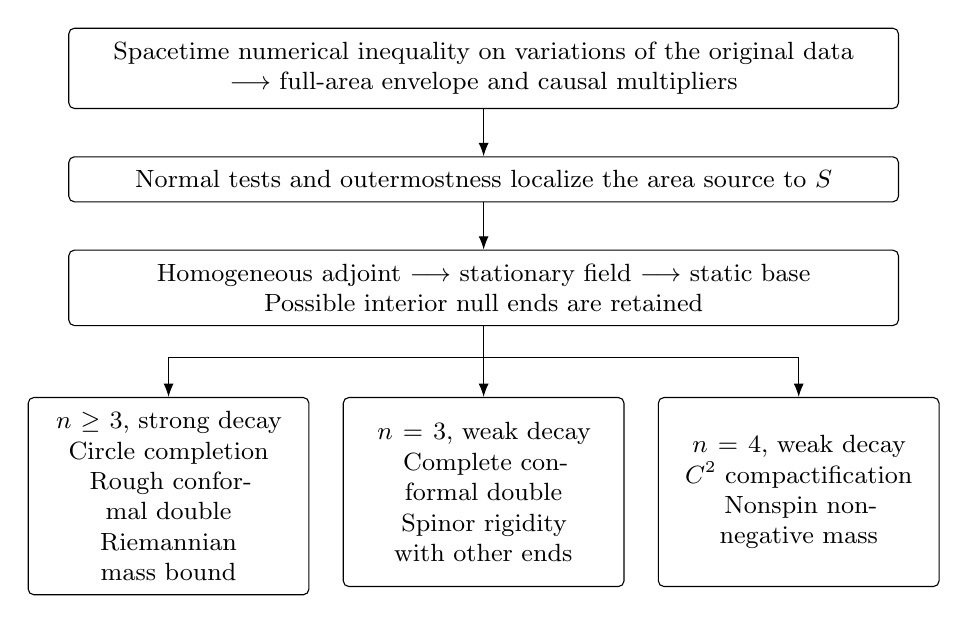
\begin{tikzpicture}[
 >=Latex,
 box/.style={draw,rounded corners=2pt,align=center,inner sep=5pt,
             font=\small},
 branch/.style={box,text width=.265\textwidth,minimum height=24mm},
 node distance=6mm]
\node[box,text width=.84\textwidth] (variation)
 {Spacetime numerical inequality on variations of the original data\\
  $\longrightarrow$ full-area envelope and causal multipliers};
\node[box,text width=.84\textwidth,below=of variation] (localization)
 {Normal tests and outermostness localize the area source to $S$};
\node[box,text width=.84\textwidth,below=of localization] (base)
 {Homogeneous adjoint $\longrightarrow$ stationary field $\longrightarrow$
  static base\\Possible interior null ends are retained};
\node[branch,below=9mm of base,xshift=-.33\textwidth] (strong)
 {$n\ge3$, strong decay\\Circle completion\\
  Rough conformal double\\Riemannian mass bound};
\node[branch,below=9mm of base] (three)
 {$n=3$, weak decay\\Complete conformal double\\
  Spinor rigidity with other ends};
\node[branch,below=9mm of base,xshift=.33\textwidth] (four)
 {$n=4$, weak decay\\$C^2$ compactification\\
  Nonspin nonnegative mass};
\draw[->] (variation)--(localization);
\draw[->] (localization)--(base);
\draw[->] (base.south)--(three.north);
\draw[->] (base.south) -- ++(0,-4mm) -| (strong.north);
\draw[->] (base.south) -- ++(0,-4mm) -| (four.north);
\end{tikzpicture}
\caption{The common variational and stationary steps precede three
complete classification arguments. Each branch proves the rigidity
needed for its conformal double and then recovers the original slice
through the horizon. Numerical mass bounds are used only in the
indicated roles.}
\label{fig:intro:proof}
\end{figure}

\subsection{Mathematical context and attribution}

Penrose's mass--area question arose from black-hole collapse and cosmic
censorship \cite{Penrose1973}. The area in an initial-data formulation
requires care. Ben-Dov constructed spherically symmetric data satisfying
the dominant energy condition for which the bound using the apparent
horizon's own area fails; he distinguished that area from the minimum
area needed to enclose it \cite[Section~1]{BenDov2004}. This distinction
explains the use of $a(g)$ in the numerical inequality and the separate
outer area-minimizing assumption in our equality classes.

For time-symmetric data, Huisken and Ilmanen's weak inverse mean
curvature flow proves the three-dimensional bound associated with a
connected horizon, while Bray's conformal flow gives the sharp bound
for the total area of a possibly disconnected horizon
\cite{HuiskenIlmanen2001,Bray2001}. Bray and Lee develop the conformal
flow in dimensions below eight \cite{BrayLee2009}. Minimizing hulls
and smooth-obstacle regularity are central to the inverse mean
curvature approach. Here perimeter compactness is combined with
Reshetnyak's continuity principle to differentiate the enclosing
infimum as the metric varies \cite{Reshetnyak1968,Spector2011}.

Beyond time symmetry, Bray and Khuri's generalized Jang construction
is an important equality precedent. In their spherically symmetric
setting they recover the original metric and second fundamental form
as a Schwarzschild spacelike embedding
\cite[Section~4]{BrayKhuri2010}. Their proposed nonspherical coupled
system is conditional on its existence and regularity
\cite[Section~5]{BrayKhuri2010}. The original-slice conclusion, rather
than vanishing of $K$, is thus already integral to the earlier
spacetime formulation. The argument here obtains that conclusion by
varying the original mass--area deficit after the numerical theorem
has been established.

Bartnik's variational program relates constrained gravitational
energy to stationary geometry. In his boundaryless asymptotically
flat three-dimensional phase space, critical points of the ADM energy
on a fixed constraint level set are characterized by the adjoint constraint
equations; future-timelike ADM vectors give the corresponding
invariant-mass formulation
\cite[Theorem~6.1 and Corollary~6.2]{Bartnik2005PhaseSpace}.
The Killing-initial-data framework and asymptotic Killing-field
estimates of Beig and Chru\'sciel explain how lapse--shift equations
encode a spacetime symmetry
\cite{BeigChrusciel1996,BeigChrusciel1997KID}.
For the dominant energy condition, Corvino and Huang introduce a
modified constraint operator that accounts for the metric dependence
of the momentum norm \cite[Section~2.2]{CorvinoHuang2020}.
Huang and Lee relate its adjoint, together with a null-vector identity,
to Killing developments with null-fluid stress
\cite[Section~6.1]{HuangLee2024Bartnik}.

Hirsch and Huang obtain a strongly stationary vacuum development of
the interior for local ADM-mass minimizers with compact boundary,
fixed Bartnik data, the dominant energy condition and $E>|P|$, under
their stated decay and regularity hypotheses
\cite[Theorem~7]{HirschHuang2025}. Fixing those boundary data fixes
$|S|$, but need not fix the least area of all enclosing cuts. Our
constrained minimum is therefore a different variational problem:
it retains $a(g)$ and the interior source generated by its minimizing
enclosures. Their strong maximum principle rules out an interior null
point for a causal Killing field $Y$ that is timelike near infinity
and satisfies $\operatorname{Ric}(Y,Y)\le0$
\cite[Theorem~4]{HirschHuang2025}. Here localization first produces the
homogeneous adjoint; the stationary construction retains its possible
null stress, and the twist argument treats the null set directly.

Static classification has its own ancestry. In three spatial
dimensions, Bunting and Masood-ul-Alam used positive mass to remove
the connected-horizon assumption in the asymptotically Euclidean
static vacuum problem \cite{BuntingMasoodUlAlam1987}.
Gibbons, Ida and Shiromizu developed the conformal construction in
higher dimensions \cite[Section~2]{GibbonsIdaShiromizu2002}.
Hwang's related rigidity theorem concerns complete spin Ricci-flat
manifolds with prescribed asymptotically flat behavior and an
appropriate circle action with fixed points
\cite{Hwang1998}; this is also a precedent for the circle-extension
setting used here. For the present data, we establish the completeness
of each double and the required horizon and compactified-point regularity.

The mass inputs are accordingly different in the three branches.
Bartnik and Chru\'sciel prove positive energy and parallel-spinor
rigidity with a noncompact interior
\cite[Theorem~11.2]{BartnikChrusciel2005}; Cecchini and Zeidler give a
smooth Riemannian spin formulation with arbitrary other ends and
Euclidean rigidity \cite[Theorem~B]{CecchiniZeidler2024}.
We supply the spinor argument at the rough regularity of the
three-dimensional double. In dimension four, Lesourd, Unger and Yau
supply smooth nonspin nonnegative mass for a distinguished
asymptotically Schwarzschild end, allowing arbitrary other ends
\cite[Theorem~1.2 and Definition~1.9, arXiv version~1]{LesourdUngerYau2021}.
We prove the required rigidity by deformation and volume comparison.
In the strong-decay branch, the Riemannian numerical companion
supplies the mass bound in every dimension from which the rough-double
rigidity is derived. None of these applications identifies a merely numerical
inequality with an equality theorem.

\subsection{Reading the proof}

Section~\ref{sec:setting} states the strong-decay equality theorem and
converse. Section~\ref{q:geometry:section} establishes the common
enclosure geometry and metric derivative.
Section~\ref{sec:variation} carries out the all-dimensional separation
and support localization; its smooth-dimensional shortcut is
identified after the contact argument. Section~\ref{sec:static}
contains the common stationary construction and the all-dimensional
classification, followed by the converse ADM calculation in
Section~\ref{q:converse:sec}.

For weak decay in dimension three, Sections~\ref{q3:intro:section}
and~\ref{q3:rigidity:setup} give the data and equality statements.
Variation and the static base lead to global classification and
horizon recovery in Section~\ref{q3:global:section}. A separate local
two-component spinor argument follows that main route. It examines a
family of complete conformal metrics and obtains a local obstruction
in the limit, without requiring completeness of the limiting metric.
It provides an alternative explanation of strictness for two spherical
components. The four-dimensional route begins in
Section~\ref{q4:sec:setup} and concludes with horizon recovery and the
weak-decay converse in Section~\ref{q4:rec:section}.

\section{Original data and the equality theorems}
\label{sec:setting}

Throughout, \(n\ge3\), \(k=n-1\), and
\(\omega=|S^{n-1}|\) is the area of the unit round sphere. The Laplacian
is \(\Delta=\divg\nabla\), and symmetrization includes the factor \(1/2\).
Mean curvature is the tangential divergence of the specified normal.

\begin{definition}[One-ended initial-data exterior]
\label{def:data}
A one-ended initial-data exterior is a smooth connected orientable
\(n\)-manifold \(\Omega\) with nonempty compact smooth boundary \(S\),
a smooth Riemannian metric \(g\), and a smooth symmetric covariant
two-tensor \(K\), both smooth up to \(S\), satisfying the following
conditions.

The metric space \((\Omega,g)\), with \(S\) included, is complete.
There is a compact subset \(C\subset\Omega\) such that
\(\Omega\setminus C\) is a single coordinate end diffeomorphic to
\(\{x\in\R^n:|x|>R_0\}\). In these coordinates, for some
\[
 \frac{n-2}{2}<q<n-2,
\]
we have
\begin{equation}
 g_{ij}-\delta_{ij}=O_6(r^{-q}),\qquad
 K_{ij}=O_5(r^{-1-q}),\qquad r=|x|.
 \label{eq:setting:decay}
\end{equation}
Here \(O_j(r^{-a})\) includes the estimate
\(|\partial^\alpha T|\le C_\alpha r^{-a-|\alpha|}\) for every
\(|\alpha|\le j\). These are asymptotic bounds on otherwise smooth data.

Put
\begin{equation}
 \tau=\tr_gK,\qquad
 2\mu=R_g+\tau^2-|K|_g^2,\qquad
 J_i=\nabla^j(K_{ij}-\tau g_{ij}).
 \label{eq:setting:constraints}
\end{equation}
We assume the dominant energy condition and integrability:
\begin{equation}
 \mu\ge |J|_g,\qquad
 \mu,\ |J|_g\in L^1(\Omega,dV_g).
 \label{eq:setting:dec}
\end{equation}
The ADM limits
\begin{align}
 E&=\frac{1}{2k\omega}
 \lim_{R\to\infty}\int_{S_R}
   (\partial_jg_{ij}-\partial_ig_{jj})\,n_\delta^i\,dA_\delta,
 \label{eq:setting:energy}\\
 P_i&=\frac{1}{k\omega}
 \lim_{R\to\infty}\int_{S_R}
  (K_{ij}-\tau g_{ij})\,n_\delta^j\,dA_\delta
 \label{eq:setting:momentum}
\end{align}
exist and are finite. We impose the future-timelike condition
\begin{equation}
 E>|P|_\delta,\qquad m=(E^2-|P|_\delta^2)^{1/2}.
 \label{eq:setting:timelike}
\end{equation}

On every component of \(S\), the unit normal \(\nu\) points into
\(\Omega\). We require
\begin{equation}
 \theta_+(S)=H_S+\tr_SK\le0,\qquad
 H_S=\divg_S\nu,\qquad
 \tr_SK=(g^{ij}-\nu^i\nu^j)K_{ij}.
 \label{eq:setting:trapping}
\end{equation}
There is no assumption on the other null expansion.
\end{definition}

The compact-complement condition in Definition~\ref{def:data} is part of
our use of \emph{one-ended}. It excludes additional non-asymptotically-flat
ends. Merely specifying one asymptotically flat end among other
unrestricted ends would define a larger class, for which the compact
filling and global arguments below would need additional hypotheses.
The cosmological constant is zero. No spin, maximality, time-symmetry,
vacuum, stationary-development, or interior-topology assumption is made.

\begin{definition}[Full enclosing cuts]
\label{def:fullcuts}
A full enclosing cut is \(\Gamma=\partial D\), the entire intrinsic
manifold boundary of a connected smooth codimension-zero
submanifold-with-boundary \(D\) of \(\Omega\), such that \(D\) is closed
in \(\Omega\), its manifold interior lies in \(\operatorname{int}\Omega\),
and it contains the whole sufficiently distant coordinate end.
We require \(\Gamma\) to be compact, smooth, embedded, and two-sided.

All components of \(\partial D\) are counted, including any portion
coincident with \(S\). In particular, \(D=\Omega\) is admissible and
has full boundary \(S\). Define
\begin{equation}
 A_{\min}(S)=\inf_{\Gamma}\Area_g(\Gamma),
 \label{eq:setting:minarea}
\end{equation}
and assume \(A_{\min}(S)>0\).
\end{definition}

A cut need not be connected, minimal, or trapped. The areas in
\eqref{eq:setting:minarea} are always computed in the original metric
\(g\). We neither assume that the infimum is attained nor assign a
classical expansion to a singular minimizing boundary.

\begin{theorem}[Numerical input]\label{thm:numerical-input}
The numerical spacetime Penrose theorem \cite[Theorem~1.3]{CompanionNumerical} states that every initial-data exterior in Definition~\ref{def:data}, with
the positive full-cut infimum in Definition~\ref{def:fullcuts}, satisfies
\begin{equation}
 \boxed{\quad
 m\ge\frac12
 \left(\frac{A_{\min}(S)}{\omega}\right)^{\frac{n-2}{n-1}} .
 \quad}
 \label{eq:setting:main}
\end{equation}
This input is used for nearby weakly trapped data as well as for the
original pair. It imposes none of the additional equality hypotheses
introduced below.
\end{theorem}

The normalization is geometric: the Schwarzschild--Tangherlini metric
of mass \(M>0\) is
\begin{equation}
 \begin{gathered}
 \mathbf G_M=-F(r)\,dt^2+F(r)^{-1}\,dr^2+r^2\sigma_{n-1},\\
 F(r)=1-\frac{2M}{r^{n-2}},\qquad
 r>r_M:=(2M)^{1/(n-2)}.
 \end{gathered}
 \label{eq:setting:tangherlini}
\end{equation}
Here \(\sigma_{n-1}\) is the unit round metric. We use its regular
extension across the future horizon and at the bifurcation sphere.
For a spacelike hypersurface our sign convention is
\begin{equation}
 K(U,V)=\mathbf G_M(\nabla^{\mathbf G_M}_U n_{\mathrm{future}},V).
 \label{eq:setting:Ksign}
\end{equation}

\begin{definition}[Rigidity class]
\label{def:setting:rigidity}
An exterior in Definition~\ref{def:data} belongs to the rigidity class
if \(S\) is connected, \(\theta_+(S)=0\), every full cut has area at
least \(A=\Area_g(S)>0\), and no compact smooth embedded two-sided
enclosing hypersurface entirely in \(\operatorname{int}\Omega\),
possibly disconnected, has \(\theta_+\le0\) everywhere with normal
toward the end.
\end{definition}

Thus \(A_{\min}(S)=A\) in this class. Outermostness is imposed only for
smooth entirely interior enclosing hypersurfaces; its use on limiting
minimizers will be justified by the singular-sheet argument.

\begin{theorem}[Original-data rigidity]
\label{thm:rigidity}
Suppose an exterior in Definition~\ref{def:setting:rigidity} attains
equality in \eqref{eq:setting:main}. There is a global smooth spacelike
embedding of the entire \(\Omega\), including \(S\), into the regular
extension of one exterior of \(\mathbf G_m\), inducing exactly the
original \(g\) and \(K\) with convention \eqref{eq:setting:Ksign}.

The image lies in the domain \(r>r_m\) together with its corresponding
future horizon and bifurcation sphere. The boundary maps to a full
smooth section of that future horizon or to its bifurcation sphere.
The embedding and future unit normal extend smoothly to \(S\) in
horizon-regular coordinates, and the chosen end approaches spatial
infinity. There is no conclusion about a region behind \(S\).
\end{theorem}

A full horizon section meets every null generator once; its induced
metric has the same area as the round horizon sphere. In statements
about an asymptotic slice, approaching spatial infinity means that
the ambient static radius tends to infinity along every sequence
escaping the given coordinate end.

\begin{theorem}[Converse and sharpness]
\label{thm:converse}
Let \(M>0\). Every smooth spacelike exterior hypersurface in the regular
extension of \(\mathbf G_M\), with its interior in \(r>r_M\), whose
induced data satisfy
Definitions~\ref{def:data}, \ref{def:fullcuts}, and
\ref{def:setting:rigidity}, whose boundary is a full smooth section
of the corresponding future horizon or its bifurcation sphere,
and whose end approaches spatial infinity, has
\begin{equation}
 (E^2-|P|_\delta^2)^{1/2}=M,\qquad
 A=\omega(2M)^{\frac{n-1}{n-2}}.
 \label{eq:setting:converse}
\end{equation}
It therefore attains equality in \eqref{eq:setting:main}.
In every dimension there are admissible static examples and
admissible examples with \(K\not\equiv0\).
\end{theorem}

Theorems~\ref{thm:rigidity} and \ref{thm:converse} permit
non-time-symmetric and asymptotically boosted slices. The invariant
mass assertion in the converse refers to the original slice's ADM
integrals \eqref{eq:setting:energy}--\eqref{eq:setting:momentum};
it is not inferred only from an auxiliary Riemannian metric.


\subsection{The strict direction used in the variation}

The numerical inequality applies on a constraint set with boundary:
the dominant energy condition and the expansion condition may both be
saturated. The following analytic input supplies a direction into its
interior. Its proof is independent of the numerical inequality.

\begin{lemma}[Strict conformal direction]\label{lem:strict-input}
For the smooth exterior and decay in Definition~\ref{def:data}, choose
$0<\beta<\min(1,q)$ and a smooth positive extension $\varrho$ of the
coordinate radius. Let $B\geq|K|$ be smooth and nonnegative, with
$B=O_5(r^{-1-q})$. There is a unique smooth positive solution tending
to zero at infinity of
\[
 -\Delta_g\phi=B\sqrt{|d\phi|_g^2+\varrho^{-2k}}
                    +\varrho^{-n-\beta},\qquad
 \partial_\nu\phi=-1\quad\hbox{on }S.
\]
It satisfies $\phi=O_6(r^{2-n})$, and
$(-\Delta_g\phi)/r^{-n-\beta}\to1$. Its flux is finite and equals
\[
 f_\phi:=\lim_{R\to\infty}\int_{S_R}\partial_{\nu_g}\phi\,dA_g
 =-\Area(S)-\int_\Omega
 \left[B\sqrt{|d\phi|^2+\varrho^{-2k}}+\varrho^{-n-\beta}\right]dV_g<0.
\]
For sufficiently small $\delta>0$, the pair
$(e^{2\delta\phi}g,e^{\delta\phi}K)$ satisfies a strict global
weighted dominant energy inequality and has strictly negative future
expansion. Its energy is $E-\delta f_\phi/\omega$, its momentum is
$P$, and its metric is at least $g$ and converges uniformly relative
to $g$ as $\delta\downarrow0$.
\end{lemma}

This is the strict-direction lemma in the numerical companion
\cite[Lemma~3.5]{CompanionNumerical}; its
complete exterior proof accompanies that numerical theorem. Below we
also compute the precise active-ray derivative, since its positivity
is the part needed for separation.

\subsection{How the dimension-dependent conclusions fit together}

Theorem~\ref{thm:rigidity} concerns a one-ended exterior with strong
differentiated decay and requires no ambient extension behind its
boundary. There are further conclusions for weaker decay in spatial
dimensions three and four. Their precise hypotheses and statements
appear in Theorems~\ref{q3:intro:rigidity},
\ref{q3:intro:connected-rigidity}, and~\ref{q4:thm:rigidity}.

The three-dimensional statements assume a complete boundaryless
ambient initial-data manifold with finitely many asymptotically flat
ends. The finite-component version forbids weakly trapped enclosing
cuts even when they partly coincide with the given horizon; it forces
one spherical component. With a connected boundary, the weaker
wholly-interior outermostness condition suffices. These weak-decay
statements are forward rigidity results. The four-dimensional
statement is an exterior theorem, with a connected marginal
outer-area-minimizing horizon and wholly-interior outermostness; it
also includes its horizon-regular converse.

The distinction matters for the proof. The all-dimensional argument
excludes possible interior null ends by a circle extension before
forming a compact-core double. The low-dimensional classification
arguments permit such ends while applying their positive-mass inputs.
We will therefore match regularity and completion separately in each
branch, after localizing the original-data variational equations.

\section{Minimizing enclosures and their area envelope}
\label{q:geometry:section}

The area in the numerical inequality is an infimum over complete
enclosing frontiers. A metric perturbation can change which frontier
attains that infimum. We first describe the whole family of minimizers
and then differentiate its least area. This argument concerns only the
metric and the enclosing sets; no constraint equation or equality
hypothesis enters it.

Let $(X,g)$ be a connected orientable smooth $n$-manifold, $n\ge3$,
complete with its nonempty compact smooth boundary $B$ included.
The boundary may be disconnected. Assume that outside a compact set
$X$ is one Euclidean coordinate end and
\begin{equation}\label{q:geometry:AF}
 g-\delta=O_2(r^{-q}),\qquad q>0.
\end{equation}
A full cut is the entire compact smooth embedded two-sided intrinsic
boundary of a connected closed outer domain in $X$, whose interior
lies in $\operatorname{int}X$ and which contains the distant end.
Every boundary component and every portion coincident with $B$ is
counted. Write $a(g)$ for the infimum of their full areas.

Attach a compact smooth filling $O$ behind $B$ and extend the metric
smoothly to the resulting boundaryless manifold $\widehat X$. Such a
filling exists here: reverse a compact truncation of $X$ and cap its
spherical end boundary with a ball. The remaining boundary is the
oppositely oriented $B$. The filling and collar extension serve only
to measure perimeter on $B$; the metric farther inside $O$ has no role.
Let $\mathcal A$ be the bounded finite-perimeter sets $E\subset\widehat X$
containing $O$ almost everywhere, identified modulo null sets. Put
\begin{equation}\label{q:geometry:full-perimeter}
 P_g(E)=|D\mathbf1_E|_g(\widehat X),\qquad
 T_E=\operatorname{supp}|D\mathbf1_E|_g,
 \qquad \mathcal T(g)=\operatorname*{argmin}_{E\in\mathcal A}P_g(E).
\end{equation}
Thus the perimeter is measured in the filled manifold, including
contact with $B$. A smooth full cut bounds a filled set of precisely
the same perimeter; in particular $P_g(O)=\operatorname{Area}_g(B)$.
We use the basic BV compactness, Gauss--Green and submodularity facts
in \cite{AmbrosioFuscoPallara2000,Maggi2012}.

\subsection{Existence, contact regularity, and strict barriers}

\begin{proposition}[The full minimizing enclosure]
\label{q:geometry:enclosure}
The minimum in Equation~\eqref{q:geometry:full-perimeter} exists,
equals $a(g)>0$, and is independent of the filling. All its minimizing
sets are contained in one compact region. Their multiplicity-one
frontiers are smooth minimal hypersurfaces away from $B$ and a
singular set of Hausdorff dimension at most $n-8$; the singular set is
empty when $n\le7$. Every contact point with $B$ is regular, with a
$C^{1,\alpha}\cap W^{2,p}$ graph for every finite $p$ and
$0<\alpha<1$. For $n=3,4$ the whole frontier is $C^{1,1}$, including
contact, and its graph functions are $W^{2,\infty}$.

In dimensions $3$ and $4$, each frontier bounds a connected exterior
and is the $C^1$ and area limit of smooth full cuts contained in
$\operatorname{int}X$. If $H_B<0$ for the normal into $X$, every
minimizer contains one fixed exterior collar of $B$. In dimensions
$3$ and $4$ its frontier is then a smooth minimal full cut; its closed
exterior is connected, one-ended, complete with its boundary included,
and outer area-minimizing with all boundary components counted.
In every dimension, whenever a minimizing frontier is smooth, its
closed exterior has these same connectedness, completeness, one-end
and outer area-minimization properties.
\end{proposition}

\begin{proof}
\emph{Confinement and existence.}
For sufficiently large $R_0$ the end spheres have
\[
 H_{\{r=R\}}=\operatorname{div}_g
       (\nabla r/|\nabla r|_g)
       =\frac{n-1}{R}+O(R^{-1-q})>0.
\]
Set $Y=\nabla r/|\nabla r|_g$. For each competitor $E$, and almost
every $R>R_0$, the BV trace formula and Gauss--Green on
$E\cap\{r>R\}$ give
\begin{equation}\label{q:geometry:clipping}
 P_g(E\setminus\{r>R\})-P_g(E)
 \le-\int_{E\cap\{r>R\}}\operatorname{div}_gY\,dV_g\le0.
\end{equation}
Indeed the new slice area is the flux through the inner end of this
region; the original exterior-boundary flux is at most its perimeter.
At a good slicing radius the two traces agree, so these are exactly
the terms in the perimeter difference. The inequality is strict if
the removed set has positive volume.

Fix $R_1>R_0$. For each competitor choose a good radius in
$(R_0,R_1)$ and clip there. This confines a minimizing sequence to
the same compact region. BV compactness and lower semicontinuity
produce a global minimizer; containment of $O$ and emptiness in the
fixed tail are closed constraints. Applying the strict inequality to
any minimizer, at a good radius below a fixed $R_2$ with
$R_0<R_2<R_1$, puts every minimizer inside the smaller truncation.
There is no need for a radius that is simultaneously a good slice
for every competitor.

\emph{Recovering the full smooth-cut infimum.}
A full cut supplies a member of $\mathcal A$, so
$\min P_g\le a(g)$. In the other direction choose a smooth collar
field pointing strictly out of $O$ on $B$ and let $\Phi_\varepsilon$
be its flow. For small positive $\varepsilon$, the set
$\Phi_\varepsilon(E)$ contains a neighborhood of $O$, and its
perimeter tends to $P_g(E)$. Approximate its indicator in finitely
many charts by convolution and a partition of unity, keeping it
identically one on a smaller neighborhood of $O$ and zero outside a
fixed compact region. The BV approximation and coarea formula give
smooth level sets containing that neighborhood, with perimeters
tending to $P_g(\Phi_\varepsilon(E))$.
Fill every bounded complementary component of such a level set and
retain the complementary component containing the end. Its closure
in $X$ is a connected smooth outer domain; filling deletes boundary
components and creates none. Its full-cut area is no larger than the
approximating perimeter. Letting the approximation error, then
$\varepsilon$, tend to zero proves $a(g)\le P_g(E)$. This argument
also works when $E$ has singular frontier.

\emph{Local regularity.}
Choose a smooth field $Z$ supported near $B$, with $|Z|_g\le1$ and
$Z=\nu_O$ on $B$. For any local replacement $F$ of a minimizer $E$,
submodularity, constrained minimality, and Gauss--Green imply
\begin{align*}
 P_g(E)&\le P_g(F\cup O)
       \le P_g(F)+P_g(O)-P_g(F\cap O),\\
 P_g(O)-P_g(F\cap O)&\le
       \int_{O\setminus F}\operatorname{div}_gZ\,dV_g
       \le C\operatorname{Vol}_g(E\triangle F).
\end{align*}
The unchanged terms outside the replacement region cancel. Thus, if
$E\triangle F\Subset U$,
\begin{equation}\label{q:geometry:almost-minimality}
 P_g(E;U)\le P_g(F;U)+C\operatorname{Vol}_g(E\triangle F).
\end{equation}
Ball insertion and deletion, followed by the relative isoperimetric
inequality, give an upper perimeter bound $Cr^{n-1}$ and positive
lower density bounds for both phases at every frontier point
\cite{Maggi2012}. The
volume error in Equation~\eqref{q:geometry:almost-minimality} scales
as $r^n$. The local almost-minimizing-boundary theorem gives
$C^{1,\alpha}$ regularity at reduced-boundary points and minimizing
boundary cones as tangent sets. Dimension reduction gives singular
dimension at most $(n-1)-7=n-8$; see
\cite[Theorem~2.27]{BiZhu2026} and the codimension-one theory in
\cite[Chapter~7]{Simon2018}. Off the obstacle the minimizing property
has zero error, so the regular frontier is smooth and minimal.

At a contact point a tangent filled set contains the tangent
half-space of $O$. Its stationary boundary cone lies on one side of
the bounding plane. Such a cone is planar: the nonnegative height
function on its spherical link satisfies weakly
$\Delta_{\rm link}z=-(n-2)z$. Testing with the constant function
makes its height integral zero, hence its support lies in the plane.
The weak stationary identity is on the whole link and does not
discard its singular set. The two density bounds and the
multiplicity-one boundary property select a half-space rather than
the full or empty set. Density regularity therefore makes the contact
point a graph point.

Equation~\eqref{q:geometry:almost-minimality}, applied to flows with
both signs, bounds the graph's weak mean curvature. Its scalar
minimal-surface operator has smooth coefficients and is uniformly
elliptic on the bounded gradient range. Difference quotients yield
$W^{2,2}$ locally. In nondivergence form the leading coefficients
are $C^{0,\alpha}$ and the right side is bounded; localized linear
$W^{2,p}$ estimates then give every finite $p$. The Sobolev embedding
allows every $\alpha<1$. In dimensions $3$ and $4$ we also use the
stronger smooth-obstacle theorem: for a $C^2$ obstacle, zero bulk
term, and ambient dimension below eight, its entire minimizing
frontier is $C^{1,1}$
\cite[Regularity Theorem~1.3(iii), pp.~368--369]{HuiskenIlmanen2001}.
This gives the stated $W^{2,\infty}$ regularity.

The frontier is nonempty. Otherwise its BV indicator is constant
on the connected filled manifold, contrary to containment of the
open obstacle and absence from an end tail. Its perimeter is positive;
this follows from the relative isoperimetric inequality, or from a
regular frontier chart.

\emph{Connected exterior and smooth approximation in low dimensions.}
Take the closure of the measure-theoretic interior as representative.
When $n=3,4$ its frontier is compact embedded $C^{1,1}$, with filled
and exterior sets on its two local sides. Any complementary component
other than the end component is relatively compact. Its boundary is
a nonempty union of frontier components. Filling it removes positive
full perimeter, contradicting minimality. The exterior is connected. The same argument applies in every
dimension whenever the frontier is smooth. It only uses the local
two-sided hypersurface charts and compactness.

Choose a smooth field $V$ uniformly transverse to the continuous
outward normal of the compact frontier $T$. Its flow gives a $C^1$
collar $\Psi:T\times(-\delta,\delta)\to\widehat X$ with filled side
$t\le0$. For small $\varepsilon>0$, the flowed set is
$E\cup\Psi(T\times(0,\varepsilon])$; every crossing of the frontier
is outward. It contains $O$ in its interior, and the displaced
frontier lies at positive distance from $B$. Smooth a $C^1$ defining
function in a smaller collar, retaining its positive derivative
along $V$. The resulting smooth zero set is a small graph on the
collar fibers. Extend the graph displacement to an isotopy supported
in that collar; it fixes $O$ and the distant end. Enclosure and
connectedness of the exterior are therefore preserved. The resulting
full cuts converge in $C^1$ and area to $T$.

\emph{Detachment from a strict inner barrier.}
If $H_B<0$ for the normal into $X$, a fixed distance collar
$0\le t\le\varepsilon$ has $Y=\partial_t$ and
$\operatorname{div}_gY\le-\beta<0$. For a good level $s$, put
$O_s=O\cup\{0<t<s\}$ and $W_s=O_s\setminus E$.
Gauss--Green on $W_s$, including the flux on $t=0$, gives
\begin{equation}\label{q:geometry:detachment}
 P_g(E\cup O_s)-P_g(E)
 \le\int_{W_s}\operatorname{div}_gY\,dV_g
 \le-\beta\operatorname{Vol}_g(W_s).
\end{equation}
Minimality makes $W_s$ null. Choosing, for each minimizer, a good
$s\in(\varepsilon/2,\varepsilon)$ proves that the same smaller
collar lies in its filled interior. Thus all contact is removed.

For $n=3,4$ the detached frontier is now smooth and minimal. More
generally, in any dimension where the frontier under consideration
is smooth, its connected closed exterior $D$ contains just the original end. It is complete
in its intrinsic length metric: an intrinsic Cauchy sequence is
Cauchy in $X$, has a limit in the closed set $D$, and smooth interior
or boundary half-ball charts give intrinsic convergence to that
limit. Finally, every full enclosing cut of $D$ gives a filled
competitor containing $E$ and hence $O$. Its full area is at least
$P_g(E)$. This proves outer area-minimization with every component
and all coincidence counted.
\end{proof}

\subsection{Continuity of planes before differentiation}

For $E\in\mathcal T(g)$ define the position-and-plane measure $V_E$
on the bundle of unoriented $(n-1)$-planes by
\begin{equation}\label{q:geometry:plane-measure}
 \int\Phi\,dV_E=
 \int_{\partial^*E}\Phi(x,T_x\partial^*E)\,dA_g.
\end{equation}
Singular points have zero perimeter measure. Give $\mathcal T(g)$
the topology of $L^1$ convergence of indicators and weak convergence
of these measures. The next result explains why its second requirement
follows from the first, and why it is needed for the metric derivative.

\begin{proposition}[Compactness and the derivative of least area]
\label{q:geometry:envelope}
The space $\mathcal T(g)$ is compact and metrizable. For every smooth
symmetric two-tensor $h$ the function
\[
 E\longmapsto a'_E(h):=
 \frac12\int_{\partial^*E}\operatorname{tr}_{T\partial^*E}h\,dA_g
\]
is continuous on it.
Let $g_t$, $|t|<t_0$, be a smooth path of smooth metrics with $g_0=g$,
extended smoothly through the fixed boundary. Assume uniform
comparison with $g$, and bounded first and second parameter derivatives
relative to $g$. One sufficient end hypothesis is
\begin{equation}\label{q:geometry:uniform-AF}
 g_t-\delta=O_2(r^{-q_*})\quad\hbox{uniformly for }|t|<t_0,
 \qquad q_*>0.
\end{equation}
More generally, it suffices that the coordinate spheres have positive
outward mean curvature beyond one common radius. The result also
holds if the end metrics are uniformly comparable to the Euclidean
metric with uniform scaled $C^1$ bounds; they need not have a common
mean-convex tail in this last alternative. Put $h=\partial_tg_t|_0$. Then
\begin{equation}\label{q:geometry:envelope-derivative}
 \left.\frac{d}{dt}\right|_{0+}a(g_t)
       =\min_{E\in\mathcal T(g)}a'_E(h).
\end{equation}
For any $t_j\to0$ and any $E_j\in\mathcal T(g_{t_j})$, a subsequence
converges in $L^1$ to $E\in\mathcal T(g)$, with convergence of
perimeters and of the plane measures computed in the fixed metric $g$.
\end{proposition}

\begin{proof}
The uniform asymptotic hypothesis gives one mean-convex tail, so
Equation~\eqref{q:geometry:clipping} confines all minimizers uniformly.
The same proof applies under the common-sphere hypothesis. For the
last alternative, existence can be proved without an outer barrier.
Minimize inside successively larger closed coordinate truncations.
Each constrained minimum exists by the direct method and is at most
$P_{g_t}(O)$. Local BV compactness yields a limiting set containing
$O$, of finite total perimeter. The minimizing values decrease to the
infimum over bounded competitors. The limit is locally minimizing
away from $O$, and constrained-minimizing at $O$: to compare it with
a compact replacement, glue that replacement into the truncated
minimizers across a thin annulus. Coarea chooses a slicing boundary
on which the $L^1$ trace discrepancy tends to zero, so the added
perimeter tends to zero. The minimizing inequality then passes to
the limit. This is the local minimizing-boundary compactness argument
in the BV framework of \cite{AmbrosioFuscoPallara2000,Maggi2012}.

The limit has finite volume, so its exterior phase is the empty one
once its frontier is confined. To see the finite-volume assertion
before using confinement, apply the Euclidean isoperimetric inequality
to the filled part on the coordinate end with a fixed inner slicing
sphere, capping that slice inside the coordinate ball. Its Euclidean
perimeter is bounded by the original perimeter times the uniform
metric-comparison constant, plus the fixed sphere area. The resulting
volume bound is uniform in the outer truncation; local convergence
passes it to the limit.

Testing on $O$ gives a uniform perimeter bound. If a minimizing frontier passes through an
end point of radius $r$, a coordinate ball of radius $cr$ about that
point misses the obstacle. The rescaled metrics are uniformly elliptic
with uniformly bounded first derivatives, and the frontier is locally
perimeter-minimizing in that ball. The interior perimeter density
estimate gives area at least $c_1r^{n-1}$, with $c_1$ uniform. This
contradicts the fixed upper bound for large $r$. Thus the limiting
frontier lies in a fixed compact region. The connected end tail is
therefore almost everywhere full or empty; finite volume makes it
empty. The limiting set is an admissible bounded competitor. Lower
semicontinuity bounds its perimeter by the infimum approached by the
truncated minima, so it is a global minimizer. The same density argument
confines every global minimizer, uniformly in $t$. Thus their bounded
filled sides again lie in one compact set.

BV compactness now applies on that compact region. For fixed-metric
minimizers $E_j\to E$ in $L^1$, lower semicontinuity gives
\[
 a(g)\le P_g(E)\le\liminf_jP_g(E_j)=a(g).
\]
Thus the limit is a minimizer and the perimeters converge. Set
$\sigma_j=|D\mathbf1_{E_j}|_g$ and $\sigma=|D\mathbf1_E|_g$.
Weighted lower semicontinuity makes every weak limit of $\sigma_j$
dominate $\sigma$. Their total masses agree, so
$\sigma_j\rightharpoonup\sigma$. The normal vector measures
$\nu_j\sigma_j$ converge weakly to $\nu\sigma$ by Gauss--Green.

To pass from normals to tangent planes, cover the compact support by
finitely many charts with nonnegative smooth partition weights
$\rho_\alpha$. Choose a smooth matrix $A_\alpha(x)$ in each chart
such that $|A_\alpha(x)v|_\delta=|v|_g$. The Euclidean vector measures
\[
 \lambda_{\alpha,j}=\rho_\alpha A_\alpha\nu_j\sigma_j
 \quad\hbox{have}\quad
 |\lambda_{\alpha,j}|_\delta=\rho_\alpha\sigma_j.
\]
They converge weakly and their total variations have convergent
masses. The localized Reshetnyak continuity theorem
\cite{Reshetnyak1968}, in the polar-direction formulation of
\cite[Theorem~1.3]{Spector2011}, therefore applies to
\[
 (x,z)\longmapsto
 \Phi\bigl(x,(A_\alpha(x)^{-1}z)^{\perp_g}\bigr),
 \qquad |z|_\delta=1.
\]
Insert a continuous compact cutoff equal to one on the localized
support, so the integrand is bounded on the chart, and sum over the
partition. This proves weak convergence of $V_{E_j}$, including
contact mass: a chart crossing $B$ is an interior chart of
$\widehat X$. It is convergence of plane integrals, not yet pointwise
convergence of tangent planes. Compact supports and bounded masses
make the indicated measure topology metrizable. The subsequence
argument proves compactness, and the choice
$\Phi(x,\Pi)=\frac12\operatorname{tr}_\Pi h$ proves continuity.

For varying metrics, uniform convergence on the confining region
provides $\varepsilon_t\to0$ such that
\[
 (1-\varepsilon_t)P_g(F)\le P_{g_t}(F)
              \le(1+\varepsilon_t)P_g(F)
\]
for every confined competitor. Testing a fixed $g$-minimizer and
using $P_g(E_t)\ge a(g)$ shows
$a(g_t)\to a(g)$ and $P_g(E_t)\to a(g)$. Hence every BV limit is a
$g$-minimizer and the preceding localized argument gives its plane
measure convergence.

On the compact Grassmann bundle the area density has the uniform
Taylor expansion
\begin{equation}\label{q:geometry:area-taylor}
 P_{g_t}(F)=P_g(F)+t\,a'_F(h)+O(t^2)P_g(F).
\end{equation}
Testing every fixed $E\in\mathcal T(g)$ gives
$\limsup_{t\downarrow0}(a(g_t)-a(g))/t\le\min_Ea'_E(h)$.
For the other bound choose $E_t\in\mathcal T(g_t)$. Its $g$-perimeter
is uniformly bounded and at least $a(g)$, so
\[
 \frac{a(g_t)-a(g)}t\ge a'_{E_t}(h)-O(t).
\]
Every sequence tending to zero has a subsequence whose plane measures
converge to those of a $g$-minimizer. The right side then tends to a
value at least $\min_Ea'_E(h)$. This proves both the derivative and
its formula, with no uniqueness or smooth choice of a minimizing cut.
\end{proof}

\subsection{Tied sheets and uniform graphical separation}

The averaged area source later requires one plane at a point shared
by different minimizing frontiers. It also requires quantitative
control when a nearby frontier approaches a given regular sheet.
These are local consequences of minimizing geometry, distinct from
the integral continuity just proved.

\begin{proposition}[No crossing and uniform regular sheets]
\label{q:geometry:sheets}
If a minimizing frontier meets the free regular part of another,
the two frontiers agree locally at that point. In particular the
plane field on the union of their free regular parts is well-defined
and continuous in its relative topology. Around every such point
there are nested graph cylinders, disjoint from $B$, in which every
minimizing frontier meeting the smaller cylinder is a single smooth
graph over the same base. The graph bounds are uniform on smaller
base domains. Two such graphs either agree or are disjoint and can
be ordered. For $V'\Subset V$ and fixed $y_0\in V$, their ordered
heights obey
\begin{equation}\label{q:geometry:graph-separation}
 \|h_1-h_2\|_{C^j(V')}\le C_j|h_1(y_0)-h_2(y_0)|,
 \qquad j=0,1,2,\ldots,
\end{equation}
with constants uniform in the two minimizers.
\end{proposition}

\begin{proof}
For minimizing sets $E,F$, submodularity gives
\[
 P_g(E\cup F)+P_g(E\cap F)\le P_g(E)+P_g(F)=2a(g).
\]
Each term on the left is at least $a(g)$, so the union and
intersection are themselves minimizers and the submodularity deficit
is zero as a measure. Let $x\in T_F$ lie on a free regular sheet of
$T_E$. Blow up both sets at $x$ along a common sequence, writing
$H$ for the tangent half-space of $E$ and $C$ for a tangent set of
$F$. Their unions and intersections converge in $L^1$ to $C\cup H$
and $C\cap H$. Minimizing-boundary compactness makes these minimizing
cones, with empty and full sets allowed. The half-space argument in
Proposition~\ref{q:geometry:enclosure} gives
\[
 C\cup H\in\{H,\mathbb R^n\},\qquad
 C\cap H\in\{\varnothing,H\}.
\]
Thus $C$ is one of $H,H^c,\varnothing,\mathbb R^n$; the density
bounds for $F$ rule out the latter two.

If $C=H$, both union and intersection have density-one planar tangent
and are regular near $x$. Their minimal graphs are ordered against
the reference sheet and touch it at $x$. The strong comparison
principle makes them agree with it locally, hence so does $T_F$.
If $C=H^c$, the union has full tangent and the intersection empty
tangent. The uniform two-phase density bounds at frontier points
put $x$ outside the supports of both boundaries. In a neighborhood
the union is full and the intersection empty, so $F$ is the complement
of $E$ there. Their common open sheet contributes twice its positive
area to $P_g(E)+P_g(F)$ and zero to the union and intersection.
That contradicts the zero submodularity deficit. This excludes the
opposite coorientation and proves local agreement.

We next justify the uniform graphical assertion, including the
entire support. Suppose $x_j\in T_{E_j}$ tends to a free regular
point $x$ of a fixed minimizing frontier. Compactness from
Proposition~\ref{q:geometry:envelope} gives a minimizing limit
$E_\infty$. Uniform density bounds put $x\in T_{E_\infty}$, and
the preceding argument identifies its sheet near $x$ with the fixed
regular sheet. In a ball about $x$ missing $B$, all these boundaries
are locally area-minimizing. Their integral varifolds are stationary
in the smooth ambient metric, with multiplicity one and no boundary.
The limit is smooth with density one.

Choose a sufficiently small continuity radius for its area measure.
The limiting mass ratio is close to one and its height and tilt
excesses relative to $T_xT_{E_\infty}$ are small. Plane-measure
convergence transfers these properties to $E_j$. Moving centers to
$x_j$ changes the required radii by a quantity tending to zero.
To apply the small-excess theorem in a Riemannian chart, use its
smooth-ambient form, or smoothly isometrically embed a neighborhood:
stationarity in the ambient manifold gives Euclidean generalized
mean curvature bounded by the ambient second fundamental form.
After rescaling by the small radius, the required $L^p$ curvature
norm is small for any fixed $p>n-1$.

Allard's graphical theorem therefore represents the entire support
in a smaller ball by a single $C^{1,\alpha}$ graph with uniform bounds
\cite{Allard1972,Maggi2012}; the exact small-mass and $L^p$ mean-curvature
formulation is \cite[Chapter~5, Section~5, Theorem~5.2]{Simon2014}.
It leaves no second small sheet or spike outside a selected graphical
component. Uniform graph compactness and the identified varifold
limit give $C^1$ convergence; interior estimates for the smooth
minimal-graph equation improve this to smooth convergence on smaller
domains. A sequence contradicting uniform cylinders or uniform graph
bounds would have precisely such a convergent subsequence, which is
impossible. The same argument for $x_j\to x$ proves continuity of
the common plane field.

Two distinct local graphs do not meet by the first part of the proof,
so their heights can be ordered. Their nonnegative difference solves
a linear uniformly elliptic equation, obtained by integrating the
derivative of the scalar minimal-graph operator between the two
graphs. The preceding interior bounds give uniform coefficient bounds
of every order, including the lower-order terms. The Harnack
inequality for a nonnegative solution bounds its size on smaller
domains by its value at $y_0$; interior derivative estimates then give
Equation~\eqref{q:geometry:graph-separation}. If that value is zero,
the same principle makes the two graphs coincide.
\end{proof}

\section{Equality as a constrained minimum of the original data}
\label{sec:variation}

We now assume the hypotheses of the rigidity assertion, including equality,
and return to the original pair $(g,K)$.  The only conclusion needed from
the numerical argument, Theorem~\ref{thm:numerical-input}, is its inequality for all sufficiently small
admissible variations of these original data.  Those variations need not
satisfy the additional outermostness or area-minimization hypotheses of
the rigidity assertion.  No equality statement for a Riemannian
deformation, and no rigidity theorem in another dimension, is used here.
In this section $u,X$ denote the lapse and shift obtained as constraint multipliers.

Our goal is to show that the area multiplier is supported entirely on
the original boundary. We first retain all minimizing frontiers in a
relaxed variation formula, then remove their interior support before
invoking smooth outermostness.

Put
\begin{equation}\label{eq:variation:constants}
 r_h=(A/\omega)^{1/k},\qquad m=\tfrac12r_h^{k-1},\qquad
 b^0=E/m,\qquad b^i=-P_i/m,\qquad c=(k-1)/r_h.
\end{equation}
For nearby charges define $\mathcal E=b^0E_{\rm new}+b^iP_{{\rm new},i}$.
The reverse Cauchy--Schwarz inequality for future timelike vectors gives
$\mathcal E\ge (E_{\rm new}^2-|P_{\rm new}|^2)^{1/2}$.  At the original
data, $\mathcal E=m$, and, for $F(a)=\tfrac12(a/\omega)^{(k-1)/k}$,
\begin{equation}\label{eq:variation:area-derivative-constant}
 2k\omega F'(A)=c.
\end{equation}

\subsection{The relaxed area envelope}

Apply Section~\ref{q:geometry:section} to the original exterior
$(\Omega,g)$ and its boundary $S$. Its hypotheses follow from the
smoothness, completeness, compact-complement one-end condition and
asymptotic decay in Definition~\ref{def:data}. Use the compact
filling $O$ constructed there and write
$\mathfrak T=\mathcal T(g)$ and $\Gamma_C=T_C$.
The boundary is outer area-minimizing, so its area $A$ equals the
full-cut infimum. In particular, the original filled obstacle is
itself a minimizing competitor. The normalizations of the constraint
densities play no role in this geometric step.

Several enclosures may attain $A$. We retain all of them: under a
metric variation the right derivative of their least area is the
least of their first variations. This compact family will carry the
probability measure in the multiplier identity below.

\begin{lemma}[Envelope and local geometry]\label{lem:variation:envelope}
The minimum perimeter is $A$. The family $\mathfrak T$ is compact
in $L^1$, its members lie in one compact set, and convergence within
it is strict convergence of vector perimeter measures. The same
uniform confinement and subsequential convergence to $\mathfrak T$
hold for minimizers of the smooth metric paths used below.

Each $\Gamma_C$ is a multiplicity-one almost-minimizing boundary,
with singular set of Hausdorff dimension at most $n-8$. Its free
regular part is smooth and minimal. Every contact point with $S$ is
regular, with a $C^{1,\alpha}\cap W^{2,p}$ graph for every finite $p$.
Whenever the frontier is smooth, its closed exterior is connected,
complete, one-ended, and outer area-minimizing. Near a free regular
point there are uniform smaller cylinders in which all minimizing
frontiers meeting the cylinder are single graphs. Distinct graphs
are disjoint, and their ordered heights satisfy
\begin{equation}\label{eq:variation:graph-separation}
 \|h_1-h_2\|_{C^j(V')}
 \le C_j|h_1(y_0)-h_2(y_0)|,\qquad V'\Subset V,
\end{equation}
with constants uniform in the two members. For $g_t=g+th+o(t)$
among these paths,
\begin{equation}\label{eq:variation:envelope-derivative}
 \left.\frac{d}{dt}\right|_{0+}a(g_t)
 =\min_{C\in\mathfrak T}a'_C(h),\qquad
 a'_C(h)=\frac12\int_{\partial^*C}\tr_{T\partial^*C}h\,dA_g.
\end{equation}
\end{lemma}

\begin{proof}
Proposition~\ref{q:geometry:enclosure} gives the full-perimeter
realization and regularity with obstacle $S$, without invoking any
rigidity assertion. For the paths below, the compact variations vanish
in the tail, while the charge prototypes and strict conformal
direction have metric perturbation $O_2(r^{2-n})$. After decreasing
the parameter interval, these are uniformly asymptotically flat,
uniformly positive, and smoothly controlled on the compact region.
Thus Proposition~\ref{q:geometry:envelope} applies, including its
localized plane-measure continuity. Proposition~\ref{q:geometry:sheets}
gives the graph cylinders and Equation~\eqref{eq:variation:graph-separation}.
\end{proof}
\subsection{Separation with active constraints}

Let
\[
 \mathfrak A=\{(x,v):x\in\Omega,\ |v|_g\le1,\ \mu(x)+J_x(v)=0\}
\]
be the closed set of active rays.  For a variation $(h,p)=(g',K')$
transport the original ball isometrically by the metric square root;
thus $v'=-\tfrac12h^\sharp v$.  Denote the resulting derivative of
$2(\mu+J(v))$ by $\mathfrak C'(h,p;v)$.

\begin{proposition}[Constraint and area multipliers]
\label{prop:variation:multiplier}
There are a probability measure $\pi$ on $\mathfrak T$, a locally finite
nonnegative measure $\Lambda$ on $\mathfrak A$, and a finite nonnegative
measure $\zeta$ on $S$, such that
\begin{equation}\label{eq:variation:multiplier}
 2k\omega\mathcal E'(h,p)-c\int_{\mathfrak T}a'_C(h)\,d\pi(C)
 =\int_{\mathfrak A}\mathfrak C'(h,p;v)\,d\Lambda(x,v)
       -\int_S\theta'_+(h,p)\,d\zeta.
\end{equation}
This identity holds for all smooth compactly supported variations,
including arbitrary jets at $S$, and for the energy and momentum
prototypes specified below.  The scalar and vector moments of $\Lambda$
obey, initially as measures,
\begin{equation}\label{eq:variation:causality}
 u\ge |X|_g,\qquad u\mu+J(X)=0.
\end{equation}
Here a field and its density relative to the fixed original volume
form are identified when that density exists.
\end{proposition}

\begin{proof}
Choose $0<\beta<\min(1,q)$, let $\varrho$ be a smooth positive
extension of the end radius, and set $\rho_0=\varrho^{-n-\beta}$.  The strict conformal direction in Lemma~\ref{lem:strict-input} supplies
$\phi=O_6(r^{2-n})$, with finite flux,
\begin{equation}\label{eq:variation:strict-direction}
 -\Delta\phi=B\sqrt{|d\phi|^2+\varrho^{-2k}}+\rho_0,\qquad
 \partial_\nu\phi=-1,\qquad
 \frac{-\Delta\phi}{\rho_0}\longrightarrow1,
\end{equation}
where $B\ge|K|$ is smooth and $B=O_5(r^{-1-q})$.
The strict direction is $(2\phi g,\phi K)$.  The conformal variation
formula gives
\[
 \mathfrak C'=-4\phi(\mu+J(v))
       +2k\{-\Delta\phi+K(\nabla\phi,v)\}.
\]
It is strictly positive on active rays, its quotient by $\rho_0$ tends
to $2k$, and $-\theta'_+=k$ on $S$.

Take the real vector space generated by all compact variations, this
strict direction, and cut-off end prototypes of the following forms:
\begin{equation}\label{eq:variation:prototypes}
 h=r^{2-n}\delta,\ p=0;\qquad
 h=0,\quad p-(\tr_\delta p)\delta=\Pi(a),\quad
 \Pi(a)_{ij}=r^{-n}(a_ix_j+a_jx_i-(a\cdot x)\delta_{ij}).
\end{equation}
The flat scalar linearization of the first is zero outside the cutoff,
and $\partial^j\Pi(a)_{ij}=0$.  Their ADM derivatives are respectively
$E'=(n-2)/2$ and $P'_i=a_i/k$; thus they span all charge derivatives.
In the original background their constraint derivatives, also with
ray transport, are $O(r^{-n-q})$.  Their normalized values on the
active rays therefore tend to zero.

The coefficient of the strict direction is well defined.  Otherwise,
outside a compact set we would have $2a\phi g=b r^{2-n}\delta$ for
constants $a\ne0$ and $b$.  Taking the Euclidean trace gives
\[
 \phi=\frac{bn}{2a}\frac{r^{2-n}}{\tr_\delta g}
      =\frac b{2a}r^{2-n}+O_6(r^{2-n-q}).
\]
Since $\Delta_\delta r^{2-n}=0$, this would imply
$\Delta_g\phi=O(r^{-n-q})$, contradicting
$(-\Delta_g\phi)/\rho_0\to1$ and $\beta<q$.
This argument also covers bounded or empty active-ray sets.

Adjoin one infinity point to $\mathfrak A$, using its one-point
compactification when it is unbounded and an isolated point otherwise.
On this point assign $2k$ times the strict-direction coefficient.  The
linear map
\begin{equation}\label{eq:variation:separation-map}
 (h,p)\longmapsto
 \left(\frac{\mathfrak C'}{\rho_0},\ -\theta'_+,\
       \{c a'_C(h)-2k\omega\mathcal E'(h,p)\}_{C\in\mathfrak T}\right)
\end{equation}
takes values in continuous functions on the disjoint compact union
$\mathfrak A^\infty\sqcup S\sqcup\mathfrak T$.  Continuity on the last
factor is the strict tangent-plane continuity proved above.

Its image contains no strictly positive function.  To check this
without a constraint-surjectivity assumption, suppose such a variation
has strict-direction coefficient $a>0$, and write its remaining part
as $(h_0,p_0)$.  Use the path
\begin{equation}\label{eq:variation:feasible-path}
 g_t=e^{2at\phi}(g+th_0),\qquad
 K_t=e^{at\phi}(K+tp_0),\qquad t\ge0.
\end{equation}
On a compact region, strict positivity on the compact active set,
continuity on the unit-ball bundle, and Taylor's formula make all
constraints nonnegative for sufficiently small $t$.  This argument
also covers nearby inactive rays; the remaining compact inactive set
has a positive original minimum.

On the end the conformal identity leaves a positive multiple of the
nonnegative original contraction unaltered in sign.  The additional
non-strict linear error is $O(tr^{-n-q})$.  Quadratic prototype and
conformal errors are $O(t^2r^{2-2n})=O(t^2\rho_0)$, since $\beta<1$.
The strict conformal term is $2ka t\rho_0(1+o(1))$, uniformly in the
transported unit ball.  Choose the radius first, then $t$; it dominates
both errors and proves DEC there.  Likewise $\theta_+(S)<0$ for small
positive $t$.  Uniform metric equivalence preserves completeness and
positive full-cut area, and the perturbations preserve the stated
decay, integrability, and differentiable ADM limits.  Future
timelikeness of the charges is open.  Thus the numerical theorem applies
to Equation~\eqref{eq:variation:feasible-path}.

The third component of Equation~\eqref{eq:variation:separation-map}, together
with Equation~\eqref{eq:variation:envelope-derivative}, would give
$2k\omega\mathcal E'<c a'(0+)$, contradicting
$\mathcal E(g_t,K_t)\ge F(a(g_t))$ and equality at $t=0$.
This proves disjointness from the open positive cone.  Hahn--Banach
separation of an open convex cone from a linear subspace gives a
nonzero continuous functional, nonnegative on nonnegative functions,
annihilating the image.  No closed range is required.  By the Riesz
representation theorem it consists of three finite nonnegative
measures.

The mass of the measure on $\mathfrak T$ is positive.  Otherwise its
value on the strict direction would be positive, because the first
two components of that direction have positive minima and some
nonzero measure would remain on them.  Normalize this mass to one,
calling that measure $\pi$.  On the finite part of $\mathfrak A^\infty$
divide its measure by $\rho_0$, giving $\Lambda$, and call the boundary
measure $\zeta$.  An infinity atom contributes zero on compact
variations and prototypes, exactly the tests asserted in
Equation~\eqref{eq:variation:multiplier}.  It is therefore absent from that
identity, without having been assumed to vanish on the strict test.
The normalized identity is Equation~\eqref{eq:variation:multiplier}.

Define the moments by
$u(f)=\int f(x)\,d\Lambda$ and
$X(\alpha)=\int\alpha_x(v)\,d\Lambda$.
The unit-ball condition gives $|X|\le u$, and support on $\mathfrak A$
gives the complementarity identity in
Equation~\eqref{eq:variation:causality}.
\end{proof}

\subsection{Exact adjoints and regularity of the multipliers}

The separating measures are initially only measures. Their exact
adjoint equations supply the regularity and the positive Hessian
source needed to analyze the frontiers carrying area mass. The
modified-adjoint and null-perfect-fluid framework of
\cite[Section~6.1]{HuangLee2024Bartnik} is a useful precedent, but
does not supply these area-source terms or their support analysis.

\begin{lemma}[Interior equations]\label{lem:variation:adjoints}
In the open original exterior the moments have representatives
$u\in C^{0,1}_{\rm loc}$ and $X\in C^{1,1}_{\rm loc}$, and $u$ is
locally semiconvex.  Define the tensor-valued measures
\[
 d\sigma=\int_{\mathfrak T}dA_C\,d\pi(C),\qquad
 d\mathcal N=\int_{\mathfrak T}\nu_C^\flat\otimes\nu_C^\flat\,dA_C\,d\pi(C),
 \qquad d\mathcal T=g\,d\sigma-d\mathcal N.
\]
Their interior equations are
\begin{align}
 \sym\nabla X&=-uK,\label{eq:variation:shift}\\
 \Hess u-(\Delta u)g+\mathcal S(u,X,\nabla X)
      &=-\frac c2\,d\mathcal T,\label{eq:variation:metric-adjoint}\\
 \Hess u&=\mathcal B(u,X,\nabla X)+\frac c2\,d\mathcal N,
 \qquad
 \mathcal B=-\mathcal S+\frac{\tr\mathcal S}{k}g,
 \label{eq:variation:hessian}
\end{align}
where the smooth-coefficient linear expression is
\begin{equation}\label{eq:variation:S}
 \begin{split}
 \mathcal S={}&-u\Ric+2u(K^2-\tau K)
       +\mathcal L_XK-(\divg X)K\\
     &-\divg(K(X,\cdot))g-J_{(i}X_{j)}.
 \end{split}
\end{equation}
In particular the measure in Equation~\eqref{eq:variation:hessian} is positive
semidefinite.  Equations~\eqref{eq:variation:shift} and
\eqref{eq:variation:hessian} close after one prolongation on the first
jets of $u,X$, apart from this explicitly displayed measure.
\end{lemma}

\begin{proof}
All pairings in this proof use the fixed original volume density.
Direct differentiation gives
\begin{align}
 (2\mu)'={}&\nabla^i\nabla^jh_{ij}-\Delta\tr h-\langle\Ric,h\rangle
    +2\tau(\tr p-\langle K,h\rangle)
    -2\langle K,p\rangle+2\langle K^2,h\rangle,
 \label{eq:variation:scalar-linearization}\\
 J'_i={}&\nabla^jp_{ij}-\nabla_i\tr p
   +h^{jl}(\nabla_iK_{jl}-\nabla_lK_{ij})
   +\tfrac12K^{jl}\nabla_i h_{jl}
   -K_i{}^a\nabla^j h_{aj}
   +\tfrac12K_i{}^a\nabla_a\tr h,
 \label{eq:variation:momentum-linearization}\\
 \mathfrak C'={}&(2\mu)'+2J'(v)-J_i h^i{}_jv^j.
 \label{eq:variation:ray-linearization}
\end{align}
For Equation~\eqref{eq:variation:momentum-linearization}, vary both inverse
metrics and both connection terms in $\divg(K-\tau g)$; terms involving
$h\,d\tau$ and $\tau\,dh$ cancel.  The last term of
Equation~\eqref{eq:variation:ray-linearization} is the metric-square-root ray
transport, and must be retained.

On compact interior tests the objective derivative is zero.  Integration
by parts of the $p$ terms in Equation~\eqref{eq:variation:multiplier} gives
\[
 2\{u(\tau g-K)-\sym\nabla X+(\divg X)g\}=0.
\]
Taking its trace yields $\divg X=-u\tau$, and substitution proves
Equation~\eqref{eq:variation:shift}.  The curvature principal part has adjoint
$\Hess u-(\Delta u)g$.  Integrating the metric terms of $2J'(X)$ gives
\[
 \mathcal L_XK-(\divg X)K-\divg(K(X,\cdot))g.
\]
The algebraic scalar terms and ray transport give the other terms of
Equation~\eqref{eq:variation:S}.  The area derivative is
$\tfrac12\langle d\mathcal T,h\rangle$, proving
Equation~\eqref{eq:variation:metric-adjoint}.  Its trace is
$-k\Delta u+\tr\mathcal S=-ck\,d\sigma/2$;
substitution proves Equation~\eqref{eq:variation:hessian}, including its sign and
coefficient.

For the regularity assertion, differentiate
Equation~\eqref{eq:variation:shift} and commute derivatives.  One convenient
formula, in which the commutator convention is explicit, is
\begin{equation}\label{eq:variation:prolongation}
 \begin{split}
 \nabla_i\nabla_jX_l={}&-\nabla_i(uK_{jl})-\nabla_j(uK_{il})
                         +\nabla_l(uK_{ij})\\
 &+\tfrac12\big([\nabla_i,\nabla_j]X_l
       -[\nabla_i,\nabla_l]X_j-[\nabla_j,\nabla_l]X_i\big).
 \end{split}
\end{equation}
The commutators are smooth curvature coefficients times $X$.  Taking
traces of Equation~\eqref{eq:variation:hessian} and
Equation~\eqref{eq:variation:prolongation} gives a system with diagonal
Laplace principal part and smooth first-order lower terms.  Its sole
measure source has growth $O(r^{n-1})$, uniformly on compact subsets,
by the perimeter bound in Lemma~\ref{lem:variation:envelope}.

To spell out the regularity furnished by this growth, a local
order-minus-two parametrix for this smooth-coefficient elliptic system
has kernel bounded by $C|x-y|^{2-n}$ and first derivative bounded by
$C|x-y|^{1-n}$; its localized remainder is smooth.  These estimates
follow by freezing the principal matrix in a small coordinate ball,
using the Newton kernel, and successively correcting the smooth
coefficient error; first-order terms have one additional integrable
power.  Applied to a measure with mass at most $Cr^{n-1}$, the near part
of a first difference is $O(\delta)$ and the annuli between $\delta$
and a fixed radius contribute $O(\delta\log(1/\delta))$.  Hence the
potential is $C^{0,\alpha}$ for every $\alpha<1$.  The same local
parametrix applies to distributional solutions, leaving only a smooth
homogeneous remainder.  Thus both $u$ and $X$ are $C^{0,\alpha}$.
Equation~\eqref{eq:variation:prolongation}, or its trace in divergence
form, and the scalar Schauder estimate with Hölder divergence data
then give $X\in C^{1,\alpha}$.

Now $\mathcal B$ is locally bounded and continuous.  The positive tensor
in Equation~\eqref{eq:variation:hessian} implies a lower bound on the covariant
Hessian of $u$.  One can pass from this distributional statement to
semiconvexity without already assuming a bounded gradient.  In a smooth
chart mollify $u$.  The commutator between $\Gamma\,du$ and convolution
is bounded by $C\varepsilon^\alpha$: integrate its derivative onto the
kernel, subtract the value of $u$ at the center, and use the smooth
coefficient oscillation and the $C^{0,\alpha}$ bound.  Thus the
mollified covariant Hessian is bounded below uniformly.  Restriction
to a unit-speed geodesic gives a uniform lower bound for the ordinary
second derivative.  Uniform convergence transfers this bound to $u$.
Bounds on $u$ on slightly longer geodesic segments bound both one-sided
slopes on shorter segments; hence $u$ is locally Lipschitz.  Equation~\eqref{eq:variation:prolongation} now has a bounded right side in every
component, so $\nabla^2X\in L^\infty$ and $X\in C^{1,1}$.  Finally
bounded $du$ converts the covariant Hessian lower bound to ordinary
coordinate semiconvexity.  This also proves the stated closure on
first jets.
\end{proof}

\subsection{Compact normal variations through the active constraints}

The multiplier identity still contains every minimizing frontier. To
understand its typical support we need variations that move the metric
normally, $h=2sK$, while making the derivative of each active constraint
vanish. A Gaussian collar supplies such infinitesimal variations. It
is only a device for calculating these tests; no spacetime development
or energy condition for neighboring slices is assumed.


\begin{lemma}[Compact dust tests]\label{lem:variation:dust-tests}
Let $g,K$ be smooth on an open set $U$ of spatial dimension $n\geq3$, and
suppose that $\mu\geq |J|_g$, with the constraint and future-normal
conventions of this paper.  If $s\in C_c^\infty(U)$, there are smooth,
compactly supported tensor variations $(h,p_\delta)$, $\delta>0$, such that
\[
 h=2sK,\qquad
 \sup_{\substack{x\in U,\ |v|_g\leq1\\ \mu(x)+J_x(v)=0}}
 |\mathfrak C'(h,p_\delta;v)|\longrightarrow0.
\]
The supremum may equivalently be taken over a fixed compact neighborhood
of $\operatorname{supp}s$, since the variations vanish outside that
neighborhood.  Here the ray is transported with derivative
$v'=-\tfrac12h^\sharp v$, as in Equation~\eqref{eq:variation:multiplier}.
In particular, if the compact multiplier identity
Equation~\eqref{eq:variation:multiplier} holds with a locally finite active-ray
measure $\Lambda$, then these tests have
$\int\mathfrak C'(h,p_\delta;v)\,d\Lambda\to0$.
\end{lemma}

\begin{proof}
Fix relatively compact open neighborhoods of $\operatorname{supp}s$
whose closures lie in $U$.  All uniform limits below are on the larger
of these fixed neighborhoods.  Put
\[
 D_\delta=\frac{J\otimes J}{\mu+\delta}.
\]
We first realize these tensors as the spatial Einstein components of a
smooth Gaussian collar.  Write
\[
 \mathbf g_\delta=-dt^2+g_\delta(t),\qquad
 g_\delta(t)=g+2tK+t^2Q_\delta.
\]
For each fixed $\delta$ this is Lorentzian on a sufficiently short
collar.  Its future unit normal is $\mathbf n=\partial_t$, and the
initial second form is $K$.  At $t=0$, direct contraction of the Gaussian
Christoffel symbols
\[
 \boldsymbol\Gamma^0_{ij}=K_{ij},\qquad
 \boldsymbol\Gamma^i_{0j}=K^i{}_j,\qquad
 \boldsymbol\Gamma^i_{jk}=\Gamma^i_{jk}(g)
\]
gives
\[
 \begin{split}
 \mathbf{Ric}_{00}&=-\operatorname{tr}_gQ_\delta+|K|^2,\\
 \mathbf{Ric}_{0i}&=J_i,\\
 \mathbf{Ric}_{ij}&=\operatorname{Ric}_{ij}(g)
              +(Q_\delta)_{ij}+\tau K_{ij}-2(K^2)_{ij},\\
 \mathbf R&=R_g+2\operatorname{tr}_gQ_\delta
                   +\tau^2-3|K|^2.
 \end{split}
\]
Consequently $\mathbf G(\mathbf n,\mathbf n)=\mu$,
$\mathbf G(\mathbf n,\partial_i)=J_i$, and
\[
 \mathbf G_{ij}=(Q_\delta)_{ij}
                  -(\operatorname{tr}_gQ_\delta)g_{ij}+T_{ij},
 \quad
 T=\operatorname{Ric}_g+\tau K-2K^2
       -\tfrac12(R_g+\tau^2-3|K|^2)g.
\]
The map $Q\mapsto Q-(\operatorname{tr}_gQ)g$ is invertible, with
inverse $H\mapsto H-(\operatorname{tr}_gH)g/(n-1)$.  Thus the explicit
choice
\[
 Q_\delta=D_\delta-T
             -\frac{\operatorname{tr}_g(D_\delta-T)}{n-1}g
\]
has $\mathbf G_{ij}=D_\delta$.  This construction fixes every first
spacetime metric jet independently of $\delta$.  Collar widths and
higher normal derivatives need not have uniform bounds.

The tensors $D_\delta$ converge in spatial $C^1$ to
\[
 D_0=\begin{cases}J\otimes J/\mu,&\mu>0,\\0,&\mu=0.
 \end{cases}
\]
Here is the verification at the zero set, where division alone would
not justify the assertion.  Smoothness and nonnegativity give
$d\mu=0$ on $\{\mu=0\}$.  In any smooth local frame,
$|J_i|\leq C\mu$ implies $dJ_i=0$ there as well.  Differentiating the
displayed formula gives, with tensor norms taken using $g$,
\[
 |D_\delta|\leq\mu,\qquad
 |\nabla D_\delta|
 \leq 2|\nabla J|+|\nabla\mu|.
\]
On a small neighborhood of the compact zero set the right sides are
uniformly small.  On its complement $\mu$ has a positive lower bound,
so the formulas and their first derivatives converge uniformly.
Moreover $|D_0|\leq\mu$ makes $D_0$ differentiable, with zero derivative,
at each zero of $\mu$; the derivative bound makes this derivative
continuous.  These facts prove the asserted $C^1$ convergence.

Let $\mathbf T_\delta$ denote the Einstein tensor of the collar, and
identify its restriction to $t=0$ with a bilinear form on
$\mathbb R\mathbf n\oplus TU$.  Its time-zero components converge
spatially in $C^1$ to a tensor $\mathbf T_0$.
At a point where $\mu>0$ it is
\[
 \mathbf T_0=\mu^{-1}\alpha\otimes\alpha,
 \qquad \alpha(\mathbf n)=\mu,\quad \alpha|_{TU}=J.
\]
The covector $\alpha$ is causal in the precise sense that
$\alpha(a\mathbf n+w)\geq0$ when $a\geq|w|_g$ and $a\geq0$.
At an active ray with $\mu>0$, the inequalities
\[
 0=\mu+J(v)\geq\mu-|J|\,|v|\geq0
\]
force $|J|=\mu$, $|v|=1$, and $J=-\mu v^\flat$.
Thus $\ell=\mathbf n+v$ is null and $\alpha(\ell)=0$.
Parallel transport $\ell$ along any smooth curve in $\{t=0\}$ through
the point, using the collar connection, whose first jets are fixed.
The transported vector remains future null.  The smooth scalar
$\alpha(\ell)$ is nonnegative and vanishes at the point, so its
derivative in every spatial direction vanishes there.  Differentiating
$\mu^{-1}\alpha\otimes\alpha$ therefore gives
\[
 (\boldsymbol\nabla_Y\mathbf T_0)(W,\ell)=0
 \quad (Y\in TU,\ W\in\mathbb R\mathbf n\oplus TU).
\]
At $\mu=0$, all the components of $\mathbf T_0$ and all their spatial
first derivatives vanish.  Hence the same identity holds for every
active $|v|\leq1$ there, including the timelike vectors $\mathbf n+v$.

Contracted Bianchi supplies exactly the normal derivative which is
needed, without requiring convergence of third normal metric jets.
For a spatial orthonormal frame $e_1,\ldots,e_n$, evaluated at $t=0$,
\[
 (\boldsymbol\nabla_{\mathbf n}\mathbf T_\delta)
                  (\mathbf n,\ell)
   =\sum_{i=1}^n(\boldsymbol\nabla_{e_i}\mathbf T_\delta)(e_i,\ell).
\]
The right side converges uniformly to zero on the compact active-ray
set: spatial $C^1$ convergence was proved above, and all connection
coefficients in this formula are fixed at $t=0$.

Finally use the graph embeddings $F_a(x)=(a s(x),x)$ in this collar.
Differentiating the induced metric and future second form gives
\[
 h=2sK,\qquad p_\delta=\nabla^2s+sQ_\delta.
\]
Both variations are smooth and compactly supported.  We spell out the
argument-vector variation in order to include the terms involving
$ds$.  Transport $v$ on the domain by $v'_0=-sK^\sharp v$, and write
$\ell_a=\mathbf n_a+(F_a)_*v_a$.  Covariant differentiation along the
graph variation gives
\[
 \dot{\mathbf n}=\nabla s,\qquad
 \frac{D}{da}(F_a)_*v_a\bigg|_{a=0}=v(s)\mathbf n,
 \qquad \dot\ell=\nabla s+v(s)\mathbf n.
\]
In the middle equality, the spatial connection contribution
$sK^\sharp v$ cancels the prescribed ray transport.
Gauss--Codazzi on each graph identifies the differentiated ray
constraint with
\[
 \begin{split}
 \tfrac12\mathfrak C'(h,p_\delta;v)
  ={}&s(\boldsymbol\nabla_{\mathbf n}\mathbf T_\delta)
                      (\mathbf n,\ell)
       +\mathbf T_\delta(\nabla s,\ell)\\
     &+\mathbf T_\delta(\mathbf n,\nabla s+v(s)\mathbf n).
 \end{split}
\]
The first term tends uniformly to zero by Bianchi.  The second tends
to zero because $\mathbf T_0(\cdot,\ell)=0$ at every active ray.
The final term is exactly $J(\nabla s)+\mu v(s)$; it is zero at a
positive-density active ray by $J=-\mu v^\flat$, and at a zero-density
ray by $J=0$.  This proves the uniform assertion.  Local finiteness of
$\Lambda$ proves the final statement of the lemma.  Only infinitesimal
compact tests have been constructed; no energy condition on the
neighboring graphs is needed for this use of the multiplier identity.
\end{proof}


\subsection{Localizing a smooth family of minimizing enclosures}

Compact normal tests give an averaged trace identity. To turn it into
information about individual minimizing frontiers, we use their common
tangent plane at intersections. Positivity then prevents cancellation
between different frontiers. The remaining issue is contact with the
original boundary: the zero-expansion equation continues through contact,
and strong comparison identifies the boundary components that remain.

The next proposition takes the enclosure geometry as an explicit input.
Its regularity assumptions hold for the minimizing families considered
here in dimensions at most seven. They are not consequences merely of
smoothness of the original boundary in higher dimensions.

\begin{proposition}[Localization for smooth minimizing frontiers]
\label{prop:variation:smooth-localization}
Let $(\Omega,g,K)$ be smooth initial data on a connected manifold with
one end and nonempty compact smooth boundary
$S=\bigsqcup_{i=1}^r S_i$, where $r<\infty$ and each $S_i$ is connected.
Orient $S$ into $\Omega$, and suppose
\[
 H_S+\operatorname{tr}_S K=0,\qquad A=\operatorname{Area}_g(S)>0.
\]
A full enclosing cut means the entire compact boundary of a connected
closed exterior domain containing the sufficiently distant end, with
its manifold interior in $\operatorname{int}\Omega$. Its normal points
toward that end, and all components and all coincidence with $S$ count.
Assume $S$ is outer area-minimizing for these smooth cuts.

Let $\mathcal T$ be a measurable family of full minimizing frontiers,
equipped with a probability measure $\varpi$. Assume the following
geometric properties.
\begin{enumerate}
\item Every $T\in\mathcal T$ has area $A$, lies in one fixed compact
subset of $\Omega$, and is a compact embedded two-sided
$C^{1,\alpha}$ hypersurface without boundary, for some $0<\alpha<1$.
It is the entire boundary of a connected closed $C^1$ exterior domain
containing the distant end. Its manifold interior lies in
$\operatorname{int}\Omega$, and the coorientation of $T$ points toward
that end. In particular, whenever $T$ is smooth it is a full enclosing
cut of the stated comparison class.
\item The free part $T\setminus S$ is smooth and minimal. At contact
with $S$, its graph functions are locally $W^{2,2}$, its filled side
contains the original obstacle, and its normal agrees with that of $S$.
Thus its local graph lies on the exterior side of the obstacle graph.
\item The surface-area measures form a measurable kernel in $T$.
On the union of the free frontiers there is a single Borel tangent-plane
field $\Pi(x)$, continuous relative to that union, such that
$\Pi(x)=T_xT$ whenever $x\in T\setminus S$.
\end{enumerate}
Suppose also that
\begin{equation}
 \int_{\mathcal T}\int_T s\,\operatorname{tr}_{T_xT}K(x)
                   \,dA_g(x)\,d\varpi(T)=0
 \qquad\bigl(s\in C_c^\infty(\operatorname{int}\Omega)\bigr).
 \label{eq:variation:smooth-aggregate-trace}
\end{equation}
Then, for $\varpi$-almost every $T$, the whole frontier is a smooth
MOTS, its free part satisfies $H_T=\operatorname{tr}_T K=0$, and each
of its connected components is either an entire $S_i$ or is compactly
contained in $\operatorname{int}\Omega$.

Moreover, $\varpi\{T:T=S\}=1$ under either of the following hypotheses:
\begin{enumerate}
\item[(a)] $S$ is connected, and no compact smooth embedded two-sided
full enclosing cut lying wholly in $\operatorname{int}\Omega$, possibly
disconnected, has $\theta_+\le0$ everywhere.
\item[(b)] No full smooth enclosing cut has all components either equal
to entire original components $S_i$ or wholly in
$\operatorname{int}\Omega$, at least one component in that open exterior,
and $\theta_+\le0$ everywhere.
\end{enumerate}
In case \textup{(a)}, before outermostness is applied, almost every
frontier satisfies the sharper dichotomy: it equals $S$, or it is
wholly interior and satisfies $H_T=\operatorname{tr}_T K=0$ everywhere.
In either localization case, for every continuous symmetric tensor $h$,
\begin{equation}
 \int_{\mathcal T}\frac12\int_T\operatorname{tr}_{T_xT}h\,dA_g
                                  \,d\varpi(T)
       =\frac12\int_S\operatorname{tr}_S h\,dA_g.
 \label{eq:variation:smooth-localized-area}
\end{equation}
\end{proposition}

\begin{proof}
Define the aggregate area measure in the open exterior by
\[
 \beta(B)=\int_{\mathcal T}\operatorname{Area}_g(T\cap B)\,d\varpi(T)
 \qquad\bigl(B\subset\operatorname{int}\Omega\text{ Borel}\bigr).
\]
It is positive and has mass at most $A$. On the union of the free
frontiers put $F(x)=\operatorname{tr}_{\Pi(x)}K(x)$, and set $F=0$
elsewhere. This is a bounded measurable function on the common compact
region. Equation~\eqref{eq:variation:smooth-aggregate-trace} says that
the signed Radon measure $F\beta$ vanishes. Hence $F=0$
$\beta$-almost everywhere, and Tonelli's theorem gives
\[
 0=\int |F|\,d\beta
  =\int_{\mathcal T}\int_{T\setminus S}
          |\operatorname{tr}_{T_xT}K|\,dA_g\,d\varpi(T).
\]
For almost every $T$, its tangential trace therefore vanishes at
area-almost every free point. Each free part is smooth, so a nonzero
value would persist on an open patch of positive area. Thus its trace
vanishes everywhere there. Minimality gives $H_T=0$ on that part as
well. The common-plane hypothesis is essential: it makes the trace one
function of position before positivity is used.

Fix one of these frontiers and a contact point. Extend the smooth
one-sided coefficients of $g,K$ locally across $S$ only to write graph
equations. In a graph chart let $f$ describe $T$ and let the smooth
function $\psi$ describe the obstacle. Their ordered graphs have
matching normals at contact. On the coincidence set $Z=\{f=\psi\}$,
their first derivatives agree. Sobolev locality applied to
$\partial_j(f-\psi)\in W^{1,2}$ gives
$D^2f=D^2\psi$ almost everywhere on $Z$. Since $S$ is marginal, the
graph of $f$ satisfies $H+\operatorname{tr}_{\rm tan}K=0$ almost
everywhere on $Z$. It satisfies this equation on the free set by the
first part of the proof.

We verify that this almost-everywhere equation yields smoothness
through contact. In the chart it has the form
\[
 \partial_i\mathcal F^i(y,f,Df)=\mathcal B(y,f,Df),
\]
with smooth functions $\mathcal F,\mathcal B$. The matrix
$\mathcal F^i_{p_j}$ is uniformly elliptic on a smaller chart, since
$Df$ is bounded there. These are the usual graph coefficients for
mean curvature, with the smooth tangential trace of $K$ included in
$\mathcal B$. As $f\in W^{2,2}$, the divergence on the left is an
$L^2$ function. The almost-everywhere identity is therefore also a
weak divergence-form equation; there is no additional contact measure.
For $f_k=\partial_k f$, differentiation in distributions gives
\[
 \partial_i(a^{ij}\partial_j f_k)
   =\partial_i\bigl(\delta_{ik}\mathcal B
           -\mathcal F^i_{y_k}-\mathcal F^i_z f_k\bigr),
 \qquad a^{ij}=\mathcal F^i_{p_j}(y,f,Df).
\]
All displayed coefficients and the right-hand vector field are
$C^{0,\alpha}$, while $f_k\in W^{1,2}$. Interior divergence-form
Schauder regularity gives $f_k\in C^{1,\alpha}$ on smaller charts.
Thus $f\in C^{2,\alpha}$, and further differentiation and Schauder
estimates give smoothness; see~\cite{GilbargTrudinger2001}.
Consequently $T$ is a smooth MOTS across every contact point.

If $T$ touches $S_i$, the two ordered smooth graphs satisfy the same
zero-expansion equation with the same orientation. Their nonnegative
difference $w$ satisfies a linear uniformly elliptic equation
$a^{ij}w_{ij}+b^i w_i+cw=0$ with bounded coefficients. Replacing $c$
by $\min(c,0)$ gives an inequality with left side $\le0$, since
$w\ge0$. The strong minimum principle at a zero of $w$ forces local
coincidence. Therefore $T\cap S_i$ is both open and closed in the
connected hypersurface $S_i$, so $S_i\subset T$. Local coincidence
also makes $S_i$ open in $T$, and compactness makes it closed there;
it is one connected component of $T$. Every remaining component is
disjoint from $S$ and, by compactness, lies a positive distance inside
the open exterior. This proves the component assertion.

Suppose first that \textup{(a)} holds. If $T$ touches $S$, it contains
$S$ as a component. Since $\operatorname{Area}_g(T)=A=
\operatorname{Area}_g(S)$, no further component of positive area is
possible, and $T=S$. Otherwise $T$ is a wholly interior smooth full
enclosing MOTS, excluded by \textup{(a)}.

Under \textup{(b)}, any interior component of $T$ would give exactly
a prohibited partial-coincidence cut: all its other components are
interior or entire $S_i$, and $\theta_+=0$ everywhere. Hence
$T=\bigsqcup_{i\in I}S_i$ for some $I\subset\{1,\ldots,r\}$.
The area identity
\[
 \sum_{i\in I}\operatorname{Area}_g(S_i)
       =A=\sum_{i=1}^r\operatorname{Area}_g(S_i)
\]
and the positive area of every $S_i$ force $I=\{1,\ldots,r\}$.
Thus $T=S$ in this case too. All conclusions hold outside the single
null family discarded above. Integrating the area derivative of this
fixed frontier proves Equation~\eqref{eq:variation:smooth-localized-area}.
\end{proof}


\subsection{The typical minimizing frontiers}

\begin{lemma}[Zero trace and contact dichotomy]
\label{lem:variation:contact-dichotomy}
For $\pi$-almost every $C\in\mathfrak T$, either $\Gamma_C=S$, or
$\Gamma_C$ is compactly contained in the open exterior and
\begin{equation}\label{eq:variation:three-equations}
 H_{\Gamma_C}=\tr_{T\Gamma_C}K=0
\end{equation}
on its regular part.  The latter frontier is not asserted to be smooth
at this stage.
\end{lemma}

\begin{proof}
Apply Lemma~\ref{lem:variation:dust-tests} to an arbitrary compact
smooth lapse $s$ in the open exterior.  The variations have zero ADM
and boundary terms.  Their active-constraint derivatives tend uniformly
to zero on a fixed compact set, where $\Lambda$ has finite mass.
Equation~\eqref{eq:variation:multiplier} therefore gives
\begin{equation}\label{eq:variation:trace-measure}
 \int_{\mathfrak T}\int_{\partial^*C}
           s\,\tr_{T\partial^*C}K\,dA\,d\pi(C)=0.
\end{equation}
On a uniform graph cylinder from
Lemma~\ref{lem:variation:envelope}, all sheets through one point have
the same tangent plane.  Their tangent planes also vary continuously
on the union of the sheets: a contrary sequence would contradict
multiplicity-one regular convergence.  Consequently
$\tr_{T\partial^*C}K$ defines one continuous function $f$ on this union,
and Equation~\eqref{eq:variation:trace-measure} says $f\,d\sigma=0$ there.
There is no cancellation between differing tangent planes at the same
point.  Hence $f=0$ almost everywhere for the positive measure
$\sigma$.  Tonelli's theorem and continuity on each smooth graph give
$\tr_{T\Gamma_C}K=0$ everywhere on each participating free graph for
almost every $C$.  Choose countably many smaller cylinders covering
all free regular points of the family and discard the union of their
null exceptional sets.  Minimality already gives $H=0$ on these
patches.

Suppose a remaining frontier touches $S$.  Near a contact point write
the frontier and $S$ as $W^{2,p}\cap C^{1,\alpha}$ and smooth ordered
graphs, respectively.  Their difference vanishes on the coincidence
set.  Sobolev locality says that its first and second weak derivatives
vanish almost everywhere on that set; this follows by applying
first-derivative locality to the function and then to its first
derivatives.  Thus the graph's second jet agrees there almost
everywhere with that of $S$.  On the coincidence set it has
$H+\tr_{\rm tan}K=\theta_+(S)=0$, and on its free set it has the same
equation by Equation~\eqref{eq:variation:three-equations}.  It therefore solves
the uniformly elliptic scalar zero-expansion graph equation almost
everywhere on the entire patch.  Linear $W^{2,p}$ estimates and
Schauder bootstrap make it smooth.  The strong comparison principle
for two ordered solutions of this graph equation makes it coincide
locally with $S$.  Connectedness of $S$, local continuation of this
coincidence, and closedness of the frontier make it contain all of
$S$.  Since its total perimeter is $A=\Area(S)$, there is no remaining
perimeter for another sheet.  The support is exactly $S$.

Otherwise its compact support is disjoint from the compact set $S$,
so it lies a positive distance inside the open exterior and satisfies
Equation~\eqref{eq:variation:three-equations} on every regular patch.
\end{proof}

When $3\leq n\leq7$, Proposition~\ref{prop:variation:smooth-localization}
now gives the desired localization directly. Indeed,
Lemma~\ref{lem:variation:envelope} supplies compact minimizing frontiers
of area $A$, their full enclosing geometry, smooth minimal free parts,
and the required contact regularity. Its common-plane property and
multiplicity-one regular convergence give the continuous plane field.
Equation~\eqref{eq:variation:trace-measure} is the averaged trace identity.
The connected marginal boundary and wholly-interior outermostness in
Definition~\ref{def:setting:rigidity} match case \textup{(a)} of the
proposition. Thus $\pi\{C:\Gamma_C=S\}=1$.
In these dimensions the reader may proceed to
Theorem~\ref{thm:variation:boundary-support} and then to
Section~\ref{sec:static}. The weaker-decay classes in dimensions three
and four require their own end analysis below; this application uses
the strong-decay class of Definition~\ref{def:data}.


For $n\geq8$, smooth outermostness cannot yet be applied: the wholly
interior frontier could have singular points. The next arguments prove
that almost every frontier carrying area mass is nevertheless smooth.
We distinguish atoms of the local graph-height measure from its
nonatomic part.
An atom gives a nonzero jump of the normal derivative of $u$; the
tangential Hessian equation then forces that sheet to be totally
geodesic. For a nonatomic sheet, neighboring minimizers produce one
common positive Jacobi field. We will show that this field diverges
at every singular end and that the lapse is positive somewhere on
almost every such sheet. Focusing then bounds its second fundamental
form, removes its singularities, and permits the original smooth
outermostness hypothesis to apply.

\subsection{Measurable graph families and the atomic case}
\label{subsec:variation:graph-families}

We first fix the measurable meaning of this local distinction. Choose
nested uniform graph cylinders
$Q_j^-\Subset Q_j^0\Subset Q_j^+$ such that every member meeting $Q_j^0$
has one graph over the fixed base used in $Q_j^-$, with uniform estimates
inside $Q_j^+$. Shrinking the cylinders from
Lemma~\ref{lem:variation:envelope}, and using their uniform slope bounds,
gives these margins. The smallest cylinders cover every free regular
point of the minimizing family; second countability gives a countable
subcover.

Put $\mathcal U_j=\{D\in\mathfrak T:\Gamma_D\cap Q_j^0\ne\varnothing\}$.
This is open in $\mathfrak T$: strict perimeter convergence and the
density lower bounds imply local convergence of perimeter supports.
It has a countable compact exhaustion, for example by the sets at
distance at least $1/m$ from $\mathfrak T\setminus\mathcal U_j$;
if $\mathcal U_j=\mathfrak T$, use $\mathfrak T$ itself.
Graph height at a fixed base point defines a continuous map
$a_j:\mathcal U_j\to\R$. Its image $I_j$ is therefore a countable union
of compact sets and is Borel. Identify graphs with equal height:
strong comparison makes them coincide, and
Equation~\eqref{eq:variation:graph-separation} makes the graph map
$a\mapsto h_a$ Lipschitz into each smaller $C^l$ graph space.
Thus the parameter family and its geometric weights are Borel.

Let $\lambda_j=(a_j)_*(\pi|_{\mathcal U_j})$ be its finite height
measure. Every sheet contributing in $Q_j^-$ is represented, including
a sheet crossing the edge of a larger cylinder. Distinct parameters
have distinct heights at every base point by strong comparison.
An \emph{atomic patch} means a graph whose parameter has positive
$\lambda_j$ mass; equivalently, the fiber of minimizers agreeing on
that patch has positive $\pi$ mass. The nonatomic alternative refers
to the nonatomic part of this same pushforward measure. All later
exceptional families will be discarded on the original space
$\mathfrak T$, using these countably many maps.

Figure~\ref{fig:variation:singular-localization} shows how the two
cases lead to the same regularity conclusion. For a connected component
$\Sigma$ of the regular frontier, write $A_\Sigma$ for its second
fundamental form and $K_{\rm tan}=K|_{T\Sigma}$ for the tangential
restriction of $K$. The nonatomic route
uses both the Jacobi field at singular ends and the diffuse Hessian
measure; neither input alone gives the required maximum.

\begin{figure}[htbp]
\centering
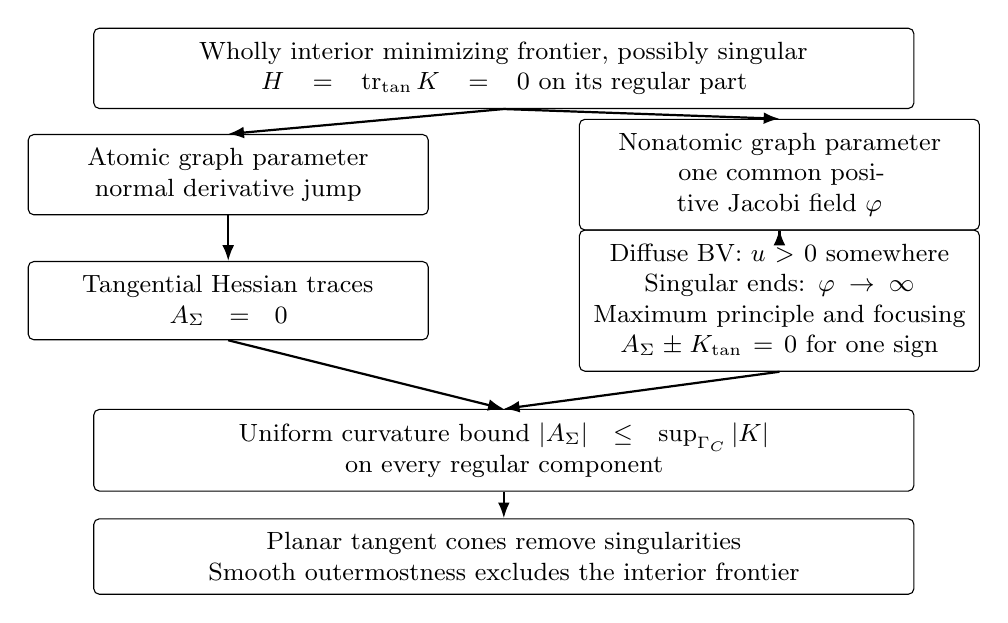
\begin{tikzpicture}[
 box/.style={draw,rounded corners=2pt,align=center,font=\small,
             inner sep=5pt,text width=.39\linewidth},
 flow/.style={-{Latex[length=2mm]},thick}]
 \node[box,text width=.83\linewidth] (family) at (0,0)
   {Wholly interior minimizing frontier, possibly singular\\
    $H=\tr_{\rm tan}K=0$ on its regular part};
 \node[box] (atom) at (-3.5,-1.35)
   {Atomic graph parameter\\
    normal derivative jump};
 \node[box] (nonatomic) at (3.5,-1.35)
   {Nonatomic graph parameter\\
    one common positive Jacobi field $\varphi$};
 \node[box] (flat) at (-3.5,-2.95)
   {Tangential Hessian traces\\
    $A_\Sigma=0$};
 \node[box] (maximum) at (3.5,-2.95)
   {Diffuse BV: $u>0$ somewhere\\
    Singular ends: $\varphi\to\infty$\\
    Maximum principle and focusing\\
    $A_\Sigma\pm K_{\rm tan}=0$ for one sign};
 \node[box,text width=.83\linewidth] (bound) at (0,-4.85)
   {Uniform curvature bound $|A_\Sigma|\le\sup_{\Gamma_C}|K|$\\
    on every regular component};
 \node[box,text width=.83\linewidth] (finish) at (0,-6.2)
   {Planar tangent cones remove singularities\\
    Smooth outermostness excludes the interior frontier};
 \draw[flow] (family.south) -- (atom.north);
 \draw[flow] (family.south) -- (nonatomic.north);
 \draw[flow] (atom) -- (flat);
 \draw[flow] (nonatomic) -- (maximum);
 \draw[flow] (flat.south) -- (bound.north);
 \draw[flow] (maximum.south) -- (bound.north);
 \draw[flow] (bound) -- (finish);
\end{tikzpicture}
\caption{Removal of singular frontiers carrying area mass. Each regular
component follows one of the two routes. The common curvature bound holds
for one full-measure family of minimizers, after the countable
exceptional-family step in
Theorem~\ref{thm:variation:boundary-support}.}
\label{fig:variation:singular-localization}
\end{figure}

\begin{lemma}[Atoms give totally geodesic sheets]\label{lem:variation:atomic-flatness}
Fix a uniform graph cylinder about a free regular sheet $\Sigma$ of a
minimizer.  Collapse coincident graphs and parametrize the remaining
graphs by their height at a fixed base point.  If the parameter of
$\Sigma$ has positive mass under the pushforward of $\pi$, then the
second fundamental form $A_\Sigma$ vanishes on its smaller patch.
\end{lemma}

\begin{proof}
Use Fermi coordinates $(y,s)$ about the smooth reference sheet, with
$g=ds^2+g_s$, $s=0$ on $\Sigma$, and
$A_{ab}=\tfrac12\partial_s(g_s)_{ab}$.  Let $a>0$ be the mass of the
coincident-graph fiber.  Its contribution to
Equation~\eqref{eq:variation:hessian} is
$(ca/2)\,ds\otimes ds\,dA_\Sigma$.
In the $ss$ equation this is the density $(ca/2)\delta_0(ds)$ on
almost every normal line; the volume and surface densities coincide
at $s=0$.  All other graph parameters have height different from zero
on every such line, by noncrossing and contact agreement.  They
contribute no atom at zero.  Semiconvexity and local Lipschitz bounds
give bounded one-sided traces of $\partial_su$ on almost every line,
and slicing the equation proves
\begin{equation}\label{eq:variation:normal-jump}
 (\partial_su)^+-(\partial_su)^-=ca/2.
\end{equation}

The tangential equations contain no jump measure on the reference
sheet.  Contributions from nearby sheets must also be controlled
before taking traces.  Equation~\eqref{eq:variation:graph-separation} implies that a nearby leaf at
distance $|s|$ has tangential normal components $O(|s|)$ relative to
the reference Fermi frame, on a smaller patch.  Indeed Harnack
compares its height at the fixed base point to its height at the
chosen point, and the derivative estimate controls its tilt.  Thus
the tangential--tangential components of $d\mathcal N$ in
$|s|<\varepsilon$ have total variation bounded by
$C\varepsilon^2\sigma(\{|s|<\varepsilon\})$.  After division by the
slab width this tends to zero; the total local $\sigma$ mass is
bounded.  This estimate also covers infinitely many accumulating
leaves and their diffuse parameter measure.

Average the tangential equation over $0<s<\varepsilon$ and over
$-\varepsilon<s<0$, and test in the $y$ variables.  The continuous
tensor $\mathcal B(u,X,\nabla X)$ has identical limiting traces.  On
each parallel sheet,
\[
 (\Hess_g u)_{ab}=(\Hess_{g_s}u|_{s})_{ab}
                              +A_{ab}(s)\partial_su.
\]
Uniform continuity of $u$ makes the two averaged intrinsic Hessians
converge to the same distribution, and the bounded normal derivatives
converge to their one-sided traces in $L^1$ on smaller base patches.
Taking the difference and using the vanishing measure contribution
therefore gives $A_{ab}(0)[\partial_su]=0$ as distributions.  Equation~\eqref{eq:variation:normal-jump} and smoothness of $A$ prove $A=0$.
\end{proof}

\subsection{Jacobi fields from neighboring minimizers}

On a free sheet with Equation~\eqref{eq:variation:three-equations}, let $L_0$
be the minimal Jacobi operator and $L_\pm$ the normal linearizations of
$H\pm\tr_{\rm tan}K$.  Explicitly,
\begin{align}
 L_0f&=-\Delta_\Sigma f-(|A_\Sigma|^2+\Ric(\nu,\nu))f,
 \label{eq:variation:L0}\\
 L_\pm f&=L_0f\ \pm2K(\nu,\nabla_\Sigma f)
                      \pm\tr_{T\Sigma}(\nabla_\nu K)f.
 \label{eq:variation:Lpm}
\end{align}
These formulas follow from $\nu'=-\nabla_\Sigma f$ and the
mean-curvature variation formula.  In the trace of $K$, the two terms
from differentiating the tangent frame cancel the variation of the
inverse induced metric, leaving precisely the last two terms above.

\begin{lemma}[One common positive Jacobi field]
\label{lem:variation:common-jacobi}
Let $C\in\supp\pi$ belong to the full-measure family in
Lemma~\ref{lem:variation:contact-dichotomy}, with wholly interior
frontier, and let $\Sigma$ be a connected component of its regular
part.  If its local graph parameter at some patch is not an atom,
there is a smooth positive function $\varphi$ on all of $\Sigma$ with
\begin{equation}\label{eq:variation:common-jacobi}
 L_0\varphi=L_+\varphi=L_-\varphi=0.
\end{equation}
\end{lemma}

\begin{proof}
Fix a base point $y_0$ in the patch.  The fiber of minimizers whose
graph agrees there has $\pi$ measure zero.  Every neighborhood of $C$
in the compact metric space $\mathfrak T$ has positive $\pi$ measure.
Deleting this fiber and the exceptional family from
Lemma~\ref{lem:variation:contact-dichotomy}, choose $C_j\to C$ with
distinct graphs at $y_0$, all satisfying
Equation~\eqref{eq:variation:three-equations} near the component.

Choose a connected relatively compact smooth exhaustion of $\Sigma$
by domains containing $y_0$.  For each fixed exhaustion domain,
multiplicity-one regular convergence and finitely many overlapping
graph charts express $\Gamma_{C_j}$ as one smooth normal graph $h_j$
over it, with $h_j\to0$ smoothly.  Noncrossing says this graph either
agrees with $\Sigma$ or is strictly on one side.  Agreement at one
point propagates through overlapping charts by strong comparison;
it would contradict distinction at $y_0$.  A subsequence thus has a
fixed strict sign on every exhaustion domain.

Divide $h_j$ by its signed value at $y_0$, obtaining positive functions
normalized to one there.  Each satisfies the linear difference
equation for the two minimal graphs.  The coefficients converge
smoothly to those of $L_0$.  Harnack along a finite chain of balls
and interior estimates bound the normalized graphs and all their
derivatives on each compact subset.  Diagonal extraction gives a
smooth positive limit $\varphi$ on all of $\Sigma$.  The same graph
differences solve the two difference equations for
$H\pm\tr_{\rm tan}K=0$; their coefficients converge to $L_\pm$.
Passing to the same limit proves all three equations in
Equation~\eqref{eq:variation:common-jacobi}.  This argument requires a sequence
of neighboring minimizers, not a differentiable family.
\end{proof}


\subsection{Focusing and the positive stress measure}

The common Jacobi field will provide the comparison function for a
maximum principle. We now establish the inequality it will be compared
with. The positive Hessian source in the lapse equation becomes a
positive spatial stress after trace reversal; retaining that source is
what gives the favorable sign in the focusing inequality.


\begin{lemma}[The stationary metric adjoint]
\label{lem:variation:stationary-action}
Let $u>0$ and $X$ be smooth on an open set with smooth metric $g$, and put
\[
 \mathbf g=-u^2dz^2+g_{ij}(dx^i+X^i dz)(dx^j+X^j dz),
 \qquad b=-u^{-1}\operatorname{sym}\nabla X.
\]
Let $\mu_b,J_b$ be the constraints of $(g,b)$, and let $S_b$ denote
the expression $\mathcal S$ in Equation~\eqref{eq:variation:S}, with
$K$ replaced throughout by $b$.  Then the exact smooth identity is
\[
 \nabla^2u-(\Delta u)g+S_b
  =-u\mathbf G_{\mathrm{spatial}}
        -(u\mu_b+J_b(X))g-(J_b)_{(i}X_{j)}.
\]
Here the spatial Einstein tensor is its restriction to the tangent
spaces of $z=\mathrm{constant}$, and parentheses include the factor
$1/2$.
\end{lemma}

\begin{proof}
All variations and integrations in this proof have compact support in
the open set.  Define
\[
 \mathsf B(B,C)=\langle B,C\rangle_g
                    -(\operatorname{tr}_gB)(\operatorname{tr}_gC).
\]
Temporarily let $K$ be independent of the metric.  Integration of the
momentum divergence, at fixed contravariant shift $X$, gives
\[
 \begin{split}
 \int(2u\mu+2J(X))\,dV_g
 &=\int u\{R_g-\mathsf B(K,K)+2\mathsf B(K,b)\}\,dV_g\\
 &=\int u\{R_g+\mathsf B(b,b)
                  -\mathsf B(K-b,K-b)\}\,dV_g.
 \end{split}
\]
At $K=b$ the final square has zero first variation, including for a
metric variation with the covariant components of $K$ held fixed.
Thus the metric derivative of the constraint functional at this point
equals that of the stationary scalar action
$\int u(R_g+\mathsf B(b,b))\,dV_g$.

For completeness, its relation to the spacetime scalar action follows
from the Gaussian contraction formulas with lapse and shift.  They
give
\[
 \mathbf R=R_g+|b|^2+(\operatorname{tr}b)^2
       +2\mathbf n(\operatorname{tr}b)-2u^{-1}\Delta u.
\]
Stationarity implies
$\mathbf n(\operatorname{tr}b)=-u^{-1}X(\operatorname{tr}b)$ and
$\operatorname{div}X=-u\operatorname{tr}b$, whence
\[
 \mathbf R=R_g+\mathsf B(b,b)
        -2u^{-1}\operatorname{div}
                    \bigl(\nabla u+(\operatorname{tr}b)X\bigr).
\]
Since $\sqrt{|\det\mathbf g|}=u\sqrt{\det g}$, the two scalar actions
differ by a spatial divergence per unit $z$-length.  For a spacetime
metric variation $H$, differentiating the connection formula for
scalar curvature gives
\[
 \delta(\mathbf R\,dV_{\mathbf g})
   =\left[-\langle\mathbf G,H\rangle_{\mathbf g}
    +\boldsymbol\nabla_\alpha
       \bigl(\boldsymbol\nabla_\beta H^{\alpha\beta}
              -\boldsymbol\nabla^\alpha\operatorname{tr}_{\mathbf g}H
       \bigr)\right]dV_{\mathbf g}.
\]
At fixed $u,X$, $H=h_{ij}(dx^i+X^i dz)(dx^j+X^j dz)$ annihilates the
unit normal in each slot.  The derivative of the stationary action
therefore pairs $h$ with $-u\mathbf G_{\mathrm{spatial}}$.

The metric coefficient of the constraint integral before ray
transport is
\[
 \nabla^2u-(\Delta u)g+S_b+(J_b)_{(i}X_{j)}
                   +(u\mu_b+J_b(X))g.
\]
The last term is the volume derivative, and the preceding added term
restores the term removed by isometric ray transport in the
definition of $S_b$.  Equating the two coefficients proves the
identity.  This also displays why the volume derivative disappears
only after complementarity has been imposed.
\end{proof}

\begin{lemma}[Focusing with a positive Hessian measure]
\label{lem:variation:measure-focusing}
Let $g,K$ be smooth on $U$, with $\mu\geq|J|_g$.  Suppose that $u$ is
locally Lipschitz and semiconvex, $X\in C^{1,1}_{\mathrm{loc}}$, and
the following exact distributional equations hold:
\[
 \begin{gathered}
 u\geq|X|_g,\qquad u\mu+J(X)=0,\qquad
 \operatorname{sym}\nabla X=-uK,\\
 \nabla^2u=-S+\frac{\operatorname{tr}_gS}{n-1}g+\mathcal M,
 \end{gathered}
\]
where
\[
 \begin{split}
 S={}&-u\operatorname{Ric}_g+2u(K^2-\tau K)
        +\mathcal L_XK-(\operatorname{div}X)K\\
     &-\operatorname{div}(K(X,\cdot))g-J_{(i}X_{j)},
 \end{split}
\]
and $\mathcal M$ is a locally finite positive semidefinite symmetric
tensor measure, interpreted relative to $dV_g$.  In the application,
\[
 \mathcal M=\frac c2\int\nu_D^\flat\otimes\nu_D^\flat\,dA_D\,d\pi.
\]
Let $\Sigma\subset U$ be a smooth two-sided hypersurface with
$H_\Sigma=\operatorname{tr}_\Sigma K=0$, and let $\nu$ be its chosen
unit normal.  Set
\[
 \begin{split}
 L_\pm f={}&-\Delta_\Sigma f
        \pm2K(\nu,\nabla_\Sigma f)\\
 &+\bigl[-|A_\Sigma|^2-\operatorname{Ric}_g(\nu,\nu)
                 \pm\operatorname{tr}_\Sigma(\nabla_\nu K)\bigr]f,
 \qquad Q_\pm=u\mp g(X,\nu).
 \end{split}
\]
Then $Q_\pm\geq0$, and, on the open subset $\Sigma\cap\{u>0\}$,
\[
 L_\pm Q_\pm\leq-u|A_\Sigma\pm K_{\mathrm{tan}}|^2
\]
in distributions.  Precisely, each inequality holds after pairing
with any nonnegative smooth compactly supported test function on
that open subset.
\end{lemma}

\begin{proof}
The operator formula follows by varying $\Sigma$ with velocity $f\nu$.
The mean-curvature derivative is
$-\Delta_\Sigma f-(|A_\Sigma|^2+\operatorname{Ric}_g(\nu,\nu))f$.
For the other term, differentiation of
$\operatorname{tr}_\Sigma K=\operatorname{tr}_gK-K(\nu,\nu)$, using
$\dot\nu=-\nabla_\Sigma f$, gives
$f\operatorname{tr}_\Sigma(\nabla_\nu K)
 +2K(\nu,\nabla_\Sigma f)$.  Adding the two derivatives gives $L_+$;
replacing $K$ by $-K$ gives $L_-$.

Fix a compact patch of $\Sigma\cap\{u>0\}$.  Enlarge it slightly to
a coordinate neighborhood on which $u\geq a>0$.  All constants below
may depend on this neighborhood, $a$, the smooth data, and the stated
local Lipschitz bounds; the only limiting parameter is the mollifier
radius $\varepsilon\downarrow0$.  Choose a nonnegative smooth
convolution kernel of integral one.  Mollify $u$ and the components
of the covector $w=X^\flat$, and then put
\[
 u_\varepsilon=u*\rho_\varepsilon,\qquad
 w_\varepsilon=w*\rho_\varepsilon,\qquad
 X_\varepsilon=g^{-1}w_\varepsilon,
 \qquad b_\varepsilon=-u_\varepsilon^{-1}
                    \operatorname{sym}\nabla X_\varepsilon.
\]
Convolutions are used only on smaller coordinate neighborhoods.
In particular $u_\varepsilon\geq a/2$ for small $\varepsilon$.

We need convergence of $b_\varepsilon$ through one derivative.
For a smooth coefficient $a_0$ and a Lipschitz function $f$, let
\[
 C_\varepsilon(a_0,f)=(a_0f)*\rho_\varepsilon
                              -a_0(f*\rho_\varepsilon).
\]
The integral formula with integrand
$(a_0(y)-a_0(x))f(y)\rho_\varepsilon(x-y)$ gives
$\|C_\varepsilon(a_0,f)\|_\infty\leq C\varepsilon\|f\|_\infty$.
Differentiation in distributions gives the useful identity
\[
 \partial_j C_\varepsilon(a_0,f)
    =C_\varepsilon(\partial_j a_0,f)
                         +C_\varepsilon(a_0,\partial_jf).
\]
The same integral bound, applied to the bounded weak derivative of
$f$, proves
\[
 \|C_\varepsilon(a_0,f)\|_{C^1}
       \leq C\varepsilon\|f\|_{W^{1,\infty}}.
\]
In covector coordinates the shift equation reads
$\tfrac12(\partial_iw_j+\partial_jw_i)-\Gamma^l_{ij}w_l=-uK_{ij}$.
Thus
\[
 \operatorname{sym}\nabla X_\varepsilon+u_\varepsilon K
   =C_\varepsilon(\Gamma,w)-C_\varepsilon(K,u)=O_{C^1}(\varepsilon).
\]
The positive lower bound for $u_\varepsilon$ and its bounded first
derivatives therefore give
\[
 b_\varepsilon\longrightarrow K\quad\hbox{in }C^1.
\]
Also $X_\varepsilon\to X$ in $C^1$, $u_\varepsilon\to u$ uniformly,
and all their first derivatives are uniformly bounded.

Put $B=-S+(\operatorname{tr}_gS)g/(n-1)$; it is continuous under the
stated regularity.  To convolve the tensor measure precisely, write
$dV_g=v_g\,dx$ in the chosen chart and convolve the component measures
$v_g^{-1}\,d\mathcal M_{ij}$.  Denote the resulting matrix of smooth
functions by $M_\varepsilon$.  This matrix is positive semidefinite at
each point, because the convolution kernel and $v_g^{-1}$ are
nonnegative.  The Hessian equation and the connection commutator give
\[
 \nabla^2u_\varepsilon=B*\rho_\varepsilon
                            +M_\varepsilon+o_{C^0}(1).
\]
Indeed the sole extra term is
$(\Gamma\,du)*\rho_\varepsilon-\Gamma\,d u_\varepsilon$, which is
$O(\varepsilon)$ since $du$ is bounded.  No derivative of $du$ is
required in this estimate.

Define the stationary smooth spacetime metric from
$u_\varepsilon,X_\varepsilon,g$ as in
Lemma~\ref{lem:variation:stationary-action}.  Its induced second form is
$b_\varepsilon$; let $\mu_\varepsilon,J_\varepsilon$ be its constraint
components.  Since $b_\varepsilon\to K$ in $C^1$,
\[
 \mu_\varepsilon\to\mu,\qquad J_\varepsilon\to J,\qquad
 S_{b_\varepsilon}(u_\varepsilon,X_\varepsilon)\to S
\]
uniformly.  The smooth action identity and the convolved Hessian
equation consequently give
\[
 u_\varepsilon\mathbf G^\varepsilon_{\mathrm{spatial}}
   =P_\varepsilon-J_{(i}X_{j)}+o_{C^0}(1),\qquad
 P_\varepsilon=(\operatorname{tr}_{g(x)}M_\varepsilon)g(x)
                                                     -M_\varepsilon.
\]
Here the regular terms cancel because
$B-(\operatorname{tr}_gB)g+S=0$, and the volume term tends to zero by
$u\mu+J(X)=0$.  The matrix $P_\varepsilon$ is positive semidefinite:
in a $g(x)$-orthonormal eigenbasis for $M_\varepsilon$ its eigenvalues
are the sums of all but one of the nonnegative eigenvalues of
$M_\varepsilon$.  It is essential that this trace reversal be applied
\emph{after} convolution, at $g(x)$.  There is no estimate here
commuting a variable trace-reversal coefficient past an unbounded
Hessian.  For the area measure in the statement, the corresponding
unmollified positive spatial measure is exactly
\[
 \frac c2\int(g-\nu_D^\flat\otimes\nu_D^\flat)\,dA_D\,d\pi.
\]

Let $\mathbf n_\varepsilon$ be the future slice normal.  For the
$g$-unit normal $\nu$ of $\Sigma$, Gauss--Codazzi and nullness yield
\[
 \begin{split}
 u_\varepsilon\mathbf{Ric}^\varepsilon
       (\mathbf n_\varepsilon\pm\nu,
        \mathbf n_\varepsilon\pm\nu)
 &=u_\varepsilon\mathbf G^\varepsilon
       (\mathbf n_\varepsilon\pm\nu,
        \mathbf n_\varepsilon\pm\nu)\\
 &\geq u\mu\pm2uJ(\nu)-J(\nu)g(X,\nu)-o(1)\geq-o(1).
 \end{split}
\]
To check the last inequality pointwise, if $\mu=0$ then $J=0$.
Otherwise complementarity and $u\geq|X|$ imply
$|J|=\mu$, $|X|=u$, and $J=-\mu X^\flat/u$.  The expression is
therefore $u\mu(1\pm J(\nu)/\mu)^2$.  This verifies the null Ricci
lower bound uniformly, without bounding $M_\varepsilon$ or the full
spacetime curvature.

We give the smooth focusing identity used to finish.  Write
$\theta_\varepsilon=H_\Sigma+\operatorname{tr}_\Sigma b_\varepsilon$
and $\ell_\varepsilon=\mathbf n_\varepsilon+\nu$.  Launch orthogonal
null geodesics from the patch, and intersect their local null
hypersurface with the stationary slices.  For each fixed
$\varepsilon$ this is a smooth construction for some positive time;
no uniform time interval is needed.  On each slice normalize the
null generator by $\ell=\mathbf n+\nu$.  If $\chi$ denotes its screen
second form, commuting covariant derivatives along an affinely
parametrized generator in a parallel screen frame gives
\[
 \nabla_\ell\chi_{ab}=-\chi_{ac}\chi_{cb}-\mathcal R_{ab},
 \qquad \sum_a\mathcal R_{aa}=\mathbf{Ric}(\ell,\ell),
\]
where $\mathcal R$ is the screen Jacobi curvature matrix.
Tracing gives $\ell(\theta)=-|\chi|^2-\mathbf{Ric}(\ell,\ell)$ for
that affine normalization.  For the slice normalization,
$\boldsymbol\nabla_\ell\ell=\kappa\ell$, so the trace identity instead
has the additional term $\kappa\theta$.  Differentiating
$\mathbf g(\ell,\mathbf n)=-1$ gives
\[
 \kappa=\mathbf g(\ell,\boldsymbol\nabla_\ell\mathbf n)
          =u^{-1}\nu(u)+b(\nu,\nu),
\]
because the slice-normal acceleration is $\nabla\log u$.

The velocity with slice coordinate $z$ as parameter is $u\ell$.
Subtracting the stationary Killing translation
$\partial_z=u\mathbf n+X$ leaves the spatial velocity $u\nu-X$,
whose normal component is $Q=u-X\cdot\nu$ and tangential component
is $-X^T$.  At the initial slice $\chi=A_\Sigma+b|_{T\Sigma}$.
Thus the two descriptions of the expansion derivative give exactly
\[
 \begin{split}
 L_{+,\varepsilon}Q_{+,\varepsilon}
       -X_\varepsilon^T(\theta_\varepsilon)
  ={}&-u_\varepsilon\bigl(
       |A_\Sigma+(b_\varepsilon)_{\mathrm{tan}}|^2
       +\mathbf{Ric}^\varepsilon(\ell_\varepsilon,
                                  \ell_\varepsilon)\bigr)\\
    &+\bigl(\nu(u_\varepsilon)
              +u_\varepsilon b_\varepsilon(\nu,\nu)\bigr)
                                                    \theta_\varepsilon.
 \end{split}
\]
The notation $L_{+,\varepsilon}$ means the displayed spatial
linearization with $K$ replaced by $b_\varepsilon$, without assuming
that $\theta_\varepsilon$ is zero.

Since $H_\Sigma=\operatorname{tr}_\Sigma K=0$ and
$b_\varepsilon\to K$ in $C^1$, one has
$\theta_\varepsilon\to0$ in $C^1$ on the patch.  Both the tangential
transport term and the final normalization term therefore tend
uniformly to zero; their coefficients involve only bounded first
jets.  The null Ricci lower bound gives
\[
 L_{+,\varepsilon}Q_{+,\varepsilon}
       \leq-u_\varepsilon
                 |A_\Sigma+(b_\varepsilon)_{\mathrm{tan}}|^2+o(1).
\]
The principal part of all these operators is the fixed
$-\Delta_\Sigma$.  Their first-order and zeroth-order coefficients
converge uniformly, while $Q_{+,\varepsilon}\to Q_+$ uniformly with
uniform local Lipschitz bounds.  Pairing with a compactly supported
smooth test function and integrating the Laplacian by parts thus
passes to the asserted distributional inequality.  For the drift
term, the gradients converge weakly against integrable test fields,
and the error in its coefficient tends uniformly to zero.

Finally replace stationary time $z$ by $-z$ and the future normal by
its negative.  This replaces $(K,X,J)$ by $(-K,-X,-J)$ while leaving
$u,g,S,B,\mathcal M$ unchanged.  Applying the plus calculation gives
$Q_-=u+X\cdot\nu$ and the claimed minus inequality.  The argument is
local on every compact subset of $\{u>0\}$, so a partition of unity
establishes the statement for all test functions specified in the
lemma.
\end{proof}

\subsection{Capacity estimates and positive Jacobi fields at singular ends}

The maximum-principle argument will be applied to $Q_\pm/\varphi$.
To ensure that a positive maximum cannot escape into the singular
set, we prove that $1/\varphi$ is bounded and tends to zero there.
Capacity cutoffs allow bounded subsolutions to cross the singular
set; dilation and a cone Liouville theorem then give the required
vanishing along every singular approach.

We first specify the geometric measure theory used in this subsection.
Let $\Gamma$ be the compact support of the perimeter measure of a set
whose boundary is locally perimeter minimizing in an open subset of a
smooth $(k+1)$-dimensional Riemannian manifold.  The open subset contains
$\Gamma$; thus there is no boundary condition or obstacle in this
subsection.  Write $\mathcal S=\operatorname{sing}\Gamma$ and
$d\mu=d\mathcal H^k_g\lfloor\Gamma$.
The interior regularity, monotonicity, and compactness theorems for
minimizing boundaries give the following facts \cite{Simon2018}:
$\Gamma\setminus\mathcal S$ is a smooth embedded minimal hypersurface,
$\mathcal S$ is closed with Hausdorff dimension at most $k-7$, and
$\mu(B_r(x))\leq\Lambda r^k$ for $x\in\Gamma$ and all sufficiently small
$r$, with uniform constants on the compact ambient neighborhood.
The singular set is empty when $k\leq6$.
Dilations about a fixed point have subsequences converging to
multiplicity-one perimeter-minimizing boundary cones, with convergence
of perimeter measures and supports on compact sets, and smooth
multiplicity-one graphical convergence on compact subsets of the
regular limit.  A multiplicity-one plane tangent cone implies
regularity of the original point.  These statements concern boundaries
of sets; no multiplicity assumption is being inferred merely from
stationarity of a varifold.

\begin{lemma}[Removal of the singular set for bounded subsolutions]
\label{lem:variation:capacity-submean}
Suppose $k>2$ and let $\Gamma$ be as above.  A bounded nonnegative
function $w\in W^{1,2}_{\mathrm{loc}}(\Gamma\setminus\mathcal S)$
satisfying $\Delta_\Gamma w\geq-F$ weakly there, where $F\geq0$ is
constant, has locally finite Dirichlet energy through $\mathcal S$.
The inequality extends to compactly supported tests on all of
$\Gamma$.  There are $r_0>0$ and $C_0<\infty$, depending only on the
ambient neighborhood, $k$, and $\Lambda$, such that
\[
 \mathop{\rm ess\,sup}_{\Gamma\cap B_{r/2}(x)} w
 \leq C_0\left[
       \left(r^{-k}\int_{\Gamma\cap B_r(x)}w^2\,d\mu\right)^{1/2}
       +Fr^2\right],\qquad 0<r\leq r_0.
\]
For a continuous function on the regular part the essential supremum
can be replaced by the supremum there.  The constants are uniform
under dilations by scales tending to zero about points in the fixed
compact ambient neighborhood.  One may in particular start with $w$
on one regular component and extend it by zero to the other regular
components.
\end{lemma}

\begin{proof}
Here is the capacity calculation and the energy argument needed before
using a Sobolev inequality.  On a fixed compact region cover its
singular set by finitely many ambient balls $B_{r_i}(p_i)$, with
$r_i<\varepsilon$ and $\sum_i r_i^{k-2}<\varepsilon$.
Such covers exist because
$\dim_{\mathcal H}\mathcal S\leq k-7<k-2$.
Let $\theta_i$ be one on $B_{r_i}(p_i)$, zero outside $B_{2r_i}(p_i)$,
and satisfy $|\nabla\theta_i|\leq2/r_i$.
The cutoff $\chi=1-\max_i\theta_i$ satisfies
\[
 \int_\Gamma|\nabla\chi|^2\,d\mu
 \leq C\Lambda\sum_i r_i^{k-2},\qquad
 \int_\Gamma(1-\chi)^2\,d\mu
 \leq C\Lambda\sum_i r_i^k.
\]
The first estimate follows pointwise almost everywhere by selecting an
index attaining the maximum.  Taking shrinking covers gives
$0\leq\chi_j\leq1$, equal to zero near $\mathcal S$, converging to one
at every regular point, with both displayed integrals tending to zero.
Local versions use a slightly larger compact region than the support
of the test under consideration.

For a fixed smooth ambient cutoff $\eta$, test the subsolution
inequality with $\eta^2\chi_j^2w$.  Sobolev approximation on the smooth
regular part justifies this test.  Expanding and applying Young's
inequality gives
\[
 \int \eta^2\chi_j^2|\nabla w|^2\,d\mu
 \leq 4\int w^2|\nabla(\eta\chi_j)|^2\,d\mu
      +2F\int\eta^2\chi_j^2w\,d\mu.
\]
The right side is uniformly bounded because $w$ is bounded, the area
is locally finite, and the capacity energies tend to zero.  Fatou's
lemma proves local finite energy.  Moreover, $\chi_jw$ converges to
$w$ in local $W^{1,2}$: the extra gradient $w\nabla\chi_j$ tends to
zero in $L^2$, and dominated convergence applies to
$(1-\chi_j)\nabla w$.
For a nonnegative smooth compact test $\psi$, the tests
$\psi\chi_j^2$ now pass to the limit in the weak inequality.  Indeed,
the only extra term is bounded by
\[
 2\|\psi\|_\infty
 \|\nabla w\|_{L^2(\operatorname{supp}\psi)}
 \|\nabla\chi_j\|_{L^2},
\]
and tends to zero.  This proves removability, without assuming energy
regularity in advance.

The required Sobolev input is the Michael--Simon inequality
\cite{MichaelSimon1973}, in the following local $L^2$ form:
\[
 \left(\int|v|^{2k/(k-2)}\,d\mu\right)^{(k-2)/k}
 \leq C\int\bigl(|\nabla v|^2+C_{\mathrm{amb}}v^2\bigr)\,d\mu.
\]
Initially $v$ is compactly supported in the regular part.  To obtain
this form, apply the $L^1$ Michael--Simon inequality to
$|v|^{2(k-1)/(k-2)}$ and use Cauchy--Schwarz.  A smooth isometric
embedding of a slightly larger compact ambient neighborhood gives a
bound for its second fundamental form.  Since $\Gamma$ is minimal
in the ambient metric, its Euclidean mean curvature in that embedding
is bounded by the trace of this ambient second fundamental form.
In particular the bound does not involve $|A_\Gamma|$.
The capacity approximation just proved extends the inequality to the
tests used here.  Dilating this fixed embedding multiplies its
second fundamental form by the dilation scale, which also proves the
claimed uniformity in blow-ups.

For completeness, put $v=w+Fr^2$; if $F=0$, first put $v=w+\delta$
and later let $\delta\downarrow0$.  On $B_r(x)$ this is a positive
subsolution of $\Delta v\geq-r^{-2}v$.
Testing with $\eta^2v^{p-1}$, $p\geq2$, and applying the preceding
Sobolev inequality gives
\[
 \left(\int|\eta v^{p/2}|^{2k/(k-2)}\,d\mu\right)^{(k-2)/k}
 \leq Cp^2\int
       (|\nabla\eta|^2+r^{-2}\eta^2)v^p\,d\mu,
\]
after decreasing $r_0$ so the bounded ambient term is absorbed in
$r^{-2}$.  All power tests follow from boundedness of $w$ and the
energy approximation above.  Iteration with
$p_j=2(k/(k-2))^j$ on radii
$r/2+r/2^{j+1}$ yields the displayed submean estimate; the factors
converge since $\sum_j(1+j)/p_j<\infty$.
The contribution of the added constant is bounded by $CFr^2$ using
$\mu(B_r)\leq\Lambda r^k$.
Finally, every regular point has a connected smooth neighborhood in
one regular component.  The boundary within $\Gamma$ of any regular
component is contained in $\mathcal S$.  Zero extension to other
components therefore adds no regular interface, and the same
capacity argument applies.
\end{proof}

\begin{lemma}[A flat link component determines the entire cone]
\label{lem:variation:flat-link-component}
Let $C\subset\mathbb R^{k+1}$ be the support of a nonzero
multiplicity-one perimeter-minimizing boundary cone.  If a component
of the regular link $L_{\mathrm{reg}}=(C\cap S^k)_{\mathrm{reg}}$
is totally geodesic in $S^k$, then $C$ is a hyperplane.
\end{lemma}

\begin{proof}
Write $d=k-1$ for the link dimension and
$\mathcal S_L=(\operatorname{sing}C)\cap S^k$.
The product description of the cone away from its vertex and the
singular-dimension estimate give
$\dim_{\mathcal H}\mathcal S_L\leq k-8=d-7$ when the link is
singular.  Its area growth is of order $r^d$: on a fixed annulus the
radial product formula and cone area growth imply this bound by
integrating over radial intervals of length comparable to $r$.
Thus $\mathcal S_L$ has zero $2$-capacity in the link by the preceding
cover construction.  A smooth link needs no capacity cutoffs.

Let $U$ be the totally geodesic regular component.  It lies in a
great equator $E$ and is open in $E$.  Every limit point of $U$ that
is regular belongs to $U$: a connected local regular chart through
that point meets $U$, so belongs to the same component.  Consequently
$U$ is relatively closed as well as open in $E\setminus\mathcal S_L$.
This latter set is connected.  One elementary justification is to
use stereographic coordinates on $E$.  Given two points outside
$\mathcal S_L$, almost every intermediate point can be joined to both
by straight segments missing $\mathcal S_L$: the set of bad
intermediate points is contained in the two radial shadows of that
set, whose Hausdorff dimension is at most
$\dim_{\mathcal H}\mathcal S_L+1<d$.  Taking countably many bounded
pieces handles the point omitted by stereographic projection.
Thus $U=E\setminus\mathcal S_L$, and closedness of the support implies
$E\subset C\cap S^k$.

Any other connected regular link component $V$ is disjoint from $E$.
Indeed a smooth regular neighborhood of a point of $E$ already
contains the equatorial sheet; as an embedded hypersurface of the
same dimension it is that sheet locally.  By connectedness $V$ lies
in one strict hemisphere.  Its suitably signed equatorial height
$h$ satisfies
\[
 h>0,\qquad |h|\leq1,\qquad |\nabla_Vh|\leq1,
 \qquad \Delta_Vh=-d h.
\]
This Laplace identity holds for coordinate functions on a minimal
$d$-dimensional submanifold of the unit sphere.
Test it on $V$ with the squared link capacity cutoffs $\chi_j^2$.
These tests have compact support in $V$: any relative boundary of
$V$ in the compact link is singular.  They give
\[
 d\int_Vh\chi_j^2\,d\mathcal H^d
 =2\int_V\chi_j\langle\nabla h,\nabla\chi_j\rangle\,d\mathcal H^d
 \longrightarrow0.
\]
Here Cauchy--Schwarz, the finite link area, and the vanishing
capacity energy justify the limit.  Dominated convergence gives
$\int_Vh=0$, contradicting $h>0$ on a nonempty open component.
Hence no such $V$ exists.  The regular support is contained in $E$;
the singular set has zero link area, and the regular set is dense in
the support.  Thus the support is precisely $E$, and multiplicity
one makes the cone a hyperplane.
\end{proof}

\begin{lemma}[A Liouville theorem for minimizing cones]
\label{lem:variation:cone-liouville}
Let $C$ be a nonflat multiplicity-one perimeter-minimizing boundary
cone of dimension $k$.  If $z$ is a bounded, nonnegative, smooth
function on $\operatorname{reg}C$ satisfying
\[
 \Delta_C z\geq |A_C|^2z,
\]
then $z=0$.  No smoothness or connectedness of the regular link is
assumed.
\end{lemma}

\begin{proof}
A nonflat minimizing boundary cone has $k\geq7$.
In logarithmic radius $s=\log r$ and the regular link $L$, set
$a=k-2>0$, $V=|A_L|^2$, and $Z(s,\omega)=z(e^s\omega)$.
The cone metric and the scaling of the second fundamental form give
\[
 Z_{ss}+aZ_s+\Delta_L Z\geq VZ.
\]
The operator on the left is in divergence form for the measure
$e^{as}\,ds\,d\mathcal H^{k-1}_L$.
On any compact $s$-strip, test after dropping $VZ\geq0$ with
$\eta(s)^2\chi_j(\omega)^2 Z$.
The energy proof in Lemma~\ref{lem:variation:capacity-submean}, with
this smooth positive weight, proves finite energy on smaller strips
and permits removal of the link capacity cutoffs.  In particular,
tests constant in the link variable are legitimate.  It follows that
\[
 q(s)=\int_LZ(s,\omega)\,d\mathcal H^{k-1}_L(\omega)
 \quad\hbox{satisfies}\quad q''+a q'\geq0
\]
on the entire real line in distributions.  The energy bound gives
$q\in H^1_{\mathrm{loc}}(\mathbb R)$, so we use its continuous
representative.  It is bounded and nonnegative.

Such a $q$ is nondecreasing.  To see this, convolve with a smooth
nonnegative kernel.  For the resulting smooth bounded function,
$(e^{as}q')'\geq0$.  If $q'(s_0)<0$, then for every $s<s_0$
\[
 q'(s)\leq e^{a(s_0-s)}q'(s_0).
\]
Integrating backwards forces $q(s)\to+\infty$ as $s\to-\infty$,
contrary to boundedness.  Thus all mollifications are nondecreasing,
and so is $q$.

Suppose $Z$ is not zero.  Positivity on a regular open patch implies
$q(s_0)>0$ for some $s_0$.  Choose
$\rho\in C_c^\infty((1,2))$, $\rho\geq0$, $\int\rho=1$, and set
\[
 \rho_T(s)=T^{-1}\rho(s/T),\qquad
 Z_T(\omega)=\int_{\mathbb R}\rho_T(s)Z(s,\omega)\,ds.
\]
For $T>s_0$ one has $\int_L Z_T\geq q(s_0)>0$, while
$0\leq Z_T\leq\|z\|_\infty$.  On every compact regular link patch,
integration by parts in $s$ gives
\[
 \Delta_LZ_T\geq VZ_T-e_T,
 \qquad
 |e_T|\leq\|z\|_\infty
       (\|\rho_T''\|_{L^1}+a\|\rho_T'\|_{L^1})
       \leq C/T.
\]
Local Caccioppoli estimates give uniform $W^{1,2}$ bounds there.
Weak compactness on a countable exhaustion by regular patches and
weak-star compactness in $L^\infty(L)$ provide a common subsequence with limit
$\overline Z\in W^{1,2}_{\mathrm{loc}}(L)$ satisfying
\[
 0\leq\overline Z\leq\|z\|_\infty,\qquad
 \int_L\overline Z\geq q(s_0),\qquad
 \Delta_L\overline Z\geq V\overline Z.
\]
The integral passes to the weak-star limit since the whole link has
finite area.  There is no assumption here that $V$ is bounded or
integrable at its singular set.

Test the last inequality with $\chi_j^2\overline Z$, supported away
from the singular link.  Expanding and using Young's inequality gives
\[
 \frac12\int_L\chi_j^2|\nabla\overline Z|^2
 +\int_LV\chi_j^2\overline Z^2
 \leq2\|z\|_\infty^2\int_L|\nabla\chi_j|^2
 \longrightarrow0.
\]
Fatou's lemma shows that $\overline Z$ is constant on each regular
link component, and that any component with positive constant has
$A_L=0$.  There are at most countably many regular components, since
the regular link is a second countable manifold.  Its positive
integral therefore supplies at least one such component.
Lemma~\ref{lem:variation:flat-link-component} would make $C$ a plane,
contrary to hypothesis.  Hence $Z$, and therefore $z$, is zero.
\end{proof}

The cone Liouville theorem supplies the obstruction at a singular
limit. We now apply it to the reciprocal Jacobi field, using the
uniform submean estimate to control approaches that do not remain
in regular cone patches.

\begin{lemma}[Reciprocal Jacobi fields under dilation]
\label{lem:variation:reciprocal-compactness}
Let $\Sigma$ be one connected regular component of $\Gamma$, and
suppose $\varphi>0$ is smooth on $\Sigma$ with
\[
 \Delta_\Sigma\varphi+
 (|A_\Sigma|^2+\operatorname{Ric}_g(\nu,\nu))\varphi=0,
 \qquad \varphi\geq m_0>0.
\]
Extend $z=1/\varphi$ by zero on the other regular components.
Fix $p\in\Gamma$ and $r_j\downarrow0$.  Pass to a subsequence on
which dilation about $p$ by $r_j^{-1}$ converges to a tangent cone
$C$.  After a further subsequence, the dilated $z_j$ converge smoothly
on all compact regular cone patches to a bounded nonnegative smooth
$z_0$, with
\[
 \Delta_Cz_0\geq |A_C|^2z_0.
\]
Different regular cone components are allowed to have zero limits.
\end{lemma}

\begin{proof}
In exponential coordinates at the fixed point $p$, let $g_j$ be the
rescaled metrics; these tend smoothly to the Euclidean metric on
compact sets.  On the rescaled copy of $\Sigma$,
\[
 \Delta_{\Gamma_j}z_j
 =(|A_{\Gamma_j}|^2+
       \operatorname{Ric}_{g_j}(\nu_j,\nu_j))z_j
       +2|\nabla z_j|^2/z_j
 \geq(|A_{\Gamma_j}|^2-Cr_j^2)z_j.
\]
The zero extension is bounded by $m_0^{-1}$ and is smooth on every
regular component.  On a connected regular limit chart, smooth
multiplicity-one convergence identifies $\Gamma_j$ with a single
connected graph.  The graph lies either in the rescaled $\Sigma$ or
in another component.  Passing to a subsequence fixes this alternative.
In the latter case $z_j=0$ there.  In the former choose a base point
in the chart and normalize $\varphi_j$ by its value there.
The scalar Harnack inequality and interior Schauder estimates
\cite{GilbargTrudinger2001} apply: the graph metrics are smoothly
uniformly elliptic and the Jacobi potentials are uniformly bounded
with every derivative on a slightly larger regular chart.
They bound the normalized positive functions and their reciprocals
in every interior $C^l$ norm.  Therefore $z_j$ has uniform interior
$C^l$ bounds, even if its value at the base point tends to zero; in
that case the same normalization proves smooth convergence to zero.
If its value has a positive limit, reciprocal convergence proves
the claimed differential inequality.  It is also valid on zero
limit patches.  A countable exhaustion by relatively compact
regular charts and diagonal extraction produce compatible limits
on the entire regular cone.
\end{proof}

\begin{lemma}[Positive lower bound and blow-up at every singular end]
\label{lem:variation:jacobi-singular-ends}
Let $\Sigma$ be a connected regular component of the compact locally
perimeter-minimizing boundary $\Gamma$.  Every smooth positive
solution of
\[
 \Delta_\Sigma\varphi+
 (|A_\Sigma|^2+\operatorname{Ric}_g(\nu,\nu))\varphi=0
\]
satisfies $\inf_\Sigma\varphi>0$.  Moreover,
$\varphi(x_j)\to+\infty$ for every sequence $x_j\in\Sigma$ with
$\operatorname{dist}(x_j,\mathcal S)\to0$.
\end{lemma}

\begin{proof}
If $\Gamma$ is smooth, its regular components are compact and the
first assertion follows from positivity and continuity; the second
is vacuous.  Otherwise $k\geq7$, so all preceding lemmas apply.
Choose $C\geq\sup|\operatorname{Ric}_g|$ on the compact ambient
neighborhood.  Convex truncation of the Jacobi equation shows that
\[
 \begin{split}
 w_\delta&=(1-\varphi/\delta)_+,\qquad 0\leq w_\delta\leq1,\\
 \Delta_\Sigma w_\delta
 &\geq (|A_\Sigma|^2+\operatorname{Ric}_g(\nu,\nu))
       (\varphi/\delta)\,1_{\{\varphi<\delta\}}
 \geq-C.
 \end{split}
\]
The possible measure at the truncation level has the favorable
nonnegative sign.  Extend these functions by zero to other regular
components and use Lemma~\ref{lem:variation:capacity-submean}.
Fix $r>0$ small enough that $C_0Cr^2<1/4$ and cover $\Gamma$ by
finitely many balls of radius $r/2$ with corresponding $r$-balls in
the allowed ambient neighborhood.  Since $w_\delta\to0$ at every
regular point and the whole perimeter is finite, dominated
convergence makes all the finitely many integral terms less than
$1/4$ for small enough $\delta>0$.  Thus $w_\delta\leq1/2$
everywhere on $\Sigma$, proving $\varphi\geq\delta/2$.
The radius is fixed before $\delta$ is sent to zero.

Set $z=1/\varphi$, extended by zero as before, and write
$M=\|z\|_\infty<\infty$.  It satisfies
$\Delta z\geq(|A_\Sigma|^2-C)z$ on $\Sigma$ and hence
$\Delta z\geq-CM$ on all regular components.
Suppose the second assertion fails.  After passing to a subsequence,
compactness gives a \emph{fixed} $p\in\mathcal S$ with
$x_j\to p$ and $z(x_j)\geq\epsilon>0$.
Set $r_j=4\operatorname{dist}_g(x_j,p)$ and dilate about $p$.
The points $x_j$ then lie in the rescaled $B_{1/2}$.
A tangent-cone subsequence converges to a nonflat cone, since a
plane tangent cone would imply regularity at $p$.
Lemmas~\ref{lem:variation:reciprocal-compactness} and
\ref{lem:variation:cone-liouville} give $z_j\to0$ smoothly on every
compact regular patch of that cone.

This convergence and the uniform bound $M$ imply
\[
 \int_{\Gamma_j\cap B_1}z_j^2\,d\mu_j\longrightarrow0.
\]
To verify the assertion at singular points, choose a neighborhood of
the cone singular set in $\overline B_{3/2}$ whose closure has
arbitrarily small cone measure.  Such neighborhoods exist because
the singular set has zero cone measure; they may be chosen with
measure-zero boundary.  Perimeter-measure convergence bounds the
$\mu_j$-measure of these neighborhoods by the same arbitrarily small
quantity, up to an error tending to zero.  On their complement in
$\overline B_1$, support convergence and finitely many regular
graph charts give uniform convergence of $z_j$ to zero.
The integral on the omitted neighborhood is bounded by $M^2$ times
its measure.  Let first $j\to\infty$ and then the omitted measure
tend to zero.  The cone has zero $k$-dimensional measure on every
sphere of positive radius, so the displayed ball causes no boundary
measure issue.

The rescaled inequality is $\Delta z_j\geq-CMr_j^2$.
The uniform scaled form of
Lemma~\ref{lem:variation:capacity-submean}, on a fixed ball, now
implies $\sup_{\Gamma_j\cap B_{1/2}}z_j\to0$, contradicting
$z(x_j)\geq\epsilon$.  This proves the blow-up along every singular
approach.  In particular, there has been no use of a cone limit for
dilations centered at moving singular points, and no uniqueness of
the tangent cone is needed.
\end{proof}

\subsection{Diffuse second derivatives on the zero set}

The remaining obstruction is a nonatomic family of sheets on which
$u$ vanishes identically. On a transverse line such a family gives
a diffuse second-derivative measure, but the diffuse part of the
second derivative of a nonnegative function cannot charge its
minimum level.

\begin{lemma}[The diffuse BV derivative at a minimum level]
\label{lem:variation:diffuse-bv-minima}
Let $f\geq0$ be locally Lipschitz on an interval $I$, and assume its
almost-everywhere derivative $v=f'$ belongs to
$BV_{\mathrm{loc}}(I)$.  If $D^dv$ denotes the nonatomic part of
$Dv$, then
\[
 |D^dv|(\{f=0\})=0.
\]
\end{lemma}

\begin{proof}
The one-dimensional BV representative has finite left and right
limits $v(t-)$ and $v(t+)$ at every interior point; the set
$J_v=\{t:v(t-)\ne v(t+)\}$ is countable.  Since
$f(t+h)-f(t)=\int_t^{t+h}v(s)\,ds$, the one-sided derivatives of
$f$ equal these traces.  At a zero of the nonnegative $f$,
\[
 v(t-)\leq0\leq v(t+).
\]
Consequently both traces are zero on $\{f=0\}\setminus J_v$.

We record a direct consequence of the scalar BV chain rule
\cite{AmbrosioFuscoPallara2000}: for every $a\in\mathbb R$,
\[
 |D^dv|(\{t:v(t-)=v(t+)=a\})=0.
\]
It suffices to prove this on a relatively compact interval, where
$|Dv|$ is finite.  Choose $\eta\in C_c^\infty(\mathbb R)$ with
$0\leq\eta\leq1$ and $\eta(0)=1$, and define
\[
 H_\varepsilon(s)=\int_a^s\eta((r-a)/\varepsilon)\,dr.
\]
Then $\|H_\varepsilon\|_\infty\leq C\varepsilon$.
The $C^1$ BV chain rule writes
\[
 D(H_\varepsilon(v))
 =\eta((\widetilde v-a)/\varepsilon)D^dv
 +\sum_{t\in J_v}
       [H_\varepsilon(v(t+))-H_\varepsilon(v(t-))]\delta_t,
\]
where $\widetilde v$ is the common trace off the jump set.
The first term converges in total variation to
$1_{\{\widetilde v=a\}}D^dv$ by dominated convergence with respect
to $|D^dv|$.  Every summand in the second term tends to zero, and
its absolute value is bounded by $|v(t+)-v(t-)|$; the latter jump
sizes have finite sum.  Thus the second term tends to zero in total
variation.  On the other hand $H_\varepsilon(v)\to0$ uniformly, so
its distributional derivative tends to zero.  The restricted signed
measure $1_{\{\widetilde v=a\}}D^dv$ is therefore zero, and hence
so is its total variation.  This proves the asserted level locality.
Apply it with $a=0$ and use that the nonatomic measure $|D^dv|$
does not charge the countable set $J_v$.
Jump atoms are genuinely excluded from the conclusion: $f(t)=|t|$
has $D^2f=2\delta_0$.
\end{proof}

\begin{lemma}[Nonatomic graph mass cannot be supported where the lapse vanishes]
\label{lem:variation:non-atomic-slicing}
Let $V\times I$ be a coordinate cylinder, where
$V\subset\mathbb R^k$ is open, and let
$\{t=h_a(y):a\in A\}$ be a Borel family of uniformly smooth
graphs defined over $V$ in a larger coordinate range.  Only their
portions with $h_a(y)\in I$ are used, so graphs may cross the top or
bottom of the cylinder.  Let $\sigma$ be a finite Borel measure on the parameter
space $A\subset\mathbb R$.  Assume that, for every $y\in V$,
$a\mapsto h_a(y)$ is injective, and that the weights $w(y,a)$ are
measurable with $0<c_0\leq w\leq C_0$ on smaller cylinders.
Suppose a nonnegative locally Lipschitz function $u$ satisfies
\[
 \partial_t^2u=b(y,t)\,dy\,dt+
 \int_Aw(y,a)\,dy\,\delta_{h_a(y)}(dt)\,d\sigma(a)
\]
as distributions on $V\times I$, with each Dirac measure restricted
to $I$, where $b$ is locally bounded and
$b=0$ for Lebesgue-almost every point of $\{u=0\}$.
Write $\sigma=\sigma_{\mathrm{at}}+\sigma_{\mathrm{na}}$ for its
atomic and nonatomic parts.  Then for
$\sigma_{\mathrm{na}}$-almost every $a$,
\[
 |\{y\in V:h_a(y)\in I,\ u(y,h_a(y))=0\}|=0.
\]
In particular $u$ cannot vanish identically on any nonempty open
portion of such a graph inside the cylinder.
The conclusion holds simultaneously in any specified countable
collection of these cylinders, outside one null set of the original
measure on minimizing boundaries from which their parameter
measures are pushed forward.
\end{lemma}

\begin{proof}
For almost every $y$ the equation slices to
\[
 D^2u_y=b(y,t)\,dt+\lambda_y,
 \qquad
 \lambda_y=\int_Aw(y,a)\bigl(\delta_{h_a(y)}|_I\bigr)\,d\sigma(a),
 \qquad u_y(t)=u(y,t).
\]
Here is a precise way to arrange the slice exceptional sets.
Test the cylinder equation first with products of a smooth base
test and each member of a countable collection of smooth tests dense
in $C^2$ on every compact subinterval of $I$.  Fubini gives the equality outside a
single base null set for all tests in that collection.  The local
Lipschitz bound for $u_y$ and the locally finite measure bounds on
the right extend it to every test by density.  They also show that
$u_y'\in BV_{\mathrm{loc}}(I)$.  A countable exhaustion by smaller
cylinders yields one allowable exceptional set for the entire
cylinder.  The vanishing condition on $b$ likewise holds on
$\{u_y=0\}$ for almost every $y$, by Fubini.

For each fixed $y$, injectivity of the graph parameter gives
\[
 \lambda_y(\{t\})
 =\int_{\{a:h_a(y)=t\}}w(y,a)\,d\sigma(a).
\]
Every fiber has at most one member.  Consequently the contribution
of $\sigma_{\mathrm{na}}$ is precisely the nonatomic part
$\lambda_y^{\mathrm{na}}$, and the contribution of
$\sigma_{\mathrm{at}}$ is atomic.  The strictly positive bounded
weights preserve this distinction.
Lemma~\ref{lem:variation:diffuse-bv-minima} applied to $u_y$ shows
that the diffuse part of $D(u_y')$ does not charge
$Z_y=\{u_y=0\}$.  Taking the diffuse parts in the sliced equation
and using $b(y,\cdot)=0$ almost everywhere on $Z_y$ therefore gives
\[
 \lambda_y^{\mathrm{na}}(Z_y)=0
 \quad\hbox{for almost every }y.
\]
Tonelli's theorem now yields
\[
 0=\int_A\int_V
 w(y,a)\,1_{\{h_a(y)\in I,\ u(y,h_a(y))=0\}}
 \,dy\,d\sigma_{\mathrm{na}}(a).
\]
The lower bound on $w$ proves the assertion about almost every
graph, and no uncountable intersection of slice exceptional sets
has been taken.

To make the final assertion explicit, index the cylinders by
$j\in\mathbb N$.  If $\pi$ is the original measure and
$a_j$ is its graph-height map on the measurable subfamily meeting
cylinder $j$, let $N_j$ be the null set of nonatomic parameters
excluded above.  Since $N_j$ contains no atomic parameters,
$\sigma_j(N_j)=0$, and the pushforward identity gives
$\pi(a_j^{-1}(N_j))=0$.  Discard
$\bigcup_{j=1}^\infty a_j^{-1}(N_j)$ together with the previously
specified null family.  For every remaining minimizing boundary,
every nonempty patch of every regular component is represented in
the countable cover.  Whenever its parameter there is nonatomic,
the asserted zero-set exclusion holds.  In particular a regular
component on which $u$ vanishes identically can only have atomic
parameters in this cover.
\end{proof}

\begin{remark}
For the tensor Hessian equation in the variation argument, the
slicing hypothesis has exactly the form above.  In coordinates
$(y,t)$, put $F_a=t-h_a(y)$.  Then
$\nu_a^\flat=dF_a/|dF_a|_g$, and
$dA_a=\sqrt{\det g}\,|dF_a|_g\,dy$ on the graph.
Contracting the Hessian source twice with $\partial_t$, and dividing
the resulting measure by the ambient density
$\sqrt{\det g}$, gives the weight $|dF_a|_g^{-1}$, times the fixed
positive scalar coefficient in that equation.  Uniform
transversality and the smooth metric give the required upper and
lower bounds.  The connection term in
$\partial_t^2u=\nabla^2u(\partial_t,\partial_t)
+\Gamma^i_{tt}\partial_i u$ belongs to the bounded term.
If that term is homogeneous and linear in $u,X,\nabla X,du$, with
$|X|\leq u$, $u$ locally Lipschitz and $X\in C^{1,1}_{\mathrm{loc}}$,
then it vanishes almost everywhere on $\{u=0\}$: one has $u=X=0$
there, and Sobolev zero-set locality gives $du=\nabla X=0$ almost
everywhere there.  Finally, injectivity of the height parameter is
the no-contact property of distinct local minimal graphs, after
coincident graphs have been identified.
\end{remark}

\subsection{Removal of all interior area support}

We can now finish the localization promised at the beginning of the
section. Atomic sheets are totally geodesic. On a nonatomic sheet the
diffuse BV argument ensures that the lapse is positive somewhere;
the reciprocal Jacobi estimate prevents its comparison maximum from
escaping into a singular point. These two cases give one curvature
bound, which makes smooth outermostness applicable.


\begin{theorem}[The area multiplier is supported on the original boundary]
\label{thm:variation:boundary-support}
Under the rigidity hypotheses and equality, the probability measure
in Proposition~\ref{prop:variation:multiplier} satisfies
\[
 \pi\{C:\Gamma_C=S\}=1.
\]
Consequently, on every compact variation and end prototype,
\begin{equation}\label{eq:variation:boundary-multiplier}
 2k\omega\mathcal E'(h,p)-c a'_S(h)
 =\int_{\mathfrak A}\mathfrak C'(h,p;v)\,d\Lambda
       -\int_S\theta'_+(h,p)\,d\zeta,
 \qquad
 a'_S(h)=\frac12\int_S\tr_Sh\,dA.
\end{equation}
In particular the area source in
Equation~\eqref{eq:variation:hessian} vanishes in the open exterior.  Boundary
mass of the constraint measure $\Lambda$ is not included in this
conclusion.
\end{theorem}

\begin{proof}
For $3\leq n\leq7$, the conclusion was proved above using
Proposition~\ref{prop:variation:smooth-localization}. We therefore assume
$n\geq8$.

\smallskip\noindent\textbf{One full-measure family of graph patches.}

Discard the exceptional family in
Lemma~\ref{lem:variation:contact-dichotomy} and the complement of
$\supp\pi$, which has zero measure because $\mathfrak T$ is a compact
metric space. Use the countable cylinders, height maps $a_j$, and
pushforward measures $\lambda_j$ fixed in
Subsection~\ref{subsec:variation:graph-families}; the measures still
come from the original $\pi$, since the discarded family has zero mass.

The $\partial_t^2u$ component of
Equation~\eqref{eq:variation:hessian}, written in each such cylinder, has exactly
the form in Lemma~\ref{lem:variation:non-atomic-slicing}.
Its positive weight is $c/(2|d(t-h_a(y))|_g)$.
The remaining bounded term is homogeneous and linear in
$u,X,\nabla X,du$.  On $\{u=0\}$, causality implies $X=0$, and
Sobolev locality gives $du=\nabla X=0$ almost everywhere.  The bounded
term thus vanishes there almost everywhere.  Apply that lemma on
each cylinder and remove the countable union of its exceptional
families of minimizers.  Every remaining non-atomic graph patch
has $u>0$ somewhere; indeed its zero set has zero graph area.
This discarding is on the original measure space $\mathfrak T$ by
the pushforward identity, not on an uncountable collection of
separately chosen leaves.

\Needspace{3\baselineskip}
\smallskip\noindent\textbf{A curvature bound on each regular component.}

Fix a remaining wholly interior frontier and a connected component
$\Sigma$ of its regular part.  If a local graph parameter is an atom,
then all the coincident minimizers agree along this entire component.
To see this, the coincidence set is open by the regular-sheet
comparison principle; a limit point in $\Sigma$ lies in the other
closed frontier and the same principle makes coincidence open
there as well.  Connectedness makes the set all of $\Sigma$.
Thus the same positive-mass fiber is present in every smaller
patch of this component, and Lemma~\ref{lem:variation:atomic-flatness}
gives $A_\Sigma=0$ everywhere.

Otherwise take a non-atomic patch of $\Sigma$.
Lemma~\ref{lem:variation:common-jacobi} supplies one positive
$\varphi$ on all of $\Sigma$ solving
Equation~\eqref{eq:variation:common-jacobi}.  It is bounded below and diverges
along every singular approach by
Lemma~\ref{lem:variation:jacobi-singular-ends}.
The functions
\[
 Q_+=u-g(X,\nu),\qquad Q_-=u+g(X,\nu)
\]
are nonnegative and bounded on the compact ambient neighborhood.
By the diffuse-zero-set exclusion, $u>0$ somewhere on the chosen
patch, so at least one $Q_\pm$ is positive somewhere.  For that sign,
$Q_\pm/\varphi$ attains a positive maximum on $\Sigma$: it tends
to zero at every singular end, and on a component without singular
ends the component is compact.  All regular frontier components
have relative boundary only in the singular set, so these are the
only possibilities for escape from compact subsets of $\Sigma$.

At a point where this ratio is positive one has $u>0$.
Lemma~\ref{lem:variation:measure-focusing} therefore gives
\[
 L_\pm Q_\pm\le -u|A_\Sigma\pm K_{\rm tan}|^2,
 \qquad L_\pm\varphi=0.
\]
Dividing by $\varphi$ removes the zeroth-order term: if
$L_\pm=-\Delta+b_\pm\cdot\nabla+V_\pm$, the operator on the
ratio is $-\Delta+(b_\pm-2\nabla\log\varphi)\cdot\nabla$.
Its distributional strong maximum principle applies to the locally
Lipschitz ratio.  For example, apply the weak Harnack inequality to
the nonnegative difference between its maximum and the ratio.
The positive maximum set is open in $\Sigma$ by this principle and
closed by continuity; its positivity ensures that the focusing
inequality holds throughout every neighborhood used in this
argument.  Connectedness makes the ratio constant and positive on
all of $\Sigma$.  The displayed inequality then forces
$A_\Sigma\pm K_{\rm tan}=0$ there.  We conclude in both the atomic
and non-atomic cases that
\begin{equation}\label{eq:variation:curvature-bound}
 |A_\Sigma|\le\sup_{\Gamma_C}|K|.
\end{equation}
The bound is independent of the component.  Each regular frontier
has at most countably many components; the preceding single
full-measure family already makes these conclusions simultaneous.

\smallskip\noindent\textbf{Removal of singular points.}

There can now be no singular point on this frontier.  At such a
point take a fixed-center tangent cone.  Smooth convergence on each
regular cone patch and the rescaled bound
$|A_{\rm scaled}|\le r_j\sup|K|\to0$ make every regular cone
component totally geodesic.  Some regular component exists by the
positive density and singular-dimension bound.  Its regular link
component is totally geodesic, so
Lemma~\ref{lem:variation:flat-link-component} makes the cone a
multiplicity-one plane.  Density regularity then makes the original
point regular, a contradiction.

\smallskip\noindent\textbf{Application of smooth outermostness.}

The entire frontier is therefore a compact smooth embedded two-sided
hypersurface, with finitely many components by compactness and local
regularity.  Its filled minimizer has connected exterior containing
the end, as proved in Lemma~\ref{lem:variation:envelope}.  The closure
of that exterior in $\Omega$ is a smooth closed codimension-zero
submanifold with this entire frontier as its intrinsic boundary.
Since the frontier is wholly interior, it is an enclosing cut of
exactly the kind excluded by the outermostness hypothesis.  Equation~\eqref{eq:variation:three-equations} gives $\theta_+=0$ everywhere
with the normal toward the end, a contradiction.

Thus almost every remaining frontier is $S$.  Integrating its fixed
area derivative yields Equation~\eqref{eq:variation:boundary-multiplier}.
The moment regularity and interior equations were obtained before
this removal, so they remain valid with zero interior area source.
\end{proof}

\section{Static rigidity and the original horizon embedding}
\label{sec:static}

The preceding variational argument has located the area multiplier on
$S$, the original smooth boundary.  We now turn that local information
into a global description of the original metric and second fundamental
form.  This step requires more than solving a vacuum static equation:
the adjoint initially permits null dust, and the norm of its stationary
field may vanish away from $S$.

We use the strong-decay equality class of
Definition~\ref{def:setting:rigidity}: $n\geq3$, the exterior is complete
with its connected boundary included, its complement to a single
Euclidean end is compact, and the decay is $O_6(r^{-q})/O_5(r^{-1-q})$
with $(n-2)/2<q<n-2$.  The dominant energy condition and the
future-normal convention remain those of Definition~\ref{def:data}.
Theorem~\ref{thm:variation:boundary-support} supplies the localized
multiplier; Proposition~\ref{prop:variation:multiplier} supplies its
charge normalization, its complementary support, and its variational
identity for compact variations up to $S$.  In particular, no frontier
carrying the area multiplier remains in the open exterior.  Put
\begin{equation}\label{eq:static:constants}
 r_h=(A/\omega)^{1/k},\qquad m=\tfrac12r_h^{k-1},\qquad
 b^0=E/m,\quad b=-P/m,\qquad c=(k-1)/r_h,\quad\kappa=c/2.
\end{equation}
Thus $(b^0)^2-|b|^2=1$ and $\kappa>0$.  We retain the convention that
$\nu$ points from $S$ into the exterior.

\begin{theorem}[Recovery of the original data]\label{thm:static:classification}
Under the equality and rigidity hypotheses of Theorem~\ref{thm:rigidity},
the original exterior, with its boundary included, admits a smooth
spacelike embedding into the regular Schwarzschild--Tangherlini exterior
of mass $m$.  Its induced metric and future-normal second fundamental
form are $g$ and $K$.  The boundary is a full section of the future
horizon, or the bifurcation sphere, and the end approaches spatial
infinity.
\end{theorem}

Here is the order of the argument.  The adjoint gives smooth fields
$u,X$ and a stationary spacetime containing the original slice.  A twist
identity, tested through the possible zero set of $u^2-|X|^2$, makes
that spacetime locally static wherever the stationary field is timelike.
Write $h$ and $\lambda$ for the resulting static base metric and lapse.
Two auxiliary completions then have different purposes.  After the twist vanishes, the circle metric
$h+\lambda^2dT^2$ rules out an interior zero frontier of the Killing
norm by completeness, Ricci flatness, and the splitting theorem.
We then double the static base conformally across its attached
boundary, compactify one end, and prove that the resulting zero-mass
metric is Euclidean.  This identifies $(h,\lambda)$; a global time
primitive finally recovers the original pair $(g,K)$, including its
smooth attachment to the future horizon or bifurcation sphere.
The nonnegative-mass input is proved below from the numerical
Riemannian Penrose theorem and independent smooth-obstacle geometry.
Its conformal correction and all regularity arguments are part of the
present proof.

\subsection{From the localized multiplier to smooth normalized fields}

Our first task is to turn the multiplier into ordinary smooth fields,
including at the boundary, and to identify their constants at infinity.
The finite first-jet system performs both tasks; the causal inequality
rules out the linear growth that this system would otherwise allow.

Write $u,X$ for the scalar and vector moments in
Proposition~\ref{prop:variation:multiplier}, using the original volume
density.  Their distributional inequalities are
\begin{equation}\label{eq:static:complementarity}
 u\geq |X|_g,\qquad u\mu+J(X)=0.
\end{equation}
After Theorem~\ref{thm:variation:boundary-support}, their interior
equations are
\begin{equation}\label{eq:static:adjoint}
 \sym\nabla X=-uK,\qquad
 \Hess u=-\mathcal S+\frac{\tr_g\mathcal S}{k}g,
\end{equation}
where the smooth-coefficient linear expression is
\begin{align}\label{eq:static:S}
 \mathcal S={}&-u\Ric_g+2u(K^2-\tau K)+\mathcal L_XK
 -(\divg X)K-\divg(K(X,\cdot))g-\sym(J\otimes X^\flat).
\end{align}
Here $K^2_{ij}=K_i{}^aK_{aj}$, and the last divergence is the
divergence of the one-form $K(X,\cdot)$.  These formulas also specify
all the zeroth-order terms needed in the continuation argument.

\begin{lemma}\label{lem:static:smooth-fields}
The interior moments are smooth and extend smoothly to $S$.  The
multiplier has no additional scalar or vector measure supported on
$S$.
\end{lemma}

\begin{proof}
The first equation in Equation~\eqref{eq:static:adjoint} has the usual
finite prolongation.  More explicitly, if
$T_{ij}=\nabla_iX_j+\nabla_jX_i=-2uK_{ij}$, the combination
\[
 \nabla_iT_{j\ell}+\nabla_jT_{i\ell}-\nabla_\ell T_{ij}
\]
equals $2\nabla_i\nabla_jX_\ell$ plus curvature contractions with $X$;
this follows by commuting the two derivatives in the three terms.
Consequently $\nabla^2X$ is a smooth linear combination of
$u,X,du$.  Together with the second equation in
Equation~\eqref{eq:static:adjoint}, this is a closed first-order
homogeneous system for
\[
 \mathcal Y=(u,X,du,\nabla X),\qquad
 \nabla_i\mathcal Y=\mathcal A_i\mathcal Y,
\]
with smooth coefficients.  The interior regularity already obtained
for the moments in the preceding section, followed by these equations,
gives smoothness.  Alternatively their traced equations and smooth
elliptic regularity give the first bootstrap directly.

Fix an interior slice of a compact collar of $S$.  Along each collar
normal, the displayed system is an ordinary linear differential
equation with smooth coefficients on a closed finite interval.  Its
solution and all derivatives with respect to the footpoint extend to
the endpoint.  The original solution agrees with this extension by
uniqueness along each normal.  The tangential equations continue to
hold there by continuity.  This proves smooth extension without yet
discarding measures on the boundary.

Now use metric variations $h$ whose value and first derivatives vanish
on $S$, with $p=0$.  Their area and expansion variations vanish there.
For the smooth interior fields, integration by parts has zero boundary
term and zero interior adjoint term.  On the other hand the scalar
curvature variation at $S$ can be prescribed freely: in Gaussian
coordinates take $h_{AB}=s^2\psi(y)g_{AB}|_{s=0}$ times a collar
cutoff.  Its double-divergence minus Laplacian-of-trace at $s=0$ is
$-2k\psi$, whereas all first-jet and algebraic terms vanish.  The
multiplier identity therefore annihilates every smooth scalar test
against the scalar boundary measure.  That measure is zero.  The
vector boundary measure is dominated by it by
Equation~\eqref{eq:static:complementarity}, and is zero as well.
\end{proof}

The following elementary asymptotic lemma also applies to Killing
lapse and shift on the hypersurfaces in the converse.

\begin{lemma}[Causal first jets on an end]\label{lem:static:end-jets}
Suppose $g-\delta=O_2(r^{-q})$, $q>1/2$, and a smooth pair
$Y=(u,X)$ on the coordinate end satisfies $u\geq|X|_g$ and
\begin{equation}\label{eq:static:jet-inequality}
 |D^2Y|\leq C r^{-1-q}|DY|+C r^{-2-q}|Y|.
\end{equation}
Then $Y=Y_\infty+O_2(r^{-q_0})$ for every $0<q_0<q$.
\end{lemma}

\begin{proof}
All estimates are uniform in the angular variable.  Along radial rays,
$|Y(r)|\leq C+\int_{R_0}^r|DY(t)|\,dt$.  Integrating
Equation~\eqref{eq:static:jet-inequality}, taking the supremum on the
sphere, and interchanging the two integrals gives
\[
 \sup_{R_0\leq t\leq r,\,\vartheta}|DY(t,\vartheta)|
 \leq C+C\int_{R_0}^r t^{-1-q}
       \sup_{R_0\leq s\leq t,\,\vartheta}|DY(s,\vartheta)|\,dt.
\]
The term containing $Y$ has the required bound because
\[
 \int_s^r t^{-2-q}\,dt\leq C s^{-1-q}.
\]
Gronwall's inequality gives $DY=O(1)$ and $Y=O(r)$, hence
$D^2Y=O(r^{-1-q})$.  Each Cartesian derivative has a limit along
every ray.  Comparing two rays on a sphere of radius $r$, along a
spherical path of length at most $C r$, shows that their derivative
values differ by $O(r^{-q})$.  Thus all ray limits form a single
constant matrix $B$, and $Y(x)=Bx+o(r)$ uniformly on spheres.

The first row of $B$ is zero: its linear function is nonnegative on
the entire unit sphere, and replacing a direction by its negative
changes its sign.  Dividing $u\geq|X|_g$ by $r$ now forces every
remaining row of $B$ to vanish.  Terminal integration of $D^2Y$ gives
$DY=O(r^{-q})$.

If $q>1$ this already makes $Y$ bounded.  If $1/2<q<1$, radial
integration first gives $Y=O(r^{1-q})$, and reinsertion gives
$D^2Y=O(r^{-1-2q})$ and, since the derivative limit is zero,
$DY=O(r^{-2q})$.  This is integrable because $2q>1$, so $Y$ is
bounded.  If $q=1$, replace the exponent in this intermediate step
by any number strictly between $1/2$ and $1$.
In all cases choose an intermediate $\widehat q$ with
$1/2<\widehat q<q$ (or use $q$ itself away from $1$) so that
$DY=O(r^{-a})$ for some $a>1$.  Boundedness of $Y$ in
Equation~\eqref{eq:static:jet-inequality} then gives
$D^2Y=O(r^{-2-q})$, followed by $DY=O(r^{-1-q})$ and convergence
of $Y$ on each ray with error $O(r^{-q})$.  Angular comparison using
this last derivative bound shows that the limits of $Y$ are the
same.  Weakening the exponent proves the stated $O_2$ assertion.
\end{proof}

The prolonged system satisfies Equation~\eqref{eq:static:jet-inequality}:
curvature, $\nabla K$, $K^2$ and $J$ multiply values, while $K$ and
the coordinate Christoffel symbols multiply first derivatives.
The assumed end differentiability suffices for the two differentiated
estimates.  Fix henceforth
\begin{equation}\label{eq:static:q0}
 (n-2)/2<q_0<q,\qquad q_0\ne1.
\end{equation}
The charge prototypes in Proposition~\ref{prop:variation:multiplier}
identify the constants.  After integrating the adjoint equations by
parts, the only surviving terms at infinity are the constant lapse
times the scalar-curvature flux and twice the constant shift times
the momentum-constraint flux.  For the scalar prototype
$h=O(r^{2-n})$, $Dh=O(r^{1-n})$, terms such as
$u_\infty(g-\delta)Dh$, $u_\infty\Gamma h$, and
$KX_\infty h$ have integrated flux $O(r^{-q})$.
Replacing a constant field by its remainder, or using $DY$ in a
boundary term, contributes $O(r^{-q_0})$.  The vector prototypes
have the same or better orders.  Thus all background and field
errors have total flux $O(r^{-q})+O(r^{-q_0})=o(1)$.
The scalar prototype changes $E$ nontrivially
and the vector prototypes span the changes of $P$.  Comparing their
coefficients in the multiplier identity therefore yields
\begin{equation}\label{eq:static:normalization}
 u=b^0+O_2(r^{-q_0}),\qquad X=b+O_2(r^{-q_0}).
\end{equation}
Finally $u>0$ in the open exterior.  At an interior zero of $u$,
nonnegativity gives $du=0$, and domination gives $X=0$ and $DX=0$.
The full first jet is then zero; uniqueness in the homogeneous
system along piecewise smooth paths contradicts
Equation~\eqref{eq:static:normalization}.

\subsection{The stationary spacetime and its horizon boundary laws}

The fields now have a nonzero future-causal limit and a positive lapse
in the interior.  We use them to construct a stationary spacetime whose
$z=0$ slice has exactly the given $g$ and $K$.  The multiplier identity
will determine both the possible matter tensor and the data at $S$.

On $\R_z\times\operatorname{int}\Omega$ define
\begin{equation}\label{eq:static:stationary-metric}
 \mathbf g=-u^2dz^2+g_{ij}(dx^i+X^i dz)(dx^j+X^j dz),
 \qquad \xi=\partial_z=u\mathbf n+X.
\end{equation}
We orient time by $\mathbf n=u^{-1}(\partial_z-X)$.
Its slice second form is
$-\sym\nabla X/u=K$, with precisely the future-normal convention
of the theorem.

\begin{lemma}\label{lem:static:stress-boundary}
The Einstein tensor and the boundary values satisfy
\begin{align}\label{eq:static:dust}
 \mathbf G&=\mu u^{-2}\xi^\flat\otimes\xi^\flat,
 &\Ric_{\mathbf g}(\xi,\cdot)&=0,\\
 \label{eq:static:boundary-laws}
 X|_S&=u\nu,&\partial_\nu u+K(X,\nu)&=\kappa.
\end{align}
On the connected $S$, either $u>0$ everywhere or $u=0$ everywhere.
Writing $W=u^2-|X|_g^2$, a deleted collar of $S$ has $W>0$.
\end{lemma}

\begin{proof}
In the open exterior, where $u>0$, Equation~\eqref{eq:static:adjoint}
gives
\[
 b=-u^{-1}\sym\nabla X=K,\qquad
 \Hess u-(\Delta u)g+\mathcal S=0.
\]
Apply Lemma~\ref{lem:variation:stationary-action} with this $b$.
Complementarity eliminates its volume term and yields
\[
 u\mathbf G_{ij}=-J_{(i}X_{j)}.
\]
Gauss--Codazzi supplies $\mathbf G(\mathbf n,\mathbf n)=\mu$ and
$\mathbf G(\mathbf n,\partial_i)=J_i$.

If $\mu>0$, equality in
$0=u\mu+J(X)\geq\mu(u-|X|)$ forces
$|X|=u$ and $J=-\mu X^\flat/u$.  If $\mu=0$, DEC gives $J=0$.
Since $\xi^\flat(\mathbf n)=-u$ and its spatial part is
$X^\flat$, these identities give the first part of
Equation~\eqref{eq:static:dust}.  In particular $\mu W=0$.
The stress tensor has zero spacetime trace and annihilates $\xi$;
the same is therefore true of its Ricci contraction.

For compact variations extending to $S$, the multiplier identity
now reads
\[
 2k\omega\mathcal E'-\frac c2\int_S\tr_S h\,dA
 =\int_\Omega\{u(2\mu)'+2J'(X)-J_i h^i{}_jX^j\}\,dV_g
 -\int_S\theta_+'\,d\zeta.
\]
The free $p=K'$ boundary term, with integration normal $-\nu$, is
$2X_\nu\tr_S p-2p(X_{\rm tan},\nu)$.
Since $\theta_+'=\tr_S p$ in this test, arbitrary normal-tangential
and tangential components give
$X_{\rm tan}=0$ and $d\zeta=2X_\nu dA$.
For a compact conformal test $(h,p)=(2s g,sK)$, the constraint
variation on active rays is
$2k(-\Delta s+K(\nabla s,v))$ and
$\theta_+'=k\partial_\nu s$.  Its boundary identity becomes
\[
 -kc\int_Ss\,dA
 =2k\int_S\{u\partial_\nu s-
       (\partial_\nu u+K(X,\nu))s\}\,dA
       -k\int_S\partial_\nu s\,d\zeta.
\]
The independent value and normal derivative of $s$ give
$d\zeta=2u\,dA$ and Equation~\eqref{eq:static:boundary-laws}.

It remains to justify the dichotomy, since $u$ might initially
vanish at only part of $S$.  One-sided area minimization implies
$H\geq0$: test the area by every nonnegative outward speed.
Use Lie derivative variations along a compactly supported vector field
$Y$ equal to $s\nu$ on $S$, extended across its collar.  Fix an interior
active ray $(x,v)$, let $\phi_t$ be the local flow of $Y$, and put
$(g_t,K_t)=(\phi_t^*g,\phi_t^*K)$.  If $v_t$ is the isometrically
identified ray for $g_t$, then $w_t=\mathrm d\phi_t(v_t)$ satisfies
$|w_t|_{g,\phi_t x}=|v|_{g,x}\leq1$.  Naturality gives the constraint
derivative as $2F'(0)$, where
\[
 F(t)=\mu(\phi_t x)+J_{\phi_t x}(w_t)\geq0.
\]
Since $x$ is interior, this smooth function is defined for both signs
of sufficiently small $t$.  Activity gives $F(0)=0$, so $F'(0)=0$.
This argument also applies when $|v|_g=1$, since it differentiates only
along the transported curve in the closed unit-ball bundle.  Boundary
rays contribute no integral, since Lemma~\ref{lem:static:smooth-fields}
has already eliminated the boundary constraint measure.  The area
variation is $\int_S Hs$, and the expansion variation is
$L_+s$, the outward normal linearization of $\theta_+$.
Thus
\begin{equation}\label{eq:static:boundary-adjoint}
 L_+^*u=\frac c2 H\geq0.
\end{equation}
The operator has principal part $-\Delta_S$ and smooth bounded
coefficients.  The strong minimum principle for a nonnegative
supersolution applies locally: replace its zeroth-order coefficient
by a larger nonnegative constant to obtain the usual form, then
propagate along overlapping balls.  Since $S$ is connected,
$u>0$ throughout $S$, or $u$ is identically zero there.

If $u>0$ on $S$, the tangential derivatives of $W$ vanish, and
the normal-normal component of $\sym\nabla X=-uK$ gives
\begin{equation}\label{eq:static:positive-boundary}
 dW|_S=2\kappa X^\flat=2\kappa u\nu^\flat.
\end{equation}
Thus $W$ is a positive defining function in the exterior collar.
If $u=0$ on $S$, then $X=0$, all its tangential derivatives vanish,
and its symmetrized equation successively gives
$\nabla_\nu X=0$ in the normal-normal and normal-tangential
components.  In original exterior distance $s$,
\begin{equation}\label{eq:static:zero-boundary}
 u=s a,\qquad X=s^2Y_*,\qquad a|_S=\kappa,
 \qquad W=s^2(a^2-s^2|Y_*|_g^2),
\end{equation}
with smooth coefficients.  This also proves positivity in a
deleted collar.
\end{proof}

\subsection{A common stationary-field construction of the static base}
\label{subsec:static:common-base}

We isolate the part of the stationary argument that also applies to
the weaker three- and four-dimensional end hypotheses.  Its output
allows complete ends arising from an interior null set.  The later
classification arguments will exclude those ends by different methods.
The twist estimate is the main step: near an arbitrary null set, a
logarithmic bound controls the transverse derivatives in the flux.

\begin{proposition}[The complete attached static base]
\label{prop:static:common-base}
Let $(\Omega,g)$ be a smooth connected $n$-manifold, $n\geq3$,
complete with its nonempty compact smooth boundary
$S=\bigsqcup_{i=1}^{\ell}S_i$, $1\leq\ell<\infty$, included.
Suppose the complement of a compact
set is one Euclidean coordinate end.  Let $K,u,X$ be smooth up to
the one-sided boundary, and suppose that, for some $q_0>(n-2)/2$,
\[
 g-\delta=O_2(r^{-q_0}),\qquad
 (u,X)=(b^0,b)+O_2(r^{-q_0}),\qquad
 (b^0)^2-|b|^2=1,\quad b^0>0.
\]
Assume $u>0$ in the open exterior, $u\geq|X|_g$, and
$\sym\nabla X=-uK$.  On $\R\times\operatorname{int}\Omega$, set
\[
 \mathbf g=-u^2dz^2+g_{ij}(dx^i+X^i dz)(dx^j+X^j dz),
 \qquad \xi=\partial_z,
\]
and assume $\Ric_{\mathbf g}(\xi,\cdot)=0$ throughout this
interior spacetime and
$\Ric_{\mathbf g}=0$ where $W:=u^2-|X|_g^2>0$.
On each connected boundary component $S_i$, suppose
\[
 X=u\nu,\qquad \partial_\nu u+K(X,\nu)=\kappa_i,
 \qquad \kappa_i>0\ \hbox{constant},
\]
where $\nu$ points into $\Omega$, and suppose either $u>0$
throughout $S_i$ or $u=0$ throughout it.

Put $\alpha=X_g^\flat$.  On $\mathcal U=\{W>0\}$ define
\begin{equation}\label{eq:static:orbit-metric}
 \begin{gathered}
 \lambda=\sqrt W,\qquad
 h_s=g+W^{-1}\alpha\otimes\alpha,\qquad
 C=h_s^{-1}=g^{-1}-u^{-2}X\otimes X,\\
 A_s=W^{-1}\alpha,\qquad F_s=dA_s.
 \end{gathered}
\end{equation}
Then $\mathcal U$ is connected and contains the end and a deleted
collar of every $S_i$.  One has $F_s=0$, and, writing $h=h_s$,
\begin{equation}\label{eq:static:common-equations}
 \Hess_h\lambda=\lambda\Ric_h,\qquad
 \Delta_h\lambda=0,\qquad R_h=0,\qquad 0<\lambda<1.
\end{equation}
The metric $h$ has a smooth one-sided attachment at each $S_i$,
with induced metric $g|_{TS_i}$, zero second fundamental form,
and $\partial_{\nu_h}\lambda=\kappa_i$.  The attached base is
complete with its boundary included.  Every possible interior null
frontier in the original exterior is infinitely far away for $h$.
The even reflection of $h$ and odd reflection of $\lambda$ are
$C^{2,\alpha}$ for every $0<\alpha<1$, and the metric double is
complete.  After a fixed linear coordinate change, the given end
of $h$ is asymptotically Euclidean with $O_2(r^{-q_0})$ decay.
\end{proposition}

The proposition does not yet assert $W>0$ on the entire original
exterior or exactness of the closed form $A_s$.

\begin{lemma}[Vanishing of the stationary twist]\label{lem:static:twist}
Under the hypotheses of Proposition~\ref{prop:static:common-base},
$F_s=0$ on every component of $\mathcal U$.
\end{lemma}

\begin{proof}
First the boundary laws and $\sym\nabla X=-uK$ give the collars
needed below.  On a component where $u>0$, differentiating
$W=u^2-|X|^2$ and using its vanishing tangential derivatives gives
\begin{equation}\label{eq:static:common-positive-collar}
 dW|_{S_i}=2\kappa_iX^\flat=2\kappa_i u\nu^\flat.
\end{equation}
On a component where $u=0$, also $X=0$ and its tangential
derivatives vanish.  The normal-normal and normal-tangential
components of the symmetrized equation give $\nabla_\nu X=0$.
In original exterior distance $s$, therefore,
\begin{equation}\label{eq:static:common-zero-collar}
 u=sa,\qquad X=s^2Y_*,\qquad a|_{S_i}=\kappa_i,\qquad
 W=s^2(a^2-s^2|Y_*|_g^2).
\end{equation}
Both alternatives imply $W>0$ in a deleted collar.  Since $W\to1$
at the end, the interior zero set is compact and separated from
all these collars and the distant end.

We first derive an estimate that permits integration through an arbitrary
interior zero set of $W$. The tensor $C=g^{-1}-u^{-2}X\otimes X$ is
smooth and nonnegative throughout the open exterior, including its
zeros of $W$. Let
$D_{\gamma\eta}=\boldsymbol\nabla_\gamma\xi_\eta$; the Killing
equation makes $D$ skew. In the following calculation
$|D|_{\mathbf g}^2$ denotes the full contraction
$D_{\gamma\eta}D^{\gamma\eta}$, which need not be nonnegative.
The Killing wave identity, together with
$\Ric_{\mathbf g}(\xi,\cdot)=0$, gives
$\boldsymbol\square W=-2|D|_{\mathbf g}^2$. The spatial inverse
block of $\mathbf g$ is $C$, its volume density is
$u\sqrt{\det g}$, and $W$ is independent of $z$. Consequently
\begin{equation}\label{eq:static:wave}
 u^{-1}\divg_g(uC\,dW)=-2|D|_{\mathbf g}^2.
\end{equation}
This is an identity of smooth functions through all interior zeros.

Fix a relatively compact neighborhood of such a zero, small enough
that $u$ and $v=|X|_g$ have positive lower bounds there. Write
$e=X/v$, $T=e^\perp$, and choose a local $g$-orthonormal frame
$(e,E_1,\ldots,E_{n-1})$. Let $\mathbf n$ be the future unit normal
to the $z$-slices, so $\xi=u\mathbf n+ve$.
For a spatial index $i$ differentiation of $W=-\mathbf g(\xi,\xi)$
gives
\[
 D_{i\mathbf n}=u^{-1}(-W_i/2-vD_{ie}).
\]
Putting $a_a=D_{ae}$ and $b_{ab}=D_{ab}$, full contraction in this
Lorentz orthonormal frame therefore gives the exact expansion
\[
 -2|D|_{\mathbf g}^2
 =\frac{|dW|_g^2}{u^2}
   +\frac{4v}{u^2}\sum_a W_a a_a
   -\frac{4W}{u^2}\sum_a a_a^2
   -2\sum_{a,b}b_{ab}^2.
\]
On every smaller relatively compact neighborhood, smooth
nonnegativity of $W$ gives $|dW|_g^2\leq C_0W$. This elementary
estimate follows by applying the second-order Taylor bound along
short geodesics in the direction $-\nabla W$. Since $D$ is bounded,
the favorable last two terms imply
\[
 -2|D|_{\mathbf g}^2\leq C_1(W+|d_TW|_g).
\]
Here $d_TW=dW-e(W)e^\flat$. The eigenvalues of $C$ are $1$ on
$T$ and $W/u^2$ along $e$.

Choose a smooth compactly supported cutoff $\eta$ in this
neighborhood. Multiplying Equation~\eqref{eq:static:wave} by
$\eta^2/(W+\delta)$ and integrating gives
\begin{align*}
 E_\delta
 &:={\int}\frac{u\eta^2|dW|_C^2}{(W+\delta)^2}\,dV_g\\
 &=\int\frac{u\eta^2(-2|D|_{\mathbf g}^2)}{W+\delta}\,dV_g
   +2\int\frac{u\eta\langle d\eta,dW\rangle_C}{W+\delta}\,dV_g.
\end{align*}
The preceding upper bound and Young's inequality bound the first
term by $E_\delta/4+C_\eta$: use $W/(W+\delta)\leq1$ and
$|d_TW|_g^2\leq |dW|_C^2$. The same inequality bounds the second
term by $E_\delta/4+C_\eta$, since $C\leq g^{-1}$.
Thus $E_\delta\leq 2C_\eta$, independently of $\delta>0$.
Fatou's lemma gives, wherever $\eta=1$,
\begin{equation}\label{eq:static:log-bound}
 \int_{\{W>0\}} |d_T\log W|_g^2\,dV_g<\infty.
\end{equation}
The integral is local in the fixed neighborhood, including its zero
set as a limiting set. No ellipticity in the direction $e$ at
$W=0$ was required.

The estimate controls the transverse logarithmic derivative without
requiring ellipticity along $X$.  We now derive the twist flux and verify
that it contains only this controlled derivative.  On $\mathcal U$ write $\theta=dz-A_s$, so that
$\mathbf g=-W\theta^2+h_s$ and
\[
 \xi^\flat=-W\theta,\qquad
 d\xi^\flat=-dW\wedge\theta+WF_s.
\]
Raising the index of $\theta$ with $\mathbf g$ gives no spatial
component. Thus the raised spatial block of $d\xi^\flat$ is
$WC^{ik}C^{jl}F_{s,kl}$. The Killing Maxwell identity
$\boldsymbol\nabla_\gamma(d\xi^\flat)^{\gamma\eta}=0$
and stationarity yield
\begin{equation}\label{eq:static:Maxwell}
 \nabla_iQ^{ij}=0,\qquad
 Q^{ij}=uW C^{ik}C^{jl}F_{s,kl},
\end{equation}
where $\nabla$ is the connection of $g$.
Since $C\alpha=(W/u^2)X$, multiplication by $A_s$ and lowering
with $g$ gives
\begin{equation}\label{eq:static:twist-flux}
 \begin{split}
 g_{i\ell}Q^{\ell j}A_{s,j}
 &=\frac1u\left[
 X^j(d\alpha)_{ij}-\frac{|X|_g^2}{W}W_i
       +\frac{X(W)}{W}\alpha_i\right]\\
 &=\frac1u\left[X^j(d\alpha)_{ij}
           -|X|_g^2(d_T\log W)_i\right].
 \end{split}
\end{equation}
The first line is valid even at zeros of $X$ in $\mathcal U$;
the second is used only where $X\ne0$. In particular the flux
$Q^{ij}A_{s,j}$ is exactly perpendicular to $X$.

To convert the divergence identity into vanishing twist, we must
remove three boundaries of integration: the possible interior zero
set, the original horizon, and spatial infinity.  We check their fluxes
separately before taking any limit.  The componentwise collars
\eqref{eq:static:common-positive-collar}--\eqref{eq:static:common-zero-collar}
already separate the compact interior zero set from $S$ and the
distant end.  The boundary estimates below are made on each of
the finitely many components.

Choose a smooth function $f$ which vanishes off a distant end
neighborhood and equals $A_{\infty,i}x^i$ sufficiently far out,
where $A_\infty$ is the constant limit of $A_s$. Put
$\beta=A_s-df$, so $d\beta=F_s$. Near the zero set and $S$,
$\beta=A_s$.

For the interior cutoff take a smooth increasing function
$\chi$, zero on $(-\infty,1]$ and one on $[2,\infty)$, and use
$\chi(W/\delta)$ on a fixed neighborhood of the compact zero set.
Extend it as one outside a slightly larger such neighborhood.
One precise extension is $1-\rho+\rho\chi(W/\delta)$, with
$\rho=1$ near the zero set; for all sufficiently small $\delta$,
the derivative involving $d\rho$ vanishes because $W$ has a
positive lower bound on its support. On
$\{\delta<W<2\delta\}$, transversality in
Equation~\eqref{eq:static:twist-flux} gives
\[
 \left|Q^{ij}A_{s,j}\partial_i\chi(W/\delta)\right|
 \leq C\bigl(|d_T\log W|_g+|d_T\log W|_g^2\bigr)
 \leq C\bigl(1+|d_T\log W|_g^2\bigr).
\]
A finite cover by neighborhoods satisfying
Equation~\eqref{eq:static:log-bound} shows that its integral tends
to zero as $\delta\downarrow0$.

For the boundary cutoff use $\chi(s/\epsilon)$. If $u>0$ on
$S_i$, then uniformly in its collar
\[
 W\asymp s,\qquad e=\nabla s+O(s),\qquad d_TW=O(s).
\]
The flux in Equation~\eqref{eq:static:twist-flux} is bounded and
perpendicular to $e$, so its contraction with $ds$ is $O(s)$.
Since the collar volume is $O(\epsilon)$ and the cutoff derivative
is $O(\epsilon^{-1})$, the boundary error is $O(\epsilon)$.
If $u=0$ on $S_i$, use the first line of
Equation~\eqref{eq:static:twist-flux}. Here
$d\alpha=O(s)$, $d\log W=O(s^{-1})$, and $X=s^2Y$; each term
inside its brackets is $O(s^3)$, whereas $u\asymp s$.
The whole flux is consequently $O(s^2)$, uniformly also where
$X=0$, and the boundary error is $O(\epsilon^2)$.

Finally choose an outer cutoff supported in $\{r<2R\}$ and equal
to one on $\{r<R\}$, with derivative $O(R^{-1})$. On its annulus
the end estimates give
\[
 \begin{gathered}
 \beta=O(r^{-q_0}),\qquad
 Q=O(r^{-1-q_0}),\\
 \left|\int Q^{ij}\beta_j\partial_i\chi_R\,dV_g\right|
 \leq CR^{n-2-2q_0}=o(1).
 \end{gathered}
\]

Let $\zeta$ be the product of these three nonnegative cutoffs.
It has compact support in $\mathcal U$. Testing
Equation~\eqref{eq:static:Maxwell} against $\zeta\beta$ gives
\[
 \int\frac{\zeta uW}{2}
          C^{ik}C^{jl}F_{s,ij}F_{s,kl}\,dV_g
 =-\int Q^{ij}\beta_j\partial_i\zeta\,dV_g.
\]
The left integrand is nonnegative, and strictly positive where
$F_s\ne0$. Fix any compact subset of $\mathcal U$ and choose
the cutoffs to equal one there. First let $\delta\downarrow0$,
then $\epsilon\downarrow0$, and finally $R\to\infty$.
The preceding estimates force the twist energy on that compact
subset to vanish. Exhausting $\mathcal U$ proves $F_s=0$
everywhere on it, without assuming beforehand that the total twist
energy is finite.
\end{proof}

We henceforth write $h=h_s$ and retain the notation $A_s$ and $F_s=dA_s$.


\begin{proof}[Proof of Proposition~\ref{prop:static:common-base}]
We identify the positive component, prove the distance estimate at
its possible interior null frontier, and attach the original boundary.

\smallskip\noindent
\textbf{Step 1: Static equations and the positive component.}
By Lemma~\ref{lem:static:twist}, the one-form
$A_s=X^\flat/W$ is closed on $\{W>0\}$.  On a small simply
connected set write $A_s=d\Phi$ and set $t=z-\Phi$.  Then
\[
 \mathbf g=-\lambda^2dt^2+h.
\]
The vacuum hypothesis applies on this set.  The warped metric
formulas, obtained from
$\mathbf\Gamma^t_{it}=\lambda^{-1}\lambda_i$ and
$\mathbf\Gamma^i_{tt}=\lambda\lambda^i$, are
\[
 \Ric_{\mathbf g,tt}=\lambda\Delta_h\lambda,
 \qquad
 \Ric_{\mathbf g,ij}=\Ric_{h,ij}-\lambda^{-1}\Hess_{h,ij}\lambda.
\]
They give the equations in
Equation~\eqref{eq:static:common-equations} on every positive
component.

There is a positive component $\mathcal C$ containing the end,
since $W\to1$.  Every other positive component has compact
closure in the original exterior: the complement of a coordinate
tail is compact.  Its continuous function $\lambda$ is zero on
its frontier, including any part of $S$.  A positive maximum would
therefore be attained at an interior point, contrary to the strong
maximum principle for its harmonic equation.  Hence there is only
one positive component.  If $\lambda>1$ anywhere in that
component, its limit $1$ at infinity and its zero value on the
original frontier force a maximum at a positive interior point
of a compact original truncation.  The strong maximum principle
excludes this.  Thus $\lambda\leq1$; the boundary collar
prevents constancy, so $0<\lambda<1$.  This argument uses no
regularity of a possible interior frontier.
The positive collar of every $S_i$ belongs to $\mathcal C$.

\smallskip\noindent
\textbf{Step 2: Distance to an interior zero frontier.}
An interior zero of $W$ is infinitely far away for $h$.  Indeed,
on a relatively compact neighborhood of such a zero we have
$u,|X|>0$.  Put $e=X/|X|$ and denote its orthogonal complement
by $T$.  The exact flux identity
Equation~\eqref{eq:static:twist-flux}, with $F_s=dA_s=0$, gives a
uniform bound for $d_T\log W$ on its positive part.  Smooth
nonnegativity gives $|dW|_g^2\leq C W$.  Since
$h^{-1}=g^{-1}-u^{-2}X\otimes X$, it follows that
\begin{equation}\label{eq:static:length-log}
 |d\log W|_{h^{-1}}^2
 =|d_T\log W|_g^2+\frac{(eW)^2}{u^2W}\leq C.
\end{equation}
The integral of $|d\log W|$ along a finite $h$-length curve is
bounded; such a curve cannot have $W\to0$ at an interior point.
Also $h\geq g$.  Every finite-length escape curve has a limit in
the original complete metric space, with $S$ included.  An
interior positive limit is not an escape; an interior zero is
excluded by Equation~\eqref{eq:static:length-log}.  We next
describe precisely the remaining limits on $S$.

\smallskip\noindent
\textbf{Step 3: Attachment at the original boundary.}
Work on a fixed component $S_i$.  In the positive boundary-lapse
case, Equation~\eqref{eq:static:common-positive-collar}
allows original coordinates $(W,y)$ in the collar.  Put
$\alpha=X^\flat$.  Its smooth coefficients satisfy
\[
 \alpha=b(W,y)dW+W\beta_A(W,y)dy^A,
 \qquad b(0,y)=\frac1{2\kappa_i}.
\]
Indeed its tangential coefficients vanish at $W=0$, and the
normal coefficient follows from $dW=2\kappa_i\alpha$ there.
In coordinates $(\lambda,y)$, $W=\lambda^2$, the metric is
\begin{align*}
 h={}&(4\lambda^2g_{WW}+4b^2)d\lambda^2
 +2(2\lambda g_{WA}+2b\lambda\beta_A)d\lambda\,dy^A\\
 &+(g_{AB}+\lambda^2\beta_A\beta_B)dy^A dy^B.
\end{align*}
All coefficient functions on the right are evaluated at
$(\lambda^2,y)$.  Its normal coefficient at zero is
$\kappa_i^{-2}$, its cross coefficients vanish, and its tangential
part is $g|_{TS_i}$.  The $d\lambda^2$ and tangential coefficients
are even smooth functions, and the cross coefficients are odd
smooth functions.  This is a smooth reflected tensor, not merely
continuity of its components.

In the zero boundary-lapse case,
Equation~\eqref{eq:static:common-zero-collar} instead gives directly
\[
 h=g+s^2\frac{Y_*^\flat\otimes Y_*^\flat}
                    {a^2-s^2|Y_*|^2},\qquad
 \lambda=s\sqrt{a^2-s^2|Y_*|^2}.
\]
These are smooth one-sided, the first is positive definite at
$S_i$, and $d\lambda=\kappa_i\,ds$ there.  In both cases the
static equation extends to $S$ and gives $\Hess_h\lambda=0$.
Its tangential restriction is $\kappa_i$ times the second
fundamental form, so that form is zero.  In Gaussian base
distance $\sigma$ the Taylor expansions are therefore
\begin{equation}\label{eq:static:polar-jets}
 h=d\sigma^2+h_0(y)+\sigma^2h_2(y)+O(\sigma^3),\qquad
 \lambda=\kappa_i\sigma+a_3(y)\sigma^3+O(\sigma^4).
\end{equation}
Here and below these one-sided remainders have the corresponding
differentiated Taylor bounds.  The reflected coefficients match
through second derivatives; their third derivatives are locally
bounded on each side.  Thus the even reflection of $h$ and odd
reflection of $\lambda$ are $C^{2,\alpha}$ for every $\alpha<1$.
Limits of finite-length curves on $S$
are limits in this attached collar, as is seen directly from
the coordinates $(\lambda,y)$ or $(s,y)$ just constructed.

The finite-length curve criterion proves completeness of the
attached base, and gluing two copies along its compact boundary
gives a complete metric double.  Finally the original end estimates
give
\[
 h_{ij}=\delta_{ij}+b_i b_j+O_2(r^{-q_0}),\qquad
 \lambda=1+O_2(r^{-q_0}).
\]
A fixed linear change of coordinates takes the constant positive
metric $\delta+b^\flat\otimes b^\flat$ to the Euclidean metric
and preserves these decay orders.
\end{proof}

\subsection{Excluding interior null frontiers by the circle extension}

We return to the all-dimensional equality data.  The common
stationary construction supplies a complete attached static base;
it remains to exclude its possible interior null ends.  Collapsing
a circle at the original horizon gives a complete Ricci-flat
manifold whose product end has incompatible volume growth with a
splitting caused by any additional end.

\begin{proposition}\label{prop:static:positive}
One has $W>0$ throughout $\operatorname{int}\Omega$.  The static
base metric $h=g+W^{-1}X^\flat\otimes X^\flat$ has a smooth
one-sided attachment at $S$, with induced metric $g|_{TS}$, and
\begin{equation}\label{eq:static:static-equations}
 \Hess_h\lambda=\lambda\Ric_h,\qquad
 \Delta_h\lambda=0,\qquad R_h=0,\qquad
 0<\lambda<1,\quad \lambda=\sqrt W.
\end{equation}
At the attached boundary $S$, $|d\lambda|_h=\kappa$ and the
boundary is totally geodesic.  The even reflection of $h$ and odd
reflection of $\lambda$ are at least $C^{2,\alpha}$ for
$0<\alpha<1$.
\end{proposition}

\begin{proof}
The original compact-complement and completeness assumptions,
Equation~\eqref{eq:static:normalization}, and
Lemma~\ref{lem:static:stress-boundary} verify every hypothesis of
Proposition~\ref{prop:static:common-base}.  In particular the
geometric density vanishes where $W>0$, so the stationary metric
is vacuum there.  That proposition gives the connected positive
region $\mathcal C$, its complete attached static base, and all
the asserted local boundary data.  Here the boundary constant is
the single number $\kappa$ in Equation~\eqref{eq:static:constants}.
We need only show that no interior null frontier remains.

\smallskip\noindent
\textbf{Step 1: A smooth complete Ricci-flat circle manifold.}
To rule out missing interior sets, form over $\mathcal C$ the
product with a circle of period $2\pi/\kappa$ and metric
\begin{equation}\label{eq:static:circle}
 \mathfrak h=h+\lambda^2dT^2.
\end{equation}
This product is built from the global static metric and lapse;
it requires no global primitive of $A_s$ or quotient of the
stationary spacetime.
Collapse the circle over $S$ by attaching $S\times D^2$ in
the collar.  This attachment has the required regularity.
To check it explicitly put $\theta=\kappa T$ and
$(z_1,z_2)=(\sigma\cos\theta,\sigma\sin\theta)$.
The normal polar part equals
\[
 dz_1^2+dz_2^2+
 \frac{(\lambda/(\kappa\sigma))^2-1}{\sigma^2}
       (z_1dz_2-z_2dz_1)^2.
\]
By Equation~\eqref{eq:static:polar-jets}, the extra tensor is a
smooth quadratic polynomial to leading order, with remainder
whose coefficients and derivatives through order two have size
$O(\sigma^{3-j})$.  Its second derivatives are Lipschitz away
from the axis and extend Hölder continuously with any exponent
less than one.  The tangential correction is
$(z_1^2+z_2^2)h_2+O(\sigma^3)$ and has the same property.
Thus $\mathfrak h$ is a positive $C^{2,\alpha}$ metric across
the disk center.  Its Ricci tensor vanishes off the center by
the static equations, and on the center by continuity.
Harmonic-coordinate elliptic regularity for the Ricci tensor
now makes this metric smooth: harmonic coordinates are
$C^{3,\alpha}$, the Ricci equation has principal part
$-\tfrac12\mathfrak h^{ab}\partial_{ab}\mathfrak h_{ij}$,
and repeated Schauder estimates apply to its quadratic
first-derivative terms \cite{DeTurckKazdan1981}.

The circle manifold is complete.  Project a finite-length curve
to the base, using Equation~\eqref{eq:static:circle}; the
preceding length test gives a base limit.  Over an interior
positive base limit the circle metric is uniformly
nondegenerate and the fiber is compact.  At $S$ the disk
coordinates give the limit.  These observations also prove
metric completeness by joining a summably Cauchy subsequence
with paths of summable lengths.

\smallskip\noindent
\textbf{Step 2: Excluding an interior frontier.}
Suppose an interior frontier of $\mathcal C$ remained.  A
sequence tending to it in the original metric escapes every
compact subset of the circle manifold: the continuous map
from the circle attachment to the original exterior maps its
compact subsets to compact sets avoiding this frontier.
Choose a connected product cross-section
$\{|x|=R\}\times S^1$ sufficiently far out.  Its outer side
is the asymptotically Euclidean base times a circle, and is
noncompact.  A connected two-sided cross-section has at most two
complement components: each component must meet one of its two
connected collar sides.  Thus the inner side is a single component
and contains the escaping sequence just constructed.  The
cross-section therefore separates at least two ends of a
complete smooth manifold with nonnegative Ricci curvature.
Minimizing segments between escaping sequences in the two
sides cross the compact separator and have a subsequence
converging to a globally minimizing line.  The
Cheeger--Gromoll splitting theorem
\cite{CheegerGromoll1971} gives an isometric product
$\R\times N$.  If $N$ were noncompact this product would
have one end: outside any compact cylinder its two axial
sides can be joined through a point of $N$ outside its compact
projection.  Hence $N$ is compact, and its ball volumes grow
at most linearly.  On the other hand, in the original product
end, $h$ tends after a linear change to the Euclidean metric
and $\lambda\to1$.  Uniform metric comparison places a
coordinate annulus of radius proportional to $L$, times the
entire circle, inside a ball of radius $L$ about a fixed
point; its volume is at least $c_0L^n$.  This contradicts
linear growth.  There is no interior frontier.  Since
$\Omega$ is connected, $\mathcal C=\operatorname{int}\Omega$.
\end{proof}

\subsection{The static end and its conformal compactification}
\label{subsec:static:compactification}

There are now no interior null frontiers, so the static base has a
compact core and exactly one end.  This is the point at which conformal
doubling becomes available.  The conformal joining and compactification
are the static uniqueness method of Bunting--Masood-ul-Alam
\cite{BuntingMasoodUlAlam1987}, developed in higher dimensions by
Gibbons--Ida--Shiromizu
\cite[Section~2, Equations~(2.6)--(2.12)]{GibbonsIdaShiromizu2002}.
We give the asymptotic calculation and the regularity of the added
point explicitly, rather than importing a uniqueness theorem with
different global hypotheses.

We now use the complete static base just constructed.  In this subsection
write $h=h_s$ and set $d=n-2=k-1$.  Thus $S$ is compact and connected,
$h$ is smooth up to $S$, and
\begin{equation}
 \Hess_h\lambda=\lambda\Ric_h,\qquad
 \Delta_h\lambda=0,\qquad R_h=0,\qquad
 \lambda|_S=0,\qquad \partial_{\nu_h}\lambda|_S=\kappa>0.
 \label{eq:static:base-for-double}
\end{equation}
Here $\nu_h$ is the $h$-unit normal pointing from $S$ into the static
exterior; on large coordinate spheres it denotes the $h$-unit normal
toward infinity.  We have $0<\lambda<1$ in the interior, $S$ is
totally geodesic, and the
complement of the one asymptotically Euclidean end is compact.  A fixed
linear change of end coordinates makes the limiting metric Euclidean.
We may decrease the decay exponent and choose
\[
 \frac d2<q_0<\min(q,d),\qquad q_0\ne1,
 \qquad h-\delta=O_2(r^{-q_0}),\qquad
 \lambda-1=O_2(r^{-q_0}).
\]

The required end expansion has two purposes: the retained end must
have zero mass, and the other end must become a metric with enough
Sobolev regularity at a single added point.  We first record the
potential estimate that isolates the leading monopole.

\begin{lemma}[The monopole of a decaying Poisson solution]
\label{lem:static:poisson-tail}
Suppose $w$ is smooth outside a ball in $\R^n$, tends to zero there,
and $\Delta_\delta w=O_j(r^{-n-\epsilon})$ for every $j\ge0$, where
$\epsilon>0$.  Suppose initially that $w=O(r^{-b})$ for some $b>0$.
For every $0<\eta<\min(1,\epsilon)$ there is a constant $A$ such that
\[
 w=A r^{-d}+O_j(r^{-d-\eta})\qquad(j\ge0).
\]
The assertion also holds componentwise for a tensor written in these
coordinates.
\end{lemma}

\begin{proof}
Extend $\chi w$ by zero across a ball, where $\chi$ is one far out, and
put $f=\Delta_\delta(\chi w)$.  Then
$\int(1+|z|^\eta)|f(z)|\,dz<\infty$.  For the fundamental solution
$\Phi(x)=-(d\omega)^{-1}|x|^{-d}$ of $\Delta_\delta$, the difference
$\chi w-\Phi*f$ is an entire harmonic function tending to zero, and
therefore vanishes.  In the region $|z|<|x|/2$, the estimate
\[
 |\Phi(x-z)-\Phi(x)|
 \le C|x|^{-d-\eta}|z|^\eta
\]
controls the difference from the monopole.  In the remaining region,
split off $|x-z|<|x|/2$.  On that ball, the pointwise bound for $f$
gives $C|x|^{-d-\epsilon}$ after integration against $\Phi$; on its
complement the finite $\eta$-moment gives $C|x|^{-d-\eta}$.
Consequently $A=-(d\omega)^{-1}\int f$ and the asserted zeroth-order
remainder follows.  Interior Poisson estimates on annuli rescaled to
unit size give every differentiated remainder.  This last step avoids
differentiating the singular Newton kernel twice under an absolutely
convergent integral.
\end{proof}

\begin{proposition}[Harmonic asymptotics of the static end]
\label{prop:static:harmonic-end}
There are end coordinates and a number
$0<\eta<\min(1,2q_0-d)$ such that, for every $j\ge0$,
\begin{equation}
 \begin{gathered}
 \check h:=\lambda^{2/d}h
       =\delta+O_j(r^{-d-\eta}),\qquad
 V:=\log\lambda=-a r^{-d}+O_j(r^{-d-\eta}),\\
 a=\frac{\kappa\Area_h(S)}{d\omega}>0.
 \end{gathered}
 \label{eq:static:harmonic-end}
\end{equation}
\end{proposition}

\begin{proof}
The conformal Ricci and Laplace formulas, with conformal exponent
$V/d$, give
\begin{equation}
 \Ric_{\check h}=\frac{k}{d}\,dV\otimes dV,
 \qquad \Delta_{\check h}V=0.
 \label{eq:static:optical-system}
\end{equation}
For example $\Delta_hV=-|dV|_h^2$ and
$\Ric_h=\Hess_hV+dV\otimes dV$; substitution cancels both the
Hessian and the scalar multiple of $h$ in the conformal Ricci formula.

Here are details of the choice of harmonic coordinates.  Extend the
end coefficients to be Euclidean inside a large radius $R$, using a
cutoff on $R<r<2R$, and solve for $y^i=x^i+\psi^i$ satisfying
$\Delta_{\check h}y^i=0$ on the original tail.  The weight for $\psi$
is $\gamma=1-q_0\in(2-n,1)\setminus\{0\}$.  The Euclidean Laplacian
has a bounded right inverse from weighted $C^{0,\alpha}_{\gamma-2}$
to weighted $C^{2,\alpha}_\gamma$.  To see the bound directly when
$\gamma<0$, use its Newton integral; when $\gamma>0$, replace the
kernel on $|z|>1$ by $\Phi(x-z)-\Phi(-z)$.  The latter subtraction
makes the outer integral convergent.  Splitting the integral into
$|z|<|x|/2$, comparable radii, and $|z|>2|x|$ gives growth
$(1+|x|)^\gamma$, and rescaled interior estimates give its derivatives
and H\"older seminorm.  The restrictions on $\gamma$ are exactly those
used in these integrals.  Constants in the positive-weight kernel
cause no difficulty; this construction fixes one right inverse.

In coordinates $x=Rz$, the extended coefficients differ from their
Euclidean values by $O(R^{-q_0})$ in the corresponding weighted
coefficient norms.  Hence
\[
 \psi=T\bigl(-\Delta_{\check h}x
                 -(\Delta_{\check h}-\Delta_\delta)\psi\bigr)
\]
is solved by a Neumann series for large $R$.  It gives
$\psi=O_2(r^{1-q_0})$, with the scaled H\"older control, and
$Dy=I+O(r^{-q_0})$.  Thus $y$ is a coordinate system sufficiently far
out: local invertibility follows from the last bound, and properness
and the estimate $y=x+o(r)$ give injectivity and coverage of a smaller
tail.  The initial $O_2$ coefficient bounds also give scaled
$W^{3,p}$ bounds for $y$ for every finite $p$ by differentiating its
scalar equation once.  The metric in $y$ consequently has controlled
$W^{2,p}$ and $C^{1,\alpha}$ norms on scaled annuli, for $p>n$.

In these coordinates the equations have the diagonal principal part
\[
 \check h^{ab}\partial_{ab}\check h_{ij}
   =Q_{ij}(\check h^{-1},D\check h)
      -\frac{2k}{d}\,\partial_iV\partial_jV,
 \qquad
 \check h^{ab}\partial_{ab}V=0,
\]
where $Q$ is quadratic in $D\check h$.  Scalar interior Schauder
estimates, first with the controlled $C^{1,\alpha}$ coefficients and
then after differentiation, give
$\check h-\delta,V=O_j(r^{-q_0})$ for every $j$.
It follows that
\[
 \Delta_\delta(\check h_{ij}-\delta_{ij}),\quad
 \Delta_\delta V=O_j(r^{-2-2q_0}).
\]
Since $2+2q_0>n$, Lemma~\ref{lem:static:poisson-tail} gives
\[
 \check h_{ij}=\delta_{ij}+A_{ij}r^{-d}
                  +O_j(r^{-d-\eta}),\qquad
 V=A_0r^{-d}+O_j(r^{-d-\eta}).
\]
The harmonic coordinate identity
$\partial_j(\sqrt{\det\check h}\,\check h^{ij})=0$ has leading term
\[
 d\left(A_{ij}-\tfrac12\tr(A)\delta_{ij}\right)x^j r^{-n}=0.
\]
All omitted terms are smaller by a positive power of $r$.  Letting
$r\to\infty$ on each ray shows
$A_{ij}-\tfrac12\tr(A)\delta_{ij}=0$.  Its trace is
$(1-n/2)\tr(A)=0$, so $A=0$ because $n\ge3$.

Write $A_0=-a$.  As $\eta<1\le d$, exponentiation gives
$\lambda=1-a r^{-d}+O_j(r^{-d-\eta})$.
Integrating $\Delta_h\lambda=0$ between $S$ and a large coordinate
sphere, with the inner integration normal $-\nu_h$, gives
\[
 \lim_{r\to\infty}\int_{S_r}\partial_{\nu_h}\lambda\,dA_h
   =\kappa\Area_h(S).
\]
The left side is $d\omega a$ by the expansion.  This proves the
coefficient and its strict positivity.
\end{proof}

We have determined the leading lapse coefficient and removed the
metric monopole in the conformal metric $\check h$.  These two facts
supply exactly the cancellation and point regularity needed for the
double.  Reflect $h$ across $S$ and extend $\lambda$ oddly.  The reflected
pair is $C^{2,\alpha}$ for every $0<\alpha<1$.  Indeed, in Gaussian
distance $\sigma\ge0$,
\[
 h=d\sigma^2+\gamma(\sigma),\qquad
 \gamma'(0)=0,\qquad
 \lambda=\kappa\sigma+O(\sigma^3).
\]
The first identity at $S$ is total geodesicity; the missing quadratic
lapse term follows from $\Hess_h\lambda=0$ there.  Even reflection of
$\gamma$ and odd reflection of $\lambda$ therefore have continuous
second derivatives and locally Lipschitz second derivatives in these
smooth one-sided charts.  The static equations and scalar flatness
hold across the seam by continuity.  On this double define
\begin{equation}
 \gamma_* =\left(\frac{1+\lambda}{2}\right)^{4/d}h.
 \label{eq:static:doubled-metric}
\end{equation}
On the second copy this is understood as
$((1-\lambda)/2)^{4/d}h$ with the original positive lapse.

\begin{lemma}[The filled double]
\label{lem:static:filled-double}
Adding one point at the second end produces a connected complete
boundaryless manifold $N$ with a locally uniformly elliptic metric
$\gamma_*$ of class $W^{2,s}_{\mathrm{loc}}$, for some $s>n/2$.
It is scalar flat in distributions, smooth except possibly at that
point and at the $C^{2,\alpha}$ seam, and has one smooth
asymptotically Euclidean end of ADM mass zero.
\end{lemma}

\begin{proof}
The scalar conformal formula and $\Delta_h\lambda=0$ make
Equation~\eqref{eq:static:doubled-metric} scalar flat away from the
added point, including the seam.  At the retained end its exact
expression relative to $\check h$ is
\[
 \gamma_*
 =\left(\frac{(1+\lambda)^2}{4\lambda}\right)^{2/d}\check h
 =\left(1+\frac{(1-\lambda)^2}{4\lambda}\right)^{2/d}\check h.
\]
Proposition~\ref{prop:static:harmonic-end} therefore gives
$\gamma_* =\delta+O_j(r^{-d-\eta})+O_j(r^{-2d})$.
Its ADM flux is zero.

On the second copy the factor relative to $\check h$ is
\[
 \left(\frac{1-\lambda}{2}\right)^{4/d}\lambda^{-2/d}
  =\left(\frac a2\right)^{4/d}r^{-4}
      \bigl(1+O_j(r^{-\eta})\bigr).
\]
In inverted coordinates $z=x/|x|^2$, $\rho=|z|$, the identity
$r^{-4}\delta_{ij}\,dx^i dx^j=\delta_{ij}\,dz^i dz^j$ gives
\begin{equation}
 (\gamma_*)_{ij}(z)
   =\left(\frac a2\right)^{4/d}
          \bigl(\delta_{ij}+e_{ij}(z)\bigr),
 \qquad |D^j e(z)|\le C_j\rho^{\eta-j}\quad(j\ge0).
 \label{eq:static:inverted-point}
\end{equation}
The orthogonal reflection in the differential of inversion causes
no change in these orders.  Define $e(0)=0$.  Choose
\begin{equation}
 \frac n2<s<\frac{n}{2-\eta}<n.
 \label{eq:static:point-exponents}
\end{equation}
Then $\int_0^1\rho^{n-1+s(\eta-2)}\,d\rho<\infty$.
Thus the metric has two weak derivatives in $L^s$ across the point.
For completeness, integrating by parts over $\rho>\varepsilon$
introduces no missing second-derivative measure: the potentially
relevant first-derivative boundary term is
$O(\varepsilon^{n+\eta-2})\to0$; the zeroth-order boundary term also
vanishes.  Its curvature is consequently the ordinary $L^s$ tensor
computed from these weak derivatives.  Indeed, with
\[
 p=\frac{ns}{n-s}>n,\qquad p>2s,
\]
the first derivatives belong to $L^p$, so their quadratic products
belong to $L^{p/2}\subset L^s$.  Scalar curvature vanishes almost
everywhere and therefore distributionally everywhere.

Equation~\eqref{eq:static:inverted-point} gives a continuous positive
definite extension at the added point.  The remainder of the compact
core has the same property.  Every escape from this core along the
retained end has infinite length, since its metric is uniformly
comparable to the Euclidean metric.  This proves completeness of the
filled metric.
\end{proof}

\subsection{Rigidity of the zero-mass double}
\label{subsec:static:zero-mass}

The metric $\gamma_*$ is complete and scalar flat, has a single
asymptotically Euclidean end of mass zero, and is $W^{2,s}_{\mathrm{loc}}$
for $n/2<s<n$.  Its possible nonsmoothness is confined to the joining
hypersurface and the filled point.  We will show that it is Euclidean.
The main step is to vary this metric without leaving the scalar-flat
class: nonnegative mass for both signs of a compact variation will
force its Ricci tensor to vanish.

The numerical Riemannian Penrose inequality in
Theorem~\ref{thm:riemannian-input} is the input.  It is supplied by
\emph{Conformal flow and the Riemannian Penrose inequality with
minimizing frontiers}.  We first construct the Laplace inverse needed
both to insert a Green-function pole and to correct scalar curvature.
Enclosing the pole by a minimizing frontier gives smooth nonnegative
mass.  We then smooth compact Sobolev defects and correct the scalar
curvature, while computing the change in mass.  Finally we remove the
weak regularity defects of the Ricci-flat double and use volume
comparison.  Only the numerical
inequality is needed from the Riemannian theorem.

Throughout this subsection $n\ge3$, $d=n-2$, $k=n-1$, and
$\omega=|S^{n-1}|$.  The Laplacian is $\Delta=\operatorname{div}\nabla$,
and the ADM mass has factor $1/(2k\omega)$.

\begin{theorem}[Riemannian numerical input {\cite[Theorem~1.1]{CompanionRiemannian}}]
\label{thm:riemannian-input}
Let $n\ge3$, $d=n-2$, $k=n-1$, and $\omega=|S^{n-1}|$.
Let $(E,h)$ be a connected complete \emph{enclosing-set exterior}:
the end-containing closed region outside a filled set, with its
compact full frontier $\Sigma$ included.  For $p,q\in E$, define the
possibly extended rectifiable-path distance
\[
 d_E(p,q)=\inf\{\operatorname{Length}_h(\gamma):
       \gamma\subset E\text{ is a rectifiable path joining }p\text{ to }q\},
 \qquad \inf\varnothing=+\infty.
\]
Completeness means that every finite-distance equivalence class
$\{q\in E:d_E(p,q)<\infty\}$ is complete for the restricted metric.
All points and components of $\Sigma$ remain in $E$, and their full
perimeter is counted.  This convention neither identifies $E$ with
the length completion of its open exterior nor asserts finite-length
access from the end to every singular frontier point.
Assume that the ambient metric $h$ is smooth on $E$ and through
$\Sigma$, and that the following conditions hold:
\begin{enumerate}
\item There is one Euclidean coordinate end with compact complement,
      and $h-\delta=O_2(r^{-\tau})$ for some $\tau>d/2$.
\item The scalar curvature satisfies $R_h\ge0$,
      $R_h\in L^1(E,dV_h)$, and $R_h=O(r^{-n-\beta})$ on the end
      for some $\beta>0$.
\item The full frontier $\Sigma$ is outer minimizing and locally
      perimeter minimizing as the boundary of the filled side.
      Its regular part is a smooth embedded minimal hypersurface,
      and its singular set has Hausdorff dimension at most $n-8$.
\end{enumerate}
Then, with $A$ the reduced-boundary perimeter of $\Sigma$, counting
every component,
\[
 m_{\rm ADM}(h)\ge \frac12\left(\frac{A}{\omega}\right)^{d/k}.
\]
The assertion includes $A=0$ and requires neither a spin assumption
nor connectedness of $\Sigma$.
\end{theorem}

Below we construct a nonempty detached
frontier in a smooth scalar-flat metric and verify these hypotheses
before applying the inequality.

\begin{lemma}[A compact-source Laplace inverse]
\label{lem:static:compact-source}
Let $\gamma$ be a complete locally uniformly elliptic
$W^{2,s}_{\mathrm{loc}}$ metric on a connected boundaryless manifold,
where $n/2<s<n$.  Suppose that it has compact complement to one
smooth end on which $\gamma-\delta=O_j(r^{-d})$ for every $j$.
Fix a compact set $K$ and $d/2<b<d$.  For every $f\in L^s$ supported
in $K$ there is a unique weak solution $v\in W^{2,s}_{\mathrm{loc}}$
of $\Delta_\gamma v=f$ tending to zero at the end.  It satisfies
\begin{equation}
 \|v\|_{W^{2,s}(K_1)}+
 \sup_{r\ge R}r^b\sum_{j=0}^2r^j
          \|D^jv\|_{L^\infty(\{r<|x|<2r\})}
       \le C\|f\|_{L^s(K)},
 \label{eq:static:inverse-estimate}
\end{equation}
where $K_1$ contains $K$ and the core.  Moreover
\begin{equation}
 v=A_f r^{-d}+O_j(r^{-d-\eta_f}),\qquad
 A_f=-\frac{1}{d\omega}\int_N f\,dV_\gamma,
 \label{eq:static:source-flux}
\end{equation}
for every fixed $0<\eta_f<\min\{1,b\}$.  The inverse bound is uniform
under sufficiently small $W^{2,s}$ perturbations supported in a fixed
compact set; the end is kept unchanged.
\end{lemma}

\begin{proof}
We describe the underlying global estimate to fix the solvability
class.  This manifold has the Euclidean Sobolev inequality
\begin{equation}
 \|\varphi\|_{L^{2n/(n-2)}}
       \le C\|d\varphi\|_{L^2},\qquad
       \varphi\in C_c^\infty(N).
 \label{eq:static:global-sobolev}
\end{equation}
To verify the compact part of this assertion, on the end write
\[
 \varphi(r,\theta)=-\int_r^\infty\partial_t\varphi(t,\theta)\,dt.
\]
Weighted Cauchy--Schwarz gives
\[
 |\varphi(r,\theta)|^2
 \le\frac{r^{-d}}d
       \int_r^\infty|\partial_t\varphi|^2t^{n-1}\,dt.
\]
Integration over a fixed end annulus bounds its $L^2$ norm by the
global Dirichlet integral.  A Poincar\'e inequality on a connected
compact region meeting this annulus gives the same bound on the
core.  Finite-chart Sobolev inequalities on the core, and the
Euclidean Sobolev inequality applied after an end cutoff, now prove
Equation~\eqref{eq:static:global-sobolev}.  Uniform metric
comparability suffices in this argument.

Let $\mathcal D^{1,2}$ be the completion of $C_c^\infty(N)$ in the
Dirichlet norm.  Since a compactly supported $L^s$ function belongs
to $L^{2n/(n+2)}$, Equation~\eqref{eq:static:global-sobolev} and the
Lax--Milgram theorem solve
\[
 \int_N\langle dv,d\varphi\rangle_\gamma\,dV_\gamma
       =-\int_N f\varphi\,dV_\gamma,
 \qquad v\in\mathcal D^{1,2}.
\]
They also bound $\|dv\|_2$ and $\|v\|_{2n/(n-2)}$ by $C\|f\|_s$.
Local Moser iteration for this divergence equation gives a local
$L^\infty$ bound, because $s>n/2$.  The local $W^{2,s}$ estimate
applies as follows.  In coordinates write
$\Delta_\gamma=a^{ij}\partial_{ij}+B^j\partial_j$.
Here $a$ is continuous and uniformly elliptic, and
$B\in L^p$ with $p=ns/(n-s)>n$.  On small balls, freeze $a$, use the
constant-coefficient Calder\'on--Zygmund estimate, and absorb its
oscillation.  The drift is absorbed by H\"older and interpolation,
\[
 \|B Dv\|_s\le\|B\|_p\|Dv\|_n,
 \qquad
 \|Dv\|_n\le\varepsilon\|D^2v\|_s+C_\varepsilon\|v\|_s,
\]
where the strict inequality $p>n$ permits interpolation below the
Sobolev exponent for $Dv$.  These scalar interior estimates can
first be applied to smooth metric and source approximations; their
uniform energy, Moser, and interior bounds pass to the weak solution.
This proves the core part of
Equation~\eqref{eq:static:inverse-estimate}; the scalar estimates used
here are those of~\cite{GilbargTrudinger2001}.  The compact bound controls
the inner boundary of the end.  We next turn it into the decay and
flux estimates that will determine the conformal mass change.

For sufficiently large $r$,
\[
 \Delta_\gamma r^{-b}
      =b(b-d)r^{-b-2}+O(r^{-b-d-2})<0.
\]
Compare $v$ and $-v$ with $Cr^{-b}$, choosing $C$ from the fixed
inner sphere bound.  The comparison is legitimate on the unbounded
end by testing with $(\pm v-Cr^{-b})_+$: this function has zero inner
trace and belongs to $\mathcal D^{1,2}$ since $2b>d$.
It follows that $|v|\le Cr^{-b}$.  Rescaled interior estimates for
the smooth homogeneous end equation give all derivative bounds
there.  A decaying homogeneous solution has neither a positive
maximum nor a negative minimum by the weak maximum principle, so
the inverse is unique in the stated class.

Finally,
$\Delta_\delta v=O_j(r^{-n-b})$ on the end.  Apply
Lemma~\ref{lem:static:poisson-tail} and integrate the weak equation
over large coordinate balls to obtain
\[
 -d\omega A_f
   =\lim_{r\to\infty}\int_{S_r}\partial_{\nu_\gamma}v\,dA_\gamma
   =\int_N f\,dV_\gamma.
\]
There is no interior boundary in this distributional identity.
All constants above stay bounded under small compact $W^{2,s}$
metric perturbations: their $C^0$ norms and ellipticity, H\"older
moduli of $a$, and $L^p$ norms of $B$ are uniformly controlled, and
the end is fixed.
\end{proof}

\begin{lemma}[Smooth nonnegativity from the numerical Penrose theorem]
\label{lem:static:smooth-nonnegative-mass}
Assume the numerical assertion of Theorem~\ref{thm:riemannian-input}.
Every complete smooth connected boundaryless scalar-flat manifold
with compact complement to one end satisfying
$\gamma-\delta=O_j(r^{-d})$ has nonnegative ADM mass.
\end{lemma}

\begin{proof}
Fix a smooth point $p$.  A local Dirichlet Green function, cut off
inside its coordinate ball, has distributional Laplacian
$-d\omega\delta_p+f_0$, where $f_0$ is smooth and supported away
from $p$.  Subtract the solution of
$\Delta_\gamma v=f_0$ supplied by
Lemma~\ref{lem:static:compact-source}.  The resulting function $G$
is harmonic off $p$, tends to zero at the end, and has the positive
pole $G=r_p^{-d}(1+o(1))$ in geodesic distance from $p$, with the
corresponding differentiated leading term.  The maximum principle
on the punctured manifold gives $G>0$.  Its distributional equation
and the same flux calculation as in
Equation~\eqref{eq:static:source-flux} give
\[
 \Delta_\gamma G=-d\omega\delta_p,
 \qquad G=r^{-d}+O_j(r^{-d-\eta_G})\quad\hbox{at infinity}.
\]
For $\varepsilon>0$ put
$\gamma_\varepsilon=(1+\varepsilon G)^{4/d}\gamma$ on
$N\setminus\{p\}$.  This is scalar flat and complete, with the
original end and a second complete end at the pole.  Near the pole,
the length factor is comparable to $r_p^{-2}$.

For fixed $\varepsilon$, sufficiently small spheres about $p$ have
strictly negative mean curvature toward the original end.  In fact,
writing $U=1+\varepsilon G$, the conformal mean-curvature law is
\[
 H_{\gamma_\varepsilon}
 =U^{-2/d}\left(H_\gamma+\frac{2k}{d}\partial_{\nu_\gamma}\log U\right),
\]
and the expression in parentheses is
$k/r_p-2k/r_p+o(r_p^{-1})<0$.
Choose one such sphere $S_\rho$.  Truncate the pole end at a
smaller sphere $S_{\rho_0}$, where $0<\rho_0<\rho$, retaining the
closed ambient exterior $M_{\rho_0}$.  This is a smooth scalar-flat
manifold with compact boundary and compact complement to the original
Euclidean end.  Its ordinary metric completeness follows from its
compact smooth core, smooth boundary charts, and complete
asymptotically Euclidean tail.  This ambient completeness is independent
of paths in the singular enclosure to be constructed.  We keep
$M_{\rho_0}$ as an ambient neighborhood on both sides of the minimizing
frontier that will be constructed.

For the enclosure construction itself, let $X_\rho$ be the original-end
exterior bounded by $B=S_\rho$, with $B$ included.  Apply the smooth
full-enclosure results of
\cite[Lemmas~2.1--2.3]{CompanionRiemannian} to
$(X_\rho,\gamma_\varepsilon)$.  These results assume a smooth connected
manifold complete with its nonempty compact smooth boundary included,
one Euclidean coordinate end with compact complement, and
$g-\delta=O_2(r^{-q})$ for some $q>0$.  A compact smooth filling $O$
is attached behind $B$, and perimeter is measured in the resulting
boundaryless manifold, counting all free-frontier components and any
contact with $B$.  In our application choose the metric on that
auxiliary filling to agree with $\gamma_\varepsilon$ in a collar
behind $S_\rho$, where the original metric is smooth.  Its extension
farther inside the filling has no role in the scalar-curvature
argument on the exterior.

The end condition holds because
$\gamma_\varepsilon-\delta=O_j(r^{-d})$; in particular, large
coordinate spheres have mean curvature $k/r+O(r^{-d-1})>0$.
The enclosure lemmas give a compact full-perimeter minimizer with
connected end exterior.  Since $H_B<0$ toward $X_\rho$, their
strict-barrier conclusion puts a fixed exterior collar of $B$ inside
the minimizing filled set.  Its frontier is therefore detached from
$B$, is outer minimizing, and is locally perimeter minimizing in the
smooth metric.  Its singular set has Hausdorff dimension at most
$n-8$.  These statements use only smooth obstacle geometry and full
perimeter, independently of original-data variation or equality.

Consequently this compact frontier is locally perimeter minimizing,
outer minimizing, and minimal, with singular set of Hausdorff
dimension at most $n-8$ by minimizing-boundary regularity
\cite{Simon2018}.  Its area is positive, and the smooth metric is
defined on a neighborhood of it.  Its original-end exterior has
nonnegative scalar curvature, integrable scalar curvature (in fact
zero), and the decay $d>d/2$ required by
Theorem~\ref{thm:riemannian-input}.  To give its enclosing-set ambient realization,
use the already constructed $M_{\rho_0}$: its compact boundary is
strictly behind the detached frontier and its metric is smooth through
that frontier.  Let $D$ denote the retained closed enclosing-set
exterior, including its entire frontier, and let $d_D$ be the possibly
extended path distance defined above, using $\gamma_\varepsilon$.
We verify completeness of every finite-distance class of $d_D$.

Fix such a class $C$ and a $d_D$-Cauchy sequence $(x_j)$ in $C$.
Choose a subsequence $(x_{j_\ell})$ with
$d_D(x_{j_\ell},x_{j_{\ell+1}})<2^{-\ell-1}$.  By the definition
of the infimum, these successive points can be joined by rectifiable
paths $c_\ell\subset D$ of length less than $2^{-\ell}$.
Concatenate the paths.  Their total length is finite and their tail
lengths tend to zero.  Ambient distances between points on a tail are
bounded by that tail's length.  Ordinary completeness of $M_{\rho_0}$
therefore gives an ambient endpoint $x_\infty$, and $x_\infty\in D$
because $D$ is closed.  Appending this endpoint gives a rectifiable
path in $D$ with length at most the sum of the constituent lengths.
The appended limit lies in the same finite-distance class: the
completed concatenation joins it to the fixed chain point $x_{j_1}$
with finite length.  Its tails give
\[
 d_D(x_{j_\ell},x_\infty)
 \le\sum_{r\ge\ell}\operatorname{Length}_{\gamma_\varepsilon}(c_r)
 \longrightarrow0.
\]
The Cauchy property and the triangle inequality then give
$d_D(x_j,x_\infty)\to0$ for the whole sequence.  Thus $C$ is complete.
No restriction of $D$ to the finite-distance class of its end has been
made; all frontier points and components, and their full perimeter,
remain included.  The argument asserts neither finite-length access
to an arbitrary singular frontier point nor an identification with
the length completion of the open exterior.  Thus the numerical assertion of
Theorem~\ref{thm:riemannian-input} implies
$m_{\rm ADM}(\gamma_\varepsilon)\ge0$.
The old-end expansion of $G$ and the ADM normalization give
\[
 m_{\rm ADM}(\gamma_\varepsilon)
      =m_{\rm ADM}(\gamma)+2\varepsilon.
\]
Letting $\varepsilon\downarrow0$ proves the claim.  No property of
the discarded pole end other than the displayed barriers is used.
\end{proof}

\begin{lemma}[Conformal correction and mass at compact Sobolev defects]
\label{lem:static:rough-nonnegative-mass}
Under the numerical assertion of Theorem~\ref{thm:riemannian-input}, let $\gamma$
satisfy the hypotheses of Lemma~\ref{lem:static:compact-source} and
be scalar flat in distributions.  Suppose that it is smooth outside
a compact set.  Then $m_{\rm ADM}(\gamma)\ge0$.
For a sufficiently small compact $W^{2,s}$ metric perturbation
$\gamma'$ there is a positive factor $U=1+v$, tending to one,
such that $U^{4/d}\gamma'$ is scalar flat.  Its mass is
\begin{equation}
 m_{\rm ADM}(U^{4/d}\gamma')
   =m_{\rm ADM}(\gamma')
     -\frac{1}{2k\omega}\int_N R_{\gamma'}U\,dV_{\gamma'}.
 \label{eq:static:conformal-mass}
\end{equation}
The factor, its end monopole, and this mass depend differentiably
on a differentiable $W^{2,s}$ curve of perturbations supported in a
fixed compact set.
\end{lemma}

\begin{proof}
Put $c_n=4k/d$.  The conformal equation is
\[
 -c_n\Delta_{\gamma'}(1+v)+R_{\gamma'}(1+v)=0.
\]
Use the inverse $T_\gamma$ of
Lemma~\ref{lem:static:compact-source} to write it as
\begin{equation}
 v=T_\gamma\left[
       c_n^{-1}R_{\gamma'}(1+v)
          -(\Delta_{\gamma'}-\Delta_\gamma)v\right].
 \label{eq:static:conformal-neumann}
\end{equation}
The perturbation is supported in a fixed compact set $K$ containing
the nonsmooth locus.  Because $R_\gamma=0$, both terms in brackets
are supported in $K$.  The source norm is $L^s$ and the solution norm is that in
Equation~\eqref{eq:static:inverse-estimate}.  These products are
bounded in the indicated spaces: a second-order coefficient
perturbation is small in $L^\infty$, drift perturbations are small
in $L^p$, $Dv\in L^p$, $p/2>s$, and $v\in L^\infty$.
Also $R_{\gamma'}$ is small in $L^s$ because
$\gamma'\to\gamma$ in $W^{2,s}$ and $R_\gamma=0$.
Thus Equation~\eqref{eq:static:conformal-neumann} is solved by a
Neumann series, with $\|v\|\to0$ as $\gamma'\to\gamma$.
In particular $U>0$, the corrected metric is complete, and its
scalar curvature vanishes distributionally.  The coefficient maps $\gamma\mapsto\gamma^{-1}$,
$\gamma\mapsto\Delta_\gamma$, and $\gamma\mapsto R_\gamma$
are differentiable between these spaces: their derivatives contain
second derivatives linearly and products of two $L^p$ first
derivatives, with $p/2>s$.  Differentiating the convergent operator
inverse in Equation~\eqref{eq:static:conformal-neumann} therefore
proves differentiability in the perturbation parameter.

On the common end $v$ is harmonic for $\gamma'$, so it has the
monopole expansion of
Equation~\eqref{eq:static:source-flux}.  The ADM calculation for
$U=1+A r^{-d}+o_1(r^{-d})$ gives a mass change $2A$, or equivalently
\[
 m_{\rm ADM}(U^{4/d}\gamma')-m_{\rm ADM}(\gamma')
  =-\frac{2}{d\omega}
       \lim_{r\to\infty}\int_{S_r}
                   \partial_{\nu_{\gamma'}}U\,dA_{\gamma'}.
\]
Integrating $\Delta_{\gamma'}U=c_n^{-1}R_{\gamma'}U$ proves
Equation~\eqref{eq:static:conformal-mass}.  The flux integral is
finite, and its compact-source expression also proves its
differentiability.

To prove nonnegativity for the original rough metric, smooth its
coefficients in finitely many charts covering its nonsmooth compact
set, with a partition of unity, leaving the end fixed.  The resulting
smooth positive definite metrics $\gamma_j$ converge in $W^{2,s}$
on the core and uniformly; their scalar curvatures tend to zero in
$L^s$.  The preceding construction provides $U_j\to1$ and smooth
complete scalar-flat metrics $U_j^{4/d}\gamma_j$.  Smoothness of
$U_j$ follows from its smooth scalar elliptic equation.  The end
expansion is $\delta+O_\ell(r^{-d})$ at every derivative order $\ell$, so
Lemma~\ref{lem:static:smooth-nonnegative-mass} applies.  Compact
smoothing leaves the uncorrected end mass unchanged, and
Equation~\eqref{eq:static:conformal-mass} gives
\[
 0\le m_{\rm ADM}(U_j^{4/d}\gamma_j)
          \longrightarrow m_{\rm ADM}(\gamma).
\]
This proves nonnegativity at the asserted regularity as well.
\end{proof}

We now have nonnegative mass at the precise regularity of the filled
double and under its compact conformally corrected perturbations.
Applying this statement to both signs of a variation converts its
zero mass into Ricci flatness before any smooth rigidity theorem is
used.

\begin{proposition}[Euclidean conformal double]
\label{prop:static:euclidean-double}
The filled metric $(N,\gamma_*)$ of
Lemma~\ref{lem:static:filled-double} is isometric to Euclidean
$\R^n$.
\end{proposition}

\begin{proof}
\smallskip\noindent
\textbf{Step 1: Mass variation and weak Ricci flatness.}
Let $v_{ij}$ be an arbitrary smooth symmetric tensor compactly
supported in a smooth patch of $\gamma_*$, and put
$\gamma_t=\gamma_*+tv$.  For both signs of sufficiently small $t$,
Lemma~\ref{lem:static:rough-nonnegative-mass} constructs a positive
factor $U_t$ such that $\widetilde\gamma_t=U_t^{4/d}\gamma_t$ is
scalar flat.  The same lemma gives
$m_{\rm ADM}(\widetilde\gamma_t)\ge0$.
Since $U_0=1$ and $m_{\rm ADM}(\gamma_*)=0$, this differentiable
mass has derivative zero at $t=0$.
Equation~\eqref{eq:static:conformal-mass} gives precisely
\begin{align*}
 0
 &= -\frac{1}{2k\omega}\int_N
          R'_{\gamma_*}[v]\,dV_{\gamma_*}\\
 &= \frac{1}{2k\omega}\int_N
          \langle\Ric_{\gamma_*},v\rangle_{\gamma_*}\,dV_{\gamma_*}.
\end{align*}
For the second equality use
$R'[v]=\divg\divg v-\Delta\tr v-\langle\Ric,v\rangle$;
the divergence terms integrate to zero because the test is
supported in that smooth patch.  Hence $\Ric_{\gamma_*}=0$ on every
smooth patch.  Its coordinate components belong to $L^s$, as proved
in Lemma~\ref{lem:static:filled-double}.  The seam and the filled
point have zero volume, so $\Ric_{\gamma_*}=0$ also as a
distribution everywhere.

\smallskip\noindent
\textbf{Step 2: Smoothness at the seam and the filled point.}
We include the regularity argument before applying a smooth
comparison theorem.  For a locally uniformly elliptic
$W^{2,s}$ metric with $n/2<s<n$, put $p=ns/(n-s)>n$.
It belongs to $W^{1,p}$, so local harmonic coordinates exist as
$C^1$ diffeomorphisms of class $W^{2,p}$ by
\cite[Corollary~2.8]{JulinLiimatainenSalo2017} with harmonic exponent
two.  In original coordinates their equation is
\[
 a^{ij}\partial_{ij}y^\ell+B^j\partial_jy^\ell=0,
 \qquad a\in W^{2,s},\quad B\in W^{1,s}\cap L^p.
\]
We justify the extra derivative without assuming strong regularity
of the differentiated coordinates.  Define the distributional operator
on $W^{1,p}_{\mathrm{loc}}$ functions by
\[
 Lz=\partial_i(a^{ij}\partial_jz)
           +(B^j-\partial_i a^{ij})\partial_jz .
\]
Its lower-order product belongs to $L^{p/2}\subset L^s$ locally;
on $W^{2,s}$ functions it equals
$a^{ij}\partial_{ij}z+B^j\partial_jz$.
For $z=\partial_k y^\ell\in W^{1,p}$, differentiating the scalar
coordinate equation by weak product rules therefore gives
\[
 Lz=F,\qquad
 F=-(\partial_k a^{ij})\partial_{ij}y^\ell
            -(\partial_kB^j)\partial_jy^\ell\in L^s.
\]
Indeed $Dy$ is bounded, $DB\in L^s$, and
$Da,D^2y\in L^p$ with $p/2>s$.

Choose a small coordinate ball $B_r$ and a cutoff
$\chi\in C_c^\infty(B_r)$ equal to one on a smaller ball.
Then $w=\chi z\in W^{1,p}_0(B_r)$ satisfies $Lw=H\in L^s(B_r)$:
the additional terms are
$2a^{ij}(\partial_i\chi)(\partial_jz)$ and
$(a^{ij}\partial_{ij}\chi+B^j\partial_j\chi)z$.
Construct $v\in W^{2,s}(B_r)\cap W^{1,s}_0(B_r)$ with $Lv=H$
by perturbing the constant-coefficient Dirichlet inverse with
coefficient matrix $a(x_0)$ at the ball center.  Its
second-derivative estimate and the scaled Sobolev inequality give
\[
 \|B Dv\|_{L^s(B_r)}
 \le C r^{\,1-n/p}\|B\|_{L^p(B_r)}
                  \|D^2v\|_{L^s(B_r)},\qquad
 1-\frac np=2-\frac ns>0 .
\]
Continuity of $a$ makes the other operator error at most
$C\|a-a(x_0)\|_\infty\|D^2v\|_s$.  Both errors are small
for sufficiently small $r$, so a Neumann series constructs $v$.

Sobolev embedding gives $v\in W^{1,p}$ with zero trace.  Thus
$q=w-v\in W^{1,p}_0(B_r)\subset H^1_0(B_r)$ satisfies
\[
 \partial_i(a^{ij}\partial_jq)
          +(B^j-\partial_i a^{ij})\partial_jq=0 .
\]
Testing with $q$, using ellipticity with constant $\lambda_0>0$
and the Euclidean Sobolev inequality, gives
\[
 \lambda_0\|Dq\|_2^2
 \le C\|B-\operatorname{div}a\|_{L^n(B_r)}\|Dq\|_2^2 .
\]
The coefficient norm is arbitrarily small on a small ball because
$B,Da\in L^p$ and $p>n$.  Hence $q=0$.  On the smaller ball
$z=v\in W^{2,s}$, proving $y\in W^{3,s}_{\mathrm{loc}}$.

The inverse coordinates have the same regularity: their third
derivatives contain $D^3y\in L^s$ and quadratic $D^2y$ terms in
$L^{p/2}\subset L^s$.  The metric transformation formula likewise
has highest terms $D^2\gamma_*$, $D^3(y^{-1})$, and products of
two $L^p$ factors.  Consequently the harmonic-coordinate metric
remains $W^{2,s}$.  To justify tensoriality, approximate the metric
in $W^{2,s}$ and the coordinate map in $W^{3,s}$.  The latter
convergence is also $C^1$, so the maps and their inverses remain
diffeomorphisms on smaller common charts.  Their transformed
metrics converge in $W^{2,s}$; the same product bounds imply
convergence of their Ricci tensors in $L^s$.  The smooth Ricci
transformation law therefore passes to the limit.  Composition
of the $L^s$ tensors causes no additional difficulty: approximate
the limiting tensor by a smooth tensor and use the uniformly
bounded Jacobians of the coordinate maps.

The harmonic-coordinate Ricci identity
\cite[Equation~(4.3)]{DeTurckKazdan1981} now gives the weak system
\[
 (\gamma_*)^{ab}\partial_{ab}(\gamma_*)_{ij}
       =Q_{ij}(\gamma_*^{-1},D\gamma_*),
\]
whose right side belongs to
$L^{s_1}$, where $s_1=ns/(2(n-s))>s$.
The principal coefficients are continuous and uniformly elliptic.
To obtain the higher regularity without assuming it in advance,
localize a component with a cutoff in a small harmonic-coordinate
ball.  Its equation has right side in $L^{s_1}$: besides the quadratic
term, the cutoff terms contain only the metric and its first
derivatives.  Solve that Dirichlet equation in $W^{2,s_1}$ by the
constant-coefficient inverse and the small oscillation of the
principal coefficients.  The difference from the original localized
component lies in $H^1_0$ and solves the homogeneous equation.
Writing the equation in divergence form introduces the drift
$-\partial_i(\gamma_*)^{ij}\in L^p$; its $L^n$ norm is small on
this ball.  The energy uniqueness argument just used for the
coordinate derivatives forces the difference to vanish.  Hence each
metric component belongs to $W^{2,s_1}$ on a smaller ball.
Repeating strictly improves the exponent until it exceeds $n$ in
finitely many steps.  Indeed while $s_j<n$ the reciprocal recurrence
is $n/s_{j+1}=2n/s_j-2$, starting below two.  If an exponent equals
$n$, the embedding into $W^{1,p'}$ for every finite $p'$ supplies
the next improvement above $n$.  Thus the metric becomes
$C^{1,\alpha}$; the displayed system and successive Schauder
estimates make it smooth.  The harmonic transition maps are then
smooth by their scalar harmonic equations.  This establishes a
smooth complete Ricci-flat Riemannian structure on the same metric
space, including the filled point and the seam.

\smallskip\noindent
\textbf{Step 3: Euclidean volume rigidity.}
The one asymptotically Euclidean end gives asymptotic volume ratio
one.  More explicitly, outside each sufficiently large fixed core
the metric lies between $(1-\epsilon)\delta$ and
$(1+\epsilon)\delta$, while the core contributes only a fixed
additive distance and finite volume.  Squeezing geodesic balls
between the corresponding coordinate balls and then sending
$\epsilon\downarrow0$ gives
\[
 \lim_{R\to\infty}
 \frac{\Vol_{\gamma_*}(B_{\gamma_*}(o,R))}{(\omega/n)R^n}=1.
\]
For a complete smooth manifold with nonnegative Ricci curvature,
Bishop--Gromov comparison makes this ratio nonincreasing; its
small-radius limit is also one.  The classical equality case of Bishop--Gromov comparison gives a
global Euclidean isometry; this volume-rigidity statement is recalled
in~\cite[p.~3237, before Theorem~1.1]{CavallettiManini}.
\end{proof}




\subsection{Recovering the round horizon and the original slice}

The double has now been identified with Euclidean space.  We finish
by locating its seam, solving an exterior harmonic Dirichlet problem,
and recovering the time coordinate of the original slice.  The final
boundary check is made in regular spacetime coordinates, because the
static time itself diverges on a future-horizon section.

We now finish the proof of Theorem~\ref{thm:static:classification}.
The preceding conformal-double argument identifies the complete
compactified double with Euclidean space.  On the retained side
its metric is
\begin{equation}\label{eq:static:euclidean-side}
 \delta=\left(\frac{1+\lambda}{2}\right)^{4/(n-2)}h.
\end{equation}
The seam is a compact connected embedded hypersurface.  Because
it was totally geodesic for $h$, the conformal second-form formula
makes it totally umbilic for $\delta$.  Its principal curvature
with the Euclidean unit normal $\nu_\delta$ toward the retained side is the positive constant
$2^{2/(n-2)}\,2\kappa/(n-2)$.
For completeness, a Euclidean umbilic hypersurface of dimension
$k\geq2$ is a sphere or a plane: Codazzi applied to $\mathrm{II}=(H/k)\delta|_{TS}$
forces $dH=0$; if its common principal curvature is $a\ne0$,
the ambient derivative of $p-a^{-1}\nu_\delta$ along every tangent
vector is zero.  It lies on the sphere with that center.  The
inclusion into that sphere is a local diffeomorphism with closed
and open image, and embeddedness gives the entire sphere.
The zero-curvature case would be an open subset of an affine
plane and cannot be compact.  Thus, after translation, the seam
is $\{|y|=R_0\}$, and the retained side is $\{|y|\geq R_0\}$
because it contains the unbounded end.

Let $\rho=|y|$ and $\Psi=2/(1+\lambda)$.  Equation~\eqref{eq:static:euclidean-side}
and $R_h=0$ give $\Delta_\delta\Psi=0$.  The boundary values
are $\Psi=2$ on $\rho=R_0$ and $\Psi\to1$ at infinity.
Comparison on bounded annuli followed by the limit at infinity
proves uniqueness of this exterior Dirichlet problem.  Hence
\begin{equation}\label{eq:static:isotropic-pair}
 \Psi=1+(R_0/\rho)^{n-2},\qquad
 h=\bigl(1+(R_0/\rho)^{n-2}\bigr)^{4/(n-2)}\delta,
 \qquad
 \lambda=\frac{1-(R_0/\rho)^{n-2}}
                  {1+(R_0/\rho)^{n-2}}.
\end{equation}
The areal radius is
$r=\rho(1+(R_0/\rho)^{n-2})^{2/(n-2)}$.
Substitution into Equation~\eqref{eq:static:isotropic-pair} gives
\[
 h=(1-2M/r^{n-2})^{-1}dr^2+r^2\sigma_k,
 \qquad \lambda^2=1-2M/r^{n-2},\qquad M=2R_0^{n-2}.
\]
At the seam $r=2^{2/(n-2)}R_0$ and its $h$-area equals its
original $g$-area.  Thus
$A=\omega(2M)^{k/(k-1)}$, and
Equation~\eqref{eq:static:constants} forces $M=m$.
This proves the identification of the static pair without
assuming topology or a vacuum development beforehand.

The identified base is the exterior of a ball in $\R^n$.
For $n\geq3$ it is simply connected.  The closed one-form
$A_s=X^\flat/W$ therefore has a global smooth primitive $\Phi$
on the open exterior.  Define the original slice by
\begin{equation}\label{eq:static:graph-embedding}
 \iota(p)=\bigl(t=-\Phi(p),\;r(p),\;\vartheta(p)\bigr).
\end{equation}
It is an injective graph over the entire static base.  Its
induced metric is
$h-Wd\Phi^2=h-WA_s^2=g$.  Moreover, the coordinate change
$t=z-\Phi$ transforms Equation~\eqref{eq:static:stationary-metric}
to the Schwarzschild--Tangherlini metric and takes the original
slice $z=0$ to Equation~\eqref{eq:static:graph-embedding}.
It carries its future normal to the future normal of this graph.
Consequently its second form is exactly
$-\sym\nabla X/u=K$.

At infinity the base metric is uniformly comparable to the
original end metric, and its Euclidean coordinates are obtained
by a fixed invertible linear map and a sublinear correction.
Thus $r\to\infty$ at the original end.  The graph stays
uniformly spacelike there: $u\to b^0<\infty$ and $W\to1$, while
\[
 W|d\Phi|_h^2=\frac{|X|_g^2}{u^2}=1-\frac W{u^2}.
\]
Consequently $|d\Phi|_h$ is bounded by a constant strictly less
than one sufficiently far out.  Integrating along base radial
curves gives $|t|\leq c_1r+C$ for some $c_1<1$.
Thus this end approaches the specified spatial infinity,
with an arbitrary admissible asymptotic boost permitted.

We verify smoothness at the original boundary; the two lapse
cases require different coordinates.  First, the static-base
isometry and its angular variables extend smoothly to the
one-sided attachment.  Away from the filled point the doubled
metric is $C^{2,\alpha}$, so its harmonic charts, and hence its
Euclidean isometry, are $C^{3,\alpha}$ in the collar coordinates.
On either closed side the metric coefficients are smooth.  The
isometry equation for its Cartesian components $Y^a$ reads
$\partial_i\partial_jY^a=\Gamma_{ij}^\ell\partial_\ell Y^a$;
differentiating this identity bootstraps the one-sided extension
to every order.  Normal geodesics for the static base metric $h$
from the seam then show that
its angular coordinates are the smooth boundary footpoint map.
In the positive boundary-lapse case the reflection in
$\lambda$ is an isometry of $h$ fixing the seam.  The angular
footpoint map is invariant under this reflection, hence is a
smooth even function of $\lambda$.  Taylor's formula for an
even smooth function shows it is smooth as a function of
$W=\lambda^2$ up to $W=0$.  Therefore the angular variables
are smooth in the original $(W,y)$ coordinates.  The areal
radius is also a smooth function of $W$ near zero, since
$W=1-2m/r^{n-2}$ has nonzero derivative at $r=r_h$.

Suppose $u>0$ at $S$.  The expression for $\alpha$ in the proof
of Proposition~\ref{prop:static:common-base} gives
\begin{equation}\label{eq:static:log-primitive}
 A_s=\frac1{2\kappa}\,d\log W+\gamma,
 \qquad \gamma\text{ smooth up to the original }S.
\end{equation}
Indeed $(b(W,y)-b(0,y))/W$ is smooth, and
$b(0,y)=1/(2\kappa)$ is constant.  The remainder $\gamma$
is closed.  Thus
$\Phi-(2\kappa)^{-1}\log W$ extends smoothly locally, and
these local extensions agree with the given global primitive
up to constants, so give a global smooth extension on a collar.
For the tortoise coordinate $dr_*/dr=W^{-1}$,
\begin{equation}\label{eq:static:tortoise}
 r_*=(2\kappa)^{-1}\log W+\gamma_0(W),
 \qquad \gamma_0\text{ smooth near }0.
\end{equation}
Here $W'(r_h)=(n-2)/r_h=2\kappa$; subtracting the displayed
simple pole from $dr_*/dW$ leaves a smooth coefficient.
The ingoing null coordinate
\[
 v=t+r_*=-\Phi+r_*
\]
therefore extends smoothly to $S$.  In $(v,r,\vartheta)$ the
spacetime metric is
$-Wdv^2+2dv\,dr+r^2\sigma_k$, smooth at $r_h$.
The boundary has finite ingoing time and $t\to+\infty$ as
$W\downarrow0$; it is a section of the future horizon.

Suppose instead $u=0$ on $S$.  Equation~\eqref{eq:static:zero-boundary}
shows that $A_s$ itself extends smoothly in the original collar,
and $\lambda$ is a smooth defining function there.  Consequently
$\Phi$ is smooth up to the boundary.  Equations~\eqref{eq:static:tortoise}
and $W=\lambda^2$ imply
$e^{\kappa r_*}=\lambda e^{\kappa\gamma_0(\lambda^2)}$.
The Kruskal coordinates
\begin{equation}\label{eq:static:kruskal}
 U=-e^{-\kappa(t-r_*)}
   =-\lambda e^{\kappa\Phi+\kappa\gamma_0(\lambda^2)},\qquad
 V=e^{\kappa(t+r_*)}
   =\lambda e^{-\kappa\Phi+\kappa\gamma_0(\lambda^2)}
\end{equation}
are smooth original functions and vanish together on $S$.
Their spacetime metric coefficient is a nonzero smooth function
of $UV$, by the simple zero of $W$ at $r_h$.
Thus this is a smooth extension to the bifurcation sphere,
with $U<0<V$ on the exterior side.  These signs agree with
the time orientation chosen in
Equation~\eqref{eq:static:stationary-metric}.

In either case the extended pullback metric equals $g$ by
continuity from the interior.  It is positive definite, so the
extended map is a spacelike immersion at every boundary point.
Its future unit normal is smooth in these regular spacetime
coordinates, and its second form extends as $K$ by the same
continuity.  The angular map on $S$ is a diffeomorphism onto
the full horizon sphere.  Distinct interior points were already
separated by their base coordinates; boundary points are
separated by their angles, and no interior point has radius
$r_h$.  Finally the original compact-core property and escape
of the end make this injective immersion proper.  It is
therefore a global smooth embedding with boundary, which
completes the proof of Theorem~\ref{thm:static:classification}.

\section{Schwarzschild slices: original charges and sharpness}
\label{q:converse:sec}

We now prove the converse in the strong-decay class. Start with a spacelike
hypersurface in a Schwarzschild--Tangherlini exterior of mass $M>0$. The geometry of
its horizon determines the area, but the mass in the Penrose inequality
is computed in the hypersurface's own asymptotic coordinates.  We must
therefore identify its original ADM charges, including when the slice
is asymptotically boosted.

The proof has three steps.  The induced-data decay forces a single
spacelike plane at infinity.  We compute that plane's fluxes and show
that changing its height and its spatial coordinates contributes zero
in the limit.  Finally, the horizon area gives equality whenever the
hypersurface has the full-cut minimality required in the rigidity
class.  Radial compactly supported changes of the static slice will
then supply non-time-symmetric examples and verify all those cut and
outermostness hypotheses directly.

Throughout this section $n\ge3$, $k=n-1$, $p=n-2=k-1$,
$\omega=|S^{n-1}|$, and $r_h=(2M)^{1/p}$.
We use $\mathfrak r$ for the areal radius and $s=|y|$
for the isotropic radius.  In static isotropic coordinates $(b,y)$ the
spacetime metric is
\begin{equation}
 \mathbf G=-\alpha(s)^2\,db^2+h_0,
 \qquad
 h_0=\left(1+\frac{M}{2s^p}\right)^{4/p}\delta,
 \qquad
 \alpha(s)=\frac{1-M/(2s^p)}{1+M/(2s^p)}.
 \label{q:converse:eq:static-isotropic}
\end{equation}
We retain the future-normal convention
$K(U,V)=\mathbf G(\boldsymbol\nabla_U\mathbf n,V)$, and the energy
and momentum factors $1/(2k\omega)$ and $1/(k\omega)$, respectively.
The static Killing field $\xi=\partial_b$ is future timelike in the open
exterior.  The isotropic spatial coordinates extend continuously to its
horizon by the angular coordinates and the limiting isotropic radius.

We use the compact-complement convention of Definition~\ref{def:data}:
outside a compact subset of $\Omega$, there is just the given coordinate
end $\{|x|>R_0\}$.  For an embedding of this end, ``approaches spatial
infinity'' means
\begin{equation}
 |x_j|\longrightarrow\infty
 \quad\Longrightarrow\quad
 |y(x_j)|\longrightarrow\infty
 \quad\hbox{for every sequence in the end.}
 \label{q:converse:eq:spatial-infinity}
\end{equation}
This is the proper escape condition used below.  An assertion about the
existence of a single escaping sequence would not suffice.

\subsection{The asymptotic plane is forced by the induced data}

\begin{lemma}[An arbitrary admissible slice has a plane at infinity]
\label{q:converse:lem:plane}
Let a smooth spacelike embedding of $\Omega$ have its interior in the
open exterior and extend smoothly to its compact boundary in the
regular horizon extension.  Suppose its induced data obey
\[
 g_{ij}-\delta_{ij}=O_6(r^{-q}),\qquad
 K_{ij}=O_5(r^{-1-q}),\qquad
 \frac p2<q<p,
 \qquad r=|x|,
\]
with the future-normal convention stated above.
Assume the compact-complement condition and
Equation~\eqref{q:converse:eq:spatial-infinity}.
For every $q_0$ with $p/2<q_0<q$, the static Killing field decomposes as
\begin{equation}
 \xi=u\mathbf n+X,\qquad
 (u,X)=(u_\infty,X_\infty)+O_2(r^{-q_0}),\qquad
 u_\infty>0,\qquad u_\infty^2-|X_\infty|^2=1.
 \label{q:converse:eq:kid-limit}
\end{equation}
After a constant time-orientation-preserving Lorentz change of ambient
coordinates, the embedded end is a single graph $T=f(z)$ over a full
distant spatial coordinate tail.  After a constant orthogonal change of
the $x$ coordinates, its coordinate change and height obey
\begin{equation}
 \begin{aligned}
 z(x)&=x+\psi(x),&\quad \psi=o(r),&\quad
 D\psi=O_1(r^{-q_0}),\\
 f(z)&=o(|z|),& Df&=O_1(|z|^{-q_0}).
 \end{aligned}
 \label{q:converse:eq:graph-estimates}
\end{equation}
\end{lemma}

\begin{proof}
We first derive estimates in the original $x$ coordinates, without using
the ambient spatial projection as a global coordinate system.  Since
$\xi$ and $\mathbf n$ are future timelike,
\[
 u=-\mathbf G(\xi,\mathbf n)>0,
 \qquad W:=u^2-|X|_g^2=\alpha(s)^2>0.
\]
Killing translation preserves the induced metric and second form.
Its tangential and normal parts therefore give the vacuum Killing
initial-data equations
\begin{align}
 \nabla_iX_j+\nabla_jX_i&=-2uK_{ij},
 \label{q:converse:eq:kid-first}\\
 \nabla_i\nabla_ju
 &=u\bigl(\Ric_{ij}+\tau K_{ij}-2K_i{}^\ell K_{\ell j}\bigr)
       -(\mathcal L_XK)_{ij}.
 \label{q:converse:eq:kid-second}
\end{align}
The sign of the first equation follows directly by restricting
$\mathcal L_\xi\mathbf G=0$ to two tangential vectors and using
$K(U,V)=\mathbf G(\boldsymbol\nabla_U\mathbf n,V)$.
For the second equation, the normal variation of $K$ with speed $u$ in
vacuum is
$\nabla^2u-u(\Ric+\tau K-2K^2)$ with this sign convention;
adding the tangential variation $\mathcal L_XK$ gives zero.
In particular, no stationary development has to be constructed in this
argument: the ambient vacuum metric is already given.

To see the precise differential estimate supplied by these equations,
expand
\[
 (\mathcal L_XK)_{ij}
 =X^\ell\nabla_\ell K_{ij}
   +K_{\ell j}\nabla_iX^\ell+K_{i\ell}\nabla_jX^\ell.
\]
Differentiating Equation~\eqref{q:converse:eq:kid-first}, adding the two
permutations with first derivative indices $i,j$, and subtracting the
third permutation expresses $\nabla_i\nabla_jX_\ell$ as curvature times
$X$ and the three derivatives
$-\nabla_i(uK_{j\ell})-\nabla_j(uK_{i\ell})+
\nabla_\ell(uK_{ij})$.  Commuting covariant derivatives accounts for
the curvature terms.  Thus both Hessians involve only first derivatives
of $u,X$, with coefficients $K$, and their values, with coefficients
among $\Ric$, the full curvature, $\nabla K$, and $K^2$.
Passing to coordinate derivatives adds coefficients $\Gamma(g)$ to
first derivatives and $D\Gamma(g)+\Gamma(g)^2$ to values.  The assumed
decay consequently gives, for $Y=(u,X)$,
\begin{equation}
 |D^2Y|\le C r^{-1-q}|DY|+C r^{-2-q}|Y|.
 \label{q:converse:eq:jet-bound}
\end{equation}

Applying Lemma~\ref{lem:static:end-jets} to
Equation~\eqref{q:converse:eq:jet-bound} gives
\[
 (u,X)=(u_\infty,X_\infty)+O_2(r^{-q_0}).
\]
Its hypothesis $q>1/2$ includes the slow decay permitted when $n=3$.
Equation~\eqref{q:converse:eq:spatial-infinity} gives $W\to1$, so taking
limits in $W=u^2-|X|_g^2$ proves
Equation~\eqref{q:converse:eq:kid-limit}.

We next justify the global coordinate assertion on a tail.
The spatial projection $\pi$ of the slice to $y$ is a local
diffeomorphism: a nonzero vector in its differential kernel would be
vertical and therefore timelike, whereas every nonzero tangent vector
of the slice is spacelike.  Choose a target radius $s_0$ so large that
the compact complement of the original coordinate tail, including its
inner coordinate sphere, projects inside $\{|y|<s_0\}$.
The map
\[
 \pi:\pi^{-1}(\{|y|>s_0\})\longrightarrow\{|y|>s_0\}
\]
is proper.  Indeed, the preimage of a compact target set cannot escape
through the intrinsic end by
Equation~\eqref{q:converse:eq:spatial-infinity}, and cannot approach the
excluded compact core by the choice of $s_0$.
Its image is open by the local inverse theorem and closed by
properness.  It is nonempty and the target is connected, so the image
is the whole tail.  A proper local diffeomorphism is a covering: its
fiber over a point is compact and discrete, hence finite; finitely many
local inverse neighborhoods can be shrunk simultaneously, and
properness excludes any additional preimages over that neighborhood.

Each component of this covering is one sheet, since
$\R^n\setminus\overline B_{s_0}$ is simply connected for $n\ge3$.
There is only one such component.  To check this last point, the
complement of the preimage tail is compact by the same escape
condition.  Each sheet is noncompact, and points on it with
$|y|\to\infty$ leave every intrinsic compact set.  Two sheets would
therefore give two distinct ends after removing that compact
complement.  This contradicts the stipulated single end.  We have
proved that $y$ is a global coordinate system on this tail, and that
the static time $b$ there is a single-valued function of $y$.

Let $\overline g=\pi^*h_0$.  Restricting $\xi^\flat$ to the slice gives
$X_g^\flat=-W\,db$, whence
\begin{equation}
 db=-\frac{X_g^\flat}{W},\qquad
 \overline g=g+\frac{X_g^\flat\otimes X_g^\flat}{W}.
 \label{q:converse:eq:base-pullback}
\end{equation}
By Equation~\eqref{q:converse:eq:kid-limit}, $\overline g$ tends to the
positive definite constant matrix
$\delta+X_\infty^\flat\otimes X_\infty^\flat$, with
$O_2(r^{-q_0})$ error.  Since $h_0$ tends to $\delta$, the identity
$\overline g=(D_xy)^T h_0(y)D_xy$ bounds both $D_xy$ and its inverse.
Integrating $D_xy$ along intrinsic radial paths yields $|y|\le Cr$.
Conversely, integrate the inverse derivative along target radial paths
starting at a fixed target sphere.  Its preimage is compact, giving
$r\le C|y|$.  Thus the two radii are comparable.

The connection transformation law is now available in genuine
coordinate charts:
\begin{equation}
 \partial_i\partial_jy^a
 =\Gamma(\overline g)^\ell_{ij}\partial_\ell y^a
  -\Gamma(h_0)^a_{bc}(y)\partial_i y^b\partial_j y^c.
 \label{q:converse:eq:coordinate-connection}
\end{equation}
Here $\Gamma(\overline g)=O_1(r^{-1-q_0})$ and
$\Gamma(h_0)=O_1(s^{-1-p})$.  Because $q_0<p$, bounded first
derivatives and comparable radii give
$D_x^2y=O_1(r^{-1-q_0})$.
Radial integration, followed by comparison on coordinate spheres,
therefore gives a single invertible constant matrix $B_0$ with
\[
 D_xy=B_0+O_1(r^{-q_0}).
\]
Equation~\eqref{q:converse:eq:base-pullback} similarly gives
$db=\beta+O_1(r^{-q_0})$, where
$\beta=-X_\infty^\flat$.  Taking limits in the induced metric shows
\begin{equation}
 B_0^TB_0-\beta\otimes\beta=I.
 \label{q:converse:eq:limiting-plane}
\end{equation}
Thus the linear map $v\mapsto(\beta(v),B_0v)$ is an isometric
embedding of Euclidean $\R^n$ as a spacelike Minkowski hyperplane.
A time-orientation-preserving Lorentz transformation takes this
hyperplane to $T=0$.  In the resulting coordinates $(T,z)$,
\[
 D_xT=O_1(r^{-q_0}),\qquad D_xz=Q+O_1(r^{-q_0}),\qquad Q^TQ=I.
\]
Integration gives $T=o(r)$ and $z=Qx+o(r)$.  Choose a fixed large
intrinsic sphere $r=R_1$ beyond which these coordinates are defined
and $D_xz$ is invertible, and then choose
$Z_0>\max_{r=R_1}|z|$.  The map
\[
 z:\{r>R_1,\ |z(x)|>Z_0\}\longrightarrow\{|z|>Z_0\}
\]
is proper by $z=Qx+o(r)$ and the exclusion of that inner sphere.
The preceding covering argument makes it a single coordinate chart.
This use of boosted coordinates is confined to the tail; it requires
no extension of the static time to the compact horizon boundary.
Rotating $x$ by $Q$ and using the chain rule proves
Equation~\eqref{q:converse:eq:graph-estimates}.
\end{proof}

\subsection{The charges of the limiting plane}

We have found the asymptotic plane without choosing a preferred
foliation of the original hypersurface.  Before estimating its
remaining height, we compute the plane's energy and momentum directly.
This fixes both the normalization and the sign of the momentum.
In the next lemma $x$ denotes Euclidean coordinates on the reference
plane; the coordinates on the given slice will return in the following
subsection.

\begin{lemma}[Charges of a boosted Schwarzschild--Tangherlini end]
\label{q:converse:lem:boost}
In the Schwarzschild--Tangherlini spacetime of geometric mass $M>0$,
let $b,y$ be static time and isotropic spatial coordinates.  Make the
Lorentz change
\begin{equation}\label{q:converse:eq:boost-coordinates}
 b=\gamma(T+vx^1),\qquad y^1=\gamma(x^1+vT),\qquad
 y^a=x^a\ (2\le a\le n),\qquad \gamma=(1-v^2)^{-1/2},
\end{equation}
where $0\le v<1$.  The induced data on $T=0$, oriented by the
future normal, have
\begin{equation}\label{q:converse:eq:boost-charges}
 E=\gamma M,\qquad P_1=\gamma Mv,\qquad P_a=0\ (a>1).
\end{equation}
The metric and second fundamental form have the homogeneous leading
terms computed below, with remainders $O_d(r^{-2p})$ and
$O_d(r^{-2p-1})$, respectively, for every fixed derivative order $d$.
\end{lemma}

\begin{proof}
Expanding Equation~\eqref{q:converse:eq:static-isotropic}, the leading
perturbation of Minkowski space is
$2M|y|^{-p}(db^2+p^{-1}|dy|^2)$.  On $T=0$ put
\[
 \rho^2=\gamma^2(x^1)^2+\sum_{a=2}^n(x^a)^2,\qquad f=\rho^{-p},
 \qquad A=\gamma^2(v^2+p^{-1}),\quad B=p^{-1},\quad
 C=kp^{-1}\gamma^2v.
\]
The nonzero relevant leading components of the spacetime perturbation
$\mathsf H$ are
$\mathsf H_{11}=2MAf$, $\mathsf H_{aa}=2MBf$, and
$\mathsf H_{01}=2MCf$.  Moreover
\[
 \partial_1f=-p\gamma^2x^1\rho^{-n},\qquad
 \partial_af=-px^a\rho^{-n},\qquad
 \partial_Tf=-p\gamma^2vx^1\rho^{-n}.
\]
Thus the energy flux vector $Q_i=\partial_j\mathsf H_{ij}
-\partial_i\mathsf H_{jj}$ satisfies
\[
 Q_1=-2MkB\partial_1f=2Mk\gamma^2x^1\rho^{-n},\qquad
 Q_a=-2M(A+pB)\partial_af=2Mp(A+1)x^a\rho^{-n}.
\]
Since $p(A+1)=k\gamma^2$, these expressions give the pointwise identity
\begin{equation}\label{q:converse:eq:boost-energy-vector}
 Q_i=2Mk\gamma^2x_i\rho^{-n}.
\end{equation}

The chosen sign of the second fundamental form gives, to first order,
\[
 K_{ij}=\tfrac12\bigl(\partial_T\mathsf H_{ij}
                 -\partial_i\mathsf H_{0j}
                 -\partial_j\mathsf H_{0i}\bigr).
\]
Direct substitution gives
\begin{align*}
 K_{11}&=M\gamma^4v(2p+1-pv^2)x^1\rho^{-n},&
 K_{aa}&=-M\gamma^2vx^1\rho^{-n},\\
 K_{1a}&=Mk\gamma^2vx^a\rho^{-n},&
 K_{ab}&=0\quad(a\ne b).
\end{align*}
Their Euclidean trace is
$M\gamma^4v(p+v^2)x^1\rho^{-n}$.  Consequently, for the leading
Euclidean trace reversal $\pi_{ij}=K_{ij}-(\tr_\delta K)\delta_{ij}$,
\begin{equation}\label{q:converse:eq:boost-momentum-tensor}
 \pi_{1j}=Mk\gamma^2v x_j\rho^{-n},\qquad
 \pi_{a1}=Mk\gamma^2vx^a\rho^{-n},\qquad
 \pi_{ab}=-Mk\gamma^4vx^1\rho^{-n}\delta_{ab}.
\end{equation}
Using the exact normal and the exact metric in the trace reversal
changes these formulas by $O_d(r^{-2p-1})$.  The energy remainder
has first derivatives of this same order.  Their sphere integrals
are $O(r^{-p})$, and therefore vanish for every $n\ge3$.

The ellipsoid $\{|\operatorname{diag}(\gamma,1,\ldots,1)x|<1\}$
has volume $\omega/(n\gamma)$.  Polar integration therefore gives
\begin{equation}\label{q:converse:eq:ellipsoid-integral}
 \int_{S^{n-1}}|\operatorname{diag}(\gamma,1,\ldots,1)\theta|^{-n}
 \,d\theta=\frac{\omega}{\gamma}.
\end{equation}
Equations~\eqref{q:converse:eq:boost-energy-vector} and
\eqref{q:converse:eq:boost-momentum-tensor}, divided by $2k\omega$ and
$k\omega$, give $E=M\gamma$ and $P_1=M\gamma v$.
The integrand of a transverse momentum row is a constant times
$x^1x^a\rho^{-n}/r$, whose integral vanishes by reflection.
\end{proof}

The calculation is for each fixed $v<1$.  No estimate uniform as
$v$ approaches $1$ is used.

\subsection{Height and coordinate changes leave the charges unchanged}

The asymptotic plane does not by itself settle the charge calculation:
the graph Hessian can decay more slowly than the model second form.
We now separate its trace-reversed Hessian, whose flux vanishes
identically, from the errors whose sphere integrals tend to zero.


\begin{proposition}[ADM charges of an admissible Schwarzschild slice]
\label{q:converse:prop:adm}
Under the hypotheses of Lemma~\ref{q:converse:lem:plane}, the ADM limits
of the original induced data exist and satisfy
\begin{equation}
 E=M u_\infty,\qquad P_i=-M\delta_{ij}X_\infty^j,
 \qquad E>0,\qquad E^2-|P|^2=M^2.
 \label{q:converse:eq:charges}
\end{equation}
In particular the invariant mass is $M$.  No parity assumption is
needed.
\end{proposition}

\begin{proof}
Use the coordinates supplied by Lemma~\ref{q:converse:lem:plane} and
write $R=|z|$.  A constant Lorentz transformation of
Equation~\eqref{q:converse:eq:static-isotropic} gives, on every sufficiently
small fixed cone $|T|<\varepsilon R$,
\begin{equation}
 \mathbf G_{\alpha\beta}
 =\eta_{\alpha\beta}+\mathsf H_{\alpha\beta}
       +O_j(R^{-2p}),\qquad
 \mathsf H=2M|y(T,z)|^{-p}
       \left(db^2+\frac1p|dy|^2\right).
 \label{q:converse:eq:ambient-leading}
\end{equation}
Here $\eta=-dT^2+|dz|^2$ and the differentials on the right are the
constant linear Lorentz differentials.  The small cone is chosen so
that $|y(T,z)|$ and $R$ are comparable.  All coordinate derivatives of
any fixed order have their corresponding decay, and
$\mathsf H$ is homogeneous of degree $-p$.
Define the leading induced plane tensors by
\begin{equation}
 h_{ij}(z)=\mathsf H_{ij}(0,z),\qquad
 L_{ij}(z)=\frac12\left(
 \partial_T\mathsf H_{ij}
 -\partial_i\mathsf H_{0j}-\partial_j\mathsf H_{0i}
 \right)(0,z).
 \label{q:converse:eq:plane-tensors}
\end{equation}
The exact reference plane has metric
$\delta+h+O_2(R^{-2p})$ and second form
$L+O_1(R^{-2p-1})$.  Its charges were computed in
Lemma~\ref{q:converse:lem:boost}.  We will show that precisely the same
terms survive in the ADM fluxes of the given hypersurface.

First consider its graph $T=f(z)$ in these coordinates.
Its tangent vectors are $e_i=\partial_i+f_i\partial_T$, so direct
restriction of Equation~\eqref{q:converse:eq:ambient-leading} gives
\[
 g^{\rm gr}_{ij}
 =\delta_{ij}-f_if_j+\mathsf H_{ij}(f,z)
  +\mathsf H_{0j}(f,z)f_i+\mathsf H_{0i}(f,z)f_j
  +\mathsf H_{00}(f,z)f_if_j+O_1(R^{-2p}).
\]
In particular
\begin{equation}
 g^{\rm gr}_{ij}=\delta_{ij}+h_{ij}+e^{\rm gr}_{ij},
 \qquad
 |e^{\rm gr}|+R|De^{\rm gr}|
 \le C\left(
 |f|R^{-p-1}+R^{-2q_0}+R^{-p-q_0}+R^{-2p}
 \right).
 \label{q:converse:eq:graph-metric-error}
\end{equation}
For example, the evaluation difference
$\mathsf H_{ij}(f,z)-\mathsf H_{ij}(0,z)$ has size
$O(|f|R^{-p-1})$; its derivative also has the term
$O(|Df|R^{-p-1})$, included in the displayed bound.
Since $f=o(R)$ and $2q_0>p$, this proves
$e^{\rm gr}=o_1(R^{-p})$.

For completeness, the normal formula supplies the needed second-form
estimate with its sign.  In flat spacetime the future normal covector
of the graph is
\[
 \mathbf n^\flat
 =\frac{-dT+df}{\sqrt{1-|Df|^2}},
 \qquad
 K^{\rm flat}_{ij}
 =\frac{f_{ij}}{\sqrt{1-|Df|^2}}.
\]
In the perturbed metric, compute instead from
$K_{ij}=-\mathbf G(\mathbf n,\boldsymbol\nabla_{e_i}e_j)$.
The coefficient of $f_{ij}$ changes by
$O(|Df|^2+R^{-p})$.  The connection term at $T=0$, with zero slope,
is exactly $L$ to first order.  Evaluating it at $T=f$ costs
$O(|f|R^{-p-2})$, inserting the graph slopes costs
$O(R^{-p-1}|Df|)$, and quadratic metric corrections cost
$O(R^{-2p-1})$.  It follows that
\begin{equation}
 \begin{split}
 K^{\rm gr}_{ij}&=L_{ij}+f_{ij}+e^{K}_{ij},\\
 |e^K|&\le C\left(
 |f|R^{-p-2}+R^{-p-q_0-1}
       +R^{-3q_0-1}+R^{-2p-1}\right)
       =o(R^{-p-1}).
 \end{split}
 \label{q:converse:eq:graph-second-error}
\end{equation}
The $R^{-3q_0-1}$ term is the flat nonlinear error
$O(|Df|^2|D^2f|)$.  Thus even when $f_{ij}$ decays more slowly than
the plane second form, its only nonnegligible contribution is an
ordinary coordinate Hessian.

It remains to evaluate fluxes in the original coordinates.  Set
$z=x+\psi(x)$ as in Equation~\eqref{q:converse:eq:graph-estimates} and
$F_0(x)=f(z(x))$.  Pulling back the Euclidean metric gives the exact
expression
\[
 (D_xz)^TD_xz
 =I+D\psi+(D\psi)^T+(D\psi)^TD\psi.
\]
The last term is $O_1(r^{-2q_0})$.  Homogeneity and $\psi=o(r)$ give
\[
 (z^*h)_{ij}=h_{ij}(x)+o_1(r^{-p}),
 \qquad
 (z^*L)_{ij}=L_{ij}(x)+o(r^{-p-1}).
\]
Indeed, evaluation changes contribute $\psi\,Dh$ and $\psi\,DL$;
tensor pullback contributes $D\psi\,h$ and $D\psi\,L$.
Differentiating the metric pullback also produces
$D^2\psi\,h$, of size $O(r^{-p-q_0-1})$.
The chain rule gives a useful exact identity for the Hessian:
\begin{equation}
 z^*(D_z^2f)_{ij}
 =\partial_i\partial_jF_0
   -(\partial_af)(z(x))\,\partial_i\partial_j\psi^a.
 \label{q:converse:eq:hessian-chain}
\end{equation}
Its final term is $O(r^{-2q_0-1})=o(r^{-p-1})$.
Combining Equations~\eqref{q:converse:eq:graph-metric-error}--
\eqref{q:converse:eq:hessian-chain} therefore gives
\begin{align}
 g_{ij}
 &=\delta_{ij}+h_{ij}(x)
       +\partial_i\psi_j+\partial_j\psi_i+e_{ij},
 &e&=o_1(r^{-p}),
 \label{q:converse:eq:original-metric}\\
 K_{ij}
 &=L_{ij}(x)+\partial_i\partial_jF_0+\widetilde e_{ij},
 &\widetilde e&=o(r^{-p-1}).
 \label{q:converse:eq:original-second}
\end{align}
For the momentum trace reversal, the original metric satisfies
$g-\delta=O(r^{-q_0})$ and $K=O(r^{-q_0-1})$.  Consequently
\[
 (\tr_gK)g_{ij}-(\tr_\delta K)\delta_{ij}
 =O(r^{-2q_0-1})=o(r^{-p-1}).
\]
Thus
\begin{equation}
 \begin{split}
 K_{ij}-(\tr_gK)g_{ij}
 ={}&L_{ij}-(\tr_\delta L)\delta_{ij}\\
 &+\partial_i\partial_jF_0-(\Delta F_0)\delta_{ij}
       +o(r^{-p-1}).
 \end{split}
 \label{q:converse:eq:momentum-decomposition}
\end{equation}

Both apparent extra fluxes vanish exactly.  The energy flux vector
of the symmetric-gradient term in
Equation~\eqref{q:converse:eq:original-metric} is
\[
 Q_i(\psi)=\Delta\psi_i-\partial_i\divg\psi,
 \qquad \partial_iQ_i(\psi)=0.
\]
Choose a smooth cutoff that is one outside a fixed large sphere and
zero on a smaller ball, and use it to extend $\psi$ smoothly over
$\R^n$.  The same formula for the extension is divergence free on
the entire ball bounded by every sufficiently large coordinate
sphere.  The divergence theorem gives
\begin{equation}
 \int_{S_r}Q_i(\psi)\,\nu_\delta^i\,dA_\delta=0.
 \label{q:converse:eq:gauge-flux}
\end{equation}
Similarly, each row of the trace-reversed Hessian obeys
\[
 \partial_j\bigl(\partial_i\partial_jF_0
             -(\Delta F_0)\delta_{ij}\bigr)=0.
\]
Smoothly extending $F_0$ by the same procedure proves
\begin{equation}
 \int_{S_r}\bigl(\partial_i\partial_jF_0
             -(\Delta F_0)\delta_{ij}\bigr)
              \nu_\delta^j\,dA_\delta=0
 \quad\hbox{for every }i.
 \label{q:converse:eq:height-flux}
\end{equation}
These are identities for the extended potentials; no decay assumption
on an interior extension, and no subtraction of an unknown inner
boundary flux, is involved.

Finally, a metric error $o_1(r^{-p})$ contributes $o(1)$ to the
energy flux because $|S_r|=O(r^{p+1})$.  A second-form error
$o(r^{-p-1})$ contributes $o(1)$ to momentum.  More explicitly the
largest product errors above have flux size $O(r^{p-2q_0})$; the
remaining ambient products have size $O(r^{-q_0})$ or $O(r^{-p})$,
and the evaluation errors have size
$O(|f|/r+|\psi|/r)=o(1)$.
All tend to zero.  Equations~\eqref{q:converse:eq:gauge-flux} and
\eqref{q:converse:eq:height-flux} leave precisely the plane fluxes.

Lemma~\ref{q:converse:lem:boost} computes these, with the present second-form
convention, as $E=\gamma M$, $P_1=\gamma vM$, and $P_a=0$ for $a>1$
under
\[
 b=\gamma(T+vz^1),\qquad
 y^1=\gamma(z^1+vT),\qquad y^a=z^a.
\]
On that plane $\xi=\gamma\partial_T-\gamma v\partial_{z^1}$, so its
limiting lapse and shift are $(\gamma,-\gamma v,0,\ldots,0)$.
Constant spatial rotations give
$E=Mu_\infty$ and $P=-MX_\infty$ in the original orthonormal end
frame.  Equation~\eqref{q:converse:eq:kid-limit} proves the final
identity in Equation~\eqref{q:converse:eq:charges}.
\end{proof}

\subsection{The horizon area and the converse equality}

\begin{lemma}[Geometry of a full horizon section]
\label{q:converse:lem:horizon-area}
Every full smooth spacelike section of the future horizon, including
the bifurcation sphere, has induced area
\begin{equation}
 A=\omega r_h^k=\omega(2M)^{k/p}.
 \label{q:converse:eq:horizon-area}
\end{equation}
If such a section is the boundary of a smooth spacelike hypersurface
whose interior lies in the exterior, its outgoing future expansion
is zero with the future-normal convention used here.
\end{lemma}

\begin{proof}
In horizon-regular null coordinates, restriction of the spacetime
metric to the future horizon is the degenerate tensor
$r_h^2\sigma$ pulled back from its spherical space of generators.
For example, away from the bifurcation sphere the ingoing form is
\[
 \mathbf G=-F(\mathfrak r)\,dv^2
       +2\,dv\,d\mathfrak r+\mathfrak r^2\sigma,
 \qquad F(\mathfrak r)=1-\frac{2M}{\mathfrak r^p},
\]
and both of its first two terms restrict to zero at
$\mathfrak r=r_h$.  Kruskal coordinates give the same restriction at
the bifurcation sphere.  A tangent vector in the kernel of projection
onto the generator sphere would be null, so spacelikeness makes that
projection a local diffeomorphism.  Fullness makes it bijective, and
hence it is a diffeomorphism.
Pulling back the displayed degenerate tensor to the section therefore
gives a metric isometric to $r_h^2\sigma$, regardless of the location
of the section along individual generators.  This proves
Equation~\eqref{q:converse:eq:horizon-area}.

The null second fundamental form along the future horizon generator
vanishes as well: the tensor $r_h^2\sigma$ is constant along each
generator.  For a spacelike hypersurface ending on the section from
the exterior, the future outgoing null normal $\mathbf n+\nu$ is
a positive multiple of this generator, where $\nu$ points into the
hypersurface.  Scaling the generator multiplies its null second
fundamental form by the same positive factor.  Its trace is therefore
zero.  By the chosen convention that trace is
$H+\tr_S K=\theta_+$.
The same argument uses a regular future generator in Kruskal
coordinates at the bifurcation sphere, where the Killing field itself
vanishes.
\end{proof}

Proposition~\ref{q:converse:prop:adm} and
Lemma~\ref{q:converse:lem:horizon-area} prove the converse in
Theorem~\ref{thm:converse}.  Indeed, the assumed full-cut minimality
gives $A_{\min}(S)=A$, while the original charges give
\[
 \sqrt{E^2-|P|^2}=M
 =\frac12\left(\frac{A}{\omega}\right)^{p/k}.
\]
The argument did not impose a preferred original foliation or an
asymptotic graph hypothesis.  It derived the graph only on the tail
needed for the flux calculation; the compact part of the prescribed
embedding was arbitrary.

\subsection{Static and non-time-symmetric sharp examples}

The converse assumes full-cut minimality and outermostness.  To show
that its class is nonempty, we now construct slices for which these
properties can be checked for every enclosure.  A closed angular
form controls all cut areas, while the outward expansion of round
spheres excludes a wholly interior weakly trapped enclosure.

\begin{proposition}[Examples satisfying all full-cut hypotheses]
\label{q:converse:prop:examples}
For every $n\ge3$ and every $M>0$, the static exterior slice satisfies
all hypotheses of the rigidity subclass and realizes equality.
There are also smooth examples with $K\not\equiv0$, obtained by
nonconstant radial static-time graphs supported in any prescribed
annulus strictly outside the horizon.  These examples are vacuum,
complete with their boundary included, have the same horizon and
asymptotic end as the static slice, and satisfy
\[
 \Area_g(\Gamma)\ge\Area_g(S)
 \quad\hbox{for every full enclosing cut }\Gamma.
\]
They have no smooth compact weakly future-trapped enclosing
hypersurface lying wholly in the interior.
\end{proposition}

\begin{proof}
Fix $r_h<r_1<r_2$ and take a smooth function
$\chi\in C_c^\infty((r_1,r_2))$ with a nondegenerate interior critical
point.  Put $b=f(\mathfrak r)=\varepsilon\chi(\mathfrak r)$ and choose
$\varepsilon$ so that
\begin{equation}
 \sup_{\mathfrak r>r_h}|F(\mathfrak r)f'(\mathfrak r)|<1.
 \label{q:converse:eq:radial-spacelike}
\end{equation}
The zero choice gives the static slice.  The induced metric of any of
these graphs is
\begin{equation}
 g_f=A_f(\mathfrak r)\,d\mathfrak r^2+\mathfrak r^2\sigma,
 \qquad
 A_f=F^{-1}-F(f')^2
     =F^{-1}\bigl(1-F^2(f')^2\bigr)>0.
 \label{q:converse:eq:radial-metric}
\end{equation}
Thus the graph is spacelike.  Close to the horizon it is exactly the
static slice.  To check regularity there without relying on the
singular areal coordinate, use static proper distance $a\ge0$, for
which $d\mathfrak r/da=\sqrt F$.  At $a=0$,
\[
 \mathfrak r(a)
 =r_h+\frac{F'(r_h)}4a^2+O(a^4),\qquad F'(r_h)=\frac p{r_h}>0,
\]
and the metric is $da^2+\mathfrak r(a)^2\sigma$.
In Kruskal coordinates the static slice and its future normal extend
smoothly to the bifurcation sphere.  To see this, let the tortoise
coordinate $r_*$ satisfy $dr_*/d\mathfrak r=F^{-1}$.
The two null coordinates on the slice are opposite constant multiples of
$e^{\kappa r_*}$, where $\kappa=F'(r_h)/2$ and
$e^{\kappa r_*}=a$ times a smooth positive even function of $a$.
Their derivatives with respect to $a$ are nonzero at $a=0$.
Our perturbation is supported away from this collar, so its embedding
and normal have the same regularity.  The boundary is connected,
$K=0$ there, and its mean curvature is
$k\mathfrak r'(0)/r_h=0$.

The graph is unchanged at infinity as well.  Radial length to infinity
is infinite, and every bounded radial region is compact with the
boundary included; hence $(\Omega,g_f)$ is complete as a metric space
with that boundary.  The induced data have
$g_f-\delta=O_j(s^{-p})$ for every fixed $j$ in the static isotropic
end and $K=0$ there.  They therefore satisfy all the stated finite
derivative decay bounds for any $p/2<q<p$.

The ambient metric is vacuum in every required dimension.  This can
also be checked directly from its areal form: the only potentially
nonzero Ricci components are multiples of
\[
 F''+\frac{k}{\mathfrak r}F',\qquad
 (k-1)(1-F)-\mathfrak rF',
\]
and both vanish for $F=1-2M\mathfrak r^{-p}$ and $p=k-1$.
Gauss--Codazzi therefore gives $\mu=J=0$ on each graph, so the dominant
energy and integrability assumptions hold.  Its end charges are
$(E,P)=(M,0)$ by Lemma~\ref{q:converse:lem:boost} with $v=0$.
To verify non-time-symmetry when $\varepsilon\ne0$, take the chosen
critical point $\mathfrak r_*$ of $f$.  There $f'=0$ and the future
normal is $F^{-1/2}\partial_b$.  The defining second-form formula
then gives
\[
 K_{\mathfrak r\mathfrak r}(\mathfrak r_*)
   =\sqrt{F(\mathfrak r_*)}\,f''(\mathfrak r_*)\ne0.
\]

We prove the required area inequality for every full cut, including
disconnected cuts and all portions coinciding with the boundary.
Let $\pi_\sigma:\Omega\to S^k$ denote angular projection and set
\[
 \zeta=r_h^k\pi_\sigma^*(dA_\sigma).
\]
This is a smooth closed $k$-form on the entire exterior with boundary.
Its comass in the metric
Equation~\eqref{q:converse:eq:radial-metric}, meaning its maximum absolute
value on an orthonormal $k$-frame, is
$(r_h/\mathfrak r)^k\le1$.  Indeed it vanishes on the radial direction
and has that value on an oriented orthonormal angular frame.

Let $\Gamma=\partial D$ be a full cut as in
Definition~\ref{def:fullcuts}.  Choose $R$ beyond its entire boundary
and far enough that $D$ contains all $\mathfrak r\ge R$.
The intrinsic compact manifold
$D_R=D\cap\{\mathfrak r\le R\}$ has boundary exactly
$\Gamma\sqcup\{\mathfrak r=R\}$.  The second boundary is in the
interior of $D$ before truncation, so this operation introduces no
corner.  Orient $\Gamma$ by the normal pointing into $D$, and hence
toward its end.  Its orientation as a boundary of $D_R$ is the
opposite one.  Stokes' theorem gives
\begin{equation}
 \int_\Gamma\zeta
 =\int_{\{\mathfrak r=R\}}\zeta
 =\omega r_h^k.
 \label{q:converse:eq:full-cut-calibration}
\end{equation}
The entire intrinsic boundary appears in this formula, even when a
part of it lies on $S$.  Applying the comass bound to every component
and then summing gives
\[
 \Area_{g_f}(\Gamma)
 \ge\left|\int_\Gamma\zeta\right|
 =\omega r_h^k=\Area_{g_f}(S).
\]
Since $S$ itself is an admissible full cut, this proves both
$A_{\min}(S)>0$ and $A_{\min}(S)=\Area_{g_f}(S)$.

It remains to check the trapping exclusion.  Write
$d_f=1-F^2(f')^2>0$.  The future normal of the graph and the normal
to an outward round sphere within it are respectively
\[
 \mathbf n=\frac{F^{-1/2}}{\sqrt{d_f}}
             \bigl(\partial_b+F^2f'\partial_{\mathfrak r}\bigr),
 \qquad
 \nu=\frac{\sqrt F}{\sqrt{d_f}}
             \bigl(\partial_{\mathfrak r}+f'\partial_b\bigr).
\]
The round sphere has $H=k\nu(\mathfrak r)/\mathfrak r$ and
$\tr_{S_{\mathfrak r}}K=k\mathbf n(\mathfrak r)/\mathfrak r$.
Consequently
\begin{equation}
 \theta_+(S_{\mathfrak r})
 =\frac{k\sqrt F}{\mathfrak r\sqrt{d_f}}(1+Ff')>0
 \qquad(\mathfrak r>r_h).
 \label{q:converse:eq:round-expansion}
\end{equation}
The positivity follows from
Equation~\eqref{q:converse:eq:radial-spacelike}; it does not require a
smallness estimate for second derivatives of $f$.

Suppose a smooth compact embedded two-sided enclosing hypersurface
$\Sigma$ in the interior had $\theta_+\le0$ everywhere toward the
end.  At a maximum of $\mathfrak r$ on $\Sigma$, say
$\mathfrak r=\mathfrak r_0>r_h$, it is tangent to the round sphere
$S_{\mathfrak r_0}$ and lies on its inner side.  The ray with
$\mathfrak r>\mathfrak r_0$ reaches infinity without meeting
$\Sigma$, so the normal toward the end at this point is the positive
radial normal, even if $\Sigma$ is disconnected.  At the contact
point, tracing the restriction Hessian identity gives
\[
 0\ge\Delta_\Sigma\mathfrak r
  =\tr_{T\Sigma}\Hess_g\mathfrak r
            -H_\Sigma\,\nu(\mathfrak r).
\]
For the tangent round sphere the right-hand side is zero with
$H_\Sigma$ replaced by $H_{S_{\mathfrak r_0}}$.
Since $\nu(\mathfrak r)>0$, this implies
$H_\Sigma\ge H_{S_{\mathfrak r_0}}$.
The tangent spaces coincide, so their tangential traces of $K$ are
equal.  Equation~\eqref{q:converse:eq:round-expansion} now gives
$\theta_+(\Sigma)>0$ at the contact point, a contradiction.
All rigidity-subclass hypotheses have been checked.
\end{proof}

The examples exist for every $M>0$, and their common relation is
$A=\omega(2M)^{k/p}$.  Thus the coefficient $1/2$ is attained in every
dimension by both static and non-time-symmetric data.  Varying $M$
also fixes the exponent: an inequality
$M\ge c(A/\omega)^\beta$ with a universal $c>0$ for this entire scaled
family requires $\beta=p/k$, by considering both $M\downarrow0$ and
$M\to\infty$.

\section{Three-dimensional data and the numerical comparison}\label{q3:intro:section}

\subsection{Initial data, normals, and enclosing area}

We work in three spatial dimensions, with zero cosmological constant and
\(G=c=1\). For a Riemannian metric \(g\) and a symmetric covariant
two-tensor \(K\), define the constraint densities by
\begin{equation}\label{q3:intro:constraints}
 16\pi\mu=R_g+(\tr_gK)^2-|K|_g^2,\qquad
 8\pi J=\Div_g\bigl(K-(\tr_gK)g\bigr).
\end{equation}
Here \(J\) is a covector field. The dominant energy condition is
\begin{equation}\label{q3:intro:dec}
                         \mu\ge |J|_g.
\end{equation}
All initial data considered here are smooth, including at a compact
boundary when one is present.

On an asymptotically flat end with Euclidean coordinates \(x\) and
\(r=|x|\), our basic assumptions are
\begin{equation}\label{q3:intro:decay}
 g_{ij}-\delta_{ij}=O_2(r^{-q}),\qquad
 K_{ij}=O_1(r^{-1-q}),\qquad q>\tfrac12.
\end{equation}
The notation \(O_j(r^{-a})\) includes the corresponding coordinate
derivative bounds through order \(j\). We assume that \(\mu\) and
\(|J|_g\) are integrable and that the following ADM limits exist and are
finite:
\begin{align}
 E&=\frac1{16\pi}\lim_{r\to\infty}
   \int_{S_r}(\partial_jg_{ij}-\partial_i g_{jj})n^i
                    \dd A_\delta,\label{q3:intro:energy}\\
 P_i&=\frac1{8\pi}\lim_{r\to\infty}
   \int_{S_r}\bigl(K_{ij}-(\tr_gK)g_{ij}\bigr)n^j
                    \dd A_\delta.\label{q3:intro:momentum}
\end{align}
The normal and area form in these definitions are Euclidean. Whenever
\(E>|P|_\delta\), write
\begin{equation}\label{q3:intro:rest-mass}
                         m=\sqrt{E^2-|P|_\delta^2}.
\end{equation}

For a two-sided surface \(\Sigma\) with specified unit normal \(\nu\),
we use
\[
 H_\Sigma=\Div_\Sigma\nu,\qquad
 \theta_+(\Sigma)=H_\Sigma+\tr_\Sigma K.
\]
Thus Euclidean spheres have positive mean curvature for the normal
toward infinity. A future marginally outer trapped surface, abbreviated
MOTS, satisfies \(\theta_+=0\). A weakly future outer trapped surface
satisfies \(\theta_+\le0\). Our spacetime sign convention is
\begin{equation}\label{q3:intro:k-sign}
 K(Y,Z)=\mathbf g(\mathbf\nabla_Y n,Z),
\end{equation}
where \(n\) is the future unit timelike normal. Equivalently, in Gaussian
normal coordinates the spatial metric has normal derivative \(2K\).

\begin{definition}[Exterior and enclosing area]\label{q3:intro:exterior-class}
An exterior is a connected orientable smooth three-manifold \(\Omega\)
with nonempty compact smooth boundary, complete as a metric space with
its boundary included, and with exactly one end, which is asymptotically flat.
An enclosing cut is a compact smooth embedded surface in
\(\overline\Omega\) separating the entire inner boundary from the
sufficiently distant part of that end. Equivalently, it bounds the side
containing the distant end; the other side is filled up to the inner
obstacle. A cut may have several components and may coincide with the
inner boundary. Its normal points toward the end. We put
\[
 a_g(\partial\Omega)=
  \inf\{|\Gamma|_g:\Gamma\text{ is an enclosing cut}\}.
\]
When using perimeter compactness, we take the closure of this class
among filled inner sets and include the area of any frontier coinciding
with the obstacle. Smooth outward approximation gives the same
infimum. Enclosing cuts and minimizing sets are taken with bounded
complementary pockets filled. Auxiliary perimeter arguments may use
competitors containing the inner obstacle before filling: filling a bounded
pocket deletes its frontier, cannot increase perimeter, and leaves the enclosing
infimum unchanged.
\end{definition}

The definition permits coincidence because first variations of the
minimum need not be realized by a cut lying strictly outside the
obstacle. It permits disconnected cuts because neither the minimizing
hull nor an intermediate trapped boundary need be connected. The full-perimeter realization and the required compactness will be proved
in Lemma~\ref{q3:variation:area-envelope}.

\subsection{The numerical result used in the variations}

The numerical spacetime Penrose theorem is used on a larger class than
the equality theorem: the varied boundary need only be weakly future
trapped.  Here is its precise three-dimensional input and conclusion.
This is Theorem~7.2 of the numerical companion
\cite{CompanionNumerical}. Its proof uses no rigidity result from the
present argument.

\begin{proposition}[Numerical comparison for a weakly trapped exterior]\label{q3:intro:exterior-inequality}
Let \((\Omega,g,K)\) be an exterior as in
Definition~\ref{q3:intro:exterior-class}. Assume
Equations~\eqref{q3:intro:constraints}--\eqref{q3:intro:decay}, integrability
of \(\mu\) and \(|J|_g\), and the finite ADM limits
\eqref{q3:intro:energy}--\eqref{q3:intro:momentum}. Orient \(\partial\Omega\)
by the normal into \(\Omega\), and suppose
\(\theta_+(\partial\Omega)\le0\). If \(E>|P|_\delta\), then
\begin{equation}\label{q3:intro:penrose}
          \sqrt{E^2-|P|_\delta^2}
               \ge \sqrt{\frac{a_g(\partial\Omega)}{16\pi}}.
\end{equation}
No extension of the data across \(\partial\Omega\) is required.
\end{proposition}

In particular, variations in the proof below need not preserve
outermostness, outer area minimization, or the existence of an ambient
extension.  They preserve precisely the hypotheses of this numerical
comparison.  For comparison with the convention
$2\widehat\mu=R+\tau^2-|K|^2$ and
$\widehat J=\Div(K-\tau g)$, the densities satisfy
$\widehat\mu=8\pi\mu$ and $\widehat J=8\pi J$.
The ADM energy and momentum, and therefore the rest mass, are unchanged.

\section{Equality and the number of boundary components}
\label{q3:rigidity:setup}

Equality concerns the original metric and second fundamental form.
A numerical deformation can establish a sharp bound without producing
a limit that retains the original geometry.  We therefore use the
numerical comparison of Proposition~\ref{q3:intro:exterior-inequality}
to vary the original exterior, and then classify the stationary field
forced by equality.

There are two outermostness hypotheses below.  The finite-component
statement permits comparison cuts that retain some of the original
boundary components.  The connected statement needs only to exclude
cuts lying wholly in the open exterior.  We define these comparison
classes separately because their distinction is used in the proof.

\begin{definition}[Partial-coincidence outermostness]
\label{q3:rigidity:partial-outermostness}
Let the boundary of a one-ended exterior be
$S=\bigsqcup_{i=1}^{\ell}S_i$, with $1\leq\ell<\infty$ and each
$S_i$ connected. The boundary is outermost in the partial-coincidence
sense if no enclosing cut $\Gamma\ne S$ has all of the following
properties: every connected component of $\Gamma$ is either an entire
original component $S_i$ or is wholly contained in the open exterior;
at least one component lies in the open exterior; and
$\theta_+(\Gamma)\leq0$ everywhere for the normal toward the end.
\end{definition}

This condition includes comparisons that retain some original
components and replace others by interior components. It will be used
only after contact regularity has shown that the active minimizing
cuts have exactly this form. For a connected boundary, a separate
statement below retains the weaker condition excluding only wholly
interior enclosing cuts. The two comparison classes are not identified.

\begin{theorem}[Finite-component exterior equality rigidity]
\label{q3:intro:rigidity}
Let $(M,g,K)$ be a smooth connected orientable complete initial data
set without boundary, consisting of a compact core and finitely many
asymptotically flat ends. On each end assume
$g-\delta=O_2(r^{-q})$, $K=O_1(r^{-1-q})$, with $q>1/2$, and existing
finite ADM flux limits. Assume that $\mu$ and $|J|_g$ are integrable
and that $\mu\geq|J|_g$ everywhere.

Choose an end and a finite nonempty disjoint union
\[
S=\bigsqcup_{i=1}^{\ell}S_i,\qquad 1\leq\ell<\infty,
\]
of compact connected smooth embedded two-sided surfaces without boundary,
separating
that end from a complementary region. Let $\Mext$ be the closure of
the connected side toward the chosen end. Suppose that
$\partial\Mext=S$, that $\Mext$ has exactly this one end, and that,
for the normal pointing into $\Mext$:
\begin{enumerate}[label=\textup{(\roman*)}]
\item every $S_i$ is a future MOTS, so $H_{S_i}+\tr_{S_i}K=0$;
\item $S$ is outermost in the partial-coincidence sense of
Definition~\ref{q3:rigidity:partial-outermostness};
\item every enclosing cut in the closed exterior has area at least
$A=|S|_g=\sum_{i=1}^{\ell}|S_i|_g>0$.
\end{enumerate}
Let $(E,P)$ be the ADM vector of the chosen end. If
\begin{equation}
\label{q3:intro:equality}
E>|P|_\delta,\qquad
m=\sqrt{E^2-|P|_\delta^2}=\sqrt{\frac{A}{16\pi}},
\end{equation}
then $\ell=1$ and $S$ is diffeomorphic to a sphere. There is a proper
smooth spacelike embedding of the entire original $\Mext$ into the
maximally extended Schwarzschild spacetime of mass $m$, inducing $g$
and the given $K$ for a consistent future unit normal. The chosen end
approaches the corresponding spatial infinity. The image of $S$ is a
smooth cross-section of the corresponding future horizon or the
bifurcation sphere. The embedding and its future normal are smooth
up to $S$, and the image extends as a smooth spacelike hypersurface
through that boundary.
\end{theorem}

\begin{theorem}[Connected exterior equality rigidity]
\label{q3:intro:connected-rigidity}
Under the ambient, asymptotic, and exterior hypotheses of
Theorem~\ref{q3:intro:rigidity}, suppose that $S$ is connected.
Retain conditions \textup{(i)} and \textup{(iii)}, and replace
condition \textup{(ii)} by the following weaker outermostness condition:
there is no compact smooth embedded surface wholly contained in
$\operatorname{Int}\Mext$, possibly disconnected, separating $S$
from the distant end and having $\theta_+\le0$ everywhere for the
normal toward that end. If \eqref{q3:intro:equality} holds with
$A=|S|_g$, then $S$ is diffeomorphic to a sphere and all the
original-data Schwarzschild embedding conclusions of
Theorem~\ref{q3:intro:rigidity} hold.
\end{theorem}

\begin{corollary}[Strictness for disconnected boundary]
\label{q3:rigidity:finite-strictness}
Under the hypotheses of Theorem~\ref{q3:intro:rigidity}, retain
$E>|P|_\delta$ but do not assume its equality in mass and area.
If $\ell\geq2$, then
\[
\sqrt{E^2-|P|_\delta^2}>\sqrt{\frac{A}{16\pi}}.
\]
\end{corollary}

\begin{proof}
The original exterior is complete as a metric space with boundary,
as follows. An intrinsic Cauchy sequence is Cauchy in the complete
ambient manifold, and its ambient limit remains in the closed exterior.
A smooth interior or boundary half-ball chart then gives convergence
in the intrinsic distance. Its compact
boundary and unique end place it in
Definition~\ref{q3:intro:exterior-class}. Since $S$ is an enclosing cut
and every enclosing cut has area at least $A$, its enclosing infimum
is $A$. Proposition~\ref{q3:intro:exterior-inequality} gives the non-strict
inequality. Equality would imply $\ell=1$ by
Theorem~\ref{q3:intro:rigidity}, contradicting $\ell\geq2$.
\end{proof}

The proofs of Theorems~\ref{q3:intro:rigidity}
and~\ref{q3:intro:connected-rigidity} begin with the feasible strict
direction in Section~\ref{q3:strict:section}, continue through the
original-data variation and static base in
Sections~\ref{q3:variation:section} and~\ref{q3:static:section},
and conclude with global classification and horizon recovery in
Section~\ref{q3:global:section}.
Their outermostness assumptions enter only in localizing the area
multiplier in Lemma~\ref{q3:variation:area-support}, where the
connected case is treated separately. Each $S_i$ is orientable because it is two-sided in the
orientable manifold $M$, but no genus is prescribed. The proof first
constructs a causal stationary field on the original exterior and
concentrates its area multiplier on the entire boundary. A single
complete conformal-double argument then gives positive intrinsic
curvature and the same area $A$ on every component, forcing
$\ell=1$. Schwarzschild reconstruction follows with connectedness
established by the argument. The conclusion concerns only the chosen
exterior; it allows a nonconstant time graph and nonzero momentum in
the original asymptotic frame.

\paragraph{The proof path.}
First, the area derivative ranges over every minimizing enclosure.
Separation produces an area measure and causal constraint multipliers.
Normal-slice tests and the appropriate outermostness condition then
concentrate the area measure on the original boundary.  The resulting
stationary field can initially be null and can carry null dust.
We remove the twist without assuming regularity of that null set,
complete the static base, and apply a global spinor argument to its
conformal double.  This proves vacuum and recovers the original slice
through the horizon. After the global proof,
Section~\ref{q3:local-spinor:section} gives an independent local
conformal-family obstruction for two spherical components.
The strictness conclusion is qualitative; it supplies no positive
lower bound for the deficit depending only on the number of components.

\section{A feasible strict direction}
\label{q3:strict:section}

The separation argument needs one variation that makes every active
dominant-energy inequality and every boundary expansion strict.
We construct that direction on the same exterior.  Throughout this
section $(N,g,K)$ is a smooth one-ended exterior in
Definition~\ref{q3:intro:exterior-class}, with compact boundary $B$,
normal $\nu$ pointing into $N$, and the decay, integrability and
dominant-energy hypotheses of Proposition~\ref{q3:intro:exterior-inequality}.
No assumption on its ADM causal character is needed.
The construction also gives the exact charge change and controls every
enclosing cut, including cuts touching the boundary.


Conformal strictification by a spacetime Poisson equation was developed
by Jaracz~\cite{Jaracz2025StrictDEC}. Here a regularized drift equation
with nonzero inner Neumann data also gives strict trapping, an exact
energy slope, unchanged momentum, and comparison of all enclosing cuts.
These quantitative conclusions are established below.

\begin{lemma}[Conformal constraint formulas]
\label{q3:reduction:conformal-formulas}
For a smooth function $f$, set
\[
 g_f=e^{4f}g,\qquad K_f=e^{2f}K.
\]
The corresponding constraint densities satisfy
\begin{align}
 16\pi e^{4f}\mu_f
   &=16\pi\mu-8\Delta_g f-8|df|_g^2,
       \label{q3:reduction:conformal-energy}\\
 8\pi J_f
   &=e^{-2f}\bigl(8\pi J+4K(\nabla f,\cdot)\bigr).
       \label{q3:reduction:conformal-momentum}
\end{align}
Here the second identity is an identity of covectors.  Consequently,
\begin{align}
 16\pi e^{4f}(\mu_f-|J_f|_{g_f})
 \ge{}&16\pi(\mu-|J|_g)\notag\\
 &+8\bigl(-\Delta_g f-|df|_g^2-|K|_g|df|_g\bigr).
       \label{q3:reduction:conformal-dec}
\end{align}
On the fixed boundary,
\begin{equation}
 \theta_{+,f}=e^{-2f}(\theta_++4\partial_\nu f).
       \label{q3:reduction:conformal-expansion}
\end{equation}
Equivalently, if $u=e^f>0$, the last summand in
Equation~\eqref{q3:reduction:conformal-dec} is
$8u^{-1}(-\Delta_g u-|K|_g|du|_g)$.
\end{lemma}

\begin{proof}
The scalar-curvature transformation in dimension three is
$e^{4f}\Scal_{g_f}=\Scal_g-8\Delta_g f-8|df|^2$.
Both quadratic terms in $K$ scale by $e^{-4f}$, which proves
Equation~\eqref{q3:reduction:conformal-energy}.
Put $\pi=K-(\tr_gK)g$.  Then
$\pi_f=e^{2f}\pi$.  For a covariant symmetric tensor $T$, the connection
difference for $\widetilde g=\Omega^2g$ gives, in dimension three,
\[
 \widetilde\nabla^{,i}(\Omega T)_{ij}
 =\Omega^{-1}\bigl(\nabla^iT_{ij}
          +2T_{ij}\nabla^i\log\Omega
          -(\tr_gT)\partial_j\log\Omega\bigr).
\]
Take $\Omega=e^{2f}$ and use $\tr_g\pi=-2\tr_gK$.
The terms containing $\tr_gK$ cancel, leaving
Equation~\eqref{q3:reduction:conformal-momentum}.  Taking its norm introduces
another factor $e^{-2f}$.  The triangle inequality, with the factor two
between the constraint normalizations $16\pi$ and $8\pi$, yields
Equation~\eqref{q3:reduction:conformal-dec}.
Finally, $\nu_f=e^{-2f}\nu$,
$H_f=e^{-2f}(H+4\partial_\nu f)$, and
$\tr_{B,g_f}K_f=e^{-2f}\tr_{B,g}K$.  This proves
Equation~\eqref{q3:reduction:conformal-expansion}.  The last assertion follows
from $\Delta\log u+|d\log u|^2=u^{-1}\Delta u$.
\end{proof}

\begin{lemma}[Strict direction under the original decay]
\label{q3:reduction:strict-direction}
Choose
\[
 0<\delta<\beta<\min(q,1).
\]
There are smooth positive functions $w$ and $\phi$ on $N$, with
$w=r^{-3-\delta}$ on the end, such that
\begin{align}
 &\partial_\nu\phi=-1\quad\hbox{on }B,
       &\phi&=O_2(r^{-1}),\label{q3:reduction:strict-boundary}\\
 &-\Delta_g\phi-|K|_g|d\phi|_g\ge w,
       &\frac{-\Delta_g\phi}{w}&\longrightarrow1.
       \label{q3:reduction:strict-source}
\end{align}
The Euclidean normal flux
\[
 L_\phi=\lim_{r\to\infty}
          \int_{S_r}\partial_r\phi\,\dd A_\delta
\]
is finite and negative.  For every finite $s\ge0$, set
\begin{equation}
 \label{q3:reduction:linear-family}
 u_s=1+s\phi,\qquad g_s=u_s^4g,\qquad K_s=u_s^2K.
\end{equation}
These data are complete up to $B$ and satisfy DEC, strictly for $s>0$.
If $\theta_+\le0$ on $B$, their boundary expansion remains nonpositive
and is strictly negative for $s>0$.  Their decay exponent can be taken to be
$\min(q,1)>1/2$, their constraint densities are integrable, and
\begin{equation}
 \label{q3:reduction:strict-charges}
 E_s=E+sA_\phi,\qquad P_s=P,
 \qquad A_\phi=-\frac{L_\phi}{2\pi}>0.
\end{equation}
Their full enclosing infima satisfy
\begin{equation}
 \label{q3:reduction:strict-areas}
 a_g(B)\le a_{g_s}(B)
       \le (1+s\|\phi\|_\infty)^4a_g(B).
\end{equation}
In particular $E_s\to E$ and $a_{g_s}(B)\to a_g(B)$ as $s\downarrow0$.
No sign assumption on the ADM vector is needed.

If $K$ is compactly supported and the metric has symbol estimates of all
orders with $g-\delta=O(r^{-1})$, the function can instead be chosen with
$\phi=O_k(r^{-1})$ for every $k$, while retaining
Equations~\eqref{q3:reduction:strict-boundary} and
\eqref{q3:reduction:strict-source}.
\end{lemma}

\begin{proof}
Choose smooth $b\ge|K|_g$, positive everywhere and equal to
$b_0r^{-1-\beta}$ sufficiently far out, where $b_0>0$ is chosen large
enough.  This is possible because $\beta<q$.  Choose a smooth positive
regularizer $\zeta$, equal to $r^{-2}$ on the end, and extend $w$ smoothly
and positively to $N$.  We solve
\begin{equation}
 \label{q3:reduction:drift-poisson}
 -\Delta_g\phi=b\sqrt{|d\phi|_g^2+\zeta^2}+w,
 \qquad \partial_\nu\phi=-1,
 \qquad \phi\longrightarrow0.
\end{equation}
The regularizer makes this equation smooth even at critical points.

First truncate at a large coordinate sphere $S_R$ and prescribe
$\phi=0$ there.  The Neumann and Dirichlet conditions occur on disjoint
boundary components.  For $0\le t\le1$, replace $b$ in
Equation~\eqref{q3:reduction:drift-poisson} by $tb$.  At $t=0$, the mixed
Laplacian is invertible: its Dirichlet face gives the Poincare inequality,
and the weak solution obtained from its coercive quadratic form is smooth
by boundary regularity.  At any solution, the linearization is a
Laplacian with a smooth drift of norm at most $b$ and with the homogeneous
mixed boundary conditions.  The strong maximum principle and the Hopf
boundary principle make its kernel zero.  It is a Fredholm perturbation
of the mixed Laplacian of index zero, and is therefore invertible.
The boundary estimates used here are the ordinary elliptic estimates
for Dirichlet and normal Neumann conditions: positive definiteness of
$g$ verifies their principal complementing condition, and the disjoint
boundary components can be covered separately
\cite{AgmonDouglisNirenberg1959}.  The maximum principles and local
elliptic estimates below are used in their usual uniformly elliptic
forms \cite{GilbargTrudinger2001}.

To close continuation at $t=1$, first work on a fixed truncation.
The elliptic $W^{2,p}$ estimate
and gradient interpolation give
\[
 \|\phi\|_{W^{2,p}}
 \le C_p\bigl(1+\|\phi\|_{L^p}+\|d\phi\|_{L^p}\bigr)
 \le \tfrac12\|\phi\|_{W^{2,p}}
       +C'_p(1+\|\phi\|_{L^p}).
\]
The constants include the fixed boundary data and are uniform in $t$.
If the supremum norms of solutions on this truncation were unbounded,
divide them by their supremum norms.  The preceding estimate with
$p>3$, compactness, and the equation give a nonzero limit $v$ with
homogeneous mixed data satisfying
\[
 -\Delta_gv=t_*b|dv|_g.
\]
This can be written $\Delta_gv+A\cdot dv=0$ with a bounded measurable
drift: take $A=t_*b\nabla v/|dv|$ off the critical set and zero on it.
The strong and Hopf maximum principles exclude a nonzero solution with
the homogeneous mixed conditions.  Thus the supremum norms are bounded.
The $W^{2,p}$ estimate, Schauder estimates, and the smooth equation now
give the bounds needed for closedness of continuation.  Existence on
each truncation follows.

Every such solution is nonnegative.  A negative minimum cannot be
interior because the right side of
Equation~\eqref{q3:reduction:drift-poisson} is positive.  At an inner-boundary
minimum, the outward-domain derivative would be negative by the Hopf
principle, whereas the prescribed derivative in that direction is $1$.
The outer value is zero.

It remains to make these bounds independent of $R$.  For fixed sufficiently large
$A$ and then sufficiently large $r_0$, the positive radial function
\[
 v_0(r)=r^{-1}(1-Ar^{-\delta})
\]
satisfies, on $r\ge r_0$,
\begin{align*}
 -\Delta_gv_0-b|dv_0|_g
 &=A\delta(1+\delta)r^{-3-\delta}
       +O(r^{-3-q})+O(r^{-3-\beta})\ge c_0w.
\end{align*}
The constants are fixed independently of the truncation.  Since
$b\zeta=o(w)$, a sufficiently large multiple of $v_0$ is a supersolution
of the regularized equation.  The comparison principle gives
\begin{equation}
 \label{q3:reduction:core-barrier}
 0\le\phi(x)\le C(1+M_R)v_0(r),\qquad
 M_R=\sup_{N\cap\{r\le r_0\}}\phi,
 \quad r_0\le r\le R.
\end{equation}
The notation for the compact core includes all points outside the end
chart.  Were $M_R$ unbounded along expanding truncations, the normalized
solutions $\phi/M_R$ would have locally uniform $W^{2,p}$ bounds, including
at $B$, by the preceding local estimates and
Equation~\eqref{q3:reduction:core-barrier}.  A subsequence would converge
locally in $C^1$ to a nonnegative function with maximum one on the core,
homogeneous inner Neumann data, and a bounded-drift homogeneous equation.
Equation~\eqref{q3:reduction:core-barrier} makes its value tend to zero at
infinity.  It consequently attains a positive maximum, contradicting the
strong or Hopf principle for that homogeneous equation.  This proves the
uniform core bound.  The contradiction uses the homogeneous bounded-drift
equation.

Local compactness and diagonal extraction give a smooth solution of
Equation~\eqref{q3:reduction:drift-poisson}, with $\phi=O(r^{-1})$.
The claimed derivative count can be checked directly on annuli.  Put
\[
 \phi_{\rho}(y)=\rho\phi(\rho y),\qquad
 g_{\rho}(y)=g(\rho y),\qquad 1<|y|<4.
\]
On smaller fixed annuli the equation is
\[
 -\Delta_{g_{\rho}}\phi_{\rho}
 =\rho b(\rho y)
       \sqrt{|d\phi_{\rho}|_{g_{\rho}}^2+
                     (\rho^2\zeta(\rho y))^2}
       +\rho^3w(\rho y).
\]
Its coefficients have uniform $C^{1,1}$ bounds from the two derivatives
in Equation~\eqref{q3:intro:decay}; the scaled drift is
$O(\rho^{-\beta})$ and the scaled source is $O(\rho^{-\delta})$.
The bounded zeroth-order norm, interior $W^{2,p}$ estimates, and gradient
interpolation first give uniform $C^{1,\alpha}$ bounds for some
$\alpha>0$.  The right side is then uniformly $C^\alpha$.  Schauder
estimates give uniform $C^{2,\alpha}$ bounds on smaller annuli.  This
proves $\phi=O_2(r^{-1})$ without using a third derivative of $g$ or a
second derivative of $K$.

The right side of Equation~\eqref{q3:reduction:drift-poisson} is
$w+O(r^{-3-\beta})$.  It is integrable and proves
Equation~\eqref{q3:reduction:strict-source}.  The divergence theorem, with
outward-domain normal $-\nu$ on $B$, gives
\begin{equation}
 \label{q3:reduction:phi-flux}
 \lim_{r\to\infty}\int_{S_r}\partial_{n_g}\phi\,\dd A_g
 =-|B|_g-\int_N
       \bigl(b\sqrt{|d\phi|_g^2+\zeta^2}+w\bigr)\,\dd V_g.
\end{equation}
The Euclidean flux differs by $O(r^{-q})$ and has the same finite limit.

For every fixed finite $s\ge0$, the factor $u_s$ in
Equation~\eqref{q3:reduction:linear-family} is bounded and at least one,
so the transformed data are complete up to $B$.
The $u$-form of Lemma~\ref{q3:reduction:conformal-formulas} gives
\begin{align*}
 16\pi u_s^4(\mu_s-|J_s|_{g_s})
 &\ge16\pi(\mu-|J|_g)
        +\frac{8s}{u_s}(-\Delta_g\phi-|K|_g|d\phi|_g)
 \ge \frac{8s}{u_s}w,\\
 \theta_{+,s}
 &=u_s^{-2}\left(\theta_+-\frac{4s}{u_s}\right).
\end{align*}
This proves the asserted signs for all finite $s$, without a smallness
restriction.

Since $u_s-1=O_2(r^{-1})$, the transformed decay exponent is
$\min(q,1)>1/2$.  The exact energy transformation is
\[
 16\pi u_s^4\mu_s=16\pi\mu-8s u_s^{-1}\Delta_g\phi.
\]
Here $\Delta_g\phi=O(r^{-3-\delta})$, and the additional current term
is bounded by a fixed-$s$ constant times
$|K|_g|d\phi|_g=O(r^{-3-q})$.  Both are integrable in dimension three.
The bounded positive conformal factor also preserves integrability in
the transformed volume measure.

The leading metric change is $4s\phi\delta$, whose ADM energy flux
is $-8s\int_{S_r}\partial_r\phi\,\dd A_\delta$ before division by
$16\pi$.  All remaining metric flux terms are
$O_s(r^{-q})+O_s(r^{-1})$.  Writing $\pi=K-(\tr_gK)g$, one has
$\pi_s=u_s^2\pi$, so the change in its Euclidean momentum flux is
$O_s(r^2r^{-1}r^{-1-q})=O_s(r^{-q})$.
This proves Equation~\eqref{q3:reduction:strict-charges};
Equation~\eqref{q3:reduction:phi-flux} gives $A_\phi>0$.
No $1/r$ coefficient expansion for $\phi$ is needed.
Finally, the cut class is unchanged and every cut has area
$\int_\Gamma u_s^4\,\dd A_g$.  Bounding $u_s$ between $1$ and
$1+s\|\phi\|_\infty$ and taking infima proves
Equation~\eqref{q3:reduction:strict-areas}, including coincident and
disconnected cuts.

For the final assertion, take $b$ nonnegative, compactly supported, and
at least $|K|$; the proof is unchanged.  The end equation is then simply
$-\Delta_g\phi=w$.  Once the two-derivative estimate has been established,
successive annular elliptic estimates use the assumed symbol bounds for
$g$ and $w$ to give $\phi=O_k(r^{-1})$ for every $k$.
\end{proof}


\section{Equality, first variations, and a causal stationary field}
\label{q3:variation:section}

We return to the original exterior in Theorem~\ref{q3:intro:rigidity}.
Write its nonempty compact boundary as
\[
 S=\bigsqcup_{i=1}^{\ell}S_i,\qquad 1\leq\ell<\infty,
\]
where each $S_i$ is a closed connected orientable smooth surface.
No genus is prescribed.  Each component is a future MOTS, and $S$
is outer area-minimizing.  We use the precise outermostness condition
of that theorem: there is no enclosing cut with at least one component
in $\operatorname{Int}\Mext$, every other component either in that
interior or equal to an $S_i$, and $\theta_+\leq0$ on every component.
Thus the condition permits comparison cuts that retain some original
boundary components. Alternatively, for
Theorem~\ref{q3:intro:connected-rigidity}, take $\ell=1$ and its
wholly-interior outermostness condition. The only different step is
specified in Lemma~\ref{q3:variation:area-support}.
All the arguments in this section
take place on this original exterior.  We use the exterior inequality
of Proposition~\ref{q3:intro:exterior-inequality} for nearby data on the same manifold with boundary.
Those nearby data need not have an outermost or outer area-minimizing
boundary.  This distinction is essential for the variations below.

Write
\[
 A=|S|_g=16\pi m^2,\qquad
 b^0=\frac Em,\qquad b^i=-\frac{P_i}{m},\qquad
 c=\frac1{2m},\qquad \tau=\tr_g K.
\]
Thus $A=\sum_{i=1}^{\ell}|S_i|_g$ counts all boundary components.
The vector $(b^0,b^i)$ is future unit timelike.  For a nearby ADM
vector define the fixed linear functional
\begin{equation}
 \mathcal E=b^0E_{\rm new}+b^iP_{{\rm new},i}.
 \label{q3:variation:supporting-energy}
\end{equation}
The reverse Lorentzian Cauchy--Schwarz inequality gives
$\mathcal E\ge\sqrt{E_{\rm new}^2-|P_{\rm new}|^2}$ when the
nearby ADM vector is future timelike.  At the original data both sides
equal $m$ and have the same first derivative.  Moreover,
\begin{equation}
 \left.16\pi\frac{\dd}{\dd a}\sqrt{\frac a{16\pi}}
 \right|_{a=A}=c.
 \label{q3:variation:area-coefficient}
\end{equation}

We shall prove the following statement.  The notation $O_2$ for the
vector field uses the original end coordinates, component by component.

\begin{proposition}[Causal adjoint at equality]
\label{q3:variation:adjoint}
There are a function $u$ and a vector field $X$, smooth on the
one-sided manifold $\Mext$, with the following properties.
\begin{enumerate}
 \item $u\ge |X|_g$ everywhere and $u>0$ in $\operatorname{Int}\Mext$.
 For every $q'$ with $1/2<q'<\min\{q,1\}$,
 \begin{equation}
  u=b^0+O_2(r^{-q'}),\qquad
  X=b^i\partial_i+O_2(r^{-q'}).
  \label{q3:variation:asymptote}
 \end{equation}
 \item In the interior,
 \begin{align}
  \sym\nabla X&=-uK,\label{q3:variation:kid-first}\\
  \Delta u&=-\Div(K(X,\cdot)^\sharp),
    \label{q3:variation:lapse-divergence}\\
  \Hess u
   &=u(\Ric_g+\tau K-2K^2)-\mathcal L_XK
       +8\pi X_{(i}J_{j)}.
    \label{q3:variation:kid-second}
 \end{align}
 Here $(K^2)_{ij}=K_i{}^kK_{kj}$, and parentheses denote averaged
 symmetrization.  These equations extend smoothly to $S$.
 \item On $\R\times\operatorname{Int}\Mext$ the Lorentzian metric
 \begin{equation}
  \mathbf g=-u^2\dd t^2
       +g_{ij}(\dd x^i+X^i\dd t)(\dd x^j+X^j\dd t)
  \label{q3:variation:stationary-metric}
 \end{equation}
 has stationary Killing field $\xi=\partial_t$ and induces $(g,K)$
 on $t=0$, with future normal $n=u^{-1}(\partial_t-X)$ and the
 second fundamental form convention $K=\frac12\mathcal L_n g$.
 Its Einstein tensor satisfies
 \begin{equation}
  u\mathbf G_{ij}=-8\pi X_{(i}J_{j)},\qquad
  u\mu+J(X)=0.
  \label{q3:variation:einstein-spatial}
 \end{equation}
 Set $N=u^2-|X|^2$.  Then $\mu N=0$, and, throughout this stationary
 spacetime,
 \begin{equation}
  \mathbf G=
    \frac{8\pi\mu}{u^2}\,\xi^\flat\otimes\xi^\flat,
  \qquad \Scal_{\mathbf g}=0,
  \qquad \Ric_{\mathbf g}(\xi,\cdot)=0.
  \label{q3:variation:null-dust}
 \end{equation}
 In particular, the spacetime is vacuum on $\{N>0\}$.
 \item With $\nu$ pointing into the exterior,
 \begin{equation}
  X=u\nu,\qquad
  \partial_\nu u+K(X,\nu)=\kappa,\qquad
  \kappa=\frac1{4m}
  \quad\hbox{on }S.
  \label{q3:variation:boundary-data}
 \end{equation}
 For each $i=1,\ldots,\ell$, either $u>0$ everywhere on $S_i$,
 or $u=0$ everywhere on $S_i$.  This alternative is made separately
 on each component; the constant $\kappa$ is common to all components.
\end{enumerate}
\end{proposition}

Equation~\eqref{q3:variation:null-dust} deliberately allows nonzero
matter where $N=0$.  This section does not infer vacuum from the
existence of a causal stationary field alone.  The treatment of that
null region belongs to Section~\ref{q3:static:section}.

\subsection{The derivative of the enclosing area}
\label{q3:variation:area-subsection}

Apply the full-perimeter construction of
Section~\ref{q:geometry:section} to $(\Mext,g)$ with obstacle boundary
$S$. Every compact orientable component of $S$ can also be filled by
a handlebody, giving a compact filling directly in dimension three.
Only the metric is extended; the constraints and the variations below
remain on $\Mext$. Full perimeter counts all contact with all components
of $S$, as required by Definition~\ref{q3:intro:exterior-class}.
Write $\mathcal T$ for the minimizing frontiers, recorded together
with their filled sets. Since $S$ is outer area-minimizing, their
area is $A$ and $S$ belongs to $\mathcal T$.

\begin{lemma}[Compact minimizing cuts and the area envelope]
\label{q3:variation:area-envelope}
Let $g_s$ be a smooth path of metrics through $g$ whose first and
second parameter derivatives are uniformly bounded relative to $g$,
and whose end geometry has uniformly bounded scaled first derivatives
for $s$ near zero. Put $h=\dot g_0$, and let $a(s)$ be its filled
enclosing infimum. Then
\begin{equation}
 a'(0+)=\min_{T\in\mathcal T}a'_T(h),\qquad
 a'_T(h)=\frac12\int_T\tr_T h\dd A_g.
 \label{q3:variation:area-envelope-formula}
\end{equation}
The space $\mathcal T$ is compact for the convergence of its sets in
local $L^1$ and of its unoriented tangent-plane area measures. The
function $T\mapsto a'_T(h)$ is continuous for that topology.
Off the obstacle, two cuts in $\mathcal T$ have the same tangent
plane at each point where they meet.
\end{lemma}

\begin{proof}
Definition~\ref{q3:intro:exterior-class} supplies a smooth one-ended
exterior, complete with compact boundary, and
Equation~\eqref{q3:intro:decay} gives the original asymptotic geometry.
There is no hypothesis concerning the constraint densities in the
geometric propositions of Section~\ref{q:geometry:section}.
The parameter bounds, after shrinking the interval, make $g_s$
uniformly comparable to $g$. Together with the scaled first-derivative
bounds, this is the last end alternative in
Proposition~\ref{q:geometry:envelope}; no common mean-convex tail
for the whole path has to be assumed.

Explicitly, the bounded-obstacle competitor gives a uniform perimeter
bound. The BV exhaustion construction in that proposition first
produces a locally minimizing limit of finite volume and bounded
perimeter. An end frontier point at radius $r$ would contribute at
least $cr^2$ area in an obstacle-free coordinate ball of radius
comparable to $r$, by the uniform interior density estimate. Thus
the frontier is confined, and finite volume makes its distant tail
empty. It is a global minimizing bounded competitor. The same
argument confines every minimizing set for every small $s$.

Proposition~\ref{q:geometry:enclosure}, with $n=3$, gives $C^{1,1}$
regularity at contact and smooth-cut recovery. With the confinement
just established, Proposition~\ref{q:geometry:envelope} gives strict
perimeter convergence, the localized Reshetnyak--Spector plane-measure
convergence and the derivative formula. The no-crossing argument in
Proposition~\ref{q:geometry:sheets} gives the common plane. That
proposition's whole-support graphical convergence also shows that
this plane is continuous on the union of the free cuts, with its
relative topology. Pointwise plane convergence here uses this
additional regularity step, not BV convergence alone.
\end{proof}
\subsection{A positive separator for the active constraints}
\label{q3:variation:separation-subsection}

The enclosing-area derivative retains all minimizing cuts rather than
selecting one differentiable family. We now combine it with the energy,
dominant-energy, and boundary-expansion variations to obtain a positive
multiplier identity at equality.

Use the fixed unit ball bundle
\[
 \mathcal B=\{(x,v):x\in\Mext,\ |v|_g\le1\},\qquad
 C(x,v)=16\pi\bigl(\mu(x)+J_x(v)\bigr),
\]
and its closed active subset $\mathcal A=\{C=0\}$.
For a varying metric transport $v$ isometrically by the symmetric
positive square root: if $g_s(\cdot,\cdot)=g(A_s\cdot,\cdot)$,
put $v_s=A_s^{-1/2}v$.  Thus
\begin{equation}
 \dot v_0=-\tfrac12 h^\sharp v,
 \qquad |v_s|_{g_s}=|v|_g.
 \label{q3:variation:frame-derivative}
\end{equation}
The linear variation $C'_H$ below includes this argument variation.

Fix the strict conformal direction from
Lemma~\ref{q3:reduction:strict-direction}, and write it as
\[
 Q=(4\phi g,2\phi K).
\]
Here $\partial_\nu\phi=-1$, $\phi=O_2(r^{-1})$ has a finite flux,
and for some $0<\delta<\min\{q,1\}$ and a smooth positive weight
$w=r^{-3-\delta}$ on the end,
\begin{equation}
 -\Delta\phi-|K||\nabla\phi|\ge w,
 \qquad \frac{-\Delta\phi}{w}\longrightarrow1.
 \label{q3:variation:strict-weight}
\end{equation}
Decrease $\delta$ if necessary in using that lemma.
Let $\mathcal V$ be the real linear space generated by $Q$, all smooth
compactly supported variations $(h,p)$ up to $S$, and the following
four smooth variations cut off to vanish on a fixed large compact
set:
\begin{equation}
 h^{(0)}_{ij}=\frac{\delta_{ij}}r,\qquad p^{(0)}=0;
 \qquad h^{(a)}=0,\qquad p^{(a)}=B(e_a),
 \label{q3:variation:prototypes}
\end{equation}
where, on the end,
\begin{equation}
 B(p)_{ij}=r^{-2}
  \bigl(p_i n_j+p_j n_i-(\delta_{ij}-n_in_j)p\cdot n\bigr),
 \qquad n=x/r.
 \label{q3:variation:momentum-prototype}
\end{equation}
These tensors are Euclidean tracefree and divergence-free.
The scalar-curvature linearization at the Euclidean metric annihilates
$\delta/r$ outside the cutoff.  Consequently the non-strict generators
have
\begin{equation}
 C'_H=O(r^{-3-q})=o(w)
 \quad\hbox{on the end, uniformly for }|v|\le1.
 \label{q3:variation:prototype-error}
\end{equation}
The same estimate includes the frame term in
Equation~\eqref{q3:variation:frame-derivative}.  The momentum prototypes
have independent momentum fluxes and the scalar prototype has nonzero
energy flux.

On an active ray the background conformal scaling term vanishes, so
the exact conformal formulas give
\begin{equation}
 C'_Q=-8\Delta\phi+8K(v,\nabla\phi),\qquad
 \frac{C'_Q}{w}\longrightarrow8,
 \qquad -\theta'_Q=4\quad\hbox{on }S.
 \label{q3:variation:strict-active}
\end{equation}
The coefficient of $Q$ is well defined even when the active set has
no rays tending to infinity.  For $H=(h,p)\in\mathcal V$, define
\[
 a(H)=\lim_{r\to\infty}
       \frac{-\Delta_g(\tr_g h)}{12w}.
\]
This limit is $1$ on $Q$, because $\tr_g(4\phi g)=12\phi$ and
$-\Delta_g\phi/w\to1$.  It is zero on compact variations and
on the momentum prototypes, whose metric components vanish.
For the mass prototype,
$\tr_g(\delta/r)=3/r+O_2(r^{-1-q})$, and therefore
$\Delta_g\tr_g(\delta/r)=O(r^{-3-q})=o(w)$, since $\delta<q$.
Thus the limit exists for every generator and, by linearity, every
$H\in\mathcal V$.  It extracts its $Q$ coefficient independently
of the chosen generator representation.
On active rays escaping to infinity,
Equations~\eqref{q3:variation:prototype-error}
and~\eqref{q3:variation:strict-active} give $C'_H/w\to8a(H)$.

\begin{lemma}[Multiplier identity]
\label{q3:variation:separation}
There are a probability measure $\varpi$ on $\mathcal T$, a
nonnegative finite measure $\eta$ on $S$, a nonnegative locally finite
measure $\Lambda$ on $\mathcal A$, and a number $z\ge0$ such that,
for every $H\in\mathcal V$,
\begin{equation}
 \begin{split}
 16\pi\mathcal E'(H)
   -c\int_{\mathcal T} a'_T(h)\dd\varpi(T)
  =\langle C'_H,\Lambda\rangle
       -\int_S\theta'_H\dd\eta+z a(H).
 \end{split}
 \label{q3:variation:multiplier-identity}
\end{equation}
The pairing is well defined on $\mathcal V$.  The last term vanishes
on compact variations and on the four prototypes.
\end{lemma}

\begin{proof}
Adjoin an end point to $\mathcal A$, collapsing every ray that escapes
spatial compact sets to that point; if $\mathcal A$ is compact, take
an additional isolated end point.  The bounded fibers make the
result a compact space.  Assign the value $8a(H)$ at the added
point.  If $\mathcal A$ is noncompact, the active-ray asymptotics
prove continuity there.  If $\mathcal A$ is compact or empty, the
added point is isolated, so continuity is automatic.  Take the disjoint compact
union of this space, $S$, and $\mathcal T$, and associate to $H$ the
continuous function whose values on the three pieces are
\begin{equation}
 \frac{C'_H}{w},\qquad -\theta'_H,\qquad
 c a'_T(h)-16\pi\mathcal E'(H),
 \label{q3:variation:test-map}
\end{equation}
respectively.  Smooth dependence of the boundary expansion and
Lemma~\ref{q3:variation:area-envelope} give the remaining continuity.

We first prove that no image of this linear map is strictly positive
at every point of the compact test space.  Suppose otherwise, and
write $H=aQ+H_0$.  Positivity at the end point gives $a>0$.
Realize its tangent by the actual path
\begin{equation}
 g_s=e^{4as\phi}(g+s h_0),\qquad
 K_s=e^{2as\phi}(K+s p_0).
 \label{q3:variation:feasible-path}
\end{equation}
The metric remains positive and uniformly comparable to $g$ for
small $|s|$.  The varied data retain the required asymptotic decay
with exponent $\min\{q,1\}>1/2$, and their charge variations have finite
limits.  The conformal factor has its stated flux.  Thus the path
has differentiable ADM fluxes.

Here are the estimates which ensure nonlinear feasibility.  On the
end the tensors in $H_0$ are $O_2(r^{-1})$ and $O_1(r^{-2})$, and
their far-end Euclidean linear constraints vanish.  Terms in their
linear constraint variation containing a background error cost
$O(s r^{-3-q})$, while new quadratic terms cost $O(s^2r^{-4})$.
Changing the orthonormal identification has the same bound: the
background momentum is $O(r^{-2-q})$, and the metric variation is
$O(r^{-1})$.  Applying the exact conformal law to the intermediate
data $(g+s h_0,K+s p_0)$, and keeping the nonnegative background
term with its positive scaling factor, therefore gives, uniformly
over the full unit ball of test vectors,
\begin{equation}
 e^{4as\phi}C_s
  =C+s\bigl(8a w+o(w)\bigr)+O(s^2w)
  \quad\hbox{on the end}.
 \label{q3:variation:nonlinear-end}
\end{equation}
The $o(w)$ is uniform as $r\to\infty$ at fixed $H$, and the
quadratic bound is uniform for small $s$.  The gradient square in
the conformal formula is $O(r^{-4})=O(w)$ because $\delta<1$.
One may use the composition of the two natural isometries of the
unit balls in deriving this estimate; it tests the same DEC.
At active rays its derivative agrees with
Equation~\eqref{q3:variation:frame-derivative}, since the difference of
two isometric identifications is tangent to the unit sphere and is
annihilated by $J$ at an active ray.

It follows from Equation~\eqref{q3:variation:nonlinear-end} that the DEC
holds on a fixed far end for all sufficiently small positive $s$.
On the remaining compact ball bundle, the derivative is strictly
positive on the closed active set.  A neighborhood of that set has
the same positive derivative with a fixed smaller margin.  On its
compact complement the original $C$ has a positive minimum.
Taylor's formula now gives the DEC throughout the compact region
as well.  The strict inequality $-\theta'_H>0$ on compact $S$ gives
$\theta_{+,s}<0$ for small positive $s$.  The new sources are
integrable: outside a compact set their changes, after the harmless
positive rescaling of the original sources, have the integrable
bounds just displayed.  The ADM vector stays future timelike.
Hence these are data to which
Proposition~\ref{q3:intro:exterior-inequality} applies.

Finally, strict positivity on the compact cut space gives
\[
 c\min_{T\in\mathcal T}a'_T(h)-16\pi\mathcal E'(H)>0.
\]
By Lemma~\ref{q3:variation:area-envelope} and
Equation~\eqref{q3:variation:area-coefficient}, this says that the
right derivative of
$16\pi(\mathcal E(s)-\sqrt{a(s)/(16\pi)})$ is strictly negative.
The expression is zero at $s=0$, whereas the supporting-energy
inequality and Proposition~\ref{q3:intro:exterior-inequality} make it
nonnegative for small positive $s$.  This is a contradiction.

The image of the linear test map is therefore disjoint from the
open cone of strictly positive continuous functions.  The separating
form of the Hahn--Banach theorem
\cite[Theorem~3.4(a), pp.~59--60]{RudinFunctionalAnalysis1991}
gives a nonzero continuous linear functional, nonnegative on nonnegative
functions, which annihilates
the image.  The Riesz representation theorem
\cite[Theorem~2.14, pp.~40--41]{RudinRealComplex1987} represents it by
nonnegative finite measures on the three compact pieces.  Its mass
on the objective piece $\mathcal T$ cannot be zero: otherwise its
value on the image of $Q$, which is strictly positive on both
remaining pieces including their end point, would be positive.
Normalize this objective mass to one.  On the finite active rays
divide the corresponding measure by $w$ and call the result
$\Lambda$.  It is locally finite; the original finite measure makes
its pairing with $C'_H$ finite.  Put the end-point mass, multiplied
by eight, into $z$.  Rearranging the annihilation identity gives
Equation~\eqref{q3:variation:multiplier-identity} with the stated signs.
\end{proof}

Define the scalar and vector moments of $\Lambda$ with the fixed
volume-density convention by
\begin{equation}
 \langle u,f\rangle=\int f(x)\dd\Lambda(x,v),\qquad
 \langle X,\alpha\rangle=\int\alpha_x(v)\dd\Lambda(x,v).
 \label{q3:variation:moments}
\end{equation}
Initially these are measures, including possible measures on $S$.
Their positivity and the support of $\Lambda$ give, distributionally,
\begin{equation}
 u\ge |X|_g,\qquad u\mu+J(X)=0.
 \label{q3:variation:measure-complementarity}
\end{equation}
The first statement means domination of the total variation of the
vector measure by the scalar measure; in particular it can be tested
against arbitrary continuous unit covector fields.

\subsection{Removing the interior area multipliers}
\label{q3:variation:normal-slice-subsection}

The identity still averages area derivatives over active minimizing
cuts. Before extracting the interior adjoint equations, we must
concentrate that area term on the full original boundary. Compact
normal variations supply these tests without assuming an ambient
vacuum development.

\begin{lemma}[Normal slice tests]
\label{q3:variation:normal-tests}
For every smooth $s$ compactly supported in
$\operatorname{Int}\Mext$ there are smooth compact variations
$H_\epsilon=(h_\epsilon,p_\epsilon)$, all supported in one fixed compact
subset of the open exterior, such that $h_\epsilon=2sK$ and
\begin{equation}
 C'_{H_\epsilon}\longrightarrow0
 \quad\hbox{uniformly on the active rays over compact sets}.
 \label{q3:variation:normal-test-limit}
\end{equation}
\end{lemma}

\begin{proof}
Apply Lemma~\ref{lem:variation:dust-tests} on a relatively compact open
neighborhood of $\operatorname{supp}s$ in the open exterior. To match its
geometric density convention, put
\[
 \widehat\mu=8\pi\mu,\qquad \widehat J=8\pi J.
\]
Equation~\eqref{q3:intro:constraints} gives
$2\widehat\mu=R_g+(\tr_gK)^2-|K|_g^2$ and
$\widehat J=\Div_g(K-(\tr_gK)g)$, and the dominant energy condition gives
$\widehat\mu\ge|\widehat J|_g$. The data are smooth on this neighborhood,
and the future-normal convention \eqref{q3:intro:k-sign} is the one used
in that lemma.

The ray constraints agree exactly:
\[
 2\bigl(\widehat\mu+\widehat J(v)\bigr)
      =16\pi\bigl(\mu+J(v)\bigr)=C(x,v).
\]
This identity holds for the varied data as well, and both derivatives
use $v'_0=-\tfrac12h^\sharp v$. Thus the active sets and the derivatives
$\mathfrak C'(h,p;v)$ and $C'_H(x,v)$ coincide. Taking the parameter
$\delta=8\pi\epsilon$ in Lemma~\ref{lem:variation:dust-tests} gives the
claimed variations and uniform convergence. Their compact support in
the open exterior makes them admissible in the variation space and
makes every boundary and ADM variation vanish. This density conversion
does not change the ADM energy, momentum, or mass.
\end{proof}

\begin{lemma}[Concentration of the area multiplier]
\label{q3:variation:area-support}
The measure $\varpi$ in Lemma~\ref{q3:variation:separation} is
concentrated on the single cut $S$.
\end{lemma}

\begin{proof}
Use the variations of Lemma~\ref{q3:variation:normal-tests} in
Equation~\eqref{q3:variation:multiplier-identity}. Their ADM and
boundary variations vanish. Their supports lie in a fixed compact
set, on which $\Lambda$ is finite, so the uniform constraint-derivative
limit gives
\begin{equation}
 \int_{\mathcal T}\int_T s\tr_TK\dd A_g\dd\varpi(T)=0
 \quad\hbox{for every }s\in C_c^\infty(\operatorname{Int}\Mext).
 \label{q3:variation:aggregate-trace}
\end{equation}
Here the metric component is $2sK$, and the area coefficient
$c=1/(2m)$ is positive.

We apply Proposition~\ref{prop:variation:smooth-localization} to this
identity. Lemma~\ref{q3:variation:area-envelope} and its accompanying
common-plane argument supply the required measurable compact family,
smooth minimal free parts, and continuous common tangent plane. Its
contact graphs are $C^{1,1}$, hence $C^{1,\alpha}\cap W^{2,2}$ locally.
Each minimizing filled set has no bounded complementary pocket:
filling such a pocket would remove positive perimeter. Its frontier
therefore has a connected end side and is a full enclosing cut once
smooth. Every frontier counts all its components, including coincidence
with $S$, and has area $A=|S|_g$.

For Theorem~\ref{q3:intro:rigidity}, the finite marginal boundary and
Definition~\ref{q3:rigidity:partial-outermostness} match case
\textup{(b)} of the proposition exactly. For
Theorem~\ref{q3:intro:connected-rigidity}, $S$ is connected and its
wholly-interior comparison condition matches case \textup{(a)}.
Thus $\varpi$ is concentrated on $S$ in either case. The comparison
classes remain distinct; the connected case uses no partial-coincidence
outermostness assumption.
\end{proof}


\subsection{The interior adjoint equations}
\label{q3:variation:interior-subsection}

Constraint-adjoint methods connect mass variation with Killing initial
data~\cite{BeigChrusciel1997KID,HuangLee2024Bartnik}. The modified
adjoint and its possible null-fluid stress are especially relevant
here; see Section~6.1 of~\cite{HuangLee2024Bartnik}. We derive the
matter term and use the enclosing-area multiplier's own boundary
conditions, rather than importing fixed Bartnik boundary data or
asserting vacuum at this stage.

The localization step has removed every interior area source.
It remains to turn the constraint multiplier into a smooth stationary
field and to determine its normalization from the ADM variations.
We now know that the area term in
Equation~\eqref{q3:variation:multiplier-identity} is exactly $c a'_S(h)$.
In particular, arbitrary variations compactly supported in the open
exterior have zero total multiplier pairing.  We first use this fact
before making any regularity assumption on the moments.

\begin{lemma}[Interior regularity and the full metric equation]
\label{q3:variation:interior-equations}
The moments $(u,X)$ are smooth in the open exterior and satisfy
Equations~\eqref{q3:variation:kid-first}--\eqref{q3:variation:kid-second}
and $u\mu+J(X)=0$ there.  Their full first jet satisfies a homogeneous
linear first-order system with smooth background coefficients.
\end{lemma}

\begin{proof}
For a compact variation $p=\dot K$ with $h=0$, direct differentiation
and integration of the momentum divergence give the coefficient
\[
 2\bigl[u(\tau g-K)-\sym\nabla X+(\Div X)g\bigr]
\]
against $p$.  It is zero distributionally.  Taking its trace gives
$\Div X=-u\tau$, and substituting back proves
Equation~\eqref{q3:variation:kid-first}.

Next use the compact simultaneous conformal variation
$(h,p)=(4\psi g,2\psi K)$.  Its background scaling term is
$-64\pi\psi(u\mu+J(X))$, which vanishes by
Equation~\eqref{q3:variation:measure-complementarity}.  The remaining
pairing is
\[
 -8\langle u,\Delta\psi\rangle
     +8\langle X,K(\nabla\psi,\cdot)\rangle=0.
\]
This is Equation~\eqref{q3:variation:lapse-divergence} in distributions.
Taking a divergence of the symmetric-gradient equation and using
$\Div X=-u\tau$ also gives
\begin{equation}
 \begin{split}
  \Delta X_j+\Ric_{jk}X^k
    &=(\tau\delta_j{}^i-2K_j{}^i)\nabla_i u
           +u(\nabla_j\tau-2\nabla^iK_{ij}).
 \end{split}
 \label{q3:variation:elliptic-shift}
\end{equation}
Together with the lapse equation this is a second-order elliptic
system with scalar Laplacian principal part and smooth lower-order
couplings.  Locally the measure moments belong to some negative
Sobolev space.  The local Laplace estimate
\cite[Chapter~4, Section~3, Theorem~3.1, p.~127]{MelroseEllipticRegularity}
applied to this system improves their Sobolev order by one, since the
right sides have at most one derivative of the unknowns.  Iterating with
nested compact cutoffs puts them in every local Sobolev space.  Sobolev embedding
then gives smoothness.  The distributional inequalities and
complementarity now hold pointwise in the interior.

We give the full metric calculation, including the dependence of
the momentum test vectors on the metric.  Put $P=K-\tau g$.
For compactly supported variations the constraint pairing is the
first variation of
\begin{equation}
 I(g,K)=\int
  \left[u(R+\tau^2-|K|^2)+2X^i\nabla^jP_{ij}\right]\dd V_g,
 \label{q3:variation:constraint-action}
\end{equation}
together with the frame correction
\begin{equation}
 -8\pi\int h(X,J^\sharp)\dd V_g.
 \label{q3:variation:frame-correction}
\end{equation}
The integration may be localized to a fixed region containing the
variation.  Changing its volume form instead of retaining the
original fixed measure adds one half of its background integrand
times $\tr h$.  That integrand is $16\pi(u\mu+J(X))=0$,
so this replacement does not change the pairing.
Equation~\eqref{q3:variation:frame-correction} follows directly from
Equation~\eqref{q3:variation:frame-derivative} and has the displayed
negative sign.

Integrating the shift term once by parts makes it
$-\int P^{ij}(\mathcal L_Xg)_{ij}\dd V_g$ up to a boundary term
unaffected by these variations.  In taking a pure metric variation,
$u$, contravariant $X$, and covariant $K$ are fixed.  The elementary
variation formulas used are
\begin{align*}
 \dot R&=-\Ric^{ij}h_{ij}
             +\nabla^i\nabla^jh_{ij}-\Delta(\tr h),\\
 \dot\tau&=-K^{ij}h_{ij},\qquad
 \bigl(|K|^2\bigr)^{\boldsymbol\cdot}
       =-2(K^2)^{ij}h_{ij},\qquad
 (\dd V)^{\boldsymbol\cdot}=\tfrac12\tr h\dd V,\\
 (P^{ij})^{\boldsymbol\cdot}
       &=-h^i{}_aK^{aj}-h^j{}_aK^{ia}
                +(K^{ab}h_{ab})g^{ij}+\tau h^{ij},\\
 (\mathcal L_Xg)^{\boldsymbol\cdot}&=\mathcal L_Xh.
\end{align*}
For example, integrating the last term by parts and combining it
with the variation of $P^{ij}$ gives the following coefficient from
the entire shift integral:
\[
 (\mathcal L_XK)_{ij}-(\Div X)K_{ij}
       -\bigl[X(\tau)+K^{ab}\nabla_aX_b\bigr]g_{ij}.
\]
The scalar-curvature terms contribute
$\Hess u-(\Delta u)g-u\Ric$.  Consequently the vanishing metric
coefficient is the explicit equation
\begin{equation}
 \begin{split}
 0={}&\nabla_i\nabla_j u-(\Delta u)g_{ij}-u\Ric_{ij}
       +2u(K^2-\tau K)_{ij}\\
   &+\frac u2(R+\tau^2-|K|^2)g_{ij}
       +(\mathcal L_XK)_{ij}-(\Div X)K_{ij}\\
   &-\bigl[X(\tau)+K^{ab}\nabla_aX_b\bigr]g_{ij}
       -8\pi X_{(i}J_{j)}.
 \end{split}
 \label{q3:variation:full-metric-adjoint}
\end{equation}
This calculation can equally be read distributionally, since each
coefficient is linear in the moments and their derivatives.

For completeness, its simplification uses no vacuum assumption.
Equation~\eqref{q3:variation:kid-first} gives
\[
 \Div X=-u\tau,\quad
 K^{ab}\nabla_aX_b=-u|K|^2,\quad
 \tr(\mathcal L_XK)=X(\tau)-2u|K|^2.
\]
Taking the trace of Equation~\eqref{q3:variation:full-metric-adjoint}
and using
$16\pi\mu=R+\tau^2-|K|^2$ and $J(X)=-u\mu$ yields
\begin{equation}
 \Delta u+X(\tau)=\frac u2(R+\tau^2+|K|^2).
 \label{q3:variation:trace-metric-equation}
\end{equation}
Substitution of this identity into
Equation~\eqref{q3:variation:full-metric-adjoint} gives exactly
Equation~\eqref{q3:variation:kid-second}.

These equations have the asserted finite-type property.  The
right side of Equation~\eqref{q3:variation:kid-second} is linear in
$u,X,\nabla X$, with smooth background coefficients, since
\[
 (\mathcal L_XK)_{ij}
   =X^k\nabla_kK_{ij}
            +K_{kj}\nabla_iX^k+K_{ik}\nabla_jX^k.
\]
The second derivatives of $X$ are also fixed by first jets.  To
make this explicit, put $B_{ij}=\nabla_{(i}X_{j)}=-uK_{ij}$.
Commuting covariant derivatives gives
\begin{equation}
 \begin{split}
 \nabla_i\nabla_jX_k
   ={}&\nabla_i B_{jk}+\nabla_j B_{ik}-\nabla_k B_{ij}\\
     &+\tfrac12\left(
        [\nabla_i,\nabla_j]X_k
        -[\nabla_i,\nabla_k]X_j
        -[\nabla_j,\nabla_k]X_i\right).
 \end{split}
 \label{q3:variation:prolongation}
\end{equation}
The commutators are curvature times $X$, and differentiating $B=-uK$
uses only $u,\nabla u$ and the background first derivative of $K$.
Thus every derivative of $(u,X,\nabla u,\nabla X)$ is a homogeneous
linear expression in that same first jet.  This proves the final
assertion.
\end{proof}

\subsection{Boundary continuation and the ADM normalization}
\label{q3:variation:continuation-subsection}

\begin{lemma}[Continuation, boundary atoms, and the end constants]
\label{q3:variation:regularity-normalization}
The smooth interior fields extend smoothly to the one-sided boundary.
The original moment measures have no boundary-supported part.  They
satisfy Equation~\eqref{q3:variation:asymptote}, and $u>0$ in the
interior.
\end{lemma}

\begin{proof}
In a smooth normal collar $(s,y)$ of $S$, all background coefficients
in the first-jet system of Lemma~\ref{q3:variation:interior-equations}
are smooth up to $s=0$.  Along a normal line the system is an ordinary
linear differential equation for the full first jet, with bounded
coefficients.  Solve it down to $s=0$ from a fixed interior collar
surface.  Smooth dependence on the initial data and on $y$ supplies
a smooth extension, which agrees with the original solution by
uniqueness along each normal line.  In particular all its one-sided
derivatives have the values supplied by the system.  The same system
also proves that an interior first jet which vanishes at one point
vanishes everywhere on the connected interior, by continuation
along piecewise smooth paths.

We next establish the asymptotic form without having prescribed
growth to the measures.  Let $Y$ denote all coordinate components
of $(u,X)$.  The original $O_2(r^{-q})$, $O_1(r^{-1-q})$ bounds,
the constraints, and Equations~\eqref{q3:variation:kid-second}
and~\eqref{q3:variation:prolongation} give
\begin{equation}
 |\partial^2Y|
    \le C r^{-1-q'}|\partial Y|
          +C r^{-2-q'}|Y|,
 \qquad \tfrac12<q'<\min\{q,1\}.
 \label{q3:variation:end-jet-estimate}
\end{equation}
Only the original derivative bounds occur here: the curvature and
$\partial K,J$ are $O(r^{-2-q'})$, and the coefficients of first
jets are $O(r^{-1-q'})$.

Fix $q'$ with $1/2<q'<\min\{q,1\}$, and choose
$q'<\widehat q<\min\{q,1\}$.
Equation~\eqref{q3:variation:end-jet-estimate} also holds with
$\widehat q$ in place of $q'$, and
$g-\delta=O_2(r^{-\widehat q})$.
The pair $Y=(u,X)$ is smooth and satisfies $u\geq|X|_g$.
Lemma~\ref{lem:static:end-jets}, with input exponent
$\widehat q$ and output exponent $q'$, therefore gives one
constant $Y_\infty$ such that
\begin{equation}
 Y=Y_\infty+O(r^{-q'}),\qquad
 \partial Y=O(r^{-1-q'}),\qquad
 \partial^2Y=O(r^{-2-q'}).
 \label{q3:variation:unnormalized-asymptote}
\end{equation}

At this point the original measure moments could still have a
component supported on $S$.  Subtract the integration by parts of
the smooth interior fields from the compact identity
\eqref{q3:variation:multiplier-identity}.  Test with $p=0$ and a metric
variation whose value and full first jet vanish on $S$.  The area
and expansion variations and all the smooth integrated boundary
terms then vanish.  The remaining scalar-curvature variation on
$S$ contains
\[
 -\partial_\nu^2(\tr_S h).
\]
This is an arbitrary smooth function on $S$: in collar coordinates
one may take the tangential trace to be a prescribed multiple of
$s^2$ times a cutoff.  All momentum and frame terms involve only
the value or first jet of $h$ and hence vanish on $S$.  It follows
that the scalar moment has no boundary measure.  Domination
$|X|\le u$ as measures eliminates a vector boundary measure also.

We can therefore integrate the smooth adjoint by parts all the way
to $S$ and to a large coordinate sphere.  Use a prototype from
Equation~\eqref{q3:variation:prototypes}, with its cutoff chosen to
vanish near $S$.  Its area and expansion variations vanish, and
$a(H)=0$.  Its constraint pairing is integrable by
Equation~\eqref{q3:variation:prototype-error} and
Equation~\eqref{q3:variation:unnormalized-asymptote}.  Interior terms
vanish by the adjoint equations.  If the constants in the latter
equation are $(u_\infty,X_\infty)$, its outer boundary term is
\begin{equation}
 \begin{split}
 \int_{S_R}\bigl[&u_\infty(\partial_jh_{ij}-\partial_i h_{jj})
       +2X_\infty^j(p_{ij}-(\tr_\delta p)\delta_{ij})\bigr]
          n^i\dd A_\delta+o(1).
 \end{split}
 \label{q3:variation:adjoint-charge-flux}
\end{equation}
For clarity, every omitted term vanishes under the stated decay:
the derivatives of $u,X$ are $O(r^{-1-q'})$ and multiply
$h=O(r^{-1})$; their nonconstant values multiply
$\partial h,p=O(r^{-2})$; and the metric-variation momentum terms
contain $Kh=O(r^{-2-q'})$.  Multiplication by sphere area still
leaves $O(r^{-q'})$.  Thus the limit of
Equation~\eqref{q3:variation:adjoint-charge-flux} is
$16\pi(u_\infty E'+X_\infty^iP_i')$.

The scalar prototype has $E'=1/2$ and $P'=0$; for the momentum
prototype in direction $p$, $E'=0$ and $P'=2p/3$.  The latter follows
by integrating
$B(p)_{ij}n^j=r^{-2}(p_i+(p\cdot n)n_i)$.
Equation~\eqref{q3:variation:multiplier-identity} for these four
independent fluxes consequently gives
\[
 u_\infty=b^0,\qquad X_\infty^i=b^i.
\]
This proves Equation~\eqref{q3:variation:asymptote} and in particular
shows that the adjoint is nontrivial.

If $u$ vanished at an interior point, smooth nonnegativity would
give $\nabla u=0$ there.  The inequality $|X|\le u$ gives $X=0$;
since $u$ has zero differential, it also forces $\nabla X=0$ at
that point.  The whole first jet would be zero.  Its continuation
property would make $(u,X)$ identically zero, contradicting
$u_\infty=b^0>0$.  Thus $u>0$ in the interior.
\end{proof}

\subsection{The stationary Einstein tensor}
\label{q3:variation:stationary-subsection}

We can now form the nondegenerate Lorentzian metric
\eqref{q3:variation:stationary-metric} on the open exterior.  All its
coefficients are independent of $t$.  Its future unit normal to a
constant-time slice is $n=u^{-1}(\partial_t-X)$, and
\[
 \frac12\mathcal L_n g
       =-\frac1{2u}\mathcal L_Xg=K
\]
by Equation~\eqref{q3:variation:kid-first}.  Thus this construction
recovers the original second fundamental form, including its sign.

Here is an explicit curvature verification of the stationary
equation; in particular the modified metric adjoint is not being
identified with vacuum Killing initial data by assertion.  The
Gauss--Codazzi formulas and the stationary normal-derivative formula
for $K$, with the convention just specified, give
\begin{align}
 \Ric_{\mathbf g,ij}
   &=\Ric_{g,ij}+\tau K_{ij}-2(K^2)_{ij}
       -u^{-1}\bigl[(\mathcal L_XK)_{ij}
                             +(\Hess u)_{ij}\bigr],
       \label{q3:variation:stationary-ricci}\\
 \Scal_{\mathbf g}
   &=R+\tau^2+|K|^2
             -2u^{-1}\bigl(\Delta u+X(\tau)\bigr).
       \label{q3:variation:stationary-scalar}
\end{align}
These identities can also be checked from the lapse-shift metric
without an evolution assumption: its scalar decomposition is
\[
 u\Scal_{\mathbf g}
  =u(R+|K|^2-\tau^2)
            -2\Div(\nabla u+\tau X),
\]
and $\Div X=-u\tau$ changes this into
Equation~\eqref{q3:variation:stationary-scalar}.  The spatial Ricci
formula is its tensor counterpart, with normal change
$u^{-1}(-\mathcal L_XK)$ and lapse acceleration $u^{-1}\Hess u$.
Equivalently, variation of the reduced scalar action
$\int u(R+|K|^2-\tau^2)\dd V$ at fixed lapse and contravariant
shift has coefficient $-u\mathbf G_{ij}$.
This agrees with the explicit coefficient
\eqref{q3:variation:full-metric-adjoint} before its frame correction.

Equation~\eqref{q3:variation:trace-metric-equation} in
Equation~\eqref{q3:variation:stationary-scalar} gives
$\Scal_{\mathbf g}=0$.  Equation~\eqref{q3:variation:kid-second} in
Equation~\eqref{q3:variation:stationary-ricci} now gives
\[
 u\mathbf G_{ij}=u\Ric_{\mathbf g,ij}
                  =-8\pi X_{(i}J_{j)}.
\]
The normal and mixed Einstein components are the constraints,
$\mathbf G(n,n)=8\pi\mu$ and
$\mathbf G(n,e_i)=8\pi J_i$.  This proves
Equation~\eqref{q3:variation:einstein-spatial}.

It remains to draw exactly the correct consequence of causality.
At every interior point,
\begin{equation}
 0=u\mu+J(X)
    \ge u\mu-|J||X|
    \ge u(\mu-|J|)\ge0.
 \label{q3:variation:causal-equalities}
\end{equation}
If $u>|X|$, these equalities force $\mu=|J|=0$.
If $\mu>0$, they force
\begin{equation}
 |X|=u,\qquad |J|=\mu,\qquad
 J=-\frac\mu u X^\flat.
 \label{q3:variation:dust-alignment}
\end{equation}
When $\mu=0$, the DEC gives $J=0$ and all Einstein components
already vanish.  When $\mu>0$, use the orthonormal coframe with
$\theta^0(n)=1$ and $\theta^i(e_j)=\delta^i_j$.  The constraints
and the spatial Einstein equation give
\[
 \mathbf G
  =8\pi\mu\left(\theta^0-\frac{X_i}{u}\theta^i\right)^2
  =\frac{8\pi\mu}{u^2}\xi^\flat\otimes\xi^\flat.
\]
The covector in parentheses is null and annihilates
$\xi=un+X$.  This proves the tensor identity in
Equation~\eqref{q3:variation:null-dust} everywhere, with
$\mu N=0$.  Its trace is zero and its contraction with $\xi$ is
zero, so $\Ric_{\mathbf g}(\xi,\cdot)=0$.  All these identities
hold on every stationary time translate.  No strict timelikeness
has been inferred on the internal null set.

\subsection{Free boundary variations}
\label{q3:variation:boundary-subsection}

We finish the proof of Proposition~\ref{q3:variation:adjoint} by
determining the boundary data.  By
Lemma~\ref{q3:variation:regularity-normalization}, all moments now
have smooth volume densities up to $S$, with no constraint measure
on $S$ itself.  The integration-boundary normal is $-\nu$.

Take an arbitrary compact $K$ variation $p$, allowing arbitrary
boundary values, with $h=0$.  Integration of the momentum term has
boundary contribution
\[
 -2\int_S\bigl[p(X,\nu)-(\tr p)X_\nu\bigr]\dd A.
\]
The boundary expansion variation is $\tr_Sp$, and the area variation
vanishes.  Separating the mixed and tangential-trace components of
$p$ in Equation~\eqref{q3:variation:multiplier-identity} gives
\begin{equation}
 X_T=0,\qquad \dd\eta=2X_\nu\dd A.
 \label{q3:variation:eta-density}
\end{equation}
Indeed, the remaining boundary expression is
\[
 -2\int_S p(X_T,\nu)\dd A
      +\int_S(\tr_Sp)(2X_\nu\dd A-\dd\eta),
\]
and these components of $p$ are independent.  This also identifies
$\eta$ as a smooth density.

Now use the compact conformal variation $(4\psi g,2\psi K)$,
allowing arbitrary value and normal derivative of $\psi$ on $S$.
Its area derivative is $4\int_S\psi\dd A$, and its expansion
derivative is $4\partial_\nu\psi$, since $\theta_+=0$.
Integrating the lapse equation by parts with normal $-\nu$ yields
\begin{equation}
 \begin{split}
 -4c\int_S\psi\dd A
    ={}&8\int_S\bigl[u\partial_\nu\psi
       -(\partial_\nu u+K(X,\nu))\psi\bigr]\dd A\\
      &-4\int_S\partial_\nu\psi\dd\eta.
 \end{split}
 \label{q3:variation:conformal-boundary}
\end{equation}
The independently prescribed normal derivative gives
$\dd\eta=2u\dd A$.  Comparing with
Equation~\eqref{q3:variation:eta-density} yields $X=u\nu$.
The independently prescribed value then gives
\[
 \partial_\nu u+K(X,\nu)=\frac c2=\frac1{4m}.
\]
This proves Equation~\eqref{q3:variation:boundary-data} with its
normal orientation and numerical normalization.  The boundary values
and normal derivatives used in these tests can be supported near any
one $S_i$.  The same total-area coefficient $c$ therefore gives the
same constant $\kappa=c/2$ on every boundary component.

Let $L$ be the MOTS stability operator for outward normal graph
variation at $S$: a graph with initial speed $s\nu$ has expansion
derivative $Ls$.  Its principal part is $-\Delta_S$ and its
coefficients are smooth.  Extend an arbitrary smooth $s\nu$ to
a compact vector field $Y$ on the one-sided exterior and test with
\[
 h=\mathcal L_Yg,\qquad p=\mathcal L_YK.
\]
Only its one-sided jets at $S$ are needed; an actual diffeomorphism
of the manifold with boundary is not required to be a member of
the variation space.  In the open exterior these are spatial
diffeomorphism variations.  Their DEC derivative vanishes at every
active ray: under diffeomorphism transport, the derivative is a
spatial derivative of a nonnegative scalar at its zero; the
difference from the isometric vector transport is tangent to the
unit sphere, and $J$ annihilates that difference at an active ray.
At $\mu=0$ the latter statement also holds since $J=0$.
There is no boundary constraint measure left to test.

The ADM variation vanishes, the area variation is
$\int_SHs\dd A$, and the expansion variation is $Ls$.
Using $\dd\eta=2u\dd A$ in
Equation~\eqref{q3:variation:multiplier-identity} gives
\[
 c\int_S Hs\dd A=2\int_S uLs\dd A
 \quad\hbox{for every }s\in C^\infty(S).
\]
Consequently
\begin{equation}
 2L^*u=cH\quad\hbox{on }S.
 \label{q3:variation:boundary-stability}
\end{equation}
Outer area minimization implies $H\ge0$: the first area variation
of every nonnegative outward speed is nonnegative.  Thus the
nonnegative smooth $u|_S$ satisfies $L^*u\ge0$.  The strong minimum
principle applies with no sign assumption on the original
zeroth-order coefficient: subtract a sufficiently large constant
from the operator with positive Laplacian principal part, using
$u\ge0$, to obtain the usual nonpositive zeroth-order coefficient.
Apply this principle on each connected $S_i$.  It follows that
either $u>0$ everywhere on $S_i$, or $u$ is identically zero on $S_i$
\cite[Chapter 3]{GilbargTrudinger2001}.  The argument is componentwise
and does not require the same alternative on distinct components.

All assertions of Proposition~\ref{q3:variation:adjoint} have now been
proved.  On any component $S_i$ where $u=0$, one also has
$X=0$ and $\nabla X=0$: tangential derivatives of $X=0$ vanish,
and Equation~\eqref{q3:variation:kid-first} supplies the remaining
normal derivatives there.  On any component $S_i$ where $u>0$,
the same equation and Equation~\eqref{q3:variation:boundary-data} give
\[
 \partial_\nu N
   =2u\bigl(\partial_\nu u+K(X,\nu)\bigr)=2u\kappa
   \quad\hbox{on }S_i.
\]
These two local boundary behaviors apply independently at each component
and will be used in the static classification.

\section{The static base and its weak-decay end expansion}
\label{q3:static:section}

The original-data variation supplies a causal stationary field. We
verify the hypotheses of the common static-base construction, keeping
all possible ends approaching its null set. We then prove the
three-dimensional end expansion needed for conformal doubling.
The next section classifies that double and recovers the original
hypersurface through its boundary. The conformal construction follows
the method of Bunting and Masood-ul-Alam~\cite{BuntingMasoodUlAlam1987}.

\begin{proposition}[Static classification and hypersurface reconstruction]
\label{q3:static:classification}
Let the original exterior satisfy the hypotheses of
Theorem~\ref{q3:intro:rigidity}, and let \(u,X\) be the fields supplied by
Proposition~\ref{q3:variation:adjoint}.
Then the number of boundary components is $\ell=1$, and that
component is diffeomorphic to $S^2$. Moreover,
\[
N:=u^2-|X|_g^2>0
\qquad\text{on }\operatorname{int}\Mext.
\]
The metric and function
\[
h=g+N^{-1}X^\flat\otimes X^\flat,\qquad \lambda=\sqrt N
\]
form the Schwarzschild static base of mass \(m\), with its horizon
boundary attached in the regular base coordinates described below.
There is a proper smooth spacelike embedding of the original
\(\Mext\) into maximally extended Schwarzschild spacetime of mass \(m\)
whose induced metric and future second fundamental form are \(g,K\).
Its boundary is a cross-section of the future horizon if \(u|_S>0\),
and the bifurcation sphere if \(u|_S=0\).
The embedding extends as a smooth spacelike hypersurface through \(S\),
and its chosen end approaches the corresponding spatial infinity.
\end{proposition}

We record precisely the outputs of Proposition~\ref{q3:variation:adjoint}
that will be used.
Put \(\Omega=\operatorname{int}\Mext\).
The fields \(u,X\) are smooth up to the one-sided boundary,
\(u>0\) on \(\Omega\), and \(u\geq |X|_g\).
For any fixed
\[
\frac12<q_0<\min\{q,1\},
\]
their end asymptotes have an \(O_2(r^{-q_0})\) remainder and satisfy
\begin{equation}
\label{q3:static:asymptotic-field}
(u,X)\longrightarrow(b^0,b)
 =\left(\frac Em,-\frac Pm\right),
\qquad (b^0)^2-|b|^2=1,\qquad b^0>0.
\end{equation}
On \(\R\times\Omega\), the Lorentzian metric
\begin{equation}
\label{q3:static:stationary-metric}
\mathbf g=-u^2\dd t^2+
 g_{ij}(\dd x^i+X^i\dd t)(\dd x^j+X^j\dd t)
\end{equation}
has Killing field \(\xi=\partial_t\), satisfies
\(\Ric_{\mathbf g}(\xi,\cdot)=0\), and is vacuum wherever \(N>0\).
In addition,
\begin{equation}
\label{q3:static:kid-boundary}
\sym\nabla X=-uK,\qquad
X|_S=u\nu,\qquad
\partial_\nu u+K(X,\nu)=\kappa:=\frac1{4m}.
\end{equation}
For each connected component $S_i$, either $u>0$ everywhere on $S_i$
or $u=0$ everywhere on $S_i$. The alternative may initially depend on
$i$; the same positive constant $\kappa$ occurs on all components.
These statements include the null-dust alternative before vacuum has
been proved: only the contraction \(\Ric_{\mathbf g}(\xi,\cdot)=0\)
will be used at points where \(N=0\).

\subsection{The common construction under weak decay}
\label{q3:static:base-subsection}

Let \(\mathcal P=\{N>0\}\subset\Omega\). On this open set define
\begin{equation}
\label{q3:static:base-definitions}
\begin{aligned}
h&=g+N^{-1}X^\flat\otimes X^\flat,
& C&=h^{-1}=g^{-1}-u^{-2}X\otimes X,\\
\lambda&=\sqrt N,
& A&=N^{-1}X^\flat,\qquad F=\dd A .
\end{aligned}
\end{equation}
The stationary metric then has the form
\begin{equation}
\label{q3:static:threading-form}
\mathbf g=-N(\dd t-A)^2+h,\qquad
\dd V_h=\frac u{\sqrt N}\dd V_g.
\end{equation}

We apply Proposition~\ref{prop:static:common-base} to the original
closed exterior. Its completeness follows from the ambient hypothesis:
an intrinsic Cauchy sequence is Cauchy in the complete ambient manifold,
its limit remains in the closed exterior, and a smooth interior or
boundary half-ball chart gives intrinsic convergence. The exterior
has exactly one end and a compact complement of that end. Its boundary
has finitely many smooth components, all included in the application.

The end hypotheses of the common proposition require only two
differentiated bounds on the metric and stationary field. Here
\(g-\delta=O_2(r^{-q_0})\), and
Equation~\eqref{q3:static:asymptotic-field} has an
\(O_2(r^{-q_0})\) remainder, with \(2q_0>1=n-2\).
Proposition~\ref{q3:variation:adjoint} obtained that field estimate
from the original \(O_2/O_1\) data by applying the first-jet estimate
with a slightly larger input exponent. Thus no additional derivative
of the original metric or tensor is required here. The normalization
\((b^0)^2-|b|^2=1\), the positive interior lapse, causal domination,
vanishing Ricci contraction, and vacuum on \(\mathcal P\) are exactly
the outputs recorded above. Equation~\eqref{q3:static:kid-boundary}
provides the boundary law on each component with the same
\(\kappa=1/(4m)>0\). The choice between positive and zero boundary
lapse may differ from one component to another.

\begin{lemma}[The complete three-dimensional static base]
\label{q3:static:base-completion}
The positive set \(\mathcal P\) is connected; write
\(\mathcal E=\mathcal P\). It contains the AF end and a deleted collar
of every original boundary component. On \(\mathcal E\),
\(\dd A=0\), \(0<\lambda<1\), and
\begin{equation}
\label{q3:static:static-equations}
\lambda\Ric_h=\Hess_h\lambda,\qquad
\Delta_h\lambda=0,\qquad \Scal_h=0.
\end{equation}
Approach to an interior zero of \(N\) has infinite \(h\)-length.
Attaching all components of \(S\) gives a complete base with compact
boundary and
\begin{equation}
\label{q3:static:base-boundary-data}
h|_{TS}=g|_{TS},\qquad
\lambda=0,\qquad
\partial_{\nu_h}\lambda=\kappa,\qquad
\mathrm{II}_h=0.
\end{equation}
At a component with positive boundary lapse, the base metric has a
smooth reflection with odd lapse. At a zero-lapse component the
reflection is \(C^{2,\alpha}\) for every \(\alpha<1\).
The two-copy double is connected, orientable and complete, and its
reflected metric and odd lapse satisfy the scalar and harmonic
equations across every join.
\end{lemma}

\begin{proof}
The hypotheses of Proposition~\ref{prop:static:common-base} were
verified above. It gives the connected positive set, vanishing twist,
static equations, lapse range, boundary attachments, and completeness
with the entire boundary included. Its null-set and horizon cutoff
arguments apply to all the finitely many components; they impose no
common choice of boundary lapse alternative. In particular, the
proposition does not discard any possible complete end approaching
an interior zero of \(N\). Closedness of \(A\) supplies local static
time coordinates, but no global primitive is asserted at this stage.

Take two copies of the attached base and identify corresponding
points of every \(S_i\) by its collar reflection. The result is
connected because the base is connected and its boundary is nonempty.
Giving the second copy the opposite orientation makes the double
orientable. The reflected second jets agree, so the scalar and
harmonic equations hold continuously across each join.

For completeness, fold the double onto the attached base. The fold
is distance nonincreasing, so a Cauchy sequence projects to a Cauchy
sequence in that complete base. A complete locally compact length
space is proper; hence the projected sequence is contained in a
compact base set. Its inverse image in the double is the quotient
of two compact copies and is compact. The original sequence has a
convergent subsequence and therefore converges. This proves
completeness without a classification or simple-connectivity assumption.
\end{proof}

For the later recovery of the original hypersurface, we record the
original-coordinate forms of the two attachments in
Proposition~\ref{prop:static:common-base}. On a component with
\(u|_S>0\),
\begin{equation}
\label{q3:static:simple-norm}
\dd N|_S=2\kappa X^\flat|_S=2u\kappa\,\nu^\flat .
\end{equation}
Use \((N,y^1,y^2)\) as original smooth collar coordinates and write
\[
X^\flat=a(N,y)\dd N+N\beta_A(N,y)\dd y^A,\qquad
 a(0,y)=\frac1{2\kappa}.
\]
Putting \(N=\lambda^2\) gives
\begin{equation}
\label{q3:static:even-base}
\begin{aligned}
h_{\lambda\lambda}&=4\lambda^2g_{NN}+4a^2,\\
h_{\lambda A}&=2\lambda(g_{NA}+a\beta_A),\\
h_{AB}&=g_{AB}+\lambda^2\beta_A\beta_B.
\end{aligned}
\end{equation}
The coefficients on the right are evaluated at \((\lambda^2,y)\);
the diagonal blocks are even and the mixed block is odd. The base
attachment is therefore a homeomorphism to the original closed
collar, though the change \(N=\lambda^2\) is not a boundary
diffeomorphism.

On a component with \(u|_S=0\), let \(s\geq0\) be the original
\(g\)-normal distance. The attachment uses smooth fields \(a,Y\) with
\begin{equation}
\label{q3:static:double-norm}
u=sa,\qquad X=s^2Y,\qquad a|_S=\kappa,\qquad
N=s^2\bigl(a^2-s^2|Y|_g^2\bigr).
\end{equation}
Thus, with \(D=a^2-s^2|Y|_g^2\),
\[
h=g+s^2D^{-1}Y^\flat\otimes Y^\flat,\qquad
\lambda=s\sqrt D,\qquad D|_S=\kappa^2.
\]
Here both fields are smooth in the original one-sided collar.
These formulas also show that the attached base and original exterior
have the same boundary points and induced boundary metric in both cases.

\subsection{Static asymptotics and the compactified end}
\label{q3:static:asymptotic-subsection}

After a constant linear change of the original end coordinates,
\(h=\delta+O_2(r^{-q_0})\) and
\(\lambda=1+O_2(r^{-q_0})\).
Indeed its original constant metric is
\(I+b\otimes b\), by Equation~\eqref{q3:static:asymptotic-field}.
We prove the improvement required for conformal doubling explicitly;
the harmonic-coordinate mechanism agrees with
Bartnik~\cite[Theorem 3.1, Proposition 3.3, and Theorem 4.3]{Bartnik1986}.

\begin{lemma}[Harmonic-coordinate expansion]
\label{q3:static:asymptotics}
There are asymptotically Cartesian coordinates on the end and a
number \(0<\epsilon<1\) such that, with
\(\gamma=\lambda^2h\) and \(U=\log\lambda\),
\begin{equation}
\label{q3:static:gamma-expansion}
\gamma_{ij}=\delta_{ij}+O_k(r^{-1-\epsilon}),\qquad
U=-\frac Mr+\frac{b_1\cdot x}{r^3}
       +O_k(r^{-2-\epsilon})
\end{equation}
for every fixed finite \(k\).
Here \(M>0\); the vector \(b_1\) is unrelated to the shift asymptote
\(b\).
Only the original two metric derivatives and the stated adjoint
decay are needed to start this improvement.
\end{lemma}

\begin{proof}
The three-dimensional conformal formulas applied to
Equation~\eqref{q3:static:static-equations} give
\begin{equation}
\label{q3:static:gamma-equations}
\Ric_\gamma=2\dd U\otimes\dd U,\qquad \Delta_\gamma U=0.
\end{equation}
Initially \(\gamma-\delta,U=O_2(r^{-q_0})\).
We give the coordinate construction with this derivative count.

Move to a sufficiently distant end and extend \(\gamma\) to a
metric on \(\R^3\), equal to \(\delta\) inside a large ball,
using a fixed-ratio cutoff annulus.
In the resulting coordinates write
\[
\Delta_\gamma=(\delta^{ab}+a^{ab})\partial_{ab}+c^a\partial_a .
\]
The coefficients satisfy \(a=O_2(r^{-q_0})\),
\(c=O_1(r^{-1-q_0})\), and their scaled Hölder norms through
the orders needed here are small after increasing the cutoff radius.
The bounded second derivatives in the hypothesis give scaled
Lipschitz bounds on first derivatives, so they suffice for any fixed
Hölder exponent less than one at this stage.

Put \(s_0=1-q_0\in(0,1/2)\).
For a source with weighted scaled \(C^{0,\alpha}\) size
\(O(r^{s_0-2})\), the Euclidean inverse normalized to vanish at zero is
\begin{equation}
\label{q3:static:subtracted-newton}
Pf(x)=-\frac1{4\pi}\int_{\R^3}
\left(\frac1{|x-y|}-\frac1{|y|}\right)f(y)\dd y.
\end{equation}
It maps that weighted norm boundedly to scaled
\(C^{2,\alpha}\) size \(O(r^{s_0})\).
To verify the zeroth-order bound, split at \(|y|=2|x|\).
On the far part, the kernel difference is bounded by
\(C|x||y|^{-2}\), and its integral is \(O(|x|^{s_0})\)
because \(s_0<1\).
On the near part the separate kernels have the same bound because
\(s_0>0\).
Interior Poisson estimates on rescaled annuli give the derivative
and Hölder bounds.
The ordinary local estimates also apply on the fixed inner ball.

The equations
\[
v^i=P\bigl(-c^i-a^{ab}\partial_{ab}v^i-c^a\partial_av^i\bigr)
\]
are contractions in that weighted space.
Indeed the operator norm of the last two terms is bounded by a
constant times the small scaled norms of \(a\) and \(rc\).
They produce harmonic coordinates \(x^i+v^i\) with
\(v=O_{C^{2,\alpha}}(r^{1-q_0})\) and
\(Dv=O(r^{-q_0})\).
These functions are coordinates sufficiently far out.

There is a derivative issue in changing metric coordinates which
must be addressed before using a classical Ricci equation.
The original assumptions bound \(a,c\), respectively, in scaled
\(W^{2,\infty}\) and \(W^{1,\infty}\).
Differentiate the equation for \(v\) once and apply local
\(W^{2,p}\) estimates to \(Dv\) on rescaled annuli.
All differentiated coefficients and forcing are controlled by
these bounds and the preceding \(C^{2,\alpha}\) estimate.
For every finite \(p\) this gives
\[
v=O_{W^{3,p}}(r^{1-q_0}).
\]
Consequently the transformed \(\gamma-\delta,U\) have scaled
\(W^{2,p}\) size \(O(r^{-q_0})\).
Take \(p>3\); Morrey embedding gives scaled \(C^{1,\alpha}\)
control for some \(\alpha>0\).
In the harmonic chart Equation~\eqref{q3:static:gamma-equations}
has the elliptic form
\[
-\tfrac12\gamma^{ab}\partial_{ab}\gamma_{ij}
 +Q_{ij}(\gamma^{-1},D\gamma)=2U_iU_j,\qquad
\gamma^{ab}\partial_{ab}U=0,
\]
where \(Q_{ij}\) is quadratic in \(D\gamma\).
Schauder estimates first give scaled \(C^{2,\alpha}\) control;
differentiating this elliptic system then gives
\(\gamma-\delta,U=O_k(r^{-q_0})\) for each finite \(k\).
No higher original-coordinate derivative bound has been assumed.

We use two elementary exterior Poisson estimates.
If \(w=o(1)\), \(\Delta_\delta w=f\), and
\(f=O_k(r^{-2-t})\), \(1<t<2\), then
\begin{equation}
\label{q3:static:poisson-monopole}
w=\frac ar+O_k(r^{-t}).
\end{equation}
To prove this, cut \(w\) off on a fixed inner annulus and extend it
by zero; this changes \(f\) only on a compact set.
The extended solution equals the Newton potential of its Laplacian,
since their difference is an entire decaying harmonic function.
The coefficient is \(a=-(4\pi)^{-1}\int f\).
For \(|y|<r/2\), subtracting \(1/r\) from the kernel costs
\[
Cr^{-2}\int_{|y|<r/2}|y||f(y)|\dd y=O(r^{-t}).
\]
The remaining region, including the integrable kernel singularity,
has the same bound. Rescaled interior estimates prove the derivative
version.
If instead \(f=O_k(r^{-4-\epsilon})\), \(0<\epsilon<1\), its first
moments converge and the same reasoning gives
\begin{equation}
\label{q3:static:poisson-dipole}
w=\frac ar+\frac{d\cdot x}{r^3}+O_k(r^{-2-\epsilon}).
\end{equation}
Here subtract \(1/r+(x\cdot y)/r^3\) in the near region.
The remainder costs
\(Cr^{-3}\int_{|y|<r/2}|y|^2|f(y)|\dd y
 =O(r^{-2-\epsilon})\); the far region has that order as well.

Set \(\epsilon=2q_0-1\in(0,1)\).
The harmonic-coordinate equations and initial symbol bounds yield
\[
\Delta_\delta(\gamma_{ij}-\delta_{ij}),
\ \Delta_\delta U=O_k(r^{-2-2q_0}).
\]
Equation~\eqref{q3:static:poisson-monopole} gives
\[
\gamma_{ij}=\delta_{ij}+\frac{A_{ij}}r
 +O_k(r^{-1-\epsilon}),\qquad
U=\frac ar+O_k(r^{-1-\epsilon}).
\]
The harmonic-coordinate condition is
\(\partial_j(\sqrt{\det\gamma}\,\gamma^{ij})=0\).
Expanding it at the displayed order gives
\[
\left(A_{ij}-\tfrac12(\tr A)\delta_{ij}\right)
\frac{x^j}{r^3}=O(r^{-2-\epsilon}).
\]
Taking a radial limit shows \(A=\tfrac12(\tr A)I\).
Its trace in dimension three is zero, hence \(A=0\).
Since \(D^2U=O_k(r^{-3})\), the scalar equation now improves to
\[
\Delta_\delta U
=(\delta^{ab}-\gamma^{ab})\partial_{ab}U
=O_k(r^{-4-\epsilon}).
\]
Equation~\eqref{q3:static:poisson-dipole} proves
Equation~\eqref{q3:static:gamma-expansion}, initially with a real \(M\).

Its positivity uses the lapse range from
Lemma~\ref{q3:static:base-completion}.
The function \(-U>0\) is \(\gamma\)-harmonic.
For \(0<\eta<1\) and a fixed positive \(C\), the function
\[
w=r^{-1}+Cr^{-1-\eta}
\]
is positive and strictly \(\gamma\)-subharmonic sufficiently far out:
\(\Delta_\gamma r^{-1}=O(r^{-4-\epsilon})\), while the leading
Laplacian of \(r^{-1-\eta}\) is
\(\eta(1+\eta)r^{-3-\eta}\).
Choose \(c>0\) so small that \(-U\geq cw\) on a large inner sphere.
The difference tends to zero and is superharmonic, so the exterior
minimum principle gives \(-U\geq cw\) throughout that end.
Taking the radial limit proves \(M\geq c>0\).
\end{proof}

The next section completes the finite-component classification and
recovers the original hypersurface. The independent two-sphere argument
in Section~\ref{q3:local-spinor:section} uses only the static-base and
end estimates established here.

\section{Global classification and recovery through the horizon}
\label{q3:global:section}

We continue with the finite-component class of
Theorem~\ref{q3:intro:rigidity}, with no prescribed boundary genera.
Starting from the complete static base and end estimates just proved,
we compactify one end of the double at its actual regularity and retain
all possible other ends while proving zero-mass rigidity. We then exclude the
interior null set.  This order preserves the information needed to
recover both the original metric and second fundamental form.

\begin{lemma}[The two conformal metrics]
\label{q3:static:conformal-completion}
Define
\[
h_\pm=\left(\frac{1\pm\lambda}{2}\right)^4h
\quad\text{on }\mathcal E.
\]
Both are scalar flat. The plus end satisfies
\(h_+=\delta+O_k(r^{-1-\epsilon})\), hence has zero ADM mass.
The minus end compactifies by one point to a nondegenerate
\(C^{1,\epsilon}\cap W^{2,p}_{\mathrm{loc}}\) metric for some
\(p>3\), with scalar curvature zero as a distribution at that point.
\end{lemma}

\begin{proof}
Scalar flatness follows from
Equation~\eqref{q3:static:static-equations} and the three-dimensional
conformal scalar-curvature formula, since \(1\pm\lambda\) are harmonic.
In terms of the preceding variables,
\begin{equation}
\label{q3:static:conformal-gamma}
h_+=\cosh^4(U/2)\gamma,\qquad
h_-=\sinh^4(U/2)\gamma.
\end{equation}
The first factor is \(1+O_k(r^{-2})\), proving the assertion for
\(h_+\). Its ADM flux is \(O(r^{-\epsilon})\), so its mass is zero.

For the minus end invert \(x=y/|y|^2\), write \(\rho=|y|\), and
put \(R(y)=I-2y\otimes y/\rho^2\).
The inversion differential is \(\rho^{-2}R(y)\), with
\(R(y)^TR(y)=I\).
Equation~\eqref{q3:static:gamma-expansion} gives
\[
I^*\gamma=\rho^{-4}
\bigl(I+O_k(\rho^{1+\epsilon})\bigr),
\qquad
U(I(y))=-M\rho+(b_1\cdot y)\rho
 +O_k(\rho^{2+\epsilon}).
\]
Derivatives of the angular matrix \(R(y)\) cost the corresponding
powers of \(\rho^{-1}\), so the displayed metric estimate retains
the symbol bounds. Dividing the expansion of \(\sinh(U/2)\) by
\(\rho\), and using \(\epsilon<1\), gives
\begin{equation}
\label{q3:static:inverted-minus}
I^*h_-=\left(\frac M2\right)^4
\left[
\left(1-\frac{4b_1\cdot y}{M}\right)I
 +O_k(\rho^{1+\epsilon})
\right].
\end{equation}
In particular, its only first-order term is linear and scalar.

For the remainder \(E(y)\), the bounds
\[
|E|\leq C\rho^{1+\epsilon},\quad
|DE|\leq C\rho^\epsilon,\quad
|D^2E|\leq C\rho^{\epsilon-1}
\]
show that \(E(0)=DE(0)=0\) extends it as \(C^{1,\epsilon}\).
To see the Hölder estimate between two points, use the gradient
bound when their separation is comparable to their radii; otherwise
integrate the Hessian along the short segment in a common annulus.
Moreover choose
\[
3<p<\frac3{1-\epsilon}.
\]
Then \(D^2E\in L^p\). Integration by parts across small coordinate
spheres has an error bounded by a constant times their area,
because the first derivatives are bounded.
It follows that the punctured classical derivatives are the weak
derivatives of the extension.
The Christoffel symbols are continuous with weak derivatives in
\(L^p\), so scalar curvature is its usual \(L^p\) expression
in \(\partial\Gamma\) and \(\Gamma\Gamma\).
It vanishes off the point and therefore also as a distribution on
the whole ball. There is no point curvature term.
\end{proof}

\subsection{Zero-mass rigidity with arbitrary remaining ends}
\label{q3:static:spin-subsection}

The static equations and end expansion are now established.  We have
not yet proved that the stationary field is timelike throughout the
original exterior.  The next step closes precisely that gap.
The completed conformal manifold can still have ends corresponding
to an interior zero set. We need a rigidity statement that permits
these ends, and also the regularity in
Lemma~\ref{q3:static:conformal-completion}.
The smooth arbitrary-end positive mass theorem is established in
\cite[Theorem B]{CecchiniZeidler2024}.
That formulation also credits the earlier spinor rigidity theorem of
Bartnik and Chru\'sciel \cite[Theorem~11.2]{BartnikChrusciel2005}.
In our scalar-flat situation the following direct spinor proof also
handles the compactified point. It uses Witten's
identity~\cite{Witten1981}; no asymptotic condition is imposed on any
other end.

\begin{lemma}[Scalar-flat rigidity at a faster-decaying end]
\label{q3:static:spin-rigidity}
Let \((W,\mathfrak g)\) be a connected orientable complete
three-dimensional Riemannian manifold without boundary.
Assume that its metric is locally \(C^{1,\alpha}\cap W^{2,p}\),
for some \(\alpha>0,p>3\), is scalar flat as a distribution,
and has an end on which it is smooth with
\[
\mathfrak g=\delta+O_2(r^{-1-\epsilon}),\qquad \epsilon>0.
\]
The other ends can be arbitrary.
Then \((W,\mathfrak g)\) is isometric to Euclidean space.
The asserted regularity is sufficient at a compactified point and
at a reflected hypersurface.
\end{lemma}

\begin{proof}
An orientable three-manifold is spin.
Choose a spin structure and use a smooth background metric to
identify its spinor bundle with that for \(\mathfrak g\).
The positive square-root change of orthonormal frames has the
stated metric regularity.
The spin connection consequently has continuous locally bounded
coefficients, with weak first derivatives in \(L^p_{\mathrm{loc}}\).
Write \(\nabla^S\) for that connection, \(D\) for the Dirac operator,
and \(c\) for Clifford multiplication.

The weak Lichnerowicz formula has the following integrated form for
every compactly supported \(H^1\) spinor \(\phi\):
\begin{equation}
\label{q3:static:lichnerowicz}
\|D\phi\|_2^2=\|\nabla^S\phi\|_2^2.
\end{equation}
Here and below norms and integrals are for \(\mathfrak g\).
To check the formula at the indicated regularity, first use a smooth
compactly supported spinor. Approximate the metric on its support
in \(C^1\) and \(W^{2,p}\) by smooth metrics, using the same
background-bundle identification.
The smooth Lichnerowicz formula passes to the limit: connection
coefficients converge uniformly and scalar curvatures converge
in \(L^p\).
The limiting scalar term is zero by the assumed distributional
scalar flatness and the \(L^p\) curvature expression.
Density then proves Equation~\eqref{q3:static:lichnerowicz} for compact
\(H^1\) spinors.
Thus no integration surface is retained around the compactified point.

We next establish the coercivity needed to complete compact spinors.
For a compactly supported scalar function \(f\) on the AE end,
one-dimensional integration by parts along coordinate rays gives
\begin{equation}
\label{q3:static:radial-hardy}
\int_{r_0}^\infty f^2\dd r
\leq4\int_{r_0}^\infty r^2|\partial_rf|^2\dd r.
\end{equation}
The inner boundary term has the favorable sign.
Apply this to \(f=|\phi|\) and integrate over angles.
Metric comparability and
\(|\dd|\phi||\leq|\nabla^S\phi|\) give
\begin{equation}
\label{q3:static:spin-hardy}
\int_{\mathrm{AE}}r^{-2}|\phi|^2\dd V_{\mathfrak g}
\leq C\|\nabla^S\phi\|_2^2.
\end{equation}
For any fixed compact \(K\subset W\), connect it to a fixed end
annulus by a relatively compact connected domain.
Poincaré's inequality with the norm on that annulus retained gives
\[
\||\phi|\|_{L^2(K)}
\leq C_K\left(
\|\dd|\phi|\|_{L^2(\text{domain})}
 +\|\phi\|_{L^2(\text{annulus})}\right).
\]
For example, this version follows from the ordinary Poincaré
inequality after subtracting the mean; the observed annulus
controls that mean because it has positive measure.
Equation~\eqref{q3:static:spin-hardy} controls its last term.
We have proved
\begin{equation}
\label{q3:static:local-coercivity}
\|\phi\|_{L^2(K)}\leq C_K\|\nabla^S\phi\|_2.
\end{equation}
Connectedness is the only global input in this propagation.

Let \(\mathcal H\) be the completion of compactly supported smooth
spinors in the norm \(\|\nabla^S\phi\|_2\).
Equation~\eqref{q3:static:local-coercivity} embeds \(\mathcal H\)
in \(L^2_{\mathrm{loc}}\), and the locally bounded connection
then embeds it in \(H^1_{\mathrm{loc}}\).
Both \(\nabla^S:\mathcal H\to L^2\) and
\(D:\mathcal H\to L^2\) are well-defined, and
Equation~\eqref{q3:static:lichnerowicz} makes the latter an isometry.
Its range is therefore closed.
Equation~\eqref{q3:static:spin-hardy} also passes to this completion.
The local constants may depend on the chosen compact set; no uniform
estimate over the remaining ends is required.

Fix the ordinary orthonormalized coordinate frame on the distinguished
end and a smooth cutoff \(\theta\), equal to one near infinity and
zero before a slightly smaller end neighborhood.
For each constant spinor \(z\in\mathbb C^2\), set
\(\psi_0=\theta z\).
Because the connection there is \(O(r^{-2-\epsilon})\),
\(\nabla^S\psi_0,D\psi_0\in L^2\).
Orthogonally project \(D\psi_0\) onto the closed subspace
\(D\mathcal H\) and choose \(\eta\in\mathcal H\) such that
\[
D\eta=-\operatorname{proj}_{D\mathcal H}(D\psi_0).
\]
Set \(\psi=\psi_0+\eta\), \(w=D\psi\).
Then \(w\in L^2\) and
\[
\int\langle w,D\phi\rangle\dd V_{\mathfrak g}=0
\quad\text{for every compact smooth }\phi.
\]
Thus \(Dw=0\) weakly.
Local elliptic regularity for a first-order elliptic operator with
locally Lipschitz principal coefficients and bounded lower-order
coefficients gives \(w\in H^1_{\mathrm{loc}}\).
This regularity can also be seen by freezing the principal
coefficients on small coordinate balls: the constant-coefficient
Dirac estimate controls one derivative in \(L^2\), the oscillation
is absorbed, and commutators of mollification are bounded by the
local Lipschitz norm. Apply the estimate to regularized \(w\)
and pass to a weak limit.
The metric in the lemma has more than this coefficient regularity.

Completeness supplies compactly supported Lipschitz distance cutoffs
\(\chi_R\), equal to one on the radius-\(R\) ball and with
\(|\dd\chi_R|\leq C/R\).
Indeed a complete locally compact Riemannian length space is proper,
and a piecewise linear cutoff of its distance has these properties.
Equation~\eqref{q3:static:lichnerowicz} applies to \(\chi_Rw\), and
the weak equation gives
\[
\|\nabla^S(\chi_Rw)\|_2^2
=\|D(\chi_Rw)\|_2^2
=\|c(\dd\chi_R)w\|_2^2
\leq \frac C{R^2}\|w\|_2^2.
\]
On every fixed compact set the cutoff eventually equals one.
It follows that \(\nabla^S w=0\).
A parallel spinor has constant length on the connected manifold;
the distinguished end has infinite volume, so \(w\in L^2\)
forces \(w=0\).
No condition at another end entered this argument.

It remains to show that \(\psi\), rather than just \(D\psi\), is
parallel. Define the continuous sesquilinear form
\[
\mathcal B(a,b)=
\int\left(\langle\nabla^Sa,\nabla^Sb\rangle
-\langle Da,Db\rangle\right)\dd V_{\mathfrak g}
\]
on fields for which the indicated derivatives are in \(L^2\).
For compact \(\phi\), the polarized Lichnerowicz identity,
with one slot compactly supported, gives
\(\mathcal B(\psi_0,\phi)=0\).
Approximate \(\eta\) in \(\mathcal H\) by compact spinors.
These limits use the global derivative norms; no boundary flux of
\(\eta\) at another end is invoked.
Continuity and Equation~\eqref{q3:static:lichnerowicz} imply
\[
\mathcal B(\psi_0,\eta)=0,\qquad
\mathcal B(\eta,\eta)=0,\qquad
\mathcal B(\psi,\psi)=\mathcal B(\psi_0,\psi_0).
\]
The last expression is zero. To see this directly, integrate the
Lichnerowicz identity for \(\psi_0\) up to a large end sphere.
There is no contribution at another end because \(\psi_0\)
vanishes there. On that sphere \(\psi_0=O(1)\) and
\(\nabla^S\psi_0,D\psi_0=O(r^{-2-\epsilon})\);
the boundary integral is \(O(r^{-\epsilon})\) and tends to zero.
This is also the zero ADM boundary term of the spin proof.
Since \(D\psi=w=0\), we conclude that
\(\|\nabla^S\psi\|_2^2=0\).

The parallel equation gives each resulting spinor a
\(C^{1,\beta}_{\mathrm{loc}}\) representative for some \(\beta>0\).
Indeed, \(H^1\subset L^6\) and the locally bounded connection first
give \(W^{1,6}\), hence local H\"older continuity; the locally H\"older
connection coefficients then make its first derivatives H\"older.
Write \(\psi_z\) for this parallel spinor. The fixed cutoff,
orthogonal projection, and inverse of \(D:\mathcal H\to D\mathcal H\)
make \(z\mapsto\psi_z\) complex linear.
For any point \(p\in W\), consider
\[
 E_p:\mathbb C^2\longrightarrow\mathbb S_p,
 \qquad E_p(z)=\psi_z(p),
\]
where \(\mathbb S_p\) is the complex spinor fiber.
If \(E_p(z)=0\), parallelism and connectedness give \(\psi_z=0\)
everywhere. Then \(\eta=-\theta z\), which for \(z\ne0\) has infinite
\(r^{-2}\)-weighted \(L^2\) norm on the distinguished end,
contrary to Equation~\eqref{q3:static:spin-hardy}.
Thus \(E_p\) is injective for every \(p\), and it is an isomorphism
because the complex spinor rank is two. The images of a basis of
\(\mathbb C^2\) form a global parallel spinor frame.

Its Hermitian Gram matrix is constant and positive definite;
a constant change of basis makes the frame orthonormal.
The weak curvature equations annihilate this frame, so the spin
curvature vanishes. Faithfulness of the spin representation on
\(\mathfrak{spin}(3)\) gives zero Riemann curvature.
Moreover, Clifford multiplication identifies the real tangent bundle
with the traceless skew-Hermitian endomorphisms of the spinor bundle.
Three fixed orthonormal matrices in this parallel spinor frame,
with matrix inner product \(-\tfrac12\operatorname{tr}(AB)\),
therefore give a global parallel orthonormal tangent frame.
The dual coframe is closed by torsion-freeness and integrates
locally to coordinates in which the metric is exactly Euclidean.
This also removes any apparent metric singularity at the
compactified point.

Finally, completeness makes the universal flat cover Euclidean
\(\R^3\). The global parallel frame makes its deck transformations
translations. A nontrivial discrete translation group has rank
at least one, and a quotient by it has volume growth at most
quadratic. The distinguished AE end gives a cubic lower bound:
radial paths in that end put a Euclidean annulus of radius
comparable to \(R\) inside a metric ball of radius \(CR\).
The two volume bounds are incompatible.
The deck group is therefore trivial, proving the lemma.
\end{proof}

\begin{lemma}[The infinity component has no interior missing boundary]
\label{q3:static:no-internal-null}
The component \(\mathcal E\) is all of \(\Omega\).
In particular \(N>0\) everywhere in the open exterior and the
stationary metric is vacuum there.
\end{lemma}

\begin{proof}
The complete base of Lemma~\ref{q3:static:base-completion} reaches every
component of $S$. Take its complete two-copy double, use $h_+$ on
the plus copy and $h_-$ on the minus copy, and identify corresponding
boundary points. The signed reflected lapse expresses the joined
metric as
\[
q=\left(\frac{1+\lambda_{\mathrm{signed}}}{2}\right)^4h_{\mathrm d}.
\]
It is smooth at each positive-lapse join and $C^2$ at each zero-lapse
join. The matched second jets make its scalar curvature zero across
every join, as well as on the two open sides. Compactify the unique
AF end of the minus copy by
Lemma~\ref{q3:static:conformal-completion}.

We verify completeness of this conformal manifold without placing any
restriction on the number or regularity of the possible internal-null
ends. On the plus copy the factor $(1+\lambda)/2$ is at least $1/2$.
Fix a sufficiently large original AF tail. On its complement the
continuous function $\sqrt N$ is defined on a compact subset of the
original closed exterior, equals zero on $S$ and the internal zero
set, and is strictly less than one elsewhere by
Lemma~\ref{q3:static:base-completion}. Its maximum on this compact set
is therefore some $a_0<1$. Thus on the entire corresponding minus
remainder $(1-\lambda)/2\geq(1-a_0)/2>0$ uniformly. On the double
away from the minus AF tail the conformal metric is consequently
bounded below by a fixed positive multiple of the complete doubled
base metric. All joins are already attached. A finite-length escape
can therefore only run down the minus AF tail, and its proved
nondegenerate one-point compactification supplies its limit. More
explicitly, truncate that tail at a large sphere. The other side of
the sphere is complete with compact boundary by the uniform lower
bound, and the compactified tail is a compact metric region with
that same boundary; their gluing is complete.

The conformal manifold is connected, orientable, and without boundary.
It has local $C^{1,\alpha}\cap W^{2,p}$ regularity for some
$\alpha>0$ and $p>3$: the finitely many joins are at least $C^2$,
and the sole compactification point has the regularity established
in Lemma~\ref{q3:static:conformal-completion}. Its scalar curvature is
zero distributionally, including at that point, and its distinguished
plus end has the fast decay required by
Lemma~\ref{q3:static:spin-rigidity}. That lemma makes this entire
manifold Euclidean space.

Choose a sufficiently large sphere in the distinguished plus end.
Under the Euclidean isometry it is a compact embedded sphere. Its
end tail is the unbounded component of the complement: paths from
large end radii to that sphere have lengths tending to infinity,
and the tail has precisely that sphere as frontier. The other
component is bounded and has compact closure. A sequence in
$\mathcal E$ approaching an interior point with $N=0$ lies outside
the chosen end tail and escapes every compact set of the complete
conformal manifold. Indeed it cannot converge at an ordinary plus
point by continuity of $N$, cannot converge on any joined component
because every original boundary collar has no interior zero, and
cannot converge at a point in the open minus copy or its compactified
end. Such a sequence is impossible in the compact Euclidean
complement. Thus $\mathcal E$ has no interior boundary in $\Omega$.

It is a nonempty open and closed subset of connected $\Omega$, and
hence equals $\Omega$. Vacuum now follows from
Proposition~\ref{q3:variation:adjoint}, since $N>0$ everywhere in
$\Omega$.
\end{proof}

\begin{lemma}[Equality forces a single spherical boundary component]
\label{q3:static:one-boundary-component}
In the Euclidean conformal double, every original component $S_i$
is a round sphere of radius $a=(8\kappa)^{-1}$ and has original area
$|S_i|_g=16\pi m^2=|S|_g$. Consequently $\ell=1$.
\end{lemma}

\begin{proof}
The completed conformal double in the proof of
Lemma~\ref{q3:static:no-internal-null} is Euclidean. In particular its
plus metric $q=h_+$ is flat up to every original boundary component.
Put $\phi=(1+\lambda)/2$. On each $S_i$,
Lemma~\ref{q3:static:base-completion} gives
\[
\phi=\tfrac12,\qquad
\partial_{\nu_h}\log\phi=\kappa,\qquad
\mathrm{II}_h=0,\qquad h|_{TS_i}=g|_{TS_i}.
\]
The conformal second-fundamental-form formula, with normal pointing
into the plus side, is therefore
\[
\mathrm{II}_q
 =\phi^2\bigl(\mathrm{II}_h+
 2\partial_{\nu_h}\log\phi\,h|_{TS_i}\bigr)
 =8\kappa\,q|_{TS_i},
 \qquad q|_{TS_i}=\tfrac1{16}g|_{TS_i}.
\]
Let $F_i$ be the Euclidean position vector on $S_i$ and $\nu_i$
its unit normal into the plus side. Its shape operator is
$8\kappa I$, so the tangential differential of $F_i-a\nu_i$ is
zero for $a=(8\kappa)^{-1}$. Connectedness makes $F_i-a\nu_i$
a constant point $c_i$. Thus the image lies on the sphere of radius
$a$ centered at $c_i$, with $\nu_i$ its outward radial normal.
The image is open in that sphere by local invertibility and closed
by compactness, hence is the whole sphere. The Euclidean embedding
therefore identifies $S_i$ diffeomorphically with it.
Since $q|_{TS_i}=g|_{TS_i}/16$, its area satisfies
\begin{equation}
\label{q3:static:individual-boundary-area}
|S_i|_g=16|S_i|_q=64\pi a^2
 =\frac{\pi}{\kappa^2}=16\pi m^2=|S|_g.
\end{equation}
Summing over the finite family yields
$|S|_g=\sum_{i=1}^{\ell}|S_i|_g=\ell|S|_g$. The boundary is nonempty
and $|S|_g>0$, hence $\ell=1$. In particular no connectedness or spherical
topology assumption was needed before this step.
\end{proof}

\begin{lemma}[Identification of the base and its mass]
\label{q3:static:schwarzschild-base}
The regular completion of \((\Omega,h,\lambda)\) is the
Schwarzschild static exterior
\begin{equation}
\label{q3:static:isotropic-base}
h=\left(1+\frac a\rho\right)^4\delta,\qquad
\lambda=\frac{1-a/\rho}{1+a/\rho},\qquad
\rho\geq a,
\end{equation}
where \(a=m/2\).
The completion is homeomorphic to the original \(\Mext\),
and \(S\) is identified diffeomorphically with its horizon sphere
in the regular base boundary structure.
\end{lemma}

\begin{proof}
Lemma~\ref{q3:static:one-boundary-component} identifies the boundary
in the Euclidean conformal double as one round sphere of radius
$a=(8\kappa)^{-1}$. The plus side is its outside: its normal is the
outward radial normal, its entire boundary is this sphere, and it
contains the distinguished unbounded end. Center Euclidean
coordinates at this sphere and write $\rho$ for their radius.

In the resulting Euclidean coordinates, write
\(\psi=2/(1+\lambda)\), so \(h=\psi^4\delta\).
The scalar-flat conformal equation gives \(\Delta_\delta\psi=0\)
outside the sphere, with \(\psi=2\) on it and \(\psi\to1\)
at infinity. The function \(1+a/\rho\) has the same data.
Their difference vanishes by the exterior maximum principle.
This proves Equation~\eqref{q3:static:isotropic-base}.
Its Schwarzschild mass is $2a=(4\kappa)^{-1}=m$, since
$\kappa=1/(4m)$. In particular $a=m/2$.

The regular base collar has the same underlying boundary topology
as the original collar, even when its coordinate is
\(\lambda=\sqrt N\) instead of the original defining function \(N\).
Together with the unchanged interior this identifies its completion
homeomorphically with \(\Mext\).
An interior base isometry extends uniquely to the metric completions.
On the regular boundary structures it is smooth: its boundary
restriction preserves induced lengths, hence is a smooth boundary
isometry, and normal geodesic coordinates extend it smoothly to
a collar.
Thus the completion has the claimed global topology, and
\(\Omega\cong(a,\infty)\times S^2\) is simply connected.
\end{proof}

\subsection{The time graph and the Kruskal attachment}
\label{q3:static:embedding-subsection}

\begin{proof}[Proof of Proposition~\ref{q3:static:classification}]
Lemma~\ref{q3:static:one-boundary-component} proves $\ell=1$ and the
spherical topology of $S$. Lemma~\ref{q3:static:no-internal-null} proves
\(N>0\) on \(\Omega\), and
Lemma~\ref{q3:static:schwarzschild-base} gives the global static
base with mass \(m\).
For the reconstruction write \(M=m\), so \(\kappa=1/(4M)\).
Simple connectivity and Lemma~\ref{q3:static:base-completion}
give a global smooth function \(H\) with
\begin{equation}
\label{q3:static:time-primitive}
\dd H=-A.
\end{equation}
In static Schwarzschild coordinates use time \(T=t+H(x)\).
Equations~\eqref{q3:static:base-definitions} and
\eqref{q3:static:time-primitive} give the exact identity
\begin{equation}
\label{q3:static:reconstructed-metric}
-N\dd T^2+h
=-u^2\dd t^2+g_{ij}(\dd x^i+X^i\dd t)
                         (\dd x^j+X^j\dd t).
\end{equation}
The graph \(T=H(x)\), corresponding to \(t=0\), therefore induces
the original metric \(g\).
The stationary future unit normal is \(n=(\partial_t-X)/u\).
With the second-fundamental-form convention of the theorem,
\begin{equation}
\label{q3:static:reconstructed-k}
K_{\mathrm{graph}}
=\frac1{2u}\bigl(\partial_tg-\mathcal L_Xg\bigr)
=-\frac1{2u}\mathcal L_Xg
=K.
\end{equation}
This calculation recovers the original \(K\), including a
non-time-symmetric slice.

We next establish smoothness in the original boundary structure.
If \(u|_S=0\), Equation~\eqref{q3:static:double-norm} gives
\[
A=\frac{Y^\flat}{a^2-s^2|Y|_g^2}.
\]
This is smooth in the original collar.
The primitive \(H\) therefore extends smoothly and finitely to \(S\).
For instance, fix its values on one interior collar section and
integrate its smooth normal derivative to the boundary.
Tangential derivatives of this extension agree with those prescribed
by \(\dd H=-A\), by continuity from the interior.

If \(u|_S>0\), the numerator
\(X^\flat-(2\kappa)^{-1}\dd N\) vanishes as a one-form on \(S\),
by Equation~\eqref{q3:static:simple-norm}.
Smooth division by the defining function \(N\) gives
\begin{equation}
\label{q3:static:log-time}
A=\frac1{2\kappa}\dd\log N+\beta,\qquad
H=-\frac1{2\kappa}\log N+B,
\end{equation}
where \(\beta\) and \(B\) are smooth in the original collar.
The smoothness of \(B\) follows by applying the same normal-integration
argument to its differential \(-\beta\).
In this case \(H\to+\infty\) at the boundary, so static time itself
is not a regular attachment coordinate.

Let \(r\) be the Schwarzschild area radius. On the whole exterior
\[
N=1-\frac{2M}{r},\qquad
r=\frac{2M}{1-N}.
\]
Normalize the tortoise coordinate and Kruskal coordinates by
\begin{equation}
\label{q3:static:kruskal-definitions}
\begin{aligned}
r_*&=r+2M\log\left(\frac r{2M}-1\right),\\
\mathsf U&=-e^{-\kappa(T-r_*)},&
\mathsf V&= e^{\kappa(T+r_*)}.
\end{aligned}
\end{equation}
On the right exterior \(\mathsf U<0,\mathsf V>0\), and
the Schwarzschild metric extends as
\[
\mathbf g_M
=-\frac{32M^3}{r}e^{-r/(2M)}
   \dd\mathsf U\,\dd\mathsf V+r^2\dd\omega^2.
\]
An exact useful form of Equation~\eqref{q3:static:kruskal-definitions}
is
\begin{equation}
\label{q3:static:kruskal-factor}
\mathsf U=-Q(N)\sqrt N\,e^{-\kappa T},\qquad
\mathsf V= Q(N)\sqrt N\,e^{\kappa T},\qquad
Q(N)=\frac{\exp\!\bigl(1/[2(1-N)]\bigr)}{\sqrt{1-N}}.
\end{equation}
The function \(Q\) is smooth and positive near zero, with
\(Q(0)=\sqrt e\).

If \(u|_S=0\), both \(H\) and
\(\sqrt N=s\sqrt{a^2-s^2|Y|^2}\) are smooth.
Substitution into Equation~\eqref{q3:static:kruskal-factor} gives
\(\mathsf U=\mathsf V=0\) on \(S\) and
\[
\partial_s\mathsf U|_S
=-\sqrt e\,\kappa e^{-\kappa H|_S}<0,\qquad
\partial_s\mathsf V|_S
=\sqrt e\,\kappa e^{\kappa H|_S}>0.
\]
This is a smooth attachment at the bifurcation sphere.
If \(u|_S>0\), Equation~\eqref{q3:static:log-time} instead gives
\begin{equation}
\label{q3:static:future-attachment}
\mathsf U=-Q(N)N e^{-\kappa B},\qquad
\mathsf V=Q(N)e^{\kappa B}.
\end{equation}
These are smooth in the original collar;
\(\mathsf U\) vanishes simply and
\(\mathsf V|_S=\sqrt e\,e^{\kappa B|_S}>0\).
Thus the attachment is on the future horizon, with each generator
met once after the angular identification.

The angular regularity requires a further check when
\(u|_S>0\), because the regular base coordinate was \(\lambda\),
not the original \(N\).
On the smooth reflected collar in
Equation~\eqref{q3:static:even-base}, normal projection onto its fixed
boundary is invariant under \(\lambda\mapsto-\lambda\).
This follows from uniqueness of the normal geodesics and reflection
invariance of the metric.
Schwarzschild angular coordinates are constant along these normal
geodesics, and their boundary values are the smooth round-sphere
identification from Lemma~\ref{q3:static:schwarzschild-base}.
They are therefore smooth even functions of \(\lambda\).
A smooth even function, with smooth tangential parameters, is a
smooth function of \(N=\lambda^2\) for \(N\geq0\):
all odd Taylor coefficients vanish, and repeated application of
\((2\lambda)^{-1}\partial_\lambda\) to the Taylor remainder gives
continuous derivatives of every order at zero.
This proves the required angular smoothness in the original collar.
In the zero boundary-lapse case the original collar is already a
smooth base collar, so its completed base isometry supplies the
angular extension directly.

We have constructed a smooth map \(\iota:\Mext\to\) Schwarzschild.
Equation~\eqref{q3:static:reconstructed-metric} extends to \(S\)
by continuity, hence \(\iota^*\mathbf g_M=g\) there as well.
The positive definiteness of \(g\) proves that \(\dd\iota\) is
injective at every boundary point.
Interior injectivity follows from the global base isometry;
boundary injectivity follows from the sphere identification.
The boundary image, at \(r=2M\), is disjoint from the open image,
where \(r>2M\).
The map is proper: a compact subset of Schwarzschild has bounded
area radius, and its inverse image is closed in the compact base
region corresponding to
\([2M,R]\times S^2\).
Thus the injective immersion is an embedding.

The future normal extends smoothly even where \(u=0\).
To avoid taking a limit of the expression involving \(u^{-1}\),
choose the smooth future timelike Kruskal vector
\(Z=\partial_{\mathsf U}+\partial_{\mathsf V}\) near the boundary.
Let \(Z^\top\) be its tangential projection along the embedded
spacelike hypersurface and set
\[
\widehat n=
\frac{Z-Z^\top}
{\sqrt{-\mathbf g_M(Z-Z^\top,Z-Z^\top)}}.
\]
The denominator is positive, and this is a smooth future unit
normal. On the open exterior it agrees with the normal used in
Equation~\eqref{q3:static:reconstructed-k}.
Its second fundamental form is smooth and equals \(K\) in the
interior, so equality extends to \(S\).

There is also a smooth spacelike extension of the image through
its boundary. In the positive boundary-lapse case, use
\((\mathsf U,\omega)\) as hypersurface coordinates; its normal
derivative is nonzero by
Equation~\eqref{q3:static:future-attachment}.
The remaining null coordinate is a smooth graph function and can
be extended across \(\mathsf U=0\).
In the zero boundary-lapse case use
\((\chi,\omega)\), where
\(\chi=(\mathsf V-\mathsf U)/2\); the displayed normal derivatives
give \(\partial_s\chi>0\).
Again extend the remaining graph function across zero.
Smooth one-sided graph functions extend across a smooth boundary,
and compactness of \(S\), together with openness of the spacelike
condition, preserves spacelikeness on a sufficiently short collar.
This extension makes no assertion about the original data behind
\(S\).

Finally, the exact inverse-metric identity gives
\begin{equation}
\label{q3:static:end-slope}
|\dd H|_h^2
=\left|\frac{X^\flat}{N}\right|_C^2
=\frac{|X|_g^2}{u^2N}
\longrightarrow\frac{|b|^2}{(b^0)^2}<1.
\end{equation}
Choose a constant \(a_0<1\) larger than the limiting slope norm.
Along radial rays in the Schwarzschild base, uniformly in angle,
\[
|H(r,\omega)|
\leq C+a_0\int_R^r
\frac{\dd\rho}{\sqrt{1-2M/\rho}}
=a_0r+O(\log r).
\]
Since \(r_*=r+O(\log r)\), it follows that
\[
H-r_*\longrightarrow-\infty,\qquad
H+r_*\longrightarrow+\infty.
\]
This is approach to the chosen Schwarzschild spatial infinity.
It allows a nonzero asymptotic tilt and does not impose \(P=0\)
or \(K=0\).
All conclusions of Proposition~\ref{q3:static:classification} follow.
\end{proof}

Propositions~\ref{q3:variation:adjoint} and~\ref{q3:static:classification}
prove Theorem~\ref{q3:intro:rigidity}. They also prove
Theorem~\ref{q3:intro:connected-rigidity}: the connected-case argument
in Lemma~\ref{q3:variation:area-support} supplies the same localized
multiplier identity, and all subsequent adjoint, static, and
reconstruction steps use that identity rather than
partial-coincidence outermostness.

\section{A local spinor obstruction to two horizon spheres}
\label{q3:local-spinor:section}

We give an independent proof of the two-sphere strictness conclusion.
It uses the complete static base from Section~\ref{q3:static:section}
and its end estimates, without the global classification in
Section~\ref{q3:global:section}. The reason is local: a conformal change makes
the base flat near each horizon, and the common surface gravity then
fixes the area of each sphere. Under equality, that area is already the
entire permitted horizon area. We obtain the local flatness by solving
Dirac equations on a family of complete metrics and taking a nonzero
parallel-spinor limit.

\begin{theorem}[Strictness for two spherical components]
\label{q3:local-spinor:strictness}
Let $(M,g,K)$ be smooth connected orientable three-dimensional initial
data without boundary, with $g$ complete and with finitely many
asymptotically flat ends outside a compact set. Assume on every end
\[
 g-\delta=O_2(r^{-q}),\qquad K=O_1(r^{-1-q}),\qquad q>\tfrac12,
\]
integrable constraint densities $\mu,|J|_g$, finite ADM charges, and
$\mu\geq |J|_g$ everywhere. Here
$16\pi\mu=R_g+(\operatorname{tr}_gK)^2-|K|_g^2$ and
$8\pi J=\operatorname{div}_g(K-(\operatorname{tr}_gK)g)$.
Let $S_1,S_2$ be disjoint smooth embedded two-sided spheres, and suppose
that the closure $\Omega$ of the connected exterior toward a designated
end has boundary $S=S_1\sqcup S_2$ and exactly that one end.

Orient $S$ into $\Omega$. Assume $\theta_+=H+\operatorname{tr}_S K=0$
on $S$, and assume every full enclosing cut has area at least
$A=|S_1|_g+|S_2|_g$. A full cut is the entire compact smooth frontier
of a connected end-containing outer domain, with all components and
coincident portions of $S$ counted and bounded complementary pockets
filled. Finally assume there is no such cut $\Gamma\ne S$ whose
components either equal an $S_i$ or lie wholly in the open exterior,
with at least one component in the open exterior and
$\theta_+(\Gamma)\leq0$ toward the designated end.
If that end has $E>|P|_\delta$, then
\[
 \sqrt{E^2-|P|_\delta^2}
    >\sqrt{\frac{|S_1|_g+|S_2|_g}{16\pi}}.
\]
\end{theorem}

The partial coincidence permitted in the last hypothesis excludes
replacing only one horizon component by a weakly trapped exterior
component while leaving the other in place. It is exactly the
outermostness used to localize the variational area sources.
The strict inequality is qualitative; it gives no uniform positive gap.

Write $m=\sqrt{E^2-|P|_\delta^2}>0$. The original exterior is complete
with its smooth boundary included: an intrinsic Cauchy sequence has a
limit in the closed subset $\Omega$ of the complete ambient manifold,
and a smooth half-ball chart at a boundary limit gives intrinsic
convergence. All constraint and end hypotheses restrict to $\Omega$.
Proposition~\ref{q3:intro:exterior-inequality} therefore applies.
Since $S$ itself is a full cut, outer area minimization identifies its
cut infimum with $A$, and the numerical inequality gives
$m\geq\sqrt{A/(16\pi)}$. It remains to exclude
\begin{equation}\label{q3:local-spinor:equality}
 A=16\pi m^2.
\end{equation}
Assume this equality for the remainder of the argument. We use the
original-data variational and static-base results only up to the
completion and harmonic-coordinate lemmas. The global classification
and hypersurface reconstruction play no role in the proof below.

\subsection{The complete metrics used in the limiting argument}

Proposition~\ref{q3:variation:adjoint} supplies the causal stationary
field on the original exterior with the same constant
\(\kappa=1/(4m)\) at both boundary components. The localization of the area sources in
Lemma~\ref{q3:variation:area-support} uses precisely the assumed
partial-coincidence outermostness. Lemma~\ref{q3:static:base-completion}
then supplies vanishing twist, a connected positive set
\(\mathcal P=\{N>0\}\), the complete static base and its two-copy
double. Its construction does not use the exclusion of the internal
null set or the Euclidean classification. In particular,
an internal null set may still give additional complete ends here.

Denote the double by \(W\), its metric by \(h_{\mathrm d}\), and
its signed lapse by \(\lambda_{\mathrm d}\). It is a connected
orientable smooth manifold without boundary. The metric and signed
lapse are \(C^2\), the metric is complete, and
\begin{equation}\label{q3:local-spinor:double-input}
 R_{h_{\mathrm d}}=0,\qquad
 \Delta_{h_{\mathrm d}}\lambda_{\mathrm d}=0,\qquad
 |\lambda_{\mathrm d}|<1.
\end{equation}
On the plus interior they equal the smooth fields \(h,\lambda\).
At each attached sphere, for the normal \(\nu_h\) into the plus side,
\begin{equation}\label{q3:local-spinor:horizon-input}
 \lambda=0,\qquad \II_h=0,\qquad
 h|_{TS_i}=g|_{TS_i},\qquad
 \nu_h\lambda=\kappa=\frac1{4m},\qquad i=1,2.
\end{equation}
To obtain complete scalar-flat metrics whose end energy tends to zero,
define, for \(0<t<1\),
\begin{equation}\label{q3:local-spinor:family}
 q_t=\left(\frac{1+t\lambda_{\mathrm d}}{1+t}\right)^4h_{\mathrm d},
 \qquad
 q_* =\left(\frac{1+\lambda_{\mathrm d}}2\right)^4h_{\mathrm d}.
\end{equation}
For fixed \(t<1\), its conformal factor satisfies
\[
 0<\frac{1-t}{1+t}
 <\frac{1+t\lambda_{\mathrm d}}{1+t}<1.
\]
Consequently \(q_t\) is complete. The three-dimensional conformal
scalar-curvature identity
\[
 R_{\phi^4h}=\phi^{-5}(-8\Delta_h\phi+R_h\phi)
\]
and Equation~\eqref{q3:local-spinor:double-input} make it scalar flat.
The identity holds across the joins by their matching second jets.
The metrics converge locally in \(C^2\) to the positive metric
\(q_*\). The lower comparison constant above depends on \(t\);
no completeness of \(q_*\) is used in this argument.

\subsection{Cancellation at the distinguished end}

Choose \(1/2<q_0<\min\{q,1\}\). The harmonic-coordinate proof of
Lemma~\ref{q3:static:asymptotics}, applied before any compactification
or global classification, gives on the plus end
\begin{equation}\label{q3:local-spinor:improved-end}
 \gamma=\lambda^2h=\delta+O_1(r^{-2q_0}),\qquad
 V=\log\lambda=\frac{a_\infty}{r}+O_1(r^{-2q_0})
\end{equation}
for a real constant \(a_\infty\). Indeed that proof uses
\(\epsilon=2q_0-1\), and its lapse expansion is stronger than the
one displayed here. Its coordinate construction starts with the original
two metric derivatives and then uses the static elliptic system to
bootstrap; no higher original falloff is added.

The spinor construction below needs an estimate uniform in the conformal
parameter. Fix \(t_0\in(0,1)\). On this end write
\[
 q_t=F_t(V)^4\gamma,\qquad
 F_t(v)=\frac{e^{-v/2}+t e^{v/2}}{1+t}.
\]
For \(t_0\le t\le1\) and small \(|v|\),
\[
 F_t(0)=1,\qquad F_t'(0)=\frac{t-1}{2(1+t)},\qquad
 |F_t'(v)|\le C((1-t)+|v|).
\]
Equation~\eqref{q3:local-spinor:improved-end} gives
\(|V|\le Cr^{-1}\), \(|\partial V|\le Cr^{-2}\), and
\(|\partial\gamma|\le Cr^{-1-2q_0}\). Hence, with \(q_1=q_*\),
\begin{equation}\label{q3:local-spinor:uniform-derivative}
 |\partial q_t|\le C\bigl((1-t)r^{-2}+r^{-1-2q_0}\bigr),
 \qquad t_0\le t\le1,
\end{equation}
where \(C\) is independent of \(t\). Here \(r^{-3}\le
r^{-1-2q_0}\) for \(r\ge1\). These metrics are uniformly
comparable to the Euclidean metric on a single fixed far end. More
precisely, the same calculation gives the cancellation
\begin{equation}\label{q3:local-spinor:leading-cancellation}
 (q_t)_{ij}=
 \left(1+\frac{2a_\infty(t-1)}{(1+t)r}\right)\delta_{ij}
       +O_1(r^{-2q_0}),
\end{equation}
uniformly in \(t\). The derivative estimate will control all end
errors in the spinor argument.

\subsection{Constructing spinors on the complete metrics}

We use the Dirac method of Witten~\cite{Witten1981}, constructing the
spinors on the complete metrics $q_t$ before taking the local limit.

\begin{lemma}[Spin structure and the compact energy identity]
\label{q3:local-spinor:structure}
The manifold $W$ admits a fixed spin structure.  For any metric
$q_t$ in Equation~\eqref{q3:local-spinor:family}, its spin connection
$\nabla^S_t$, Dirac operator $D_t$, and Clifford multiplication
$\mathfrak c_t$ satisfy
\begin{equation}\label{q3:local-spinor:lichnerowicz}
 \|D_t\zeta\|_{L^2(q_t)}^2
       =\|\nabla^S_t\zeta\|_{L^2(q_t)}^2
\end{equation}
for every compactly supported $H^1$ spinor $\zeta$.
\end{lemma}

\begin{proof}
Every singular two-cycle with coefficients in $\mathbb Z/2$ has
compact support and lies in the interior of a compact smooth
three-dimensional submanifold $C\subset W$ with boundary.
The closed orientable double of $C$ is parallelizable by
\cite[Theorem 1.1]{BenedettiLisca2018}.  Naturality therefore shows
that $w_2(TW)$ evaluates trivially on this cycle.  Duality between
cohomology and homology over the field $\mathbb Z/2$ gives
$w_2(TW)=0$.  Together with orientability this is the spin-structure
criterion; see \cite[Chapter II, Sections 1--2]{LawsonMichelsohn1989}.
This argument applies directly to the possibly noncompact $W$.

Fix one such spin structure.  Positive square roots of the changes
of metric identify the oriented orthonormal-frame bundles and their
spinor bundles.  We choose the lifts continuously in $t$; on compact
sets these identifications and the metric coefficients converge in
$C^2$ as $t\uparrow1$.  On the distinguished end the orthonormalized
coordinate frame has a spin lift because that end is simply
connected.  We choose these lifts consistently throughout the family.

We use the Clifford convention
$\mathfrak c_t(Y)\mathfrak c_t(Z)+\mathfrak c_t(Z)\mathfrak c_t(Y)
=-2q_t(Y,Z)$; Clifford multiplication by a real tangent vector is
skew-adjoint and has norm $|Y|_{q_t}$.  The local spin-curvature
formula and the curvature symmetries yield
\[
 D_t^2=(\nabla^S_t)^*\nabla^S_t+\tfrac14R_{q_t};
\]
the standard computation and formal adjoint identities are given in
\cite[Chapter~II, Sections~4--5 and~8]{LawsonMichelsohn1989}.
Integrating this identity for a compact test spinor proves
Equation~\eqref{q3:local-spinor:lichnerowicz} for smooth scalar-flat metrics.
For the present $C^2$ metric, smooth it in $C^2$ on a neighborhood
of the test support and use the positive-square-root bundle
identifications.  The connections and Dirac coefficients converge,
and the scalar curvatures converge uniformly to zero.  Passing to
the limit proves the identity for smooth compact test spinors.
Density in local $H^1$ then proves the stated form.  The joined
spheres are interior surfaces of the $C^2$ metric on $W$, so this
calculation has no boundary at a joined sphere.
\end{proof}

\begin{lemma}[Coercivity from one end]
\label{q3:local-spinor:coercivity}
Fix $t_0\in(0,1)$ and a sufficiently large end radius $r_0$.
For every compactly supported $H^1$ spinor $\zeta$ and
$t_0\le t<1$,
\begin{equation}\label{q3:local-spinor:hardy}
 \int_{r\ge r_0}r^{-2}|\zeta|^2\,dV_{q_t}
       \le C\|\nabla^S_t\zeta\|_{L^2(q_t)}^2.
\end{equation}
For every fixed compact $K\subset W$ there is also a constant
$C_K$, independent of $t$, such that
\begin{equation}\label{q3:local-spinor:local-coercivity}
 \|\zeta\|_{L^2(K,q_t)}
       \le C_K\|\nabla^S_t\zeta\|_{L^2(W,q_t)}.
\end{equation}
In fixed local bundle identifications the corresponding local
$H^1$ norm is bounded by the same global derivative norm.
\end{lemma}

\begin{proof}
For a compactly supported absolutely continuous function on a ray,
integration by parts gives
\[
 \int_{r_0}^{\infty}f^2\,dr
   =-r_0 f(r_0)^2-2\int_{r_0}^{\infty}rff'\,dr
   \le2\left(\int f^2\,dr\right)^{1/2}
          \left(\int r^2|f'|^2\,dr\right)^{1/2}.
\]
Consequently $\int f^2\le4\int r^2|f'|^2$; the inner boundary
term has the favorable sign without a prescribed inner trace.
Apply this to $f=|\zeta|$, integrate over directions, and use
uniform metric comparability from Equation~\eqref{q3:local-spinor:uniform-derivative}
and the Kato inequality
$|d|\zeta||_{q_t}\le|\nabla^S_t\zeta|_{q_t}$.
This proves Equation~\eqref{q3:local-spinor:hardy}, first for smooth
spinors and then by $H^1$ approximation.

Choose a fixed end annulus $\mathcal A$ and a relatively compact
connected smooth domain $G\subset W$ containing both $K$ and
$\mathcal A$.  The scalar Poincar\'e inequality with an anchored
mean gives
\[
 \|f\|_{L^2(G)}\le C_G
       \bigl(\|df\|_{L^2(G)}+\|f\|_{L^2(\mathcal A)}\bigr).
\]
For completeness, subtract the mean of $f$ on $G$ and apply the
usual Poincar\'e inequality; its restriction to $\mathcal A$
bounds that mean by the two terms on the right.
Take $f=|\zeta|$.  Equation~\eqref{q3:local-spinor:hardy} bounds its
annular term, and Kato bounds its derivative.  All norms on this
fixed domain are uniformly equivalent as $t\uparrow1$, since
$q_t\to q_*$ positively in $C^2$ there.  This proves
Equation~\eqref{q3:local-spinor:local-coercivity}.  In a fixed local
trivialization $\partial\zeta$ differs from
$\nabla^S_t\zeta$ by a uniformly bounded connection matrix times
$\zeta$, which gives the last assertion.
\end{proof}

For corrections with uniformly bounded derivative norm, the preceding
estimate gives local compactness and a uniform weighted bound on the
distinguished end. That bound will later prevent the corrections from
canceling a nonzero constant reference field on the whole end.

We take real parts of Hermitian inner products in the integral
pairings that follow.  For each fixed $t<1$, complete the compact
test spinors in the norm $\|\nabla^S_t\cdot\|_2$ and call the
resulting Hilbert space $\mathcal H_t$.
Lemma~\ref{q3:local-spinor:coercivity} identifies each element with a
well-defined local $H^1$ spinor, and extends both coercivity
inequalities to $\mathcal H_t$.  Equation~\eqref{q3:local-spinor:lichnerowicz}
then makes
\begin{equation}\label{q3:local-spinor:dirac-isometry}
 D_t:\mathcal H_t\longrightarrow L^2(W,q_t)
\end{equation}
an isometry with closed image.  The derivative and Dirac operator
of a completed element agree with its distributional derivatives,
by local $H^1$ convergence.

Choose a unit constant vector $\sigma\in\mathbb C^2$ in the coordinate
spin frame on the distinguished end and a smooth scalar cutoff
which equals one for $r\ge2r_0$ and vanishes before $r=r_0$.
Let $\psi_{0,t}$ be the resulting spinor on $W$, extended by zero
off this end neighborhood.  Its covariant derivative on the far
end is its spin connection acting on the fixed vector $\sigma$.
Thus Equation~\eqref{q3:local-spinor:uniform-derivative} implies
\begin{equation}\label{q3:local-spinor:reference-bounds}
 |\nabla^S_t\psi_{0,t}|+|D_t\psi_{0,t}|
       \le C\bigl((1-t)r^{-2}+r^{-1-2q_0}\bigr),
 \qquad
 \|\nabla^S_t\psi_{0,t}\|_2+\|D_t\psi_{0,t}\|_2\le C.
\end{equation}
The second estimate also uses positive local $C^2$ convergence
on the fixed cutoff annulus.  For example, the tail of its square
is bounded by a constant times
$\int_{2r_0}^{\infty}((1-t)^2r^{-2}+r^{-4q_0})\,dr$.
The reference field has finite derivative norms; it is not an
element of $\mathcal H_t$, since its weighted norm in
Equation~\eqref{q3:local-spinor:hardy} is infinite.

\begin{lemma}[A harmonic spinor with controlled correction]
\label{q3:local-spinor:harmonic-spinor}
For every $t_0\le t<1$ there exists $\zeta_t\in\mathcal H_t$ such
that
\begin{equation}\label{q3:local-spinor:projection-bound}
 \psi_t=\psi_{0,t}+\zeta_t,\qquad D_t\psi_t=0,
 \qquad
 \|\nabla^S_t\zeta_t\|_2\le\|D_t\psi_{0,t}\|_2\le C.
\end{equation}
\end{lemma}

\begin{proof}
Project $-D_t\psi_{0,t}$ orthogonally onto the closed image in
Equation~\eqref{q3:local-spinor:dirac-isometry}.  The unique preimage is
$\zeta_t$, and the projection inequality gives the norm bound.
The residual
$w=D_t(\psi_{0,t}+\zeta_t)\in L^2$
is orthogonal to $D_t\mathcal H_t$, so formal symmetry against
compact tests gives $D_tw=0$ distributionally.

We give the regularity step needed to test this equation.
In a coordinate spin trivialization,
$D_t=A^j(x)\partial_j+B(x)$, where the principal coefficients
are locally Lipschitz and $B$ is locally bounded.  The Clifford
relations make the principal symbol elliptic.  Freezing $A^j$
at a point and applying the Fourier transform gives, for a
smooth compact test vector in a sufficiently small chart,
\[
 \|v\|_{H^1}\le C\bigl(\|D_tv\|_{L^2}+\|v\|_{L^2}\bigr).
\]
Indeed the constant symbol bounds $|\xi||\widehat v(\xi)|$;
the small oscillation of $A^j$ on the chart is absorbed into
the left side, and the bounded zeroth-order coefficient
contributes the $L^2$ term.  This estimate applies to a localized
weak solution by mollification.  To see the necessary uniform
bound, the commutator of $A^j\partial_j$ with a mollifier has
kernels involving
$(A^j(x)-A^j(y))\partial_j\rho_\varepsilon(x-y)$ and
$(\partial_jA^j)(y)\rho_\varepsilon(x-y)$.
Their $L^1$ norms are uniformly bounded by the Lipschitz norm
of $A^j$.  The commutator with $B$ is bounded on $L^2$ as well.
For a compact localization $v$ of $w$, both $v$ and $D_tv$
are in $L^2$, so the mollified fields are uniformly $H^1$ on
smaller charts and their weak limit is $v$.  Hence
$w\in H^1_{\mathrm{loc}}$.  This is also the local regularity
result in \cite[Theorem~3.7]{BartnikChrusciel2005}; the present
$C^2$ metric satisfies its coefficient hypotheses.

For the fixed complete metric $q_t$, the length-space form of
Hopf--Rinow makes closed metric balls compact
\cite[Section 2.5]{BuragoBuragoIvanov2001}.  Distance from a
fixed point therefore supplies compactly supported Lipschitz
cutoffs $\chi_R$ which equal one on the ball of radius $R$,
vanish outside the ball of radius $2R$, and satisfy
$|d\chi_R|_{q_t}\le C/R$ almost everywhere.
The product $\chi_Rw$ is compactly supported $H^1$.  Since
$D_tw=0$, Equation~\eqref{q3:local-spinor:lichnerowicz} gives
\[
 \|\nabla^S_t(\chi_Rw)\|_2^2
       =\|\mathfrak c_t(d\chi_R)w\|_2^2
       \le CR^{-2}\|w\|_2^2.
\]
Letting $R\to\infty$ shows on each compact set that
$\nabla^S_tw=0$.  Its length is constant on the connected
$W$, by Kato or the metric compatibility of the connection.
The distinguished end has infinite $q_t$ volume.  Since
$w\in L^2$, this constant is zero, and $w=0$ as required.
\end{proof}

\subsection{A nonzero parallel spinor in the local limit}

The harmonic spinors have uniformly bounded corrections. We now show
that their total covariant-derivative energy tends to zero. This stronger
estimate will make the local limit parallel, while the weighted bound
on the correction will keep it nonzero.

\begin{lemma}[The finite-energy identity]
\label{q3:local-spinor:energy-lemma}
The spinors in Lemma~\ref{q3:local-spinor:harmonic-spinor} satisfy
\begin{equation}\label{q3:local-spinor:small-energy}
 \|\nabla^S_t\psi_t\|_{L^2(q_t)}^2\le C(1-t),
 \qquad t_0\le t<1.
\end{equation}
\end{lemma}

\begin{proof}
On the fields with finite derivative and Dirac norms used here,
define the continuous bilinear form
\[
 \mathcal B_t(\xi,\eta)
  =\langle\nabla^S_t\xi,\nabla^S_t\eta\rangle_{L^2}
       -\langle D_t\xi,D_t\eta\rangle_{L^2}.
\]
The polarized compact identity gives $\mathcal B_t(\xi,\eta)=0$
whenever one entry is compactly supported and both are locally
$H^1$: multiply the other entry by a compact cutoff which is
one near that support and use
Equation~\eqref{q3:local-spinor:lichnerowicz}.  Approximate
$\zeta_t$ by compact tests in $\mathcal H_t$.
Equation~\eqref{q3:local-spinor:reference-bounds} permits passage to the
limit in the mixed terms, giving
\begin{equation}\label{q3:local-spinor:mixed-identity}
 \mathcal B_t(\zeta_t,\zeta_t)=0,
 \quad \mathcal B_t(\psi_{0,t},\zeta_t)=0,
 \quad
 \mathcal B_t(\psi_t,\psi_t)
       =\mathcal B_t(\psi_{0,t},\psi_{0,t}).
\end{equation}
This use of compact approximation concerns the correction
$\zeta_t$.

To estimate the last expression, take a scalar cutoff $\beta_R$
which is one up to radius $R$ in the distinguished end and zero
beyond $2R$, with $|d\beta_R|_{q_t}\le C/R$ there; extend it
as one off the end.  The spinor $\beta_R\psi_{0,t}$ is compactly
supported.  The product rules for $\nabla^S_t$ and $D_t$ give
\begin{align*}
 0={}&\mathcal B_t(\psi_{0,t},\beta_R\psi_{0,t})\\
   ={}&\int_W\beta_R
       (|\nabla^S_t\psi_{0,t}|^2-|D_t\psi_{0,t}|^2)\,dV_{q_t}
       +\mathcal E_{t,R},
\end{align*}
where
\begin{align}
 |\mathcal E_{t,R}|
 &\le\frac C R\int_{R<r<2R}|\psi_{0,t}|
       (|\nabla^S_t\psi_{0,t}|+|D_t\psi_{0,t}|)\,dV_{q_t}
       \notag\\
 &\le C\bigl((1-t)+R^{1-2q_0}\bigr).
       \label{q3:local-spinor:annulus-error}
\end{align}
Here $|\psi_{0,t}|=1$ on this annulus for large $R$, its
volume is $O(R^3)$ uniformly in $t$, and
Equation~\eqref{q3:local-spinor:reference-bounds} supplies the two
derivative rates.  The integral on the preceding line converges
to $\mathcal B_t(\psi_{0,t},\psi_{0,t})$ by integrability of
the two squared derivatives.  Since $2q_0>1$, letting
$R\to\infty$ in Equation~\eqref{q3:local-spinor:annulus-error} yields
$|\mathcal B_t(\psi_{0,t},\psi_{0,t})|\le C(1-t)$.
Finally $D_t\psi_t=0$ and
Equation~\eqref{q3:local-spinor:mixed-identity} prove
Equation~\eqref{q3:local-spinor:small-energy}.
All explicit flux estimates involve the reference field, whose
support lies in the chosen end neighborhood; the correction was
handled by its compact approximation.
\end{proof}

\begin{proposition}[Local flatness of the limiting metric]
\label{q3:local-spinor:flatness}
The metric $q_*$ is flat on the plus interior $\mathcal P$ and
has zero curvature at each attached sphere $S_i$.
\end{proposition}

\begin{proof}
Use the fixed spin structure and bundle identifications with the
positive $C^2$ metric $q_*$ on compact subsets of $W$.
Equations~\eqref{q3:local-spinor:projection-bound} and
\eqref{q3:local-spinor:local-coercivity} give uniform local $H^1$ bounds
for $\zeta_t$.  The reference spinors $\psi_{0,t}$ converge
locally with their coefficients, so $\psi_t$ also has uniform
local $H^1$ bounds.  A diagonal subsequence as $t\uparrow1$
converges weakly in $H^1$ on every compact subdomain to a
spinor $\psi_*$; write
$\zeta_*:=\psi_*-\psi_{0,*}$.
The connection coefficients converge locally, and
Equation~\eqref{q3:local-spinor:small-energy} implies
\begin{equation}\label{q3:local-spinor:parallel-limit}
 \nabla^S_*\psi_*=0
 \quad\hbox{in distributions on }W.
\end{equation}

It remains to prove that this limit does not vanish.
Equations~\eqref{q3:local-spinor:hardy} and
\eqref{q3:local-spinor:projection-bound} give the uniform estimate
\[
 \int_{r\ge r_0}r^{-2}|\zeta_t|^2\,dV_{q_t}\le C.
\]
On every bounded end annulus, local weak lower semicontinuity
and the converging metric and bundle coefficients pass this
bound to $\zeta_*$.  Exhausting the end by such annuli gives
\begin{equation}\label{q3:local-spinor:limit-weight}
 \int_{r\ge r_0}r^{-2}|\zeta_*|^2\,dV_{q_*}\le C.
\end{equation}
If $\psi_*$ vanished identically on $\mathcal P$, then
$\zeta_*=-\psi_{0,*}$ on this end.  The reference spinor has
unit length for $r\ge2r_0$, and $q_*$ is uniformly comparable
to the Euclidean metric there, so the integral in
Equation~\eqref{q3:local-spinor:limit-weight} would be bounded below
by a positive constant times $\int_{2r_0}^{\infty}dr=\infty$.
Thus $\psi_*$ is nonzero on the plus interior.

The metric is smooth on $\mathcal P$.  The parallel equation
there first improves the local Sobolev regularity of $\psi_*$
by differentiating in smooth local trivializations, and iteration
gives a smooth parallel spinor.  Metric compatibility shows that
its length is constant; connectedness of $\mathcal P$ makes that
constant positive.  Its spin curvature therefore annihilates it.
The Clifford contraction of the spin-curvature formula, using
the first Bianchi identity, is
\[
 \sum_j\mathfrak c_*(e_j)R^S_*(e_j,Y)\psi_*
       =\tfrac12\mathfrak c_*
          \bigl(\Ric_{q_*}(Y,\cdot)^{\sharp}\bigr)\psi_*=0.
\]
Changing both curvature conventions changes the displayed sign
but leaves the conclusion unchanged.  Clifford multiplication by
a nonzero vector is invertible, since its square is minus its
squared length.  Hence $\Ric_{q_*}=0$ on $\mathcal P$.
In three dimensions the Riemann tensor is determined algebraically
by the Ricci tensor, so $q_*$ is flat there.  Its $C^2$ extension
across the joined spheres has continuous curvature, which proves
the last assertion.
\end{proof}

\subsection{The horizon area contradiction}

We finish the contradiction under the equality assumption
$|S_1|_g+|S_2|_g=16\pi m^2$.  On the plus side set
$\phi=(1+\lambda)/2$, so $q_*=\phi^4h$.
Equation~\eqref{q3:local-spinor:horizon-input} gives
$\phi=1/2$ and $\nu_h\log\phi=\kappa$ at each $S_i$.
The conformal normal is $\nu_{q_*}=\phi^{-2}\nu_h$, and the
conformal second fundamental form, in this orientation, is
\begin{equation}\label{q3:local-spinor:shape}
 \II_{q_*}
 =\phi^2\bigl(\II_h+2\nu_h(\log\phi)h|_{TS_i}\bigr)
 =\frac\kappa2h|_{TS_i}
 =8\kappa\,q_*|_{TS_i}.
\end{equation}
Both principal curvatures are consequently $8\kappa$.
By Proposition~\ref{q3:local-spinor:flatness} and the Gauss equation,
the intrinsic Gauss curvature of each sphere is $64\kappa^2$.
Although the ambient extension of $q_*$ is only $C^2$, its induced
metric on $S_i$ equals $g|_{TS_i}/16$ and is smooth: the original
metric and horizon sphere are smooth, and the attachment preserves
their tangential smooth structure. Thus the ordinary smooth
Gauss--Bonnet formula applies \cite[Section~1]{Chern1944} and gives
$64\kappa^2|S_i|_{q_*}=2\pi\chi(S_i)=4\pi$.  Since the induced metric is
$q_*|_{TS_i}=g|_{TS_i}/16$, its two-dimensional area form is
$1/16$ times the original area form.  Therefore
\begin{equation}\label{q3:local-spinor:individual-area}
 |S_i|_g=16|S_i|_{q_*}
       =16\frac{4\pi}{64\kappa^2}
       =\frac\pi{\kappa^2}=16\pi m^2,
 \qquad i=1,2.
\end{equation}
Their sum would be $32\pi m^2$, whereas the assumed equality
makes it $16\pi m^2$.  This is impossible because $m>0$.
Together with the already established non-strict inequality,
this excludes equality and proves
Theorem~\ref{q3:local-spinor:strictness}.

\section{Equality in four spatial dimensions}
\label{q4:sec:setup}

Equality concerns the initial hypersurface, including its second fundamental
form. A limiting scalar-flat comparison metric does not by itself identify
that hypersurface. We instead apply the numerical inequality to nearby
original data. The resulting variational identity produces a causal
stationary field on the original exterior. We remove its twist, classify
the complete static base, and then recover the original hypersurface in
coordinates regular at the horizon.

The four-dimensional route below has two useful features. It needs only
two differentiated orders of asymptotic metric decay and one of tensor
decay. It also permits additional complete ends of the intermediate static
base until the classification argument excludes them. The required
positive-mass input is nonspin and asserts nonnegativity only; the
zero-mass rigidity and the treatment of the compactified point are proved
in Section~\ref{q4:cla:section}.

\subsection{Data, cuts, and the numerical input}

Let $\Omega$ be a smooth connected orientable four-manifold with nonempty
compact smooth boundary $S$. A smooth Riemannian metric $g$ is complete
with $S$ included, and a smooth symmetric covariant two-tensor $K$ is its
second fundamental form datum. We use the geometric density convention
\[
 \omega=\omega_3=|\mathbb S^3|=2\pi^2,\qquad
 \tau=\tr_gK,\qquad
 \mu=\tfrac12(R_g+\tau^2-|K|_g^2),\qquad
 J_i=\nabla^j(K_{ij}-\tau g_{ij}).
\]
Here $R_g=\Scal_g$ and $\Delta_g=\operatorname{div}_g\nabla$. The dominant energy
condition is $\mu\ge |J|_g$. The boundary normal $\nu$ points into the
exterior, and the future null expansion is
\[
 H=\operatorname{div}_S\nu,\qquad
 \theta_+=H+\tr_SK.
\]
For the second fundamental form in a spacetime, our sign convention is
\begin{equation}\label{q4:eq:intro-second-fundamental-form}
 K(U,V)=\overline g(\overline\nabla_U n,V)
\end{equation}
for the future unit normal $n$.

Assume that $\Omega$ has one end, diffeomorphic to the complement of a
closed ball in $\mathbb R^4$, with compact complement. In its coordinates
we require, for some $q>1$,
\begin{equation}\label{q4:eq:weak-decay}
 g-\delta=O_2(r^{-q}),\qquad K=O_1(r^{-1-q}),
 \qquad \mu,|J|_g\in L^1(\Omega,dV_g).
\end{equation}
The notation $O_j(r^{-a})$ includes coordinate derivatives of order
$k\le j$ with bounds $O(r^{-a-k})$. The ADM limits are assumed finite,
with normalization
\begin{align}
 E&=\frac1{6\omega}\lim_{R\to\infty}
 \int_{|x|=R}(\partial_jg_{ij}-\partial_i g_{jj})
              n_\delta^i\,dA_\delta,\label{q4:intro:energy}\\
 P_i&=\frac1{3\omega}\lim_{R\to\infty}
 \int_{|x|=R}(K_{ij}-\tau g_{ij})n_\delta^j\,dA_\delta.
 \label{q4:intro:momentum}
\end{align}

\begin{definition}[Full enclosing cuts]\label{q4:def:cuts}
A full enclosing cut is the entire intrinsic manifold boundary of a
connected smooth codimension-zero submanifold $D\subset\Omega$, closed
in $\Omega$, with compact boundary and with its manifold interior in
$\operatorname{int}\Omega$, that contains the whole sufficiently distant
end. Define
\[
 A_*(g)=\inf_D|\partial_{\mathrm{man}}D|_g.
\]
The cut may be disconnected, and every part coincident with $S$ is
counted. In particular $D=\Omega$ is allowed and has full cut $S$.
The infimum is not assumed attained by a smooth cut.
\end{definition}

The numerical theorem is used on a larger class than the equality theorem.
We record the exact one-ended input, so that no outermostness condition is
silently imposed on the variations.

\begin{theorem}[Weak four-dimensional numerical inequality]
\label{q4:thm:numerical-provider}
Suppose $(\Omega,g,K)$ satisfies the smoothness, orientability,
completeness, end, integrability, decay, and finite-charge assumptions
above, as well as $\mu\ge|J|_g$ and $\theta_+\le0$ on every component
of its nonempty compact boundary. Then $A_*(g)>0$ and
\begin{equation}\label{q4:eq:numerical}
 E\ge\sqrt{|P|_\delta^2+\frac14
                    \left(\frac{A_*(g)}\omega\right)^{4/3}}.
\end{equation}
In particular $E>|P|_\delta$ and
$\sqrt{E^2-|P|_\delta^2}\ge\frac12(A_*(g)/\omega)^{2/3}$.
\end{theorem}

This is the one-ended restriction of Theorem~8.2 in the numerical
companion \cite{CompanionNumerical}. The proof below never reverses an
end replacement or a graph deformation used to establish it.

\subsection{The equality class and its geometric conclusion}

\begin{definition}[Connected outermost horizon]\label{q4:def:horizon}
The data satisfy all hypotheses of
Theorem~\ref{q4:thm:numerical-provider}, have connected boundary $S$, and
satisfy the following additional conditions:
\begin{enumerate}[label=(\roman*),leftmargin=*]
\item $S$ is a future marginally outer trapped surface (MOTS):
      $\theta_+(S)=0$ for the normal into $\Omega$.
\item No smooth compact embedded two-sided enclosing hypersurface in
      $\operatorname{int}\Omega$, possibly disconnected and oriented toward
      the end, has $\theta_+\le0$ everywhere.
\item $S$ is outer area-minimizing: every full cut has area at least
      $A:=|S|_g>0$. Thus $A_*(g)=A$.
\end{enumerate}
\end{definition}

For $M_0>0$, the Schwarzschild--Tangherlini spacetime
\cite{Tangherlini1963} in its static exterior has metric
\begin{equation}\label{q4:eq:intro-tangherlini}
 \overline g_{M_0}
 =-\left(1-\frac{2M_0}{r^2}\right)dt^2
  +\left(1-\frac{2M_0}{r^2}\right)^{-1}dr^2
  +r^2g_{\mathbb S^3},\qquad r>\sqrt{2M_0}.
\end{equation}
Its regular maximal extension includes the future and past horizons and
their bifurcation sphere. The singular coefficient at $r=\sqrt{2M_0}$
in this display is removed by regular horizon coordinates.

\begin{theorem}[Original-data exterior rigidity]\label{q4:thm:rigidity}
Let $(\Omega,g,K)$ belong to Definition~\ref{q4:def:horizon}, and set
$m=\sqrt{E^2-|P|_\delta^2}$. Then
\begin{equation}\label{q4:eq:intro-equality}
 m=\frac12\left(\frac A\omega\right)^{2/3}
\end{equation}
if and only if the original initial data admit a global smooth spacelike
embedding, including $S$, into the regular maximal extension of
$\overline g_m$. The image lies in the closure of the corresponding
exterior, its end approaches that spatial infinity, and $S$ maps to a
smooth section of its future horizon or to its bifurcation sphere.
The induced metric is the original $g$, and its second fundamental form
for a consistent future unit normal is the original $K$ with convention
\eqref{q4:eq:intro-second-fundamental-form}. The embedding and normal are
smooth up to $S$ in regular horizon coordinates.

Equivalently, every such hypersurface in $\overline g_{M_0}$ satisfying
Definition~\ref{q4:def:horizon} and the prescribed asymptotic assumptions
has invariant ADM mass $M_0$, horizon area
$\omega(2M_0)^{3/2}$, and equality in \eqref{q4:eq:numerical}.
\end{theorem}

This is an exterior theorem: there is no hypothesis about an ambient
extension of the data behind $S$. Spherical topology, simple
connectivity, vacuum, and stationary development are conclusions of the
argument where they are used. The conclusion includes nonzero $K$ and
asymptotically boosted slices.

\subsection{How the original data are recovered}

The least enclosing area may have several minimizing frontiers.
Section~\ref{q4:enc:section} first constructs their compact space and
computes the right metric derivative as the smallest variation among
all of them. Positive separation in Section~\ref{q4:var:section} then
produces an area-sourced multiplier. Compact normal variations and
outermostness localize that source to $S$, before a homogeneous interior
adjoint equation is used.

Section~\ref{q4:adj:section} turns the multiplier into a smooth causal
lapse--shift field. Complementarity initially permits null stress;
vacuum is obtained only on its timelike region.
Section~\ref{q4:sta:section} verifies the hypotheses of the shared
static-base proposition at this weak decay and records the attachment
of the original horizon. The shared twist argument treats the possible
null set directly. Possible complete ends at interior zeros are retained
at this stage.

The conformal double in Section~\ref{q4:cla:section} follows the method of
Bunting and Masood-ul-Alam and its higher-dimensional development by
Gibbons, Ida, and Shiromizu
\cite{BuntingMasoodUlAlam1987,GibbonsIdaShiromizu2002}.
Second-order harmonic asymptotics make the compactification $C^2$.
A compact smoothing and conformal correction reduce zero-mass rigidity
to the smooth nonnegative-mass theorem of Lesourd, Unger, and Yau
\cite[Theorem~1.2 and Definition~1.9, arXiv version~1]{LesourdUngerYau2021},
with every other end still allowed. Euclidean rigidity then identifies
the entire original exterior. Finally
Section~\ref{q4:rec:section} reconstructs $g$ and $K$ as a single global
graph, makes the graph smooth at the horizon in the original boundary
structure, and computes the charges of every asymptotically boosted
slice for the converse.

\section{Enclosing area in the four-dimensional equality problem}
\label{q4:sec:enclosures}
\label{q4:enc:section}

We apply the geometric results of Section~\ref{q:geometry:section}
to a smooth connected orientable four-manifold $(X,g)$ with nonempty
compact smooth boundary $B$, complete with $B$ included, and exactly
one asymptotically Euclidean end with compact complement. Assume
$g-\delta=O_2(r^{-q})$ for $q>1$. The full-cut convention is
Definition~\ref{q4:def:cuts}, and
\[
 a_g(B)=\inf_{\Gamma}\operatorname{Area}_g(\Gamma).
\]
The common geometric hypotheses require only $q>0$ and are therefore
satisfied. They require neither a constraint equation nor
outermostness. In particular, we do not specialize a strong-decay
equality theorem to these weaker data.

\subsection{The full-perimeter realization}
\label{q4:enc:obstacle-setup}

Use the compact filling $O$ from Section~\ref{q:geometry:section}.
As in Equation~\eqref{q:geometry:full-perimeter}, minimize full
perimeter among bounded filled sets containing $O$; write
$\mathcal A$ for this class.

\begin{proposition}[Full-perimeter minimizing enclosures]
\label{q4:enc:minimizing-hull}
The minimum of $P_g$ over $\mathcal A$ exists and equals $a_g(B)>0$.
Every minimizer has a regular representative whose frontier $T$ is a
nonempty compact embedded $C^{1,1}$ hypersurface, smooth and minimal
on $T\setminus B$. Its graph functions are locally $W^{2,\infty}$,
hence $W^{2,2}$, including at contact with $B$. Its outward
coorientation points toward a connected exterior containing the
asymptotic end. All minimizing frontiers lie in one compact subset
of $X$.

Every frontier is a $C^1$ and area limit of smooth full enclosing
cuts in $\operatorname{int}X$. If $H_B<0$ for the normal into $X$,
every minimizer contains a fixed exterior collar of $B$. Its frontier
is then a smooth minimal full cut, and its closed exterior is smooth,
connected, complete with its nonempty boundary included, and
one-ended. Its boundary is outer area-minimizing there, with every
component counted.
\end{proposition}

\begin{proof}
Apply Proposition~\ref{q:geometry:enclosure} with $n=4$ and obstacle
$B$. Its $C^{1,1}$ conclusion applies to the whole frontier in this
dimension. Its outward collar isotopy supplies the smooth-cut
approximation, preserving the connected exterior. If $H_B<0$, the
collar flux inequality~\eqref{q:geometry:detachment} removes all
contact uniformly. The final part of the same proposition proves
intrinsic completeness and outer area-minimization of the detached
closed exterior.
\end{proof}

\paragraph{An equivalent filled-side realization.}
The argument above also admits a noncompact fixed side in place of
the compact filling.
Let $X\cup_B O'$ be the topological double, with $O'$ the second copy
of $X$, and choose a smooth metric extension through $B$ agreeing with
that of $\widehat X$ in a collar. Its admissible sets $E'$ contain
$O'$ almost everywhere, have locally finite perimeter with finite
total perimeter, and satisfy
$E'\cap\operatorname{int}X\subset K$ almost everywhere for some compact
$K\subset X$. No finite-volume condition is imposed on $E'$.

Write $P$ for full perimeter in the respective ambient manifold and
$F=E\cap\operatorname{int}X$. The maps
\[
 E=O\cup F\longmapsto E'=O'\cup F,
 \qquad E'\longmapsto O\cup(E'\cap\operatorname{int}X)
\]
are inverse modulo null sets: both retain the same essentially
compactly supported exterior part $F$. To verify that they preserve
full perimeter, let $t_F=\operatorname{Tr}_X\mathbf1_F$ be the BV
trace on $B$ taken from $X$. The gluing formula gives
\[
 P(E)=P_g(F;\operatorname{int}X)
       +\int_B|1-t_F|\,dA_g=P(E').
\]
Indeed, Gauss--Green applied on the two sides of $B$ gives the
interior variation of $\mathbf1_F$ and the jump between its trace
$t_F$ and the constant inner trace $1$. The fixed side has no
interior variation. The same calculation with compactly supported
test fields applies to $O'$, so it creates no term at infinity.
The identity also holds after restricting the perimeter measures
to any Borel subset of $X$. Thus contact with $B$ is counted in both
constructions, their perimeter-support frontiers agree, and their
minimizers correspond with the same minimizing value.

\subsection{The family of minimizers and the metric derivative}
\label{q4:enc:variation-setup}

For a minimizing filled set with frontier $T$, let $V_T$ be its
unoriented tangent-plane area measure from
Equation~\eqref{q:geometry:plane-measure}. Let $\mathcal T$ be the
family of minimizing filled sets, modulo null sets, with their
regular frontiers, equipped with local $L^1$ and weak plane-measure
convergence.

\begin{proposition}[Compact minimizing space and right area derivative]
\label{q4:enc:area-derivative}
The space $\mathcal T$ is compact and metrizable. For every smooth
symmetric two-tensor $h$, the function
\begin{equation}\label{q4:enc:metric-area-functional}
 a'_T(h)=\frac12\int_T\tr_{T_xT}h\,dA_g
\end{equation}
is continuous on it.
Let $g_s$, $|s|<s_0$, be a smooth path of smooth metrics on $X$,
with $g_0=g$, uniformly comparable to $g$, and with uniformly bounded
first and second parameter derivatives relative to $g$. Assume that
its coordinate spheres have strictly positive outward mean curvature
beyond one common radius. If $a(s)$ is its full smooth-cut infimum
and $h=\partial_sg_s|_0$, then
\begin{equation}\label{q4:enc:area-derivative-formula}
 a'(0+)=\min_{T\in\mathcal T}a'_T(h).
\end{equation}
The minimum is attained. For $s_j\to0$ and any minimizing frontiers
$T_j$ for $g_{s_j}$, a subsequence of the filled sets converges to a
member of $\mathcal T$, and its plane-area measures in the fixed
metric $g$ converge to the corresponding measure.
\end{proposition}

\begin{proof}
Smoothly extend the path through the fixed boundary in one collar.
The common mean-convex tail gives uniform confinement directly by
the clipping inequality~\eqref{q:geometry:clipping}: the divergence
of the outward unit radial normal is positive for every metric in
the path beyond the same radius. This is the common-sphere
alternative in Proposition~\ref{q:geometry:envelope}; the scaled
first-derivative bounds used in its separate density-estimate
alternative are unnecessary here. On the resulting fixed compact
region, the smooth path has uniform local bounds. The proposition's
localized polar-measure continuity and uniform Grassmann-bundle
Taylor expansion give all the assertions, retaining any mass on $B$.
\end{proof}

\begin{proposition}[A common tangent plane for tied minimizers]
\label{q4:enc:common-plane}
On $\mathcal L=\bigcup_{T\in\mathcal T}(T\setminus B)$, the plane
$\Pi_x=T_xT$ is independent of the minimizing frontier through $x$
and is continuous in the relative topology. Consequently
$x\mapsto\tr_{\Pi_x}K$ is single valued and continuous there for
every smooth symmetric two-tensor $K$.
\end{proposition}

\begin{proof}
All free frontiers are smooth in dimension four.
Proposition~\ref{q:geometry:sheets} gives local agreement at a meeting
point and continuity as both the point and the minimizing frontier
vary. Its proof uses the small-excess theorem on the whole support,
with a smooth-ambient mean-curvature bound after rescaling. This
supplies the pointwise plane control beyond the integral convergence
in Proposition~\ref{q4:enc:area-derivative}.
\end{proof}

\section{Variation at equality and localization of the area term}
\label{q4:var:section}

Throughout this section, $(\Omega,g,K)$ satisfies the hypotheses of
Definition~\ref{q4:def:horizon}, and equality holds in
Theorem~\ref{q4:thm:numerical-provider}. Thus $\Omega$ has one end and its only boundary
$S$ is a connected, outermost, outer area-minimizing future MOTS. We use the
full enclosing-cut convention of Definition~\ref{q4:def:cuts}. Set
\begin{equation}
\begin{gathered}
 A=\Area_g(S),\qquad m=\sqrt{E^2-|P|^2},\qquad
 r_0=(A/\omega)^{1/3}=\sqrt{2m},\\
 b^0=E/m,\qquad b^i=-P_i/m,\qquad
 \mathfrak m(a)=\tfrac12(a/\omega)^{2/3},\qquad
 c=6\omega\mathfrak m'(A)=2/r_0.
\end{gathered}
\label{q4:var:constants}
\end{equation}
The strict future timelikeness needed here is already part of
Theorem~\ref{q4:thm:numerical-provider}. For nearby data with charges
$(\widetilde E,\widetilde P)$, define the fixed linear charge functional
\[
 \mathcal E(\widetilde g,\widetilde K)
   =b^0\widetilde E+\sum_{i=1}^4b^i\widetilde P_i.
\]
The reverse Cauchy--Schwarz inequality on the future timelike cone gives
\begin{equation}
 \mathcal E(\widetilde g,\widetilde K)
 \ge \sqrt{\widetilde E^2-|\widetilde P|^2}.
\label{q4:var:supporting-charge}
\end{equation}
Equality holds at the original data. In particular, whenever the varied
data satisfy the numerical theorem, their enclosing infimum
$a(\widetilde g)$ satisfies
\begin{equation}
 \mathcal E(\widetilde g,\widetilde K)
       -\mathfrak m(a(\widetilde g))\ge0.
\label{q4:var:nonnegative-defect}
\end{equation}
The varied data need not preserve outermostness or outer area minimization:
those assumptions are absent from the numerical theorem.

The right-derivative formula in
Proposition~\ref{q4:enc:area-derivative} accounts for all minimizing
frontiers without choosing a differentiable family. It gives the
positive-measure identity of Proposition~\ref{q4:var:multiplier}.
Compact normal tests and outermostness then localize its area term to $S$
in Proposition~\ref{q4:var:area-localization}, supplying the identity used
to construct the causal adjoint field in Theorem~\ref{q4:adj:causal-field}.

\subsection{Constraint derivatives and a strict direction}

On the closed unit ball bundle of $g$, introduce
\begin{equation}
\begin{gathered}
 C(x,v)=2(\mu(x)+J_x(v))
       =R_g+\tau^2-|K|_g^2+2J_x(v),\qquad |v|_g\le1,\\
 \mathcal A=\{(x,v):C(x,v)=0\}.
\end{gathered}
\label{q4:var:active-set}
\end{equation}
DEC is equivalent to $C\ge0$ on this bundle. When the metric varies,
we identify its unit ball with the original one by the positive symmetric
inverse square root. More precisely, if
$g_s(V,W)=g(G_sV,W)$, then $I_s=G_s^{-1/2}$ sends the $g$ unit ball
isometrically to the $g_s$ unit ball. For a variation
$H=(h,p)=(\dot g_0,\dot K_0)$, all derivatives $C'_H$ below include this
identification; in particular,
\[
 \dot I_0v=-\tfrac12h^\sharp v.
\]

\begin{lemma}[Conformal constraint identities]
\label{q4:var:conformal}
For a positive smooth function $f$, let $g_f=f^2g$ and $K_f=fK$.
Using $f^{-1}v$ in the varied unit ball, one has
\begin{align}
 f^2 C_f(x,f^{-1}v)
   &=C(x,v)+6f^{-1}\bigl[-\Delta_g f+K(\nabla f,v)\bigr],
       \label{q4:var:conformal-C}\\
 f\theta_{+,f}
   &=\theta_++3\partial_\nu\log f.
       \label{q4:var:conformal-theta}
\end{align}
Here $\nu$ points into the exterior and $\Delta_g=\operatorname{div}_g\nabla$.
\end{lemma}

\begin{proof}
Put $\varphi=\log f$. The scalar-curvature and tensor transformations in
dimension four are
\[
 R_{f^2g}=f^{-2}(R_g-6\Delta_g\varphi-6|d\varphi|_g^2),
 \quad \tau_f=f^{-1}\tau,
 \quad |K_f|_{f^2g}^2=f^{-2}|K|_g^2.
\]
Since $\Delta\varphi+|d\varphi|^2=f^{-1}\Delta f$, they give
$f^2\mu_f=\mu-3f^{-1}\Delta_gf$. For the momentum, set
$\pi=K-\tau g$, so $\pi_f=f\pi$. The connection difference is
\[
 \widehat\Gamma^a_{ij}-\Gamma^a_{ij}
 =\delta_i^a\varphi_j+\delta_j^a\varphi_i-g_{ij}\varphi^a.
\]
Contracting the covariant derivative of $f\pi$ yields
\[
 fJ_{f,i}=J_i+3\pi_{ij}\varphi^j-(\tr_g\pi)\varphi_i
          =J_i+3K_{ij}\varphi^j,
\]
because $\tr_g\pi=-3\tau$. In particular every trace-gradient term
cancels; no extra asymptotic condition on $\tau$ is used. Evaluating on
the identified vector $f^{-1}v$ gives
\[
 f^2J_f(f^{-1}v)=J(v)+3f^{-1}K(\nabla f,v).
\]
Adding twice the density and momentum identities proves
\eqref{q4:var:conformal-C}. Finally
$\nu_f=f^{-1}\nu$,
$H_{f^2g}=f^{-1}(H_g+3\partial_\nu\log f)$, and
$\tr_{TS,f^2g}(fK)=f^{-1}\tr_{TS,g}K$.
Their sum proves \eqref{q4:var:conformal-theta} with the same oriented
normal.
\end{proof}

\begin{lemma}[Strict conformal direction]
\label{q4:var:strict-direction}
Choose
\[
 1<q_0<\min(q,2),\qquad 0<\delta<\min(q_0,1),
 \qquad w=r^{-4-\delta},
\]
where the end radius is extended to a positive smooth function on $\Omega$.
There is a smooth nonnegative function $\phi$, smooth up to $S$, such that
\begin{equation}
 \partial_\nu\phi=-1\quad\hbox{on }S,\qquad
 -\Delta_g\phi-|K|_g|\dd\phi|_g\ge w,\qquad
 \phi=O_2(r^{-2}),\qquad -\Delta_g\phi/w\longrightarrow1.
\label{q4:var:phi-properties}
\end{equation}
Its limiting Euclidean sphere gradient flux exists and is finite.
For
\[
 Q=(2\phi g,\phi K)
\]
one consequently has
\begin{equation}
 C'_Q\ge6w\quad\hbox{on }\mathcal A,
 \qquad -\theta'_Q=3\quad\hbox{on }S.
\label{q4:var:strict-derivatives}
\end{equation}
Moreover, uniformly for all $|v|_g\le1$ on the end,
$C'_Q/w\longrightarrow6$.
\end{lemma}

\begin{proof}
Choose a smooth majorant $d_0\ge |K|_g$ which on the end is a sufficiently
large radial multiple of $r^{-1-q_0}$. It can be chosen with all symbol
bounds there. We solve
\begin{equation}
 -\Delta_g\phi
   =d_0\sqrt{|\dd\phi|_g^2+r^{-6}}+w,
 \qquad \partial_\nu\phi=-1\text{ on }S,
 \qquad \phi\longrightarrow0\text{ at infinity}.
\label{q4:var:phi-equation}
\end{equation}

First truncate at a large coordinate sphere $S_R$, imposing $\phi=0$ on
$S_R$, and replace $d_0$ in the equation by $t d_0$, $0\le t\le1$.
The inner and outer boundary components are disjoint smooth hypersurfaces;
there is no corner where the two boundary conditions meet. The $t=0$
problem is the invertible mixed Laplace problem. Every linearization in
$\phi$ adds to $-\Delta_g$ a smooth drift of norm at most $d_0$, with
homogeneous Neumann data at $S$ and homogeneous Dirichlet data at $S_R$.
The maximum and boundary point principles give uniqueness, and the mixed
elliptic Fredholm theory then gives invertibility. These are the usual
local elliptic and boundary estimates on a fixed smooth truncated domain;
see \cite{GilbargTrudinger2001}.

Solutions are nonnegative. Indeed a negative minimum cannot occur in the
interior because the right side of the equation is positive. At $S$, the
outward normal of the truncated domain is $-\nu$, so the prescribed
outward derivative is $+1$, also excluding such a minimum by the boundary
point principle. The outer Dirichlet value is zero.

For completeness, the continuation bounds do not require a monotonicity
assumption in the unknown. Fix $p>4$. The mixed $W^{2,p}$ estimate, the
linear growth of the right side in $\dd\phi$, and first-derivative
interpolation give, on this fixed truncation,
\[
 \|\phi\|_{W^{2,p}}\le C\bigl(1+\|\phi\|_{L^\infty}\bigr),
\]
uniformly in $t$. If the supremum were unbounded, division by that
supremum and compactness in $C^1$ would produce a nonnegative function
$z$ with supremum one satisfying
\[
 -\Delta_g z=t_*d_0|\dd z|_g,
 \qquad \partial_\nu z=0\text{ on }S,
 \qquad z=0\text{ on }S_R
\]
for some $t_*\in[0,1]$. At points where $\dd z\ne0$ the right side is a
bounded drift applied to $\dd z$, and it is zero otherwise. The strong
maximum and boundary point principles for this bounded-drift equation
contradict the positive maximum. The resulting $W^{2,p}$ and Schauder
bounds close the continuation argument and give a smooth solution at
$t=1$ on every sufficiently large truncation.

We next make the bounds independent of $R$. For
$W=r^{-2}-r^{-2-\delta}$, the Euclidean identity
\[
 -\Delta_\delta W=(2+\delta)\delta r^{-4-\delta}
\]
and the AF estimates imply, beyond a fixed radius $R_1$,
\begin{equation}
 -\Delta_g W-d_0|\dd W|_g\ge c_1w>0.
\label{q4:var:tail-barrier}
\end{equation}
The metric errors and the drift term are smaller than $w$ because
$\delta<q_0<q$. Also $d_0r^{-3}=o(w)$.
If $M_R$ is the supremum of the truncated solution on the fixed core
bounded by $S_{R_1}$, a sufficiently large fixed multiple of
$(1+M_R)W$ is a supersolution on $R_1\le r\le R$. To see this, use
$\sqrt{a^2+b^2}\le a+b$ and \eqref{q4:var:tail-barrier}; choose the multiple
also to dominate $M_R$ on $S_{R_1}$. It dominates the zero outer value.
Comparison is valid by writing the difference of the two gradient
nonlinearities as a bounded drift. Therefore
\begin{equation}
 0\le\phi_R\le C(1+M_R)W\qquad (R_1\le r\le R).
\label{q4:var:tail-bound}
\end{equation}

If $M_R$ diverged along a sequence, normalize by $M_R$. Local mixed
estimates near $S$ and interior estimates elsewhere give a subsequential
limit $z$ on every fixed compact set. More precisely,
\eqref{q4:var:tail-bound} bounds $\phi_R/M_R$ on a neighborhood of the fixed
closed core. Local Neumann $W^{2,p}$ estimates at $S$, and interior
$W^{2,p}$ estimates away from it, give uniform bounds there for $p>4$.
Compactness in $C^1$ on the closed core retains both
$\sup_{\mathrm{core}}z=1$ and $\partial_\nu z=0$.
The limit satisfies
$-\Delta_gz=d_0|\dd z|_g$, homogeneous Neumann data on $S$, and,
by \eqref{q4:var:tail-bound}, $z\to0$ at infinity. Its positive global maximum
is attained in a compact set. The same strong maximum and boundary point
principles again give a contradiction. Thus $M_R$ is bounded, and
exhaustion produces a smooth solution of \eqref{q4:var:phi-equation} with
$\phi=O(r^{-2})$.

Here is the derivative control needed later, using only the stated
derivatives of the original data. On a fixed annulus in the $y$ variables
put $g_\rho(y)=(g_{ij}(\rho y))$, $U_\rho(y)=\rho^2\phi(\rho y)$, and
$a_\rho(y)=\rho d_0(\rho y)$. The exact rescaled equation is
\begin{equation}
 -\Delta_{g_\rho}U_\rho
 =a_\rho\sqrt{|\dd U_\rho|_{g_\rho}^2+|y|^{-6}}
       +\rho^{-\delta}|y|^{-4-\delta}.
\label{q4:var:rescaled-phi}
\end{equation}
The metric components have uniform $C^{1,1}$ bounds from $g-\delta=O_2$.
Consequently both the principal coefficients of this Laplacian and its
first-order coefficients have uniform $C^{0,\alpha}$ bounds for every
fixed $\alpha<1$. No third derivative of $g$ is needed. The chosen
radial $d_0$ gives $a_\rho=O(\rho^{-q_0})$ with uniform symbol bounds,
independently of derivatives of $K$. First-derivative interpolation in
the local $W^{2,p}$ estimates gives a uniform $W^{2,p}$ bound on a smaller
annulus. Taking $p>4$ controls $\dd U_\rho$ in $C^{0,\alpha}$ for some
$\alpha>0$. The positive $|y|^{-6}$ term is bounded away from zero there,
so the entire right side of \eqref{q4:var:rescaled-phi} is uniformly
$C^{0,\alpha}$. The usual Schauder estimate, including the first-order
Laplacian coefficients with these $C^{0,\alpha}$ bounds, now gives a
uniform $C^{2,\alpha}$ bound on a further smaller annulus. Scaling back
proves $\phi=O_2(r^{-2})$ without an additional metric or tensor
falloff derivative.
The equation now yields
\[
 d_0\sqrt{|\dd\phi|_g^2+r^{-6}}=O(r^{-4-q_0})=o(w),
\]
which proves both the differential inequality and the last limit in
\eqref{q4:var:phi-properties}. The right side of \eqref{q4:var:phi-equation} is
integrable. The divergence theorem consequently gives a finite limiting
physical sphere flux. Its difference from the Euclidean sphere flux tends
to zero, since $g-\delta=O(r^{-q})$ and $\dd\phi=O(r^{-3})$.

Finally, differentiating Lemma~\ref{q4:var:conformal} at $f=1+s\phi$ gives
\[
 C'_Q=-2\phi C+6[-\Delta_g\phi+K(\nabla\phi,v)],
 \qquad \theta'_Q=-\phi\theta_++3\partial_\nu\phi.
\]
On $\mathcal A$ the first term is zero, and on $S$ we have
$\theta_+=0$. This proves \eqref{q4:var:strict-derivatives}.
On the full end ball bundle, $C=O(r^{-2-q})$,
$\phi C=O(r^{-4-q})=o(w)$, and
$K(\nabla\phi,v)=O(r^{-4-q})=o(w)$. Thus the normalized derivative tends
uniformly to six.
\end{proof}

\subsection{Feasible variations and a measure identity}

\begin{definition}[Variation space]
\label{q4:var:variation-space}
Let $\mathcal V_0$ be the real vector space generated by all smooth compactly
supported pairs $(h,p)$ up to $S$ and the following five pairs, cut off
smoothly to the end. The scalar pair is
\[
 h_{ij}=r^{-2}\delta_{ij},\qquad p=0.
\]
For each vector $e$ in a fixed basis of $\R^4$, the momentum pair has
$h=0$ and is defined by
\begin{equation}
 p-(\tr_\delta p)\delta
 =r^{-3}\bigl(e\otimes\widehat x+\widehat x\otimes e
                  -(e\cdot\widehat x)\delta\bigr),
 \qquad \widehat x=x/r.
\label{q4:var:momentum-prototype}
\end{equation}
Set $\mathcal V=\R Q+\mathcal V_0$. We write its elements as
$H=aQ+H_0$, where $H_0=(h_0,p_0)\in\mathcal V_0$.
\end{definition}

\begin{lemma}[End behavior of the variation space]
\label{q4:var:end-variations}
The five prototypes have independent charge derivatives. For every fixed
$H_0\in\mathcal V_0$,
\begin{equation}
 C'_{H_0}=O(r^{-4-q})=o(w)
\label{q4:var:prototype-constraint-decay}
\end{equation}
uniformly on the full end ball bundle. The coefficient $a$ in
Definition~\ref{q4:var:variation-space} is uniquely determined, and
\begin{equation}
 C'_H/w\longrightarrow6a
\label{q4:var:end-value}
\end{equation}
uniformly there. All elements of $\mathcal V$ have well-defined charge
derivatives.
\end{lemma}

\begin{proof}
Trace reversal on symmetric tensors in dimension four is invertible. The
right side of \eqref{q4:var:momentum-prototype}, written as
\[
 D_{ij}=r^{-4}\bigl(e_i x_j+x_i e_j-(e\cdot x)\delta_{ij}\bigr),
\]
satisfies $\partial_jD_{ij}=0$ and $D_{ij}\widehat x^j=r^{-3}e_i$.
The scalar prototype satisfies the Euclidean linearized scalar constraint
because $\Delta_\delta r^{-2}=0$ off the origin. With the ADM normalizations
\eqref{q4:intro:energy}--\eqref{q4:intro:momentum}, the scalar prototype
has $E'=1$, $P'=0$, and the momentum
prototype for $e$ has $E'=0$, $P'=e/3$. Background corrections to these
fluxes vanish by the AF estimates, so the derivatives are independent.

On the end, $h_0=O_2(r^{-2})$ and $p_0=O_1(r^{-3})$. Their Euclidean
linearized scalar and momentum constraints vanish. Each remaining linear
constraint term has a factor from the decaying background: for example,
$(g-\delta)\partial^2h_0$, $\partial g\,\partial h_0$,
$\partial^2g\,h_0$, $Kp_0$, or $(g-\delta)\partial p_0$ has order at most
$r^{-4-q}$. The variation of the vector identification contributes
$-J(h_0^\sharp v)$, of the same order. This proves
\eqref{q4:var:prototype-constraint-decay}. Lemma~\ref{q4:var:strict-direction}
then proves \eqref{q4:var:end-value} and the uniqueness of $a$: an element of
$\mathcal V_0$ cannot have the normalized end derivative of $Q$.

Compact variations have zero charge derivatives. The prototypes have the
fluxes just computed. For $Q$, the momentum derivative is zero and
\[
 E'_Q=-\frac1\omega\lim_{R\to\infty}
              \int_{|x|=R}\partial_r\phi\,\dd A_\delta,
\]
which is finite by Lemma~\ref{q4:var:strict-direction}. Products with
background errors have zero limiting flux. Linearity completes the proof.
\end{proof}

Let $\mathcal T$ be the compact space of minimizing frontiers for $g$,
with their filled sets, from Proposition~\ref{q4:enc:area-derivative}.
For $T\in\mathcal T$, write
\begin{equation}
 a'_T(h)=\tfrac12\int_T\tr_T h\,\dd A_g.
\label{q4:var:fixed-area-derivative}
\end{equation}
This is a continuous function of $T$ for each fixed variation $h$.

\begin{lemma}[Strict linear inequalities give feasible nonlinear data]
\label{q4:var:feasible-path}
Suppose $H=aQ+H_0\in\mathcal V$ has $a>0$ and, for some $\varepsilon>0$,
\[
 C'_H\ge\varepsilon w\text{ on }\mathcal A,\qquad
 -\theta'_H>0\text{ on }S.
\]
Then, for every sufficiently small $s>0$,
\begin{equation}
 g_s=e^{2as\phi}(g+sh_0),\qquad
 K_s=e^{as\phi}(K+sp_0)
\label{q4:var:nonlinear-path}
\end{equation}
satisfies every hypothesis of Theorem~\ref{q4:thm:numerical-provider}. Its boundary
has strictly negative future expansion. The path has derivative $H$, is
uniformly comparable to $g$, has uniform large-sphere barriers, and its
charges are differentiable at $s=0$.
\end{lemma}

\begin{proof}
Positivity of the metric and uniform comparability hold for small $s$,
since $h_0$ and $\phi$ are bounded relative to $g$. They also give
completeness with the boundary included. The topology, smoothness, end
count and orientability remain those of $\Omega$.

We check DEC on the whole ball of test vectors. First use the intermediate
metric and tensor
$\overline g_s=g+sh_0$, $\overline K_s=K+sp_0$, identifying its vector
ball with that of $g$ by $\overline I_s$. For sufficiently large $r$,
Taylor expansion and the Euclidean cancellations in
Lemma~\ref{q4:var:end-variations} give, uniformly in $|v|_g\le1$,
\[
 \overline C_s(x,\overline I_sv)
    =C(x,v)+O(sr^{-4-q})+O(s^2r^{-6}).
\]
Here the remainder is uniform in $r$, $s$ in a fixed small interval, and
the whole vector ball. To check all its components, the coordinate
constraint expressions have the schematic forms
\begin{align*}
 R_g&=g^{-1}\partial^2g+\operatorname{smooth}(g^{-1})(\partial g)^2,\\
 J&=\operatorname{smooth}(g^{-1})\partial K
       +\operatorname{smooth}(g^{-1})(\partial g)K,
\end{align*}
and $2\mu-R_g$ is quadratic in $K$, with smooth coefficients in $g^{-1}$.
Each second $s$ derivative on the intermediate path is $O(r^{-6})$:
the largest terms are $h_0\partial^2h_0$, $(\partial h_0)^2$, $p_0^2$,
$h_0\partial p_0$, and $(\partial h_0)p_0$. Terms containing an original
$K$, $\partial K$, or background metric derivative decay faster. This
calculation includes all occurrences of $\tau=g^{ij}K_{ij}$, without
a separate trace estimate. The vector identification also has the uniform
matrix expansion
\[
 \overline I_s=(\Id+s h_0^\sharp)^{-1/2}
       =\Id-\tfrac{s}{2}h_0^\sharp+O(s^2r^{-4});
\]
the eigenvalues lie in a fixed positive interval, so the matrix-function
Taylor bound is uniform. Multiplication by the original or varied
momentum covector keeps the same remainder order. In fact the preceding
calculation gives the componentwise estimates
\begin{equation}
\begin{aligned}
 \overline\mu_s&=\mu+O(sr^{-4-q})+O(s^2r^{-6}),\\
 \overline J_s&=J+O(sr^{-4-q})+O(s^2r^{-6}).
\end{aligned}
\label{q4:var:component-remainders}
\end{equation}

Apply Lemma~\ref{q4:var:conformal} to these intermediate data with
$f_s=e^{as\phi}$. After multiplication by the positive factor $f_s^2$, the
constraint for the final data is
\begin{equation}
 C(x,v)+s\bigl(6aw+o(w)\bigr)+O(s^2r^{-6}),
\label{q4:var:end-feasibility-expansion}
\end{equation}
again uniformly for the full vector ball. Indeed,
$-\Delta_g\phi/w\to1$ and $K(\nabla\phi,v)=o(w)$. Changing the metric,
tensor, and vector identification in these conformal differential terms
adds only the above decay orders, while the extra exponential term uses
$|\dd\phi|^2=O(r^{-6})$. Since $a>0$ and
$r^{-6}=O(w)$, one can first choose a fixed large radius so the coefficient
of $s$ in \eqref{q4:var:end-feasibility-expansion} is positive, and then
choose $s$ small so its remainder is absorbed. DEC follows on this fixed
far end, using $C\ge0$.

The remaining base region and its closed unit ball bundle are compact.
The derivative of the constraint is strictly positive on its original
zero set. By continuity it is positive on a neighborhood of that zero
set; on the complement the original constraint has a positive minimum.
A uniform Taylor expansion therefore gives $C_s\ge0$ everywhere in the
compact region for small positive $s$. The same compactness argument on
$S$, where $\theta_+=0$, gives $\theta_{+,s}<0$.

The new densities are integrable componentwise, not merely after
contraction with active vectors. The exact conformal formulas give
\begin{align*}
 f_sJ_s&=\overline J_s+
            3as\overline K_s(\nabla_{\overline g_s}\phi,\cdot),\\
 f_s^2\mu_s&=\overline\mu_s-3as\Delta_{\overline g_s}\phi
                          -3a^2s^2|\dd\phi|_{\overline g_s}^2.
\end{align*}
The extra covector in the first line is
$O(sr^{-4-q})+O(s^2r^{-6})$. Also
$\Delta_{\overline g_s}\phi=\Delta_g\phi+O(sr^{-6})$, with
$\Delta_g\phi=O(w)$. Together with
\eqref{q4:var:component-remainders}, these identities express the new
densities as bounded smooth scaling factors times the original integrable
densities, plus integrable errors of orders $r^{-4-\delta}$,
$r^{-4-q}$, and $r^{-6}$. Uniform metric comparability controls both norms
and volume elements. The differentiated falloff has
exponent $\min(q,2)>1$, uniformly for $s$ in a small fixed interval, so
large coordinate spheres remain mean convex uniformly.

The charge limits can also be checked before differentiation. Write
$\pi=K-\tau g$. Since conformal trace reversal gives
$\pi_s=f_s(\overline K_s-\overline\tau_s\overline g_s)$, expansion on the
end yields
\[
 \pi_s=\pi+s\bigl(p_0-(\tr_\delta p_0)\delta\bigr)
          +O(sr^{-3-q})+O(s^2r^{-5}).
\]
The terms with the original trace are of size
$h_0K=O(r^{-3-q})$; multiplication by $f_s-1=O(sr^{-2})$ adds only the
displayed error orders. All errors have zero limiting sphere flux.
Therefore $P_s=P+sP'_{H_0}$ in the prescribed coordinates, without an
extra decay assumption on $\tau$. Similarly,
\[
 g_s-g-s(h_0+2a\phi g)=O_1(s^2r^{-4}),
\]
whose energy flux vanishes. The finite flux of $\phi$ and the scalar
prototype thus give $E_s=E+sE'_H$. In particular both charge functions
exist and are differentiable with the derivatives computed in
Lemma~\ref{q4:var:end-variations}. The path and its
first two parameter derivatives are uniformly bounded relative to $g$,
as required by Proposition~\ref{q4:enc:area-derivative}. This verifies all
claims and all hypotheses of the numerical theorem.
\end{proof}

\begin{proposition}[Multiplier identity at equality]
\label{q4:var:multiplier}
There exist a probability measure $\varpi$ on $\mathcal T$, a nonnegative
finite measure $\eta$ on $S$, a nonnegative locally finite measure
$\Lambda$ on $\mathcal A$, and $z\ge0$, with
$\int_{\mathcal A}w\,\dd\Lambda<\infty$, such that for every
$H=aQ+H_0=(h,p)\in\mathcal V$,
\begin{equation}
 6\omega\mathcal E'(H)-c\int_{\mathcal T}a'_T(h)\,\dd\varpi(T)
   =\langle C'_H,\Lambda\rangle
      -\int_S\theta'_H\,\dd\eta+za.
\label{q4:var:measure-identity}
\end{equation}
The constraint pairing is absolutely defined, since $C'_H/w$ is bounded
on the compactified active set.
\end{proposition}

\begin{proof}
Compactify $\mathcal A$ by one end point. If $\mathcal A$ is already
compact, adjoin an isolated point; if it is empty, use just that point.
The ball fibers are compact and the base has one end, so this is a compact
Hausdorff space, denoted $\overline{\mathcal A}$. By
Lemma~\ref{q4:var:end-variations}, $C'_H/w$ extends continuously to it with
value $6a$ at the added point. On the disjoint compact union
\[
 \mathcal K=\overline{\mathcal A}\sqcup S\sqcup\mathcal T
\]
consider the linear map to $C(\mathcal K)$ whose three components are
\begin{equation}
 H\longmapsto
 \left(\frac{C'_H}{w},\ -\theta'_H,\
                   c a'_T(h)-6\omega\mathcal E'(H)\right).
\label{q4:var:separation-map}
\end{equation}

Its image does not meet the open cone of functions strictly positive
everywhere. Otherwise its value at the added point gives $a>0$, and
Lemma~\ref{q4:var:feasible-path} supplies actual feasible data
\eqref{q4:var:nonlinear-path}. Let $a(s)$ be their enclosing infimum. The
area derivative formula in Proposition~\ref{q4:enc:area-derivative} gives
\[
 a'(0+)=\min_{T\in\mathcal T}a'_T(h).
\]
Strict positivity of the third component in \eqref{q4:var:separation-map},
and compactness of $\mathcal T$, imply
\[
 \left.\frac{\dd}{\dd s}\right|_{0+}
   6\omega\bigl(\mathcal E(g_s,K_s)-\mathfrak m(a(s))\bigr)
   =6\omega\mathcal E'(H)-c\min_{T\in\mathcal T}a'_T(h)<0.
\]
The expression starts at zero and is nonnegative by
\eqref{q4:var:nonnegative-defect}, a contradiction.

Hahn--Banach separation of a linear subspace from this open convex cone
gives a nonzero positive continuous functional on $C(\mathcal K)$
annihilating the image. The subspace need not be closed: its closure is
still disjoint from the open cone. The Riesz representation theorem
identifies the functional with a nonzero finite positive measure on
$\mathcal K$.

Its mass on $\mathcal T$ is positive. If that mass were zero, testing $Q$
would give a strictly positive value on every remaining component:
$C'_Q/w\ge6$ on $\mathcal A$, the added-point value is six, and
$-\theta'_Q=3$ on $S$. This would contradict annihilation. Normalize the
mass on $\mathcal T$ to one and call the resulting measure there
$\varpi$. Call its restriction to $S$ $\eta$. On $\mathcal A$, divide
the remaining measure by the positive function $w$ to obtain $\Lambda$;
this is locally finite and has finite weighted mass. If the normalized
added-point mass is $\lambda_\infty$, put $z=6\lambda_\infty$.
Rearranging annihilation of \eqref{q4:var:separation-map} is exactly
\eqref{q4:var:measure-identity}.
\end{proof}

The separation argument has supplied a probability measure on all
minimizing enclosures, not a fixed-horizon first variation. Our next task
is to remove its interior support. We do this before extracting a
homogeneous adjoint field: compact normal motions test the trace of $K$
on the minimizing frontiers, and the resulting MOTS equation brings
outermostness into the argument.

\subsection{Normal graph tests}

The measure $\varpi$ may initially be supported on several enclosures of
the same area. The next argument uses variations of the original data to
show that it is supported on the original horizon. It is local in the open
exterior and assumes no complete ambient development.

\begin{lemma}[Compact normal tests annihilating active constraints]
\label{q4:var:normal-tests}
For every $\ell\in C^\infty_c(\operatorname{int}\Omega)$, there are smooth
variations $H_j=(h_j,p_j)\in\mathcal V_0$, all supported in one fixed
compact subset of the open exterior, such that
\[
 h_j=2\ell K,\qquad C'_{H_j}\longrightarrow0
\]
uniformly on the active rays over that compact set.
\end{lemma}

\begin{proof}
Choose a relatively compact open neighborhood of
$\operatorname{supp}\ell$ in $\operatorname{int}\Omega$ and apply
Lemma~\ref{lem:variation:dust-tests} there in spatial dimension four,
with $s=\ell$ and $\delta=1/j$. The present densities already satisfy
$2\mu=R_g+(\tr_gK)^2-|K|_g^2$ and
$J=\operatorname{div}_g(K-(\tr_gK)g)$, with $\mu\ge|J|_g$.
The smoothness and future-normal convention
\eqref{q4:eq:intro-second-fundamental-form} are precisely those of the
lemma. Equation~\eqref{q4:var:active-set} defines the same constraint
$C=2(\mu+J(v))$ and the same isometric ray transport, so its derivative
is the derivative $\mathfrak C'$ in that lemma.

The resulting pairs have metric component $2\ell K$ and fixed compact
support in the open exterior. They therefore belong to $\mathcal V_0$
by Definition~\ref{q4:var:variation-space}, and the lemma gives the
asserted uniform convergence, including active rays at which $\mu=0$.
Their charge, boundary, and end-coefficient variations vanish because
the support stays strictly inside the open exterior.
\end{proof}

\begin{proposition}[Localization of the area multiplier]
\label{q4:var:area-localization}
For $\varpi$-almost every element of $\mathcal T$, its frontier equals $S$,
where $\varpi$ is the measure in Proposition~\ref{q4:var:multiplier}.
Consequently, for every variation $H=(h,p)$ in $\mathcal V$,
\begin{equation}
 \int_{\mathcal T}a'_T(h)\,\dd\varpi(T)
       =a'_S(h)=\tfrac12\int_S\tr_S h\,\dd A_g.
\label{q4:var:localized-area}
\end{equation}
In particular the multiplier identity becomes
\begin{equation}
 6\omega\mathcal E'(H)-c\,a'_S(h)
  =\langle C'_H,\Lambda\rangle
       -\int_S\theta'_H\,\dd\eta+za.
\label{q4:var:localized-identity}
\end{equation}
\end{proposition}

\begin{proof}
Apply Equation~\eqref{q4:var:measure-identity} to the variations in
Lemma~\ref{q4:var:normal-tests}. Their charge, boundary, and end-coefficient
terms vanish, and $\Lambda$ is finite over their fixed compact support.
Since the metric component is $2\ell K$ and $c>0$, uniform convergence
of the active constraint derivatives gives
\begin{equation}
 \int_{\mathcal T}\int_T\ell\,\tr_T K\,\dd A_g\,\dd\varpi(T)=0
 \qquad\text{for every }\ell\in C^\infty_c(\operatorname{int}\Omega).
\label{q4:var:trace-test}
\end{equation}

Propositions~\ref{q4:enc:minimizing-hull} and
\ref{q4:enc:common-plane} give exactly the geometry needed for
Proposition~\ref{prop:variation:smooth-localization}: the full frontiers
have area $A$, lie in one compact set, have smooth minimal free parts
and $C^{1,1}$ contact graphs, and carry a continuous common tangent
plane away from $S$. The surface-area kernel is measurable by the
tangent-plane measure topology. Their end sides are connected, and
each entire smooth frontier is an admissible full cut; no component or
contact area is discarded.

Definition~\ref{q4:def:horizon} supplies connectedness and marginality of
$S$, outer area-minimality, and the wholly-interior outermostness
condition in case \textup{(a)} of
Proposition~\ref{prop:variation:smooth-localization}. Hence almost every
frontier equals $S$. Its area-derivative conclusion gives
Equation~\eqref{q4:var:localized-area}; substituting this into
Equation~\eqref{q4:var:measure-identity} gives
Equation~\eqref{q4:var:localized-identity}.
\end{proof}


\section{A causal stationary field on the original exterior}
\label{q4:adj:section}

We continue with the original equality data $(\Omega,g,K)$ of
Definition~\ref{q4:def:horizon}.  In particular, $S=\partial\Omega$ is connected,
$\theta_+=0$ on $S$, and $S$ is outer area-minimizing.  The constants fixed in
Section~\ref{q4:var:section} are
\[
 r_0=\sqrt{2m},\qquad b^0=\frac E m,\qquad b^i=-\frac{P_i}{m},
 \qquad c=\frac2{r_0},\qquad \kappa=\frac c2=\frac1{r_0}.
\]
Thus $(b^0)^2-|b|^2=1$ and $b^0>0$.  We fix the same exponent
$1<q_0<\min\{q,2\}$ as in the strict variation constructed there.
The purpose of this section is to extract a smooth field from the multiplier
and to retain all information about the original second fundamental form.

\begin{theorem}[Causal stationary field]
\label{q4:adj:causal-field}
There are a smooth function $u$ and a smooth vector field $X$ on $\Omega$,
smooth up to its one-sided boundary, with the following properties.
\begin{enumerate}[label=\textup{(\roman*)}]
\item They satisfy $u\ge |X|_g$, $u>0$ in $\operatorname{int}\Omega$, and
\begin{equation}
 u\mu+J(X)=0.
 \label{q4:adj:complementarity}
\end{equation}
With symmetric indices denoting averaging, their equations are
\begin{align}
 \nabla_{(i}X_{j)}&=-uK_{ij},
 \label{q4:adj:kid-first}\\
 \Delta u&=-\operatorname{div}_g\bigl(K(X,\cdot)^\sharp\bigr),
 \label{q4:adj:conformal-adjoint}\\
 \nabla^2u
 &=u(\Ric_g+\tau K-2K^2)-\mathcal L_XK+X_{(i}J_{j)}.
 \label{q4:adj:kid-second}
\end{align}
Here $X_i=g_{ij}X^j$ and $(K^2)_{ij}=K_{ik}K^k{}_j$.
\item On the chosen asymptotically flat end,
\begin{equation}
 (u,X)=(b^0,b)+O_2(r^{-q_0}).
 \label{q4:adj:decay}
\end{equation}
\item At the boundary, for the unit normal $\nu$ pointing into $\Omega$,
\begin{equation}
 X=u\nu,\qquad
 \partial_\nu u+K(X,\nu)=\kappa.
 \label{q4:adj:horizon-data}
\end{equation}
Either $u>0$ everywhere on $S$ or $u=0$ everywhere on $S$.
\item On $\mathbb R\times\operatorname{int}\Omega$, set
\begin{equation}
 \mathbf g=-u^2\,\mathrm dt^2
   +g_{ij}(\mathrm dx^i+X^i\,\mathrm dt)
          (\mathrm dx^j+X^j\,\mathrm dt),
 \qquad \xi=\partial_t,\qquad N=u^2-|X|_g^2.
 \label{q4:adj:stationary-metric}
\end{equation}
For the future normal $n=u^{-1}(\xi-X)$, the slice $t=0$ has exactly the
original induced metric $g$ and second fundamental form $K$, with the convention
of Theorem~\ref{q4:thm:rigidity}.  Moreover,
\begin{equation}
 \Ric_{\mathbf g}(\xi,\cdot)=0,
 \qquad \Ric_{\mathbf g}=0\quad\hbox{on }\{N>0\}.
 \label{q4:adj:ricci}
\end{equation}
\item We have $N\ge0$, $N\to1$ at infinity, and $N>0$ in a full collar just
outside $S$.  More precisely, in the positive boundary-lapse case,
\begin{equation}
 N|_S=0,\qquad
 \mathrm dN|_S=2u\kappa\,\nu^\flat=2\kappa X^\flat.
 \label{q4:adj:positive-collar}
\end{equation}
In the zero boundary-lapse case, if $s\ge0$ is the original $g$-normal distance
from $S$, there are smooth one-sided fields $d,Y_2$ such that
\begin{equation}
 u=sd,\qquad X=s^2Y_2,\qquad d|_S=\kappa,\qquad
 N=s^2\bigl(d^2-s^2|Y_2|_g^2\bigr).
 \label{q4:adj:zero-collar}
\end{equation}
Consequently all zeros of $N$ in $\operatorname{int}\Omega$ lie in a compact
subset of that interior.
\end{enumerate}
\end{theorem}

The proof occupies the remainder of this section.  At no point do we assume
that the original data are vacuum or that they lie in a prescribed stationary
development.  The metric in \eqref{q4:adj:stationary-metric} is constructed from
the multiplier.

\subsection{From a positive measure to the interior adjoint equations}
\label{q4:adj:measures}

By Proposition~\ref{q4:var:multiplier} and the area localization in
Proposition~\ref{q4:var:area-localization}, the multiplier identity is
\begin{equation}
 6\omega\,\mathcal E'(H)-c\,a'_S(h)
 =\langle C'_H,\Lambda\rangle
   -\int_S\theta'_H\,\mathrm d\eta+za,
 \qquad H=aQ+H_0.
 \label{q4:adj:localized-multiplier}
\end{equation}
The coefficient $a$ is the coefficient of the strict direction $Q$ in the
variation space.  We recall that
\[
 C(x,v)=R_g+\tau^2-|K|^2+2J(v),\qquad |v|_g\le1,
\]
that $\Lambda$ is a positive locally finite measure on the active set $C=0$,
and that the test-vector identification for a metric variation $h$ has
$\dot v=-\tfrac12h^\sharp v$.

Let $u$ be the scalar pushforward of $\Lambda$ to $\Omega$, and let $X$ be its
vector first moment.  Initially these symbols denote measures: for a compactly
supported scalar $f$ and covector $\alpha$,
\[
 \langle u,f\rangle=\int f(x)\,\mathrm d\Lambda(x,v),
 \qquad
 \langle X,\alpha\rangle=\int\alpha_x(v)\,\mathrm d\Lambda(x,v).
\]
The unit-ball condition and positivity give $|X|_g\le u$ as measures, while
activity gives $\mu u+J(X)=0$ as a measure.  We use $\mathrm dV_g$ as the
reference density when expressing the resulting distributional equations.
After establishing smoothness, we use the same letters for the smooth
densities of these measures.

\begin{lemma}[Interior adjoint equations]
\label{q4:adj:interior-equations}
The moment measures have smooth densities on $\operatorname{int}\Omega$.
They satisfy \eqref{q4:adj:complementarity}--\eqref{q4:adj:kid-second} there, and
$u\ge|X|_g$ there.
\end{lemma}

\begin{proof}
For a variation supported in the open exterior, every term of
\eqref{q4:adj:localized-multiplier} except the constraint pairing vanishes.
For a pure tensor variation $p=\dot K$, that pairing is
\[
 2\bigl\langle u,\tau\tr_g p-K:p\bigr\rangle
 +2\bigl\langle X,\nabla^j(p_{ij}-(\tr_g p)g_{ij})\bigr\rangle.
\]
Its distributional adjoint equation is
\begin{equation}
 u(\tau g-K)-\nabla_{(i}X_{j)}+(\operatorname{div}X)g=0.
 \label{q4:adj:tensor-adjoint}
\end{equation}
Taking the trace in four dimensions gives
$3u\tau+3\operatorname{div}X=0$.  Substitution proves
\eqref{q4:adj:kid-first}.

For the conformal variation $(h,p)=(2\psi g,\psi K)$, the constraint
transformation already established in Section~\ref{q4:var:section} gives,
on active rays,
\[
 C'_H(x,v)=6\{-\Delta\psi+K(\nabla\psi,v)\}.
\]
Its adjoint is \eqref{q4:adj:conformal-adjoint}.  This calculation is valid for
measure moments, so both equations hold in distributions before any
regularity assertion.

Diverge \eqref{q4:adj:kid-first} and substitute
$\operatorname{div}X=-u\tau$.  Commuting covariant derivatives gives a Laplace
equation for $X$ whose right side consists of smooth coefficients times
$u,X,\nabla u$.  In \eqref{q4:adj:conformal-adjoint}, the right side consists of
smooth coefficients times $X,\nabla X$.  Thus the coupled system has diagonal
Laplace principal part on the scalar and vector bundles; all couplings have
order at most one.  Distributional interior elliptic regularity, iterated
with the smooth coefficients, makes both densities smooth.  The measure
inequalities and complementarity now give the asserted pointwise statements.

It remains to verify the full metric equation, including its matter term.
We may now work with smooth $u,X$.  For a pure metric variation $h$, keep
covariant $K$, scalar $u$, and contravariant $X$ fixed.  The constraint pairing
is the variation of
\begin{equation}
 \int\bigl[u(R+\tau^2-|K|^2)
      +2X^i\nabla^j(K_{ij}-\tau g_{ij})\bigr]\,\mathrm dV_g
 \label{q4:adj:metric-functional}
\end{equation}
minus $\int h(X,J^\sharp)\,\mathrm dV_g$.
The latter is precisely the contribution of $\dot v=-\tfrac12h^\sharp v$.
In using the varying volume form in \eqref{q4:adj:metric-functional}, no term
has been added: its original integrand is
$2u\mu+2J(X)=0$ pointwise.

For completeness, put $\pi^{ij}=K^{ij}-\tau g^{ij}$.  Integrating the shift
term once by parts gives
$-\int\pi^{ij}(\mathcal L_Xg)_{ij}\,\mathrm dV_g$, with unchanged boundary
terms outside the variation support.  At fixed covariant $K$,
\[
 \delta\pi^{ij}
 =-h^i{}_aK^{aj}-h^j{}_aK^{ia}
   +(K:h)g^{ij}+\tau h^{ij}.
\]
Variation of the last integral, followed by integration of the term
$-\pi^{ij}(\mathcal L_Xh)_{ij}$, has coefficient
\begin{equation}
 \mathcal L_XK-(\operatorname{div}X)K
  -\{X(\tau)+K^{ab}\nabla_aX_b\}g.
 \label{q4:adj:shift-coefficient}
\end{equation}
One can see the cancellations directly: if $B=\mathcal L_Xg$, the variation
of $\pi$ contributes
$2\Sym(KB)-(\tr B)K-\tau B$; integration of $\mathcal L_Xh$ contributes
$(\mathcal L_X\pi)^{ij}+(\operatorname{div}X)\pi^{ij}$ with indices lowered;
and the volume variation contributes $-\tfrac12(\pi:B)g$.
Together they are \eqref{q4:adj:shift-coefficient}.

The scalar and quadratic terms in \eqref{q4:adj:metric-functional} have
coefficient
\[
 \nabla^2u-(\Delta u)g-u\Ric_g
       +2u(K^2-\tau K)+u\mu g.
\]
Adding \eqref{q4:adj:shift-coefficient} and the test-vector correction therefore
gives
\begin{align}
 0={}&\nabla^2u-(\Delta u)g-u\Ric_g+2u(K^2-\tau K)+u\mu g
       \notag\\
    &+\mathcal L_XK-(\operatorname{div}X)K
      -\{X(\tau)+K^{ab}\nabla_aX_b\}g-X_{(i}J_{j)}.
 \label{q4:adj:metric-adjoint-expanded}
\end{align}
Equation~\eqref{q4:adj:kid-first} gives
$K^{ab}\nabla_aX_b=-u|K|^2$.  Moreover, using
$\nabla^jK_{ij}=J_i+\nabla_i\tau$ in
\eqref{q4:adj:conformal-adjoint} gives
\begin{equation}
 \Delta u+X(\tau)
   =u|K|^2-J(X)=u(|K|^2+\mu).
 \label{q4:adj:trace-identity}
\end{equation}
Together with $\operatorname{div}X=-u\tau$, these identities cancel the scalar
multiples of $g$ in \eqref{q4:adj:metric-adjoint-expanded} and give
\eqref{q4:adj:kid-second}.
\end{proof}

The multiplier now has smooth interior densities and satisfies the
full adjoint system, including its matter term. To use it as a geometric
field we still need its boundary behavior and its normalization at
infinity. Both follow from the same equations and the allowed variations;
neither is imposed as an additional boundary condition.

\subsection{Boundary regularity and the asymptotic constants}

\begin{lemma}[Prolongation and absence of boundary atoms]
\label{q4:adj:boundary-regularity}
The fields $u,X$ extend smoothly to the one-sided boundary $S$.  Their first
jet at one interior point determines them on the connected interior.
The original moment measures have no boundary-supported part, and hence are
exactly $u\,\mathrm dV_g$ and $X\,\mathrm dV_g$ on all of $\Omega$.
\end{lemma}

\begin{proof}
Put $B_{ij}=-uK_{ij}$.  Differentiate
$\nabla_{(i}X_{j)}=B_{ij}$ in three arrangements, add two of the resulting
equations, and subtract the third.  Commuting derivatives gives
\begin{align}
 \nabla_i\nabla_jX_k
 &=\nabla_iB_{jk}+\nabla_jB_{ik}-\nabla_kB_{ij}
       +\mathcal R_{ijk}(X),\label{q4:adj:prolongation-x}\\
 \mathcal R_{ijk}(X)
 &=-\tfrac12\bigl(
       ([\nabla_j,\nabla_i]X)_k
       +([\nabla_i,\nabla_k]X)_j
       +([\nabla_j,\nabla_k]X)_i\bigr).\notag
\end{align}
Every commutator is a curvature contraction with $X$.  Thus this equation
uses only $K\nabla u$, $u\nabla K$, and curvature times $X$.
Expanding the Lie derivative in \eqref{q4:adj:kid-second} gives
\begin{align}
 \nabla_i\nabla_ju
 ={}&u(\Ric_{g,ij}+\tau K_{ij}-2(K^2)_{ij})-X^a\nabla_aK_{ij}
       \notag\\
 &-K_{aj}\nabla_iX^a-K_{ia}\nabla_jX^a+X_{(i}J_{j)}.
 \label{q4:adj:prolongation-u}
\end{align}
Consequently
\[
 \mathcal J=(u,X,\nabla u,\nabla X)
\]
obeys a homogeneous linear first-order system, with smooth coefficients
built from $g,K$, their required derivatives, and $J$.  Along any smooth
curve, this is a linear ODE for $\mathcal J$.  Uniqueness along curves proves
the first-jet assertion.

In a compact collar of $S$, start on an interior collar section and solve
this ODE along the normal segments down to $S$.  Its coefficients are smooth
up to the one-sided boundary.  Smooth dependence on the initial point and on
the normal parameter provides the smooth extension, agreeing with the
original solution for positive collar parameter.  The pointwise inequalities
and complementarity extend by continuity.

The original moments could still have parts supported on $S$; the interior
regularity alone does not exclude them.  Let $s$ be geodesic collar distance,
let $f\in C^\infty(S)$ be arbitrary and extended constantly along the normal
segments, and take a collar cutoff $\chi$ equal to one near $S$.  Choose the
compact pure metric variation
\begin{equation}
 h=\frac{s^2\chi(s)f}{6}\bigl(g-\mathrm ds\otimes\mathrm ds\bigr),
 \qquad p=0.
 \label{q4:adj:boundary-atom-test}
\end{equation}
This is one of the allowed smooth compact variations, with strict-direction
coefficient $a=0$.  Its value and first jet vanish on $S$.  The trace along
the three-dimensional collar slices is $s^2\chi f/2$, so its second normal
derivative at $S$ is $f$.  At $S$, the scalar variation
\[
 R'_g(h)=\nabla^i\nabla^jh_{ij}-\Delta(\tr_gh)-\Ric_g:h
\]
therefore equals $-f$: the only nonzero second jets are normal-normal
derivatives of tangential components, whereas $h_{ss}=h_{sA}=0$.
The variation of $\tau^2-|K|^2$ uses only $h$, that of $J$ at fixed covariant
$K$ uses only $h,\nabla h$, and the test-vector correction uses only $h$.
Consequently $C'_H|_S=-f$, independently of the active ray $v$.

The area derivative vanishes because $h|_S=0$; the expansion derivative
vanishes because $h|_S=\nabla h|_S=p|_S=0$; and the charge derivative
vanishes by compact support.  Integrating the smooth interior densities by
parts gives zero as well: the adjoint vanishes, and its scalar boundary
terms involve only $h,\nabla h$, while its momentum boundary terms involve
only $h$.  This is ordinary integration up to $S$ using the one-sided smooth
fields, not distributional differentiation of a zero extension across $S$.
Thus \eqref{q4:adj:localized-multiplier} says that the scalar boundary measure
annihilates every $f\in C^\infty(S)$, and that measure is zero.
The inequality $|X|_g\le u$ as measures eliminates the vector boundary part.
Moreover, since $u$ is the pushforward of the positive measure $\Lambda$,
the entire measure $\Lambda$ has zero mass over $S$, not merely zero first
moment there.
\end{proof}

We first obtain constant limits from a Hessian estimate and causality.
Related radial estimates for asymptotic Killing fields appear in
\cite[Proposition~2.1 and Appendix~C]{BeigChrusciel1996}.
The normalization of the limits will then follow from the end variations.

\begin{lemma}[Asymptotics of causal fields]
\label{q4:adj:causal-jet-asymptotics}
Let $g$ be a smooth metric uniformly comparable to the Euclidean metric
on an end $\R^4\setminus\overline B_R$. Let $u$ be a smooth function
and $X$ a smooth vector field there with $u\ge |X|_g$. Write $Y$ for
all coordinate components of $(u,X)$. Suppose that, for some $q_0>1$
and a constant $C$, the coordinate derivatives satisfy
\begin{equation}
 |\partial^2Y|
 \le C r^{-1-q_0}|\partial Y|+C r^{-2-q_0}|Y|.
 \label{q4:adj:jet-estimate}
\end{equation}
Then there are constants $u_\infty$ and $X_\infty\in\R^4$ such that
\[
 (u,X)=(u_\infty,X_\infty)+O_2(r^{-q_0}).
\]
\end{lemma}

\begin{proof}
Fix a sufficiently large coordinate sphere of radius $R$ and put
\[
 D(r)=\sup_{\omega\in S^3}|\partial Y(r\omega)|,
 \qquad \mathcal M(r)=\sup_{R\le t\le r}D(t).
\]
Along each ray,
$|Y(t\omega)|\le C+\int_R^tD(a)\,\mathrm da\le C+t\mathcal M(t)$,
uniformly in $\omega$.  Integrating
$\partial_r(\partial Y)$ using \eqref{q4:adj:jet-estimate}, and then taking
the supremum over directions and radii at most $r$, gives
\[
 \mathcal M(r)\le C+C\int_R^r t^{-1-q_0}\mathcal M(t)\,\mathrm dt.
\]
The kernel is integrable.  Gronwall therefore bounds $\mathcal M$ uniformly,
so $\partial Y=O(1)$ and $Y=O(r)$.
Equation~\eqref{q4:adj:jet-estimate} now gives
$\partial^2Y=O(r^{-1-q_0})$.  Each coordinate derivative has a radial limit
$L(\omega)$, with error $O(r^{-q_0})$.  Any two points on the sphere of
radius $r$ can be joined by a spherical arc of length at most $\pi r$;
integrating the Hessian along this arc gives an $O(r^{-q_0})$ difference
between their gradients.  Letting $r\to\infty$ shows that $L(\omega)$ is
one constant matrix $L$.  Radial integration of $\partial Y-L$ then gives
\[
 \partial Y=L+O(r^{-q_0}),\qquad Y=Lx+O(1),
\]
where boundedness of the second error uses $q_0>1$.
Since $u\ge0$ in every direction, the linear part of $u$ vanishes.
Uniform comparability of $g$ with the Euclidean metric and $|X|_g\le u$
then force the linear part of $X$ to vanish as well.  Thus $Y=O(1)$
and $\partial Y=O(r^{-q_0})$.  Substitution in
\eqref{q4:adj:jet-estimate}, using $q_0>1$, improves the Hessian bound to
$O(r^{-2-q_0})$.  Integrating each gradient component radially toward its
zero limit gives $\partial Y=O(r^{-1-q_0})$.  A further radial integration
gives $Y=B(\omega)+O(r^{-q_0})$; comparison of values along the same spherical
arcs now gives an $O(r^{-q_0})$ difference, so $B$ too is independent of
direction. This proves the asserted constant limit and both differentiated
estimates.
\end{proof}

\begin{lemma}[Asymptotic normalization and positive lapse]
\label{q4:adj:asymptotics}
Equation~\eqref{q4:adj:decay} holds, and $u>0$ on
$\operatorname{int}\Omega$.
\end{lemma}

\begin{proof}
Let $Y$ denote all coordinate components of the pair $(u,X)$.  The prolonged
system and the original $O_2$ metric and $O_1$ tensor decay imply
Equation~\eqref{q4:adj:jet-estimate}.
Indeed curvature, $\nabla K$, and $J$ have order $-2-q_0$, while $K$ and
the Christoffel symbols have order $-1-q_0$.  Equations
\eqref{q4:adj:prolongation-x} and \eqref{q4:adj:prolongation-u} use no higher
background derivatives.  Converting their covariant Hessians to coordinate
Hessians adds terms with coefficients $\Gamma$, $\partial\Gamma$, and
$\Gamma^2$, controlled by the stated $O_2$ metric decay.

Lemma~\ref{q4:adj:causal-jet-asymptotics} now gives constants with
\begin{equation}
 (u,X)=(u_\infty,X_\infty)+O_2(r^{-q_0}).
 \label{q4:adj:unnormalized-decay}
\end{equation}

Use the five end prototypes of Definition~\ref{q4:var:variation-space},
whose charge derivatives are computed in Lemma~\ref{q4:var:end-variations}, in
\eqref{q4:adj:localized-multiplier}.  Their strict-direction coefficient is
$a=0$, so the term $za$ is absent; their boundary and area terms vanish
because the prototypes are supported away from $S$.  Integration by parts
using the interior adjoint equations leaves only the outer boundary flux.
By \eqref{q4:adj:unnormalized-decay}, its limit is
\begin{equation}
 6\omega\bigl(u_\infty E'+X_\infty^iP'_i\bigr).
 \label{q4:adj:charge-flux}
\end{equation}
For clarity, the leading integrand is
\[
 u_\infty(\partial_jh_{ij}-\partial_i h_{jj})
 +2X_\infty^j\bigl(p_{ij}-(\tr_\delta p)\delta_{ij}\bigr).
\]
This is exactly \eqref{q4:adj:charge-flux} with the energy and momentum
normalizations of Equations~\eqref{q4:intro:energy}--\eqref{q4:intro:momentum}.  Every other boundary term
contains a decaying background or adjoint coefficient, or its derivative,
paired with $h=O_2(r^{-2})$ or $p=O_1(r^{-3})$ at the corresponding order.
Multiplication by the sphere area $O(r^3)$ makes each such flux tend to zero.
The volume pairing converges as well: the prototype constraint derivatives
are $O(r^{-4-q})$ and the moment densities are bounded.

The scalar prototype $h=r^{-2}\delta$, $p=0$, has $(E',P')=(1,0)$.
For the tensor prototype indexed by a constant vector $e$, its Euclidean
trace reversal contracts with the sphere normal to $r^{-3}e$, and thus has
$(E',P')=(0,e/3)$.  These independent charges identify
$(u_\infty,X_\infty)=(b^0,b)$ from \eqref{q4:adj:localized-multiplier} and
\eqref{q4:adj:charge-flux}.  This proves \eqref{q4:adj:decay}.

If $u$ vanished at an interior point, its nonnegativity would give
$\mathrm du=0$ there.  Taylor's theorem and $|X|\le u$ would give
$X=0$ and $\nabla X=0$ at the same point.  The whole first jet would vanish,
contradicting Lemma~\ref{q4:adj:boundary-regularity} and $u_\infty=b^0>0$.
\end{proof}

\Needspace{8\baselineskip}
\subsection{Boundary fluxes and the two lapse cases}

\begin{lemma}[Boundary equations]
\label{q4:adj:boundary-data}
The multiplier measure at $S$ is $\mathrm d\eta=2u\,\mathrm dA_g$, and
\eqref{q4:adj:horizon-data} holds.
\end{lemma}

\begin{proof}
Take arbitrary compact pure tensor variations up to $S$.  The actual outward
normal of the exterior domain at its inner boundary is $-\nu$.  Integration
by parts in \eqref{q4:adj:localized-multiplier} therefore gives
\[
 -2\int_S\bigl[p(X,\nu)-(\tr_gp)X_\nu\bigr]\,\mathrm dA_g
      -\int_S(\tr_Sp)\,\mathrm d\eta=0.
\]
Arbitrary mixed components $p_{\nu A}$ imply $X_{TS}=0$, and arbitrary
tangential trace implies $\mathrm d\eta=2X_\nu\,\mathrm dA_g$.

Now take $(h,p)=(2\psi g,\psi K)$ with arbitrary compact support up to $S$.
At a MOTS, its expansion derivative is $3\partial_\nu\psi$, while its area
derivative is $3\int_S\psi\,\mathrm dA_g$.  Integrating its constraint
pairing with \eqref{q4:adj:conformal-adjoint} gives
\begin{align*}
 -3c\int_S\psi\,\mathrm dA_g
 ={}&6\int_S\left[u\partial_\nu\psi
       -\{\partial_\nu u+K(X,\nu)\}\psi\right]\,\mathrm dA_g
       -3\int_S\partial_\nu\psi\,\mathrm d\eta.
\end{align*}
The boundary value and normal derivative of $\psi$ can be prescribed
independently.  Their coefficients give $\mathrm d\eta=2u\,\mathrm dA_g$
and $\partial_\nu u+K(X,\nu)=c/2$.  Together with the tensor-variation
conclusions these are exactly \eqref{q4:adj:horizon-data}.
\end{proof}

\begin{lemma}[Boundary lapse dichotomy]
\label{q4:adj:lapse-dichotomy}
Either $u>0$ at every point of $S$ or $u=0$ identically on $S$.
\end{lemma}

\begin{proof}
Let $L_S$ be the expansion variation at $S$ under normal motion with speed
$s\nu$.  Its principal part is $-\Delta_S$.  More explicitly, in a geodesic
normal extension of $\nu$, if $\mathrm{II}$ is the second fundamental form
of $S$ in $(\Omega,g)$,
\[
 L_Ss=-\Delta_Ss+2K(\nu,\nabla_Ss)
  +\left[-|\mathrm{II}|^2-\Ric_g(\nu,\nu)
          +\tr_{TS}(\nabla_\nu K)\right]s.
\]
Only the smoothness of the lower coefficients and the displayed principal
part will be needed.

Extend $s\nu$ to a smooth compactly supported vector field $Y_1$ up to the
boundary, and use $H=(\mathcal L_{Y_1}g,\mathcal L_{Y_1}K)$ in
\eqref{q4:adj:localized-multiplier}.  These are legitimate one-sided tensor
variations; one may compute their jets using any smooth extension across
$S$.  Their area and expansion derivatives are respectively
$\int_SHs\,\mathrm dA_g$ and $L_Ss$.

We check the active-ray derivative with the specified vector identification.
At a fixed interior point put $\mathcal A(v)=\nabla_vY_1$, so
$h^\sharp=\mathcal A+\mathcal A^*$, where the adjoint uses $g$.
Let $\phi_t$ be the local flow of $Y_1$ and let $v_t$ be the isometrically
identified test vector for $g_t=\phi_t^*g$.  Naturality gives
\[
 C_{\phi_t^*g,\phi_t^*K}(x,v_t)
   =C_{g,K}(\phi_t x,\mathrm d\phi_t(v_t)).
\]
At $t=0$, the covariant velocity of the vector on the right, relative to
parallel transport along $\phi_t x$, is
\[
 \mathcal A(v)+\dot v
 =\mathcal A(v)-\tfrac12(\mathcal A+\mathcal A^*)v
 =\tfrac12(\mathcal A-\mathcal A^*)v.
\]
It is perpendicular to $v$.  The base derivative of $C$, with $v$ parallel
transported, vanishes at an interior active ray because it differentiates
a nonnegative function at a two-sided interior minimum.  The remaining
vector derivative is $2J(\tfrac12(\mathcal A-\mathcal A^*)v)$, also zero:
at an active unit ray $J=-\mu v^\flat$, and at an active ray with $|v|<1$
we have $\mu=J=0$.  Therefore $C'_H=0$ at every interior active ray.

The vector field $Y_1$ need not preserve $S$: its compact Lie derivatives
are permitted tensor variations, independently of feasibility of a flow on
the whole exterior.  No normal derivative at a one-sided boundary minimum
is being set equal to zero.  Such boundary rays contribute no integral
because $\Lambda$ has zero mass over $S$ by
Lemma~\ref{q4:adj:boundary-regularity}.  Thus the entire constraint pairing
vanishes.  The multiplier identity and $\mathrm d\eta=2u\,\mathrm dA_g$
now read
\[
 -c\int_S Hs\,\mathrm dA_g=-2\int_SuL_Ss\,\mathrm dA_g,
\]
and hence give
\begin{equation}
 2L_S^*u=cH.
 \label{q4:adj:boundary-stability-adjoint}
\end{equation}
Here the adjoint is with respect to $\mathrm dA_g$ on the closed manifold
$S$.

Outer area minimization, tested against every nonnegative outward normal
speed, gives $H\ge0$ pointwise.  Hence $L_S^*u\ge0$ and $u\ge0$ on $S$.
Increase the zeroth coefficient of $L_S^*$ by a constant until that
coefficient is nonnegative.  The inequality remains valid because $u\ge0$.
The strong minimum principle for this operator with principal part
$-\Delta_S$ shows that a zero of $u$ forces $u$ to vanish on the connected
surface $S$.  Otherwise it is everywhere positive.
\end{proof}

We have identified the field at the horizon and at infinity. These
identities let us construct a stationary spacetime containing the original
slice. Causality and complementarity will make that spacetime vacuum on
the timelike region; an initially possible null stress must remain in the
calculation until that region is identified.

\subsection{The constructed spacetime and its null stress}

\begin{lemma}[Killing development and timelike collars]
\label{q4:adj:killing-development}
The metric in \eqref{q4:adj:stationary-metric} has all the properties in
parts \textup{(iv)} and \textup{(v)} of Theorem~\ref{q4:adj:causal-field}.
\end{lemma}

\begin{proof}
The interior positivity of $u$ makes \eqref{q4:adj:stationary-metric} a smooth
Lorentzian metric, with future normal $n=u^{-1}(\partial_t-X)$ after choosing
the indicated time orientation.  In the convention of the problem, the
second fundamental form of a lapse-shift metric is
\[
 \frac1{2u}\bigl(\partial_tg-\mathcal L_Xg\bigr).
\]
Its coefficients here are independent of $t$, and
\eqref{q4:adj:kid-first} identifies this tensor with the original $K$.
The vector field $\xi=\partial_t$ is Killing by construction.

We record the curvature computation to fix both the matter term and the
sign convention.  The Gauss and normal-variation identities for a general
lapse-shift metric, with positive second fundamental form convention, are
\begin{align*}
 \Ric_{\mathbf g,ij}
  &=\Ric_{g,ij}+\tau K_{ij}-2(K^2)_{ij}
    +u^{-1}\bigl(\partial_tK_{ij}
           -(\mathcal L_XK)_{ij}-(\nabla^2u)_{ij}\bigr),\\
 \Ric_{\mathbf g}(n,n)
  &=-u^{-1}(\partial_t\tau-X\tau)-|K|^2+u^{-1}\Delta u.
\end{align*}
Tracing these equations uses
\[
 g^{ij}\bigl(\partial_tK_{ij}-(\mathcal L_XK)_{ij}\bigr)
 =\partial_t\tau-X\tau+2u|K|^2.
\]
In the stationary case this yields
\begin{align}
 \Ric_{\mathbf g,ij}
 &=\Ric_{g,ij}+\tau K_{ij}-2(K^2)_{ij}
      -u^{-1}\bigl((\mathcal L_XK)_{ij}+(\nabla^2u)_{ij}\bigr),
 \label{q4:adj:spatial-ricci}\\
 R_{\mathbf g}
 &=R_g+\tau^2+|K|^2-2u^{-1}(\Delta u+X\tau).
 \label{q4:adj:spacetime-scalar}
\end{align}
Equation~\eqref{q4:adj:trace-identity} and complementarity show that
\[
 R_{\mathbf g}=2\mu+\frac{2J(X)}u=0.
\]
Writing $\mathbf G$ for the Einstein tensor, the constraints and
\eqref{q4:adj:kid-second} consequently give
\begin{equation}
 \mathbf G(n,n)=\mu,\qquad
 \mathbf G(n,e_i)=J_i,\qquad
 u\mathbf G_{ij}=-X_{(i}J_{j)}.
 \label{q4:adj:einstein-components}
\end{equation}
These identities can also be compared with the transversal Killing
construction in \cite{BeigChrusciel1997KID}; its momentum symbol has the
opposite sign to the one used here.  The null-fluid structure of a modified
constraint adjoint is discussed in \cite[Section~6.1]{HuangLee2024Bartnik}.
We use the displayed direct calculation, in four spatial dimensions, rather
than importing a stationarity or dimensional-transfer theorem.

If $\mu=0$, the dominant energy condition gives $J=0$, so all entries in
\eqref{q4:adj:einstein-components} vanish.  If $\mu>0$, the inequalities
\[
 0=u\mu+J(X)\ge u\mu-|J||X|\ge0
\]
force $|J|=\mu$, $|X|=u$, and $J=-\mu X^\flat/u$.
Since $\mathbf g(\xi,n)=-u$ and $\mathbf g(\xi,e_i)=X_i$, the tensor with
components \eqref{q4:adj:einstein-components} is exactly
\begin{equation}
 \mathbf G=\frac\mu{u^2}\,\xi^\flat\otimes\xi^\flat
 \quad\hbox{where }\mu>0.
 \label{q4:adj:null-stress}
\end{equation}
The Killing one-form in this equation is the spacetime one-form.
It is null wherever the displayed tensor is nonzero.  Thus
$\mathbf G(\xi,\cdot)=0$ everywhere.  Since $R_{\mathbf g}=0$, this is the
first assertion of \eqref{q4:adj:ricci}.  If $N>0$, then $|X|<u$, so
complementarity forces $\mu=J=0$; all the Ricci components vanish.  This proves
the second assertion.  An internal null region has not been excluded or
assumed vacuum.

It remains to examine the original boundary and the end.  Equation~\eqref{q4:adj:decay}
gives $N\to(b^0)^2-|b|^2=1$.  At $S$, Equation~\eqref{q4:adj:horizon-data}
gives $X=u\nu$, so $N=0$ and all tangential derivatives of $N$ vanish.
If $u>0$ on $S$, Equation~\eqref{q4:adj:kid-first} gives
$\langle\nabla_\nu X,\nu\rangle=-uK(\nu,\nu)$.  Hence
\[
 \partial_\nu N
 =2u\bigl(\partial_\nu u+uK(\nu,\nu)\bigr)=2u\kappa,
\]
which is \eqref{q4:adj:positive-collar}.  Compactness of $S$ supplies a full
collar on which $N>0$.

In the other case, $u|_S=0$ and $X|_S=0$.  Tangential derivatives of $X$
vanish.  The normal-normal and normal-tangential components of
\eqref{q4:adj:kid-first} then give $\nabla_\nu X=0$ on $S$, so every first
derivative of $X$ vanishes there.  Smooth one-sided division by normal
distance gives $u=sd$ and $X=s^2Y_2$.  The boundary condition gives
$d|_S=\partial_\nu u|_S=\kappa>0$.  This is
\eqref{q4:adj:zero-collar}, and once again compactness gives a full collar
with $N>0$.  Together with positivity far out on the unique end, these
collars place all interior zeros of $N$ in an interior compact set.
\end{proof}

\begin{proof}[Proof of Theorem~\ref{q4:adj:causal-field}]
Combine Lemmas~\ref{q4:adj:interior-equations},
\ref{q4:adj:boundary-regularity}, \ref{q4:adj:asymptotics},
\ref{q4:adj:boundary-data}, \ref{q4:adj:lapse-dichotomy}, and
\ref{q4:adj:killing-development}.
\end{proof}

\section{The complete static base under weak decay}\label{q4:sta:section}

The causal field of Theorem~\ref{q4:adj:causal-field} satisfies the
hypotheses of Proposition~\ref{prop:static:common-base}. We verify that
application at the stated weak decay, and record the boundary coordinates
needed to recover the original hypersurface. The harmonic-coordinate
improvement and the exclusion of possible additional ends belong to the
four-dimensional classification in Section~\ref{q4:cla:section}.

Write
\[
 N=u^2-|X|_g^2,\qquad
 \mathcal P=\{N>0\}\subset\operatorname{int}\Omega,\qquad
 Z=\{N=0\}\cap\operatorname{int}\Omega.
\]
The adjoint theorem gives $N\ge0$, $N\to1$ at infinity, and a full positive
collar of $S$. Thus $Z$ is compactly contained in the original interior.
On $\mathcal P$ set
\begin{equation}\label{q4:sta:base-variables}
 \begin{aligned}
 h_b&=g+N^{-1}X^\flat\otimes X^\flat,
 &C_b&=g^{-1}-u^{-2}X\otimes X=h_b^{-1},\\
 A_b&=N^{-1}X^\flat,
 &\lambda&=\sqrt N.
 \end{aligned}
\end{equation}
Here $X^\flat$ is formed with $g$. The stationary metric is
\begin{equation}\label{q4:sta:stationary-decomposition}
 \mathbf g=-N(dt-A_b)^2+h_b.
\end{equation}

\begin{proposition}[Static base for the weak four-dimensional class]
\label{q4:sta:complete-base}
The set $\mathcal P$ is connected; denote it by $\mathcal U$. On this set
$dA_b=0$, $0<\lambda<1$, and
\begin{equation}\label{q4:sta:static-equations}
 \lambda\Ric_{h_b}=\Hess_{h_b}\lambda,
 \qquad \Delta_{h_b}\lambda=0,
 \qquad \Scal_{h_b}=0.
\end{equation}
Every approach to an interior zero of $N$ has infinite $h_b$-length.
Adjoining $S$ gives a complete manifold with smooth one-sided metric
$h_b$ and lapse $\lambda$, with
\begin{equation}\label{q4:sta:boundary-data}
 h_b|_{TS}=g|_{TS},\qquad \lambda|_S=0,
 \qquad \partial_{\nu_{h_b}}\lambda=\kappa,
 \qquad \mathrm{II}_{h_b}=0,
 \qquad \kappa=\frac1{\sqrt{2m}}.
\end{equation}
The normal $\nu_{h_b}$ points into the base exterior. The attachment is
homeomorphic to the original attachment of $S$, and it is the only
finite-distance boundary attachment. Its smooth structure is as follows:
\begin{enumerate}[label=(\roman*)]
\item If $u|_S>0$, then $N$ is an original defining function and the
base boundary structure replaces $N$ by $\lambda=\sqrt N$. The reflected
metric is smooth and even, and the signed lapse is smooth and odd.
\item If $u|_S=0$, the one-sided base metric and lapse are smooth in
the original boundary structure. Their even and odd reflections in base
normal distance are at least $C^2$.
\end{enumerate}
\end{proposition}

\begin{proof}
The original exterior is complete with $S$ included and has one
asymptotically Euclidean end with compact complement. Its boundary is
smooth, nonempty, compact and connected. Choose the exponent already
used in the adjoint construction,
\[
 1<q_0<\min\{q,2\}.
\]
The original metric has $g-\delta=O_2(r^{-q_0})$, while
Theorem~\ref{q4:adj:causal-field} proves
$(u,X)=(b^0,b)+O_2(r^{-q_0})$, with
$(b^0)^2-|b|^2=1$ and $b^0>0$. The same theorem supplies smoothness up
to $S$, $u>0$ in the interior, $u\ge|X|_g$, the first Killing initial-data
equation, and
\[
 \Ric_{\mathbf g}(\partial_t,\cdot)=0,
 \qquad \Ric_{\mathbf g}=0\quad\hbox{on }\mathcal P.
\]
Its boundary equations and lapse dichotomy give the remaining hypotheses
of Proposition~\ref{prop:static:common-base}, with the positive constant
$\kappa=1/\sqrt{2m}$.

In particular, the shared twist argument needs only the differentiated
end bounds just established. After subtracting the differential of a
function equal to $b^ix^i$ far out, its test one-form is
$\beta=A_b-df=O(r^{-q_0})$. The current
\[
 Q^{ij}=uN C_b^{ik}C_b^{j\ell}(dA_b)_{k\ell}
\]
is $O(r^{-1-q_0})$. Its cutoff term on a four-dimensional annulus is
$O(R^{2-2q_0})$, which tends to zero because $q_0>1$. The compact null-set
and horizon estimates use the smooth original fields and the boundary
collars. Thus the original decay with two metric derivatives and one
derivative of $K$ suffices for every conclusion of the shared proposition,
giving the stated static equations, connectedness, completeness and attachment.
\end{proof}

\paragraph{The attachment in original coordinates.}
The collar description fixes the original boundary structure in which
the final embedding must be smooth. If $u|_S>0$, then
$dN=2\kappa X^\flat$ on $S$. In original coordinates $(N,y^A)$, smooth
division therefore gives
\[
 X^\flat=a\,dN+N\beta_A\,dy^A,
 \qquad a(0,y)=\frac1{2\kappa}.
\]
The base coordinates are $(\lambda,y)$ with $N=\lambda^2$, and
\begin{equation}\label{q4:sta:positive-lapse-base-collar}
 \begin{split}
 (h_b)_{\lambda\lambda}&=4\lambda^2g_{NN}+4a^2,\\
 (h_b)_{\lambda A}&=2\lambda(g_{NA}+a\beta_A),\\
 (h_b)_{AB}&=g_{AB}+\lambda^2\beta_A\beta_B.
 \end{split}
\end{equation}
Every original coefficient on the right is evaluated at $(\lambda^2,y)$.
The resulting smooth reflection is exactly
$(\lambda,y)\mapsto(-\lambda,y)$: the first and third coefficients are
even and the middle coefficient is odd. At $S$ the cross terms vanish
and $(h_b)_{\lambda\lambda}=\kappa^{-2}$.

If $u|_S=0$, the original normal distance $s$ instead gives
$u=sd$, $X=s^2Y_2$, and $d|_S=\kappa$, hence
\[
 h_b=g+\frac{s^2Y_2^\flat\otimes Y_2^\flat}
                    {d^2-s^2|Y_2|_g^2},
 \qquad \lambda=s\sqrt{d^2-s^2|Y_2|_g^2}.
\]
These are smooth in the original collar. The static equation gives
$\Hess_{h_b}\lambda=0$ on $S$; in base normal coordinates the even metric
and odd lapse therefore match derivatives through order two.

The proposition retains any complete ends caused by $Z$. The next
section allows those ends throughout the conformal doubling and
zero-mass argument, and excludes them only after identifying the double
as Euclidean space.

\section{Classification of the four-dimensional static base}
\label{q4:cla:section}

We now classify the static base obtained in
Proposition~\ref{q4:sta:complete-base}.  The positive set $\mathcal U=\{N>0\}$
is connected and contains the boundary collar.  On $\mathcal U$ the metric
$h_b$ and the lapse $\lambda=\sqrt N$ satisfy
\begin{equation}\label{q4:cla:static-equations}
 \lambda\Ric_{h_b}=\Hess_{h_b}\lambda,
 \qquad \Delta_{h_b}\lambda=0,
 \qquad \Scal_{h_b}=0,
 \qquad 0<\lambda<1.
\end{equation}
The base is complete with $S$ attached; approaches to interior zeros of $N$
have infinite base length.  Its boundary data are
\begin{equation}\label{q4:cla:boundary-data}
 h_b|_{TS}=g|_{TS},\qquad
 \lambda|_S=0,\qquad
 \partial_{\nu_{h_b}}\lambda=\kappa,\qquad
 \mathrm{II}_{h_b}=0,
 \qquad \kappa=\frac1{\sqrt{2m}}.
\end{equation}
These are conclusions of the preceding argument, not hypotheses on the
original data.  In particular, neither simple connectivity nor absence
of additional complete ends of the base is available yet.

Our goal is both the explicit static metric and the identity
$\mathcal U=\operatorname{int}\Omega$ in
Proposition~\ref{q4:cla:static-classification}.  The argument allows additional
complete ends until Euclidean rigidity of the conformal double excludes
interior null regions and identifies the whole exterior.

\subsection{Improvement of the static asymptotics}

After a constant linear change of the coordinates at infinity, the
positive limiting matrix of $h_b$ becomes the identity.  For a fixed
$q_0\in(1,\min\{q,2\})$ we then have
$h_b-\delta=O_2(r^{-q_0})$ and
$\lambda-1=O_2(r^{-q_0})$.  Introduce
\begin{equation}\label{q4:cla:reduced-variables}
 U=\log\lambda,\qquad \gamma=\lambda h_b.
\end{equation}
The conformal length factor from $h_b$ to $\gamma$ is $e^{U/2}$.
The four-dimensional Ricci transformation and
\eqref{q4:cla:static-equations} give
\begin{equation}\label{q4:cla:reduced-equations}
 \Ric_\gamma=\frac32\,\dd U\otimes\dd U,
 \qquad \Delta_\gamma U=0.
\end{equation}
Indeed,
$\Ric_{h_b}=\Hess_{h_b}U+\dd U\otimes\dd U$ and
$\Delta_{h_b}U=-|\dd U|_{h_b}^2$, which yield both identities directly.

\begin{lemma}[Static end expansion]\label{q4:cla:asymptotics}
There are coordinates harmonic for $\gamma$ on a sufficiently distant
part of the end, a number $\epsilon\in(0,1)$, a constant $M_1>0$, and
homogeneous harmonic polynomials $H_1,H_2$ of degrees one and two such
that, for every fixed nonnegative integer $k$,
\begin{align}
 \gamma-\delta&=O_k(r^{-2-\epsilon}),\label{q4:cla:gamma-decay}\\
 U&=-\frac{M_1}{r^2}
       +\frac{H_1(x)}{r^4}
       +\frac{H_2(x)}{r^6}
       +O_k(r^{-4-\epsilon}).\label{q4:cla:U-expansion}
\end{align}
In addition $\gamma-\delta=O_k(r^{-3})$.
\end{lemma}

\begin{proof}
We give the coordinate and expansion arguments, since the initial
falloff alone would not justify the compactification below.

Extend $\gamma$ from a sufficiently distant region to a smooth metric
on $\R^4$, using a cutoff interpolation with $\delta$.  Write its
Laplacian as
\[
 \Delta_\gamma
 =\Delta_\delta+D^{ij}\partial_i\partial_j+D^i\partial_i.
\]
By making the interpolation sufficiently far out, the scaled
$C^{0,\alpha}$ norms of $D^{ij}$ and $(1+r)D^i$ are as small as desired,
for any fixed $\alpha\in(0,1)$.  Here a scaled norm means the ordinary
norm after rescaling each annulus to fixed size.  The initial
differentiated falloff gives the needed Hölder estimates: second
derivatives bound the scaled Hölder seminorm of first derivatives.
Moreover $D^i=O(r^{-1-q_0})$ in these scaled norms.

Put $a=1-q_0\in(-1,0)$.  On all of $\R^4$, with weight $1+r$, the
Euclidean Newton operator maps scaled $C^{0,\alpha}$ functions of order
$a-2$ to scaled $C^{2,\alpha}$ functions of order $a$.
For completeness, the zeroth-order estimate follows from the kernel
$C|x-y|^{-2}$ by splitting the integral into $|y|<r/2$, a comparable
annulus, and $|y|>2r$; convergence uses $-2<a<0$.  Interior elliptic
estimates after rescaling give the two derivative and Hölder bounds.
The small coefficient norms therefore make the map obtained from
\[
 \Delta_\delta v^i
 =-D^i-D^{ab}\partial_a\partial_b v^i-D^a\partial_a v^i
\]
a contraction in that weighted space.  Its solution satisfies
$v=O(r^{1-q_0})$ with the stated scaled $C^{2,\alpha}$ bounds, and
$x^i+v^i$ are $\gamma$-harmonic coordinates on the far end.
They are indeed coordinates there: their first derivative tends to
the identity, and a cutoff of the correction can be chosen to have
globally small first derivative.  Local elliptic regularity makes the
coordinates smooth wherever the original metric is smooth.

In the harmonic chart, $\gamma-\delta$ and $U$ initially have order
$-q_0$ in scaled $C^{1,\alpha}$: one derivative of the transformed
metric uses two derivatives of the coordinate correction.  We do not
assume a weighted second-derivative estimate at this stage.  The chart
and the fields are nevertheless smooth locally, so
Equations~\eqref{q4:cla:reduced-equations}
take the coupled elliptic form
\begin{equation}\label{q4:cla:harmonic-system}
 -\frac12\gamma^{ab}\partial_a\partial_b\gamma_{ij}
       +Q_{ij}(\gamma,\partial\gamma)
       =\frac32 U_iU_j,
 \qquad \gamma^{ab}\partial_a\partial_bU=0,
\end{equation}
where $Q$ is quadratic in first derivatives, with smooth coefficients
depending on $\gamma$.  On an annulus rescaled to unit size, the initial
$C^{1,\alpha}$ norms of $\gamma-\delta$ and $U$ are $O(R^{-q_0})$.
Both quadratic right sides have $C^{0,\alpha}$ norm $O(R^{-2q_0})$,
and the principal coefficients are uniformly elliptic with bounded
$C^{1,\alpha}$ norm.  Interior Schauder estimates on a smaller annulus
therefore restore $C^{2,\alpha}$ bounds of order $R^{-q_0}$ for both
unknowns.  Differentiating this coupled system now inductively gives
$\gamma-\delta,U=O_k(r^{-q_0})$ for every fixed $k$.
Thus no higher derivative falloff is being assumed in the original
coordinates.  It follows in particular that
\begin{equation}\label{q4:cla:first-euclidean-source}
 \Delta_\delta(\gamma-\delta),\ \Delta_\delta U
       =O_k(r^{-2-2q_0}).
\end{equation}

We use the following elementary multipole fact in dimension four.
If a decaying smooth function $w$ on an end satisfies
\[
 \Delta_\delta w=O_k(r^{-4-j-\eta}),
 \qquad j\in\{0,1,2,\ldots\},\quad 0<\eta<1,
\]
then
\begin{equation}\label{q4:cla:multipole}
 w=\sum_{d=0}^j\frac{P_d(x)}{r^{2+2d}}
       +O_k(r^{-2-j-\eta}),
\end{equation}
with $P_d$ homogeneous harmonic of degree $d$.  To prove this, cut $w$
off to the end and represent the result by the whole-space Newton
potential of its Laplacian.  The difference is an entire harmonic
function tending to zero, hence vanishes.  The source has convergent
moments through degree $j$.  Taylor expansion of the kernel in the
region $|y|<r/2$ has remainder bounded by
$C r^{-3-j}|y|^{j+1}$; integration, and estimation of the complementary
region after subtraction of the same moments, gives the error in
\eqref{q4:cla:multipole}.  The local singularity of the Newton kernel is
integrable.  Rescaled elliptic estimates supply the differentiated
error bounds.  This also proves the statement simultaneously for
each fixed finite number of derivatives.

Choose $\epsilon\in(0,1)$ with $4+\epsilon<2+2q_0$.
Applying \eqref{q4:cla:multipole} first with $j=0$ gives monopole
expansions for $\gamma-\delta$ and $U$.  Write the metric monopole as
$D_{ij}/r^2$.  The harmonic-coordinate condition is
\[
 \partial_j\bigl(\sqrt{\det\gamma}\,\gamma^{ji}\bigr)=0.
\]
Its leading homogeneous term implies
\[
 \bigl(D-\tfrac12(\tr D)\Id\bigr)x=0
       \quad\hbox{for every }x.
\]
Taking the trace in dimension four gives $D=0$.
This proves \eqref{q4:cla:gamma-decay}.  Since $U=O_k(r^{-2})$, its
equation now improves to
$\Delta_\delta U=O_k(r^{-6-\epsilon})$.
The case $j=2$ of \eqref{q4:cla:multipole} gives
\eqref{q4:cla:U-expansion}, with the sign of its constant temporarily
undetermined.  In particular, the strict exponent in this source
estimate excludes a logarithmic term at quadrupole order.  The first
use of \eqref{q4:cla:multipole} likewise accounts for the entire order
$r^{-2}$ tensor term, rather than only its spherical average.
The metric equation in
\eqref{q4:cla:harmonic-system} has Euclidean source $O_k(r^{-6})$ at this
stage.  The case $j=1$ of \eqref{q4:cla:multipole}, with any smaller
positive exponent if necessary, gives
$\gamma-\delta=O_k(r^{-3})$.
No expansion of the metric beyond this order is asserted or needed.

Finally $-U$ is a positive $\gamma$-harmonic function.
On a sufficiently distant region the function
$r^{-2}+r^{-2-\epsilon}$ is positive and subharmonic for $\gamma$;
its favorable Euclidean Laplacian dominates the metric error.
A small positive multiple lies below $-U$ on a fixed large sphere,
and both tend to zero at infinity.  The maximum principle therefore
keeps it below $-U$ throughout the region.  Taking the limit of
$r^2(-U)$ proves $M_1>0$.
\end{proof}

\begin{remark}\label{q4:cla:base-mass}
The coefficient in Lemma~\ref{q4:cla:asymptotics} has the expected
four-dimensional mass normalization:
\[
 h_b=e^{-U}\gamma
       =(1+M_1/r^2)\delta+O_k(r^{-3}),\qquad
 \lambda=1-M_1/r^2+O_k(r^{-3}).
\]
Direct substitution in the energy flux with factor $1/(6\omega_3)$
gives base energy $M_1$.  We have not identified that chart with the
original ADM frame.  The equality $M_1=m$ will instead follow from
the boundary constant $\kappa$.
\end{remark}

The static equations have improved the initial weak decay enough for
two different operations: the plus conformal metric will have zero mass,
and the minus metric will extend through its point at infinity with two
continuous derivatives. The dipole and quadrupole terms are retained
because a leading mass expansion alone would not justify the latter.

\subsection{The complete conformal double}

We use the conformal-doubling strategy of Bunting and Masood-ul-Alam
\cite{BuntingMasoodUlAlam1987} and its higher-dimensional form due
to Gibbons, Ida, and Shiromizu
\cite[Section~2]{GibbonsIdaShiromizu2002}. The static asymptotics
retain a zero-mass end on one copy and compactify that end on the
other. We keep all possible complete ends arising from interior
zeros of $N$ until the separate rigidity argument excludes them;
their absence is not an input to the double.

Define on $\mathcal U$
\begin{equation}\label{q4:cla:conformal-metrics}
 k_\pm=\left(\frac{1\pm\lambda}{2}\right)^2h_b.
\end{equation}
The four-dimensional scalar conformal formula is
\begin{equation}\label{q4:cla:scalar-transform}
 \Scal_{f^2h}=f^{-3}(-6\Delta_h f+\Scal_h f).
\end{equation}
Thus both $k_+$ and $k_-$ are scalar flat.  In the variables of
\eqref{q4:cla:reduced-variables}, the useful exact identities are
\begin{equation}\label{q4:cla:hyperbolic-factors}
 k_+=\cosh^2(U/2)\gamma,
 \qquad k_-=\sinh^2(U/2)\gamma.
\end{equation}

\begin{lemma}[A zero-mass complete space]\label{q4:cla:double}
Glue a plus and a minus copy along their common attached boundary $S$,
and add one point at the minus asymptotic end.
The resulting space $W$ is a connected orientable smooth
boundaryless four-manifold with a complete $C^2$ scalar-flat metric
$k_0$.  This metric is smooth except possibly at the compact gluing
hypersurface and the added point, and has a distinguished
end satisfying
\begin{equation}\label{q4:cla:zero-end}
 k_0-\delta=O_k(r^{-3})
 \quad\hbox{for every fixed }k.
\end{equation}
No assertion about the other ends of $W$ is needed here.
\end{lemma}

\begin{proof}
The smooth manifold structure is fixed before the metric is smoothed.
At the seam use product charts from the regular base collar, with a
signed normal coordinate on the double.  In the positive boundary-lapse
case this coordinate is signed $\lambda$; in the zero boundary-lapse
case one can use signed base normal distance.  Tangential chart changes
come from $S$, so these charts are smoothly compatible across the seam.
Their overlaps with the original open base are smooth away from the
seam.  The added-point chart below is also smoothly compatible on every
punctured overlap.  Smoothness of this atlas does not assert smoothness
of the reflected metric.

By \eqref{q4:cla:hyperbolic-factors} and
Lemma~\ref{q4:cla:asymptotics}, the plus metric satisfies
$k_+-\delta=O_k(r^{-3})$; in particular its energy is zero.

For the minus end use inversion $x=y/|y|^2$ and put $s=|y|$.
Equation~\eqref{q4:cla:U-expansion} gives
\begin{equation}\label{q4:cla:inverted-lapse}
 \frac{U(x(y))}{s^2}
 =-M_1+H_1(y)+H_2(y)+O_k(s^{2+\epsilon}).
\end{equation}
Differentiating the transformed remainder costs the corresponding
powers of $s^{-1}$.  The Jacobian of inversion is $s^{-2}A(y)$,
where $A(y)=\Id-2yy^t/|y|^2$ is orthogonal.  Consequently the
compactifying expression for $k_-$ is
\begin{equation}\label{q4:cla:inverted-metric}
 \left(\frac{\sinh(U/2)}{s^2}\right)^2
 \left[\Id+A(y)\bigl(\gamma(x(y))-\Id\bigr)A(y)\right].
\end{equation}
The first factor is the product
\[
 \frac14\left(\frac{U}{s^2}\right)^2
       \left(\frac{\sinh(U/2)}{U/2}\right)^2.
\]
It has a $C^2$ extension with positive value $M_1^2/4$ at the origin.
For the second factor, \eqref{q4:cla:gamma-decay} gives
$\gamma(x(y))-\Id=O_k(s^{2+\epsilon})$.
Each derivative of the angular matrix $A$ costs at most one power
of $s^{-1}$, so its conjugated error also has continuous derivatives
through order two vanishing at the origin.  This proves a
nondegenerate $C^2$ extension of \eqref{q4:cla:inverted-metric} across
the added point.  Scalar flatness extends there by continuity.

Proposition~\ref{q4:sta:complete-base} supplies the
even $C^2$ reflection of $h_b$ and the odd $C^2$ reflection of
$\lambda$.  The two conformal factors in
\eqref{q4:cla:conformal-metrics} are one expression
$((1+\lambda)/2)^2$ in that signed lapse.  They therefore glue to a
$C^2$ scalar-flat metric.  Orient the second copy oppositely before
gluing.  The resulting manifold is orientable, and the punctured-ball
chart above extends its orientation over the added point.

It remains to check completeness, including possible escapes toward
interior zeros of $N$.  The plus length factor is at least $1/2$.
On the minus copy its length factor is bounded below away from the
chosen end: if a sequence there had $\lambda\to1$, compactness in
the original exterior would give either a positive-lapse limiting
point with value one, contrary to the strict maximum principle, or
a limiting boundary of the positive component, where $\lambda\to0$.
The latter possibility includes all interior zero loci and the
attachment to $S$.  Thus the complete base ends remain complete for
both conformal metrics.  The seam and the added point are regular
metric neighborhoods.  These observations exhaust the possible
finite-distance escapes by Proposition~\ref{q4:sta:complete-base} and
the completeness of the original exterior.
\end{proof}

\subsection{Zero-mass rigidity without assumptions on the other ends}

We use only the nonnegativity part of a smooth positive-mass theorem.
The precise statement needed is
Theorem~1.2 of Lesourd--Unger--Yau, in arXiv version~1~\cite{LesourdUngerYau2021}:
a complete smooth orientable manifold of dimension $3\le n\le7$,
with nonnegative scalar curvature and a distinguished asymptotically
Schwarzschild end, has nonnegative mass at that end; its other ends
are unrestricted.  Definition~1.9 in that reference requires the
remainder from the Schwarzschild metric to have weighted
$C^{2,\alpha}$ order $n-1$.  There is no spin hypothesis.
The following argument reduces our $C^2$ zero-mass situation to
exactly that smooth nonnegativity statement.

\begin{lemma}[Zero-mass rigidity for the constructed space]
\label{q4:cla:zero-mass}
Let $(W,k_0)$ have the properties in Lemma~\ref{q4:cla:double}.
Then $(W,k_0)$ is isometric to Euclidean $\R^4$.
The isometry is smooth on every region where $k_0$ is smooth,
including each smooth one-sided structure at the seam.
\end{lemma}

\begin{proof}
Suppose first that $\Ric_{k_0}$ is nonzero somewhere.
By continuity it is nonzero at a point in the smooth part of the
metric.  Choose a smooth compactly supported symmetric tensor $p$
in that part for which
\begin{equation}\label{q4:cla:positive-scalar-variation}
 I:=\int_W \Scal'_{k_0}(p)\,dV_{k_0}
   =-\int_W\langle\Ric_{k_0},p\rangle\,dV_{k_0}>0.
\end{equation}
For example, a negative cutoff multiple of $\Ric_{k_0}$ works.
In this proof only, $s>0$ denotes a small metric-variation parameter.
Smooth the compact nonsmooth loci to obtain smooth metrics $\ell_s$
equal to $k_0$ outside one fixed compact set, with
\[
 \ell_s=k_0+s p+o(s)\quad\hbox{in }C^2
\]
on that compact set.  More explicitly, choose fixed nested relatively
compact neighborhoods of the attachment loci, and a smooth cutoff
$\chi$ equal to one on the smaller neighborhood and supported in the
larger one.  Finite-chart mollification and a partition of unity give
a smooth tensor $t_s$ approximating $k_0+s p$ in $C^2$ on the larger
neighborhood with error at most $s^2$.  Set
$\ell_s=\chi t_s+(1-\chi)(k_0+s p)$ there and retain $k_0+s p$
elsewhere.  Where $\chi$ is not one, the old metric is smooth, so this
defines a globally smooth metric.  The perturbation and all smoothing
are confined to a fixed compact set; every other end is unchanged.
For small $s$ the metrics are uniformly comparable to $k_0$ and
therefore complete.  Their scalar curvatures
$R_s=\Scal_{\ell_s}$ have support in a fixed compact set $K$,
satisfy $\|R_s\|_\infty=O(s)$, and obey
\begin{equation}\label{q4:cla:scalar-integral}
 \int_W R_s\,dV_{\ell_s}=sI+o(s)>0.
\end{equation}

We construct a positive smooth conformal factor satisfying
\begin{align}
 -6\Delta_{\ell_s}f_s+R_sf_s&=0,
       & f_s&=1+O(s)\quad\hbox{uniformly on }W,
       \label{q4:cla:conformal-equation}\\
 f_s-1&=O_k(r^{-2})
       &&\hbox{on the distinguished end},
       \label{q4:cla:factor-decay}\\
 \int_{S_R}\partial_{\nu_{\ell_s}}f_s\,dA_{\ell_s}
       &=\frac16\int_W R_sf_s\,dV_{\ell_s}
       &&\hbox{for every sufficiently large }R.
       \label{q4:cla:single-end-flux}
\end{align}
In particular, the flux in \eqref{q4:cla:single-end-flux} is not being
obtained by assuming zero flux at unspecified ends.

Take connected smooth compact exhaustions $D_j$ whose boundary in
the distinguished end is a large coordinate sphere $S_{R_j}$.
The remaining boundary components lie outside each prescribed
compact subset for sufficiently large $j$.  Such an exhaustion is
obtained by exhausting the complement of a fixed end neighborhood,
joining to full coordinate annuli, and smoothing the compact joins.
Impose $f=1$ on $S_{R_j}$ and homogeneous Neumann conditions on every
other boundary component.  These boundary components are disjoint,
so the mixed problem has no interface corners.

We first record a uniform estimate for the compactly supported
potential.  If $v$ has zero Dirichlet value on $S_{R_j}$, then for
every fixed compact set $K'$ in a fixed connected core neighborhood,
\begin{equation}\label{q4:cla:anchored-estimate}
 \|v\|_{L^2(K',\ell_s)}
       \le C_{K'}\|\nabla v\|_{L^2(D_j,\ell_s)},
\end{equation}
with a constant independent of sufficiently large $j$ and small $s$.
To see this first on a fixed end annulus, integrate along coordinate
rays to the Dirichlet sphere.  In Euclidean polar coordinates,
\[
 |v(t,\theta)|^2
 \le\left(\int_t^{R_j}r^3|\partial_rv(r,\theta)|^2\,dr\right)
      \left(\int_t^{R_j}r^{-3}\,dr\right),
 \qquad \int_t^{R_j}r^{-3}\,dr\le\frac1{2t^2}.
\]
Integration over the unit sphere and over the fixed annulus controls
its $L^2$ norm by the full gradient energy.  On a fixed connected
neighborhood joining that annulus to $K'$, the Poincare inequality
with the annulus as an anchor propagates the estimate.  Uniform
metric comparison on that neighborhood and the tail makes the
constants uniform in $s$.

For $v=f-1$ the variational problem is
\begin{equation}\label{q4:cla:mixed-weak}
 \int_{D_j}\left(\langle\nabla v,\nabla w\rangle
                   +\frac{R_s}{6}vw\right)dV_{\ell_s}
       =-\frac16\int_{D_j}R_sw\,dV_{\ell_s},
\end{equation}
for tests $w$ vanishing on the Dirichlet sphere.  By
\eqref{q4:cla:anchored-estimate} with a fixed neighborhood of $K$,
the left quadratic form is bounded below by
$(1-Cs)\|\nabla v\|_2^2$, and the right side is bounded in absolute
value by $Cs\|\nabla w\|_2$.  On each finite domain the gradient norm
is a Hilbert norm on the Dirichlet test space.  Lax--Milgram therefore
solves \eqref{q4:cla:mixed-weak} for small $s$, with
\begin{equation}\label{q4:cla:mixed-energy}
 \|\nabla v\|_{L^2(D_j)}=O(s),\qquad
 \|v\|_{L^2(K')}=O(s)
\end{equation}
for every fixed compact $K'$ as above.  Smooth elliptic regularity
holds for the finite-domain solutions.

These estimates also give a uniform supremum bound near $K$.
First, interior $W^{2,2}$ estimates for
$\Delta_{\ell_s}v=(R_s/6)(1+v)$ give $O(s)$ on a slightly smaller
fixed neighborhood.  In dimension four this implies every finite
local $L^p$ bound, though not yet an $L^\infty$ bound.
Applying the equation once more gives $W^{2,p}=O(s)$ for $p>2$,
and hence $\|v\|_\infty=O(s)$ there.
The constants are uniform because the metrics have uniform $C^2$
bounds and uniform ellipticity on those neighborhoods, and
$R_s=O(s)$ in $L^\infty$.  Derivative bounds on the smoothing error
beyond those needed here are unnecessary.

Outside a fixed neighborhood of $K$, the function $v$ is harmonic.
Its values at the inner boundary are bounded by $Cs$, its outer
Dirichlet values are zero, and its other outer normal derivatives
are zero.  Here is a global weak test that avoids assumptions on the
remaining components.  Take $(v-Cs)_+$, which vanishes near $K$, and
extend it by zero through that neighborhood.  It is an admissible test
in \eqref{q4:cla:mixed-weak}; both terms containing $R_s$ vanish, leaving
the integral of its squared gradient equal to zero.  Connectedness of
$D_j$ and its zero Dirichlet trace imply $(v-Cs)_+=0$ everywhere.
The negative excess gives the other bound.  Thus $|v|\le Cs$
throughout $D_j$, with no geometry of the other ends used.
On the distinguished end, a multiple of
$r^{-2}(1-r^{-\eta})$, with $0<\eta<1$, is a positive strictly
superharmonic barrier sufficiently far out for the metric
\eqref{q4:cla:zero-end}.  Comparison on the truncated annuli gives
the uniform bound $|v|\le C_s r^{-2}$ there.

For each fixed small $s$, pass to a subsequence converging smoothly
on compact subsets as $j\to\infty$.  The limit yields
\eqref{q4:cla:conformal-equation} and the zeroth-order decay in
\eqref{q4:cla:factor-decay}.  Rescaled end estimates and differentiation
give all its fixed differentiated orders.  Positivity follows from
the uniform bound $f_s=1+O(s)$.
For a fixed sphere $S_R$ outside the support of $R_s$, integrate
the finite-domain equation on
\[
 B_{j,R}=D_j\setminus\{x\text{ in the distinguished end}:r>R\}.
\]
Its boundary consists of $S_R$ and only artificial boundaries with
homogeneous Neumann data; the Dirichlet sphere $S_{R_j}$ has been
removed.  For large $j$ it contains the whole support of $R_s$, so
\[
 \int_{S_R}\partial_{\nu_{\ell_s}}f_{s,j}\,dA_{\ell_s}
       =\frac16\int_{D_j}R_sf_{s,j}\,dV_{\ell_s}.
\]
The curvature has fixed compact support.  Local convergence thus
passes the derivative on the fixed sphere and the integral on that
fixed support to the limit, proving \eqref{q4:cla:single-end-flux} exactly.
No integration over a limiting noncompact inner region is involved.
The limiting factor may have harmonic behavior at the other ends;
neither its limiting values nor individual end fluxes are required.

The metric $f_s^2\ell_s$ is smooth, complete and scalar flat by
\eqref{q4:cla:scalar-transform} and the uniform positive bounds for
$f_s$.  Its distinguished end is asymptotically Schwarzschild in
the precise sense required by the stated positive-mass theorem.
Indeed, on that end $\ell_s=k_0=\delta+O_k(r^{-3})$ and
$\Delta_{\ell_s}f_s=0$.  Combining this with
\eqref{q4:cla:factor-decay} gives
$\Delta_\delta(f_s-1)=O_k(r^{-7})$.
The multipole estimate \eqref{q4:cla:multipole} therefore implies
\begin{equation}\label{q4:cla:factor-monopole}
 f_s=1+\frac{a_s}{r^2}+O_k(r^{-3}),\qquad
 f_s^2\ell_s=(1+a_s/r^2)^2\delta+O_k(r^{-3}).
\end{equation}
The differentiated bounds supply the weighted $C^{2,\alpha}$
remainder of order three, required in dimension four.

On the other hand, \eqref{q4:cla:scalar-integral} and the uniform
bound in \eqref{q4:cla:conformal-equation} give
\[
 \int_W R_sf_s\,dV_{\ell_s}=sI+o(s)>0.
\]
Thus \eqref{q4:cla:single-end-flux} has strictly positive outward
flux.  Physical and Euclidean fluxes have the same limit by the
falloff.  From \eqref{q4:cla:factor-monopole}, that limit is
$-2\omega_3a_s$, so $a_s<0$.  Equivalently, direct computation with
the prescribed energy normalization gives
\begin{equation}\label{q4:cla:negative-mass}
 E(f_s^2\ell_s)
   =-\frac1{\omega_3}
        \lim_{R\to\infty}\int_{S_R}\partial_r f_s\,dA_\delta
   =2a_s<0.
\end{equation}
The background end contributes zero energy, and products of its
error with the conformal error contribute zero limiting flux.
This contradicts the smooth arbitrary-ends positive-mass theorem:
the dimension is four, the manifold is orientable and boundaryless,
the metric is complete and smooth, its scalar curvature vanishes,
and \eqref{q4:cla:factor-monopole} has exactly the required distinguished
end.  Hence $\Ric_{k_0}=0$.

For clarity concerning regularity, a $C^2$ Ricci-flat metric becomes
smooth in harmonic coordinates by the elliptic Ricci equation;
this is the harmonic-coordinate regularity statement of
DeTurck--Kazdan~\cite[Theorem~5.2]{DeTurckKazdan1981} for $C^2$ Einstein
metrics in dimension at least three.
We may consequently apply Bishop--Gromov comparison and its
rigidity statement~\cite{Petersen2016}.  The asymptotic volume ratio
is at least the Euclidean value using the distinguished end alone:
paths from a fixed base point to a fixed end sphere, followed by
coordinate rays, have length $r+o(r)$ uniformly in angle, and the
end volume form tends to its Euclidean value.  Thus large metric
balls contain asymptotically Euclidean coordinate annuli of the
corresponding radius.  Ricci nonnegativity gives the opposite
inequality for the volume ratio.  Its value is therefore one, and
the equality case of Bishop--Gromov implies that $W$ is Euclidean
space globally.

The isometry is smooth wherever the original metric is smooth.
Its smoothness in each one-sided seam structure can also be seen
directly, without asserting that the reflected metric was smooth.
The $C^2$ metric has $C^1$ connection coefficients in the original
seam charts.  A flat parallel coframe extends across the seam by
parallel transport, with at least $C^1$ dependence on its base point.
In coordinates each member $\alpha$ satisfies
\[
 \partial_j\alpha_i=\Gamma^k_{ji}\alpha_k.
\]
On each closed one-sided chart the connection coefficients are smooth
up to the boundary.  This identity inductively makes the coframe
smooth up to that boundary.  Its closed forms integrate to Euclidean
coordinates agreeing with the isometry on the open side after a fixed
Euclidean motion, hence also at the seam by continuity.  This proves
the asserted smoothness separately in both one-sided structures.
\end{proof}

The complete double is now Euclidean. This is stronger than a local
static classification: it also excludes any complete base end hidden at
an interior zero of the original Killing norm. We use that conclusion
first, and only then identify the boundary sphere and the explicit lapse.

\subsection{The original positive component and its spherical boundary}

\begin{proposition}[Global static classification]
\label{q4:cla:static-classification}
The positive component is the whole original open exterior:
$\mathcal U=\operatorname{int}\Omega$ and $N>0$ there.
Its attached boundary is $S$.  There is a global isometry of the
static base onto the Schwarzschild--Tangherlini spatial exterior of
mass $m$, under which
\begin{equation}\label{q4:cla:ST-base}
 h_b=\left(1+\frac{m}{2\rho^2}\right)^2
          (\dd\rho^2+\rho^2 g_{\mathbb S^3}),\qquad
 \lambda=\frac{1-m/(2\rho^2)}{1+m/(2\rho^2)},
 \qquad \rho\ge\sqrt{m/2}.
\end{equation}
The isometry is smooth on the open base and in its one-sided regular
boundary structure.  The attachment is homeomorphic to the original
attachment of $S$ in $\Omega$ and restricts smoothly on $S$.
In particular the open base is simply connected and $S$ is a round
three-sphere in its induced metric.  The base reflection is smooth
in signed $\lambda$ in the positive boundary-lapse case; its angular
coordinates can be taken constant along base normal geodesics.
\end{proposition}

\begin{proof}
By Lemmas~\ref{q4:cla:double} and~\ref{q4:cla:zero-mass}, the constructed
space $W$ is Euclidean.  Suppose a sequence in $\mathcal U$ approaches
an interior zero of $N$ in the original compact part of $\Omega$.
It escapes every compact subset of $W$: the zero locus is not a
point of the plus copy, it cannot converge to $S$, and the only
new point lies at the minus end in a neighborhood disjoint from
that sequence.  Yet the sequence remains outside a fixed distant
tail of the distinguished end of $W$.

This is impossible in Euclidean space.  A coordinate cross-sphere
in the distinguished end is a compact embedded sphere.  Its tail
has only that sphere as its frontier and is the unbounded component
of its complement.  Jordan--Brouwer separation makes the other
side bounded; its closure is compact.  Thus the complement of the
tail is compact.  This use of separation does not require a smooth
Schoenflies theorem in dimension four.

It follows that $\mathcal U$ has no boundary in
$\operatorname{int}\Omega$.  The latter is connected, so
$\mathcal U=\operatorname{int}\Omega$.  We now identify the plus
and minus copies in the Euclidean double explicitly.

At $S$, under the change $k_+=f^2h_b$ with
$f=(1+\lambda)/2$, the shape operator transforms by
\[
 \mathcal S_{k_+}
       =f^{-1}\bigl(\mathcal S_{h_b}
                   +\nu_{h_b}(\log f)\Id\bigr).
\]
Using \eqref{q4:cla:boundary-data}, its value is $2\kappa\Id$ for
the normal toward the plus side.  In Euclidean coordinates write
$z$ for position and $\nu$ for that normal.  With
$d_*=(2\kappa)^{-1}$, the tangential derivative of $z-d_*\nu$
vanishes.  Connectedness of $S$ makes this vector a constant center.
The image of $S$ lies on the sphere of radius $d_*$ about that
center, and is both open there by local immersion and closed by
compactness.  It is the entire round sphere.  Embeddedness follows
from the global ambient isometry.  The plus side, which contains
the distinguished infinity, is its Euclidean exterior.

Set $\psi=2/(1+\lambda)$.  Then $h_b=\psi^2k_+$.
Scalar flatness and \eqref{q4:cla:scalar-transform} show that $\psi$
is harmonic on that Euclidean exterior.  It is equal to two on
the sphere and tends to one at infinity.  Uniqueness by the
maximum principle therefore gives, in centered Euclidean radius
$\rho$,
\begin{equation}\label{q4:cla:psi-and-lapse}
 \psi=1+\frac{d_*^2}{\rho^2},\qquad
 \lambda=\frac{1-d_*^2/\rho^2}{1+d_*^2/\rho^2}.
\end{equation}
Since $\kappa=1/\sqrt{2m}$, we have $d_*^2=m/2$,
which proves \eqref{q4:cla:ST-base}.  For an invariant check on the
coefficient from Lemma~\ref{q4:cla:asymptotics}, the flux of the
$\gamma$-harmonic function $U$ is independent of the end cross-section.
Its limit is $2\omega_3M_1$ in the harmonic coordinates and
$2\omega_3m$ in the explicit coordinates of \eqref{q4:cla:psi-and-lapse}.
The divergence theorem between homologous cross-sections therefore
gives $M_1=m$, without identifying the two asymptotic charts.
The area radius
\[
 r=\rho\left(1+\frac{m}{2\rho^2}\right)
\]
satisfies
\begin{equation}\label{q4:cla:area-radius-base}
 N=1-\frac{2m}{r^2},\qquad
 h_b=N^{-1}\dd r^2+r^2g_{\mathbb S^3}
       \quad\hbox{on }\operatorname{int}\Omega.
\end{equation}
The apparent degeneracy of the area-radius expression at the
boundary is removed by the isotropic radius or the regular base
collar.  Its boundary radius is $r_0=\sqrt{2m}$.

The smooth one-sided boundary assertion follows from
Lemma~\ref{q4:cla:zero-mass} and the regular base collar of
Proposition~\ref{q4:sta:complete-base}.  In the positive boundary-lapse
case this collar is expressed in $\lambda=\sqrt N$, with a smooth
reflection; replacing an original defining coordinate $N$ by
$\sqrt N$ changes the smooth boundary coordinate but not the
underlying topology or the smooth structure on $S$ itself.
In the zero boundary-lapse case the base collar is already smooth
in the original one-sided structure.  The spherical angular
coordinates in \eqref{q4:cla:ST-base} are constant along the base
normal geodesics from $S$.  In a reflected collar their normal
projection to $S$ is smooth and invariant under reflection.
These facts give precisely the regular boundary identification
needed to recover the hypersurface in horizon coordinates.
Finally the Euclidean exterior of a ball in dimension four is
simply connected, proving the topological assertions.
\end{proof}

\section{Recovery of the original hypersurface and the converse}
\label{q4:rec:section}

The static classification identifies a metric on the orbit space.  We now
recover the original spacelike hypersurface, including its second fundamental
form and its smooth structure at the horizon.  We then compute the invariant
ADM mass of every admissible Tangherlini slice, allowing a nonzero asymptotic
boost.

\subsection{The original graph in the open exterior}

Throughout the forward implication, assume equality and all the horizon
hypotheses of Definition~\ref{q4:def:horizon}.  Retain
\[
 m=\sqrt{E^2-|P|^2},\qquad r_0=\sqrt{2m},\qquad
 \kappa=r_0^{-1}.
\]
Proposition~\ref{q4:cla:static-classification} identifies the whole open base
$\operatorname{int}\Omega$ with the Tangherlini spatial exterior of mass $m$:
\begin{equation}
 h_b=N^{-1}\dd r^2+r^2g_{\mathbb S^3},\qquad
 N=1-\frac{r_0^2}{r^2},\qquad r>r_0.
 \label{q4:rec:classified-base}
\end{equation}
In particular $N>0$ throughout the original interior, the open base is simply
connected, and its regular boundary attachment is homeomorphic to the original
attachment of $S$.  The adjoint field is the original field of
Theorem~\ref{q4:adj:causal-field}; all occurrences of $X^\flat$ below use the
original metric $g$.

\begin{lemma}[Recovery on the open exterior]
\label{q4:rec:interior-graph}
There is a smooth function $T_0$ on $\operatorname{int}\Omega$ such that the
map
\[
 x\longmapsto\bigl(T_0(x),r(x),\vartheta(x)\bigr)
\]
into the static Tangherlini exterior induces the original $g$ and $K$.
Here $(r,\vartheta)$ are the global base coordinates in
Equation~\eqref{q4:rec:classified-base}, with $\vartheta\in\mathbb S^3$.
\end{lemma}

\begin{proof}
The one-form $A_b=N^{-1}X^\flat$ is closed by the staticity conclusion.  Simple
connectedness gives a global primitive with
\begin{equation}
 \dd T_0=-A_b.
 \label{q4:rec:primitive}
\end{equation}
On $\mathbb R\times\operatorname{int}\Omega$ put $T=t+T_0(x)$.  The definitions
of $h_b$, $A_b$, and $N=u^2-|X|_g^2$ give the exact identity
\begin{equation}
 \begin{split}
 -N\dd T^2+h_b
 &=-N(\dd t-A_b)^2+h_b\\
 &=-u^2\dd t^2+
   g_{ij}(\dd x^i+X^i\dd t)(\dd x^j+X^j\dd t).
 \end{split}
 \label{q4:rec:metric-identity}
\end{equation}
Thus the graph $T=T_0$ is exactly the original $t=0$ slice and induces $g$.
Static time is future increasing, and its future unit normal is
$n=u^{-1}(\partial_t-X)$.  With the convention of the theorem, the
lapse--shift identity is
\[
 \partial_tg=2uK+\mathcal L_Xg.
\]
The metric on the right of Equation~\eqref{q4:rec:metric-identity} is stationary,
and Equation~\eqref{q4:adj:kid-first} therefore gives its second form as
$-\mathcal L_Xg/(2u)=K$.  This proves the claim for the original tensor,
without a further deformation.  These local sign conventions also agree
with the Killing initial data identities
in~\cite[Equations~(2.6) and~(2.14)]{BeigChrusciel1997KID}.
\end{proof}

\subsection{Extension through the horizon in the original smooth structure}

The base has two possible regular boundary structures.  When $u|_S>0$,
$N$ is an original smooth defining function, whereas the regular base
coordinate is $\lambda=\sqrt N$.  When $u|_S=0$, the base is smooth in the
original collar coordinate.  The following lemma treats these cases before
passing to regular spacetime coordinates.

\begin{lemma}[Smooth horizon extension]
\label{q4:rec:horizon-extension}
The graph in Lemma~\ref{q4:rec:interior-graph} extends smoothly, in the original
smooth structure of $\Omega$, to $S$ in the regular maximal Tangherlini
extension.  Its boundary is a smooth section of the corresponding future
horizon if $u|_S>0$, and is the bifurcation sphere if $u|_S=0$.
\end{lemma}

\begin{proof}
Connectedness of $S$ and Theorem~\ref{q4:adj:causal-field} leave exactly the two
cases just described.

\paragraph{Positive boundary lapse.}
Equation~\eqref{q4:adj:positive-collar} states that
$\dd N=2\kappa X^\flat$ on $S$ and that $N$ is an original defining function.
Consequently the smooth covector
$X^\flat-(2\kappa)^{-1}\dd N$ vanishes on $S$.  Dividing its components by $N$
in an original collar gives a smooth one-form $\beta_0$ such that
\begin{equation}
 A_b=\frac1{2\kappa}\dd\log N+\beta_0,\qquad
 T_0=-\frac1{2\kappa}\log N+B_0.
 \label{q4:rec:log-time}
\end{equation}
Here $B_0$ is smooth up to $S$: its differential is $-\beta_0$, and its values
on an interior collar section determine its smooth extension by integration
along collar segments.  The primitive in
Equation~\eqref{q4:rec:primitive} is already single-valued, so this construction
has no period ambiguity.

We also need the angular coordinate $\vartheta$ to be smooth in the original
coordinate $N$, not only in $\lambda$.  The specific reflection matters here.
In the original-derived coordinates $(\lambda,y)$, with $N=\lambda^2$,
Equation~\eqref{q4:sta:positive-lapse-base-collar} has even $\lambda\lambda$ and
$AB$ coefficients and odd $\lambda A$ coefficients, all original functions
being evaluated at $(\lambda^2,y)$.  Thus the smooth isometric reflection is
exactly
\[
 \mathcal R(\lambda,y)=(-\lambda,y).
\]
Let $p$ be normal projection to $S$ in this reflected base collar.
Reflection fixes $S$ pointwise and reverses its unit normals, so
$p\circ\mathcal R=p$.  The smooth one-sided isometry in
Proposition~\ref{q4:cla:static-classification} sends these normal geodesics to
the radial normal geodesics of the classified base.  If $\vartheta_S$ denotes
its smooth angular boundary identification, the original angular map on the
positive collar is therefore $\vartheta=\vartheta_S\circ p$.  This formula
extends it smoothly to the reflected collar and makes it invariant under
the displayed $\mathcal R$.  In particular it is even in the specific
$\lambda$ coordinate obtained from original $N$, with its tangential
parameters fixed.  A smooth even function of
$\lambda$ is a smooth one-sided function of $\lambda^2$: Taylor expansion
has only even powers, and the differentiated remainder gives this assertion
to every finite order.  Applying this in angular charts proves that
$\vartheta$ is smooth in the original $(N,y)$ collar.

\paragraph{Zero boundary lapse.}
Let $s\geq0$ be original outward collar distance.  By
Equation~\eqref{q4:adj:zero-collar}, there are smooth $d,Y_2$ with
\begin{equation}
 u=sd,\qquad X=s^2Y_2,\qquad d|_S=\kappa,\qquad
 N=s^2\bigl(d^2-s^2|Y_2|_g^2\bigr).
 \label{q4:rec:zero-collar}
\end{equation}
It follows that $A_b$, and hence $T_0$, extend smoothly and finitely to $S$.
The positive square root on the exterior is
\[
 \lambda=s\sqrt{d^2-s^2|Y_2|_g^2},
\]
which is smooth one-sided in $s$.  In this case the original and regular
one-sided base structures agree.  The smooth one-sided base identification
therefore makes $\vartheta$ smooth in the original collar as well.

\paragraph{Regular spacetime coordinates.}
Define the tortoise coordinate and Kruskal coordinates by
\begin{equation}
 \begin{split}
 r_*&=r+\frac{r_0}{2}\log\frac{r-r_0}{r+r_0},\\
 \mathsf U&=-\exp\bigl(-\kappa(T-r_*)\bigr),\qquad
 \mathsf V=\exp\bigl(\kappa(T+r_*)\bigr).
 \end{split}
 \label{q4:rec:kruskal}
\end{equation}
Differentiation gives $\dd r_*/\dd r=N^{-1}$.  More precisely,
\begin{equation}
 e^{\kappa r_*}=\sqrt N\,D_*(N),\qquad
 D_*(N)=e^{r/r_0}\frac{r}{r+r_0},\qquad
 r=\frac{r_0}{\sqrt{1-N}}.
 \label{q4:rec:regular-factor}
\end{equation}
Thus $D_*$ is smooth positive near $N=0$, with $D_*(0)=e/2$.
The two-dimensional static part becomes
\[
 -N\dd T^2+N^{-1}\dd r^2
   =-\frac{1}{\kappa^2D_*(N)^2}\,\dd\mathsf U\,\dd\mathsf V.
\]
Moreover $-\mathsf U\mathsf V=N D_*(N)^2$ has a smooth local inverse for
$N$ near zero.  These are regular horizon coordinates: the coefficient of
$\dd\mathsf U\,\dd\mathsf V$ is smooth negative nonzero and $r$ is smooth
across the horizon.

In the positive boundary-lapse case, substituting
Equation~\eqref{q4:rec:log-time} into Equation~\eqref{q4:rec:kruskal} on the graph
gives
\begin{equation}
 \mathsf U=-N D_*(N)e^{-\kappa B_0},\qquad
 \mathsf V=D_*(N)e^{\kappa B_0}.
 \label{q4:rec:future-section}
\end{equation}
Both functions are smooth in the original collar, and $S$ maps to
$\mathsf U=0$, $\mathsf V>0$.  Since its angular map identifies $S$ with
$\mathbb S^3$, this is a smooth section of the future horizon.

In the zero boundary-lapse case, the same graph formulas are
\[
 \mathsf U=-\lambda D_*(N)e^{-\kappa T_0},\qquad
 \mathsf V=\lambda D_*(N)e^{\kappa T_0}.
\]
Equation~\eqref{q4:rec:zero-collar} makes them smooth in $s$, and both vanish on
$S$.  Together with the angular identification, they map $S$ onto the
bifurcation sphere.  This proves the asserted smooth extension in both cases.
\end{proof}

\begin{proposition}[Global recovery of the original exterior]
\label{q4:rec:embedding}
Equality under the horizon hypotheses gives a global smooth spacelike
embedding of the original $\Omega$, including $S$, in the regular maximal
Tangherlini extension of mass $m$.  The embedding pulls back the spacetime
metric and the future second fundamental form to the original $g$ and $K$.
Its image lies in the closure of the corresponding exterior, its boundary
has the form stated in Lemma~\ref{q4:rec:horizon-extension}, and its end
approaches the corresponding spatial infinity.
\end{proposition}

\begin{proof}
Combine the maps in Lemmas~\ref{q4:rec:interior-graph}
and~\ref{q4:rec:horizon-extension}.  Their pullback metric is $g$ on the open
exterior and remains $g$ at $S$ by continuity.  Since $g$ is positive definite,
the extended map is a spacelike immersion there.

It is injective on the interior by the global base identification, and on the
boundary by the round-sphere identification.  No interior point can have the
same image as a boundary point, since their area radii are respectively
$r>r_0$ and $r=r_0$.  It is also proper.  A compact set of the regular
spacetime has bounded area radius; its preimage is a closed subset of a
bounded annulus in the attached base.  Such an annulus is compact, and the
base attachment is homeomorphic to the original attachment.  A proper
injective immersion is an embedding.

To obtain the normal at the boundary, take a smooth future timelike field in
regular spacetime coordinates, project it to the normal line of the spacelike
image, and normalize.  Its normal projection is timelike and nonzero; the
result is a smooth future unit normal.  It agrees with the interior normal
by uniqueness of the future choice.  Hence the second-form identity from
Lemma~\ref{q4:rec:interior-graph} extends to $S$.  If desired, the smooth collar
expressions extend locally across $S$ as a spacelike immersion, since
immersion and spacelikeness are open conditions.  No data beyond $S$ are
prescribed or asserted.

Finally the inverse-base identity gives
\begin{equation}
 |\dd T_0|_{h_b}^2
 =\frac{|X|_g^2}{u^2N}
 \longrightarrow \frac{|b|^2}{(b^0)^2}<1,
 \label{q4:rec:spatial-infinity}
\end{equation}
using Equation~\eqref{q4:adj:decay} and $N\to1$.
Choose $a<1$ slightly larger than the limiting slope.  Increasing a fixed
base radius if necessary absorbs the radial length factor $N^{-1/2}$, so
integration along base radial rays, starting on a compact sphere, gives
$|T_0|\leq ar+C$ uniformly on the end.  Thus the end remains in a spacelike
cone of the static exterior and approaches its spatial infinity.
\end{proof}

\subsection{Asymptotic geometry of an admissible Tangherlini slice}

For the converse write $M_0>0$ for the geometric mass parameter of the
ambient Tangherlini spacetime, to distinguish it from the invariant ADM mass
that we will compute.  In isotropic spatial coordinates $y$ on its chosen
exterior, with future static time $T$, its metric is
\begin{equation}
 \mathbf g_{M_0}
 =-\left(\frac{1-M_0/(2|y|^2)}{1+M_0/(2|y|^2)}\right)^2\dd T^2
   +\left(1+\frac{M_0}{2|y|^2}\right)^2
       \sum_{i=1}^4(\dd y^i)^2.
 \label{q4:rec:isotropic-spacetime}
\end{equation}
The following argument applies to the end of every slice in the converse
class.  It derives its asymptotic plane from the prescribed intrinsic decay.

\begin{lemma}[Asymptotic affine plane]
\label{q4:rec:asymptotic-plane}
Let a smooth spacelike hypersurface in the Tangherlini exterior of mass
$M_0>0$ have an end with coordinates $x\in\mathbb R^4\setminus\overline B$
and induced data satisfying
\[
 g-\delta=O_2(|x|^{-q}),\qquad K=O_1(|x|^{-1-q}),\qquad q>1.
\]
Assume the hypersurface is smoothly embedded with a compact remaining part
and boundary, if present, in the exterior closure.  For any
$1<q_0<\min(q,2)$ there are constants
$L\in\operatorname{GL}(4,\mathbb R)$, $a\in\mathbb R^4$,
$L_0\in\mathbb R^4$, and $a_0\in\mathbb R$ such that on the end
\begin{equation}
 \begin{split}
 y&=Lx+L_0+O_2(|x|^{1-q_0}),\\
 T&=a\cdot x+a_0+O_2(|x|^{1-q_0}),\qquad
 L^tL-a\otimes a=I.
 \end{split}
 \label{q4:rec:affine-plane}
\end{equation}
In particular the limiting tangent plane is spacelike and $x$ gives
Euclidean orthonormal coordinates on it.
\end{lemma}

\begin{proof}
We first control the spatial projection and then obtain its affine asymptotics.

\paragraph{The end leaves every bounded area radius.}
Gauss and Codazzi express the all-tangential and one-normal spacetime
curvature components in a slice orthonormal frame in terms of
$\operatorname{Rm}_g$, $K^2$, and $\nabla K$.  All tend to zero by the stated
decay.  Vacuum $\mathbf{Ric}_{ij}=0$ expresses the two-normal curvature
components as sums of all-tangential ones.  Thus every component tends to
zero, and so does the spacetime curvature-square invariant.

In the static orthonormal frame of Tangherlini, curvature components with
one time index and three spatial indices vanish.  All remaining squared
components contribute nonnegatively to that invariant.  The angular
sectional curvature, computed from the static warped product, is
\[
 \frac{1-|\nabla r|_{h_{\mathrm{static}}}^2}{r^2}
 =\frac{2M_0}{r^4}.
\]
The invariant is consequently bounded below by a positive constant times
$M_0^2/r^8$, including at the horizon by regularity.  Hence the area radius
$r$, and therefore $|y|$, tend to infinity as $|x|\to\infty$.

\paragraph{A finite timelike limiting normal.}
For the estimates in original end coordinates, write $R=|x|$.
Decompose the future static Killing field along the slice as
$\partial_T=u n+X$.  On its exterior tail $u>|X|_g$.  Local translates along
this transverse field give stationary lapse--shift coordinates.  The vacuum
Killing initial data equations, with the present second-form convention, are
\begin{equation}
 \nabla_{(i}X_{j)}=-uK_{ij},\qquad
 \nabla^2u=u(\Ric_g+\tau K-2K^2)-\mathcal L_XK.
 \label{q4:rec:vacuum-kid}
\end{equation}
These follow respectively from the Killing equation and its normal
derivative using the vacuum spatial Ricci equation.  Their local form is
dimension independent; we use them here in four spatial dimensions.  The
same local identities are recorded in
\cite[Section~2]{BeigChrusciel1997KID}.

Commuting derivatives in the first equation expresses $\nabla^2X$ as
curvature times $X$ and permutations of $\nabla(uK)$.  If $Y$ denotes the
coordinate components of the pair $(u,X)$, the prescribed decay therefore
gives
\begin{equation}
 |\partial^2Y|
 \leq C|x|^{-1-q_0}|\partial Y|+C|x|^{-2-q_0}|Y|.
 \label{q4:rec:jet-estimate}
\end{equation}
Here only two derivatives of $g$ and one of $K$ are used.

The metric $g$ is uniformly comparable to the Euclidean metric on the end,
the lapse and shift are causal, and $q_0>1$.  Applying
Lemma~\ref{q4:adj:causal-jet-asymptotics} to
Equation~\eqref{q4:rec:jet-estimate} gives finite constant limits with
$O_2(R^{-q_0})$ errors.  Their normalization follows separately from
$u^2-|X|_g^2=-\mathbf g_{M_0}(\partial_T,\partial_T)\to1$,
using the already proved $|y|\to\infty$.  Thus
\begin{equation}
 u=u_\infty+O_2(R^{-q_0}),\qquad
 X=X_\infty+O_2(R^{-q_0}),\qquad
 u_\infty^2-|X_\infty|_\delta^2=1.
 \label{q4:rec:limiting-normal}
\end{equation}

\paragraph{Proper spatial projection and affine jets.}
Set $N=u^2-|X|_g^2$.  Pairing $\partial_T$ with tangent vectors to the slice
gives the exact identities
\begin{equation}
 \dd T=-\frac{X^\flat}{N},\qquad
 y^*h_{\mathrm{static}}
   =h_b=g+N^{-1}X^\flat\otimes X^\flat.
 \label{q4:rec:projection-identities}
\end{equation}
The spatial projection $y$ is a local diffeomorphism, since the static
Killing field is timelike and transverse to the spacelike hypersurface.
Equation~\eqref{q4:rec:limiting-normal} makes $h_b$ asymptotic to a positive
constant matrix.  Because $|y|\to\infty$, both its Jacobian and inverse
Jacobian are uniformly bounded far out.

We make the target coverage and path lifting explicit.  Choose $R_*$ large
enough that the preceding Jacobian bounds hold on the original end
$E_*:=\{|x|>R_*\}$.  Choose $R_0$ larger than the maximum of $|y|$ on
$\partial E_*$, and put
\[
 V_0=\{y\in\mathbb R^4:|y|>R_0\},\qquad
 U_0=E_*\cap y^{-1}(V_0).
\]
The local diffeomorphism $y:U_0\to V_0$ is proper.  Indeed a sequence whose
images remain in a compact subset of $V_0$ cannot escape to original
infinity, by $|y|\to\infty$, or approach $\partial E_*$, by the choice of
$R_0$.  It therefore has a convergent subsequence in $U_0$.  The image is
open by local invertibility and closed by properness.  It is nonempty, and
$V_0$ is connected, so the image is all of $V_0$.

A proper local diffeomorphism is a covering: inverse neighborhoods of its
finite fibers give evenly covered neighborhoods, with properness excluding
additional sheets arriving from outside those neighborhoods.  In particular,
radial paths down to a fixed sphere $|y|=R_1>R_0$ lift.  Their endpoints lie
in the compact preimage of that sphere.  The uniform inverse-Jacobian bound
gives a lifted length at most $C(|y|-R_1)$ and hence
$|x|\leq C'(1+|y|)$.  Conversely, integrating the Jacobian bound along
original coordinate rays gives
$|y|\leq C(1+|x|)$.  Hence $|y|\asymp|x|$.

The connection transformation law for
Equation~\eqref{q4:rec:projection-identities} now yields
$\partial^2y=O(|x|^{-1-q_0})$: the connection of $h_b$ has that order, while
the static connection is $O(|y|^{-3})$, and $q_0<2$.  The first identity in
Equation~\eqref{q4:rec:projection-identities} similarly gives the required
Hessian bound for $T$.  Integration on radial rays and comparison on spheres
first yield constant gradient limits and then constant translation limits.
The latter comparison costs $O(R^{1-q_0})$, which tends to zero.  This proves
the two expansions in Equation~\eqref{q4:rec:affine-plane}.  Finally the limit
of the induced metric is $L^tL-a\otimes a=I$.  In particular $L$ is
invertible and the affine plane is spacelike.
\end{proof}

The preceding lemma has recovered a genuine spacelike affine plane at
infinity from the intrinsic weak decay, rather than assuming a preferred
rest slicing. We can therefore compute the charges on that plane and show
that the decaying displacement of the actual slice changes no ADM flux.

\subsection{The invariant ADM mass of the slice}

\begin{proposition}[Mass of every admissible Tangherlini slice]
\label{q4:rec:converse-mass}
Every hypersurface in the converse class of Theorem~\ref{q4:thm:rigidity}, in
Tangherlini spacetime of geometric mass $M_0>0$, has invariant ADM mass $M_0$.
More precisely, in coordinates adapted to its asymptotic boost, its charges
are $E=M_0\Gamma$ and $P=M_0\Gamma v\,e_1$, where
$0\leq v<1$ and $\Gamma=(1-v^2)^{-1/2}$.
\end{proposition}

\begin{proof}
We compare the slice with its limiting plane and compute the flux on that plane.

\paragraph{Comparison with the affine plane.}
Apply Lemma~\ref{q4:rec:asymptotic-plane}.  Use the same parameter $x$ on the
affine plane in Equation~\eqref{q4:rec:affine-plane}, and denote its induced data
by $(g^*,K^*)$.  In affine Minkowski coordinates adapted to this plane, the
residual displacement of the actual embedding is a spacetime vector $Z$,
with time component $Z^0$, satisfying $Z=O_2(|x|^{1-q_0})$.  The ambient
metric differs from Minkowski by $O_2(|x|^{-2})$ near both embeddings.
Consequently
\begin{equation}
 \begin{split}
 g_{ij}-g^*_{ij}
   &=\partial_iZ_j+\partial_jZ_i+O_1(|x|^{-2q_0}),\\
 K_{ij}-K^*_{ij}
   &=\partial_i\partial_jZ^0+O(|x|^{-1-2q_0}).
 \end{split}
 \label{q4:rec:gauge-comparison}
\end{equation}
Here the indices on the spatial components of $Z$ are Euclidean.
To check the error orders, the quadratic Minkowski metric term is
$O_1(|x|^{-2q_0})$.  Evaluation of the ambient perturbation at the displaced
point, or its contraction with a displaced tangent vector, gives
$O_1(|x|^{-2-q_0})$, which is smaller since $q_0<2$.  For the second form use
$-\langle n,\nabla_i\partial_j\iota\rangle$.  The normal differs from the
constant future affine normal by $O(|x|^{-q_0})$; multiplying this by
$\partial^2Z$ gives $O(|x|^{-1-2q_0})$.  Ambient connection and evaluation
errors have order $O(|x|^{-3-q_0})$, again smaller.  Euclidean trace reversal
may be used in the difference with errors of the same allowed order.

The only possible additional limiting fluxes in
Equation~\eqref{q4:rec:gauge-comparison} come from its displayed linear terms.
For the metric term the energy vector is
\[
 F_i=\Delta Z_i-\partial_i\operatorname{div}Z,
 \qquad \partial_iF_i=0.
\]
For the second-form term the momentum tensor is
\[
 B_{ij}=\partial_i\partial_jZ^0-\delta_{ij}\Delta Z^0,
 \qquad \partial_jB_{ij}=0.
\]
Extend $Z$ smoothly by a cutoff through the bounded Euclidean interior.
The divergence theorem makes both linear fluxes exactly zero on every
sufficiently large sphere.  The remaining flux errors are
$O(R^{2-2q_0})$, and hence tend to zero because $q_0>1$.  It is therefore
enough to compute the charges of the affine plane in the ambient metric
\eqref{q4:rec:isotropic-spacetime}.

\paragraph{The model-plane charges.}
Translations change the ambient leading mass terms only by $O(|x|^{-3})$
and do not affect the charges. After rotations and an orthonormal
choice of $x$, the plane is the one in Lemma~\ref{q:converse:lem:boost}
with $n=4$, $p=2$, $k=3$, $M=M_0$, and $\gamma=\Gamma$.
Its static and boosted times are the present $T$ and $t$, respectively;
the ambient metric and future-normal convention agree.

Put $s_*^2=\Gamma^2x_1^2+|x_\perp|^2$. Specializing
Equations~\eqref{q:converse:eq:boost-energy-vector} and
\eqref{q:converse:eq:boost-momentum-tensor} gives
\begin{equation}
 \partial_jg^*_{ij}-\partial_ig^*_{jj}
   =6M_0\Gamma^2x_i s_*^{-4}+o(|x|^{-3}),
 \label{q4:rec:boost-energy-integrand}
\end{equation}
and
\begin{equation}
 K^*-(\tr_{g^*}K^*)g^*
 =3M_0\Gamma^2v s_*^{-4}
 \begin{pmatrix}
  x_1&x_\perp^t\\
  x_\perp&-\Gamma^2x_1I_3
 \end{pmatrix}
 +o(|x|^{-3}).
 \label{q4:rec:boost-momentum-integrand}
\end{equation}
The model metric and tensor remainders are respectively
$O_d(|x|^{-4})$ and $O_d(|x|^{-5})$, with vanishing ADM fluxes.
Equation~\eqref{q:converse:eq:ellipsoid-integral} becomes
\begin{equation}
 \int_{\mathbb S^3}
   \bigl(\Gamma^2n_1^2+|n_\perp|^2\bigr)^{-2}\dd A
 =\frac{\omega}{\Gamma}.
 \label{q4:rec:ellipsoid-integral}
\end{equation}
The energy and momentum factors are
$1/(2k\omega)=1/(6\omega)$ and $1/(k\omega)=1/(3\omega)$.
The same lemma therefore gives
\begin{equation}
 E=M_0\Gamma,\qquad P_1=M_0\Gamma v,
 \qquad P_A=0\quad(A=2,3,4).
 \label{q4:rec:boost-charges}
\end{equation}
The preceding weak-decay comparison transfers these charges to the
original slice, proving $\sqrt{E^2-|P|^2}=M_0$.
\end{proof}

\begin{lemma}[Volume of a horizon section]
\label{q4:rec:horizon-area}
A smooth spacelike section of a future Tangherlini horizon of geometric
mass $M_0>0$, including its bifurcation sphere, has induced metric
$(2M_0)g_{\mathbb S^3}$ and three-volume
$\omega(2M_0)^{3/2}$.
\end{lemma}

\begin{proof}
In the regular coordinates of Equation~\eqref{q4:rec:kruskal}, the future
horizon is $\mathsf U=0$ with area radius $r=\sqrt{2M_0}$.  The generator
direction $\partial_{\mathsf V}$ is the kernel of its induced form.  Thus
pullback to any section leaves precisely $r^2g_{\mathbb S^3}$, regardless
of the value of $\mathsf V$ along the section.  A compact connected spacelike
section has an angular projection which is a local diffeomorphism and hence
a covering of $\mathbb S^3$; compactness gives surjectivity, and simple
connectedness of $\mathbb S^3$ makes that covering a diffeomorphism.  The
same induced metric holds at the bifurcation sphere.  Taking its volume
proves the formula.
\end{proof}

\begin{proof}[Completion of the proof of Theorem~\ref{q4:thm:rigidity}]
For equality data, Theorem~\ref{q4:thm:numerical-provider} gives $m>0$.
The preceding adjoint, staticity, and classification results apply to the
original exterior, and Proposition~\ref{q4:rec:embedding} supplies the required
global smooth embedding with the original $g$ and $K$, including its normal
and its horizon boundary.  The ambient mass is the same
$m=\sqrt{E^2-|P|^2}$ by the scale in
Equation~\eqref{q4:rec:classified-base}.

Conversely, take a Tangherlini hypersurface satisfying every exterior,
decay, and horizon hypothesis in the theorem.  If its ambient geometric
mass is $M_0$, Proposition~\ref{q4:rec:converse-mass} gives invariant ADM mass
$M_0$, and Lemma~\ref{q4:rec:horizon-area} gives
$A=\omega(2M_0)^{3/2}$.  Outer area minimization, which is part of this
converse class, identifies $A$ with the original enclosing infimum.
Therefore
\[
 \sqrt{E^2-|P|^2}=M_0
   =\frac12\left(\frac A\omega\right)^{2/3}.
\]
This proves both directions, including slices with nonzero original $K$
or nonzero original ADM momentum.
\end{proof}

\bibliographystyle{plainnat}
\bibliography{references}
\end{document}
